
%% APPUNTI DI REAZIONI NUCLEARI %%
%%   DI INTERESSE ASTROFISICO   %%
%
%   Il documento è diviso in capitoli e sezioni in
%   base agli argomenti e in parti in base alle 
%   lezioni. Per ogni file importato è riportata
%   nel main la descrizione del contenuto
%
%%
\documentclass[12pt,a4paper,titlepage,openany]{book}
\usepackage[utf8]{inputenc}
\usepackage[italian]{babel}
\usepackage{amsmath}
\usepackage{comment}
\usepackage{amsfonts}
\usepackage{amssymb}
\usepackage{graphicx}
\usepackage[left=2cm,right=2cm,top=2cm,bottom=2cm]{geometry}
\usepackage{mhchem}
%\usepackage{enumitem}
\usepackage{extarrows}
\usepackage{array,multirow}
\usepackage{fancyhdr}
\usepackage{imakeidx}           % Per creare l'indice
\usepackage{cancel}             % Per cancellare i termini
\usepackage{mathrsfs}           % Per alcuni font mathematici
\usepackage{hyperref}
\usepackage{enumerate}          % Per elenchi numerati migliori
\usepackage{xcolor}             % Per i colori
%% For blank pages
\usepackage{afterpage}
% Per avere i numeri alla giusta distanza
%\usepackage{tocstyle}
\usepackage{tocloft}
\usepackage{bm}                 % Per lettere greche in grassetto

\setlength{\cftchapnumwidth}{10mm}


\newcommand\blankpage{
    \null
    \thispagestyle{empty}
    \addtocounter{page}{-1}
    \newpage
    }
%%

\renewcommand*\thechapter{\Roman{chapter}} \renewcommand*\thesection{\arabic{section}}

%\setcounter{secnumdepth}{3} % referenze alle sotto sezioni

\makeindex[columns=2, title=Indice analitico, intoc]

%\usepackage{multicol}
%\setlength{\columnsep}{1cm}
%\setlength{\columnseprule}{0.5pt}

\setcounter{tocdepth}{3}
\setcounter{secnumdepth}{3}

% Formattazione testo
\newcommand{\acc}{\`}
\newcommand{\vir}[1]{``#1''}

% Circa maggiore e minore
\newcommand{\lsim}{\lesssim}
\newcommand{\gsim}{\gtrsim}

% Simboli
\newcommand{\pp}[3]{\Bigl #1  #2  \Bigr #3}
\newcommand{\PP}[3]{\Biggl #1  #2  \Biggr #3}
\newcommand{\ppc}[1]{\pp{(}{#1}{)}}
\newcommand{\PPc}[1]{\PP{(}{#1}{)}}
\newcommand{\PPq}[1]{\PP{[}{#1}{]}}
\newcommand{\PPg}[1]{\PP{\{}{#1}{\}}}
\newcommand{\Div}[1]{\vec{\nabla}\cdot\vec{#1}}
\newcommand{\Rot}[1]{\vec{\nabla}\times\vec{#1}}
\newcommand{\grad}{\vec{\nabla}}
\newcommand{\derv}[2]{\frac{\partial #1}{\partial #2}}
\newcommand{\dt}[1]{\derv{#1}{t}}
\newcommand{\commute}[2]{\pp{[}{#1\,,\,#2}{]}}
\newcommand{\comham}[1]{\commute{H}{#1}}
\newcommand{\lambdabar}{{\mkern0.75mu\mathchar '26\mkern -9.75mu\lambda}} % Per avere la lambda barrata
\newcommand{\C}{\mathbb{C}}
\newcommand{\R}{\mathbb{R}}

% Comandi per la redazione
\newcommand{\nuc}[4]{^{#2}_{#3}#1_{#4}}
\newcommand{\st}[1]{\bigl | #1 \bigr \rangle}
%\newcommand{\bra}[1]{\bigl | #1 \bigr \rangle}
\newcommand{\mean}[1]{\bigl\langle\, #1\, \bigr\rangle}
\newcommand{\clebs}[2]{\bigl\langle\, #1\, |\, #2\, \bigr\rangle}
\newcommand{\oss}[3]{\bigl\langle\, #1\, |\,#2\, |\,#3\, \bigr\rangle}
\newcommand{\diag}[2]{\bigl\langle\, #1\, |\,#2\, |\,#1\, \bigr\rangle}
\newcommand{\emat}[3]{\bigl\langle\, #1\, ||\,#2\, ||\,#3\, \bigr\rangle}
\newcommand{\betamin}{\xrightarrow{\beta^-}}
\newcommand{\betaplu}{\xrightarrow{\beta^+}}
\newcommand{\catt}{\xrightarrow{\varepsilon}}
\newcommand{\EM}{\xrightarrow{\gamma}}
\newcommand{\unit}[1]{\;\mbox{#1}}
\newcommand{\ord}[1]{10^{#1}}
\newcommand{\ket}[1]{|#1\rangle}
\newcommand{\bra}[1]{\langle#1|}
\newcommand{\scalar}[2]{\langle #1 | #2 \rangle}
\newcommand{\doi}[1]{\href{https://doi.org/#1}{#1}}
\newcommand{\secrif}[1]{\ref{#1}$\,$-\textit{\nameref{#1}}}
\newcommand{\tderpar}[1]{\frac{\partial #1}{\partial t}}

%%* I comandi per le quantità solari sono definiti dalla lezione 7

% per indice analitico
\newcommand{\esperimento}[1]{\index{ZEsperimenti@\textbf{Esperimenti}!#1}}
\newcommand{\articolo}[1]{\index{ZZArticoli@\textbf{Articoli}!#1@\texttt{#1}}}
\newcommand{\complementi}[1]{\index{ZZZComplementi@\textbf{Complementi}!#1}}

% nomi
\newcommand{\Sch}{Schr\"{o}dinger}
\newcommand{\WE}{Wigner-Eckart}
\newcommand{\cherenkov}{\v{C}herenkov}
\newcommand{\BW}{Breit-Wigner}
\newcommand{\Huckel}{H\"{u}ckel}
\newcommand{\Wh}{Whittaker}
\newcommand{\CG}{Clebsch-Gordan}

% Ambiente curiosità
\newenvironment{curiosita}[1][]{\par\medskip
   \noindent \textbf{\textit{Curiosità: #1}} \rmfamily}{\medskip}

\newtheorem{definition}{Definizione}

%\renewcommand{\appendixpagename}{Complementi}
%\renewcommand{\appendixtocname}{Complementi}

%% Per i link nel testo
\hypersetup{
    colorlinks=true,
    linkcolor=black,
%    filecolor=magenta,      
    urlcolor=cyan,
%   Titolo nella barra segnalibri
    pdftitle={Reazioni Astrofisiche},
%   Per impostare i segnalibri
    bookmarks=true,
%    pdfpagemode=FullScreen,
}


\pagestyle{fancy}


\title{Appunti di Reazioni Nucleari\\di Interesse Astrofisico}
\author{Bernardo Vettori}
\date{A.A. 2020/2021}


\begin{document}
\frontmatter
\maketitle
\chapter*{Introduzione}
\noindent In queste dispense sono raccolti gli appunti delle lezioni del corso di Reazioni Nucleari di Interesse Astrofisico A.A. 2020/2021 tenute dalla professoressa L.E. Marcucci. Le immagini che compaiono sono state prese dagli appunti digitali del corso e l'ordine degli argomenti trattati corrisponde a quello adottato nel corso.\\
Per quanto riguarda la notazione, non vi è una scelta univoca, ma spesso viene ripresa quella degli articoli discussi a lezione; tuttavia le note a piè di pagina dovrebbero garantire la corretta comprensione della scrittura adottata.\\
L'ultimo capitolo \textit{\nameref{complementi}} raccoglie alcuni argomenti che ho personalmente approfondito durante lo studio, per cui non fanno parte del corso.
\newpage
\tableofcontents
\mainmatter

%%  Primi concetti, Binding Energy, Decadimenti
%\part*{Lezione 15/02/2021}
\chapter{Nozioni principali}
\section{Binding Energy}
\subsection{Notazione} 
Dato un nucleo $X$ con $Z$ protoni, $N$ neutroni e $A=Z+N$ peso atomico, si utilizza la notazione\footnote{Da notare che la notazione è ridondante: sarebbe infatti sufficiente dare $A$ e $X$ o $A$ e $Z$ o $N$ e $Z$,\dots}:
$$\ce{^{A}_{Z}X_N}$$

\begin{definition}[\textbf{Energia di Legame}]
Si definisce \textbf{energia di legame} o \textbf{binding energy}\index{binding energy}\footnote{Si pone $c=1$.}:
$$B(Z,A) = Z m_p + N m_N - m \,(\ce{^{A}_{Z}X_N})>0\qquad \text{è definita positiva}$$
\end{definition}
\noindent Misurando la massa del nucleo $m (\ce{^{A}_{Z}X_N})$, posso studiare l'andamento di $B/A$ in funzione di $A$ e ottenere una curva come quella in Figura \ref{B/A}.

\begin{figure}[h]
    \centering
    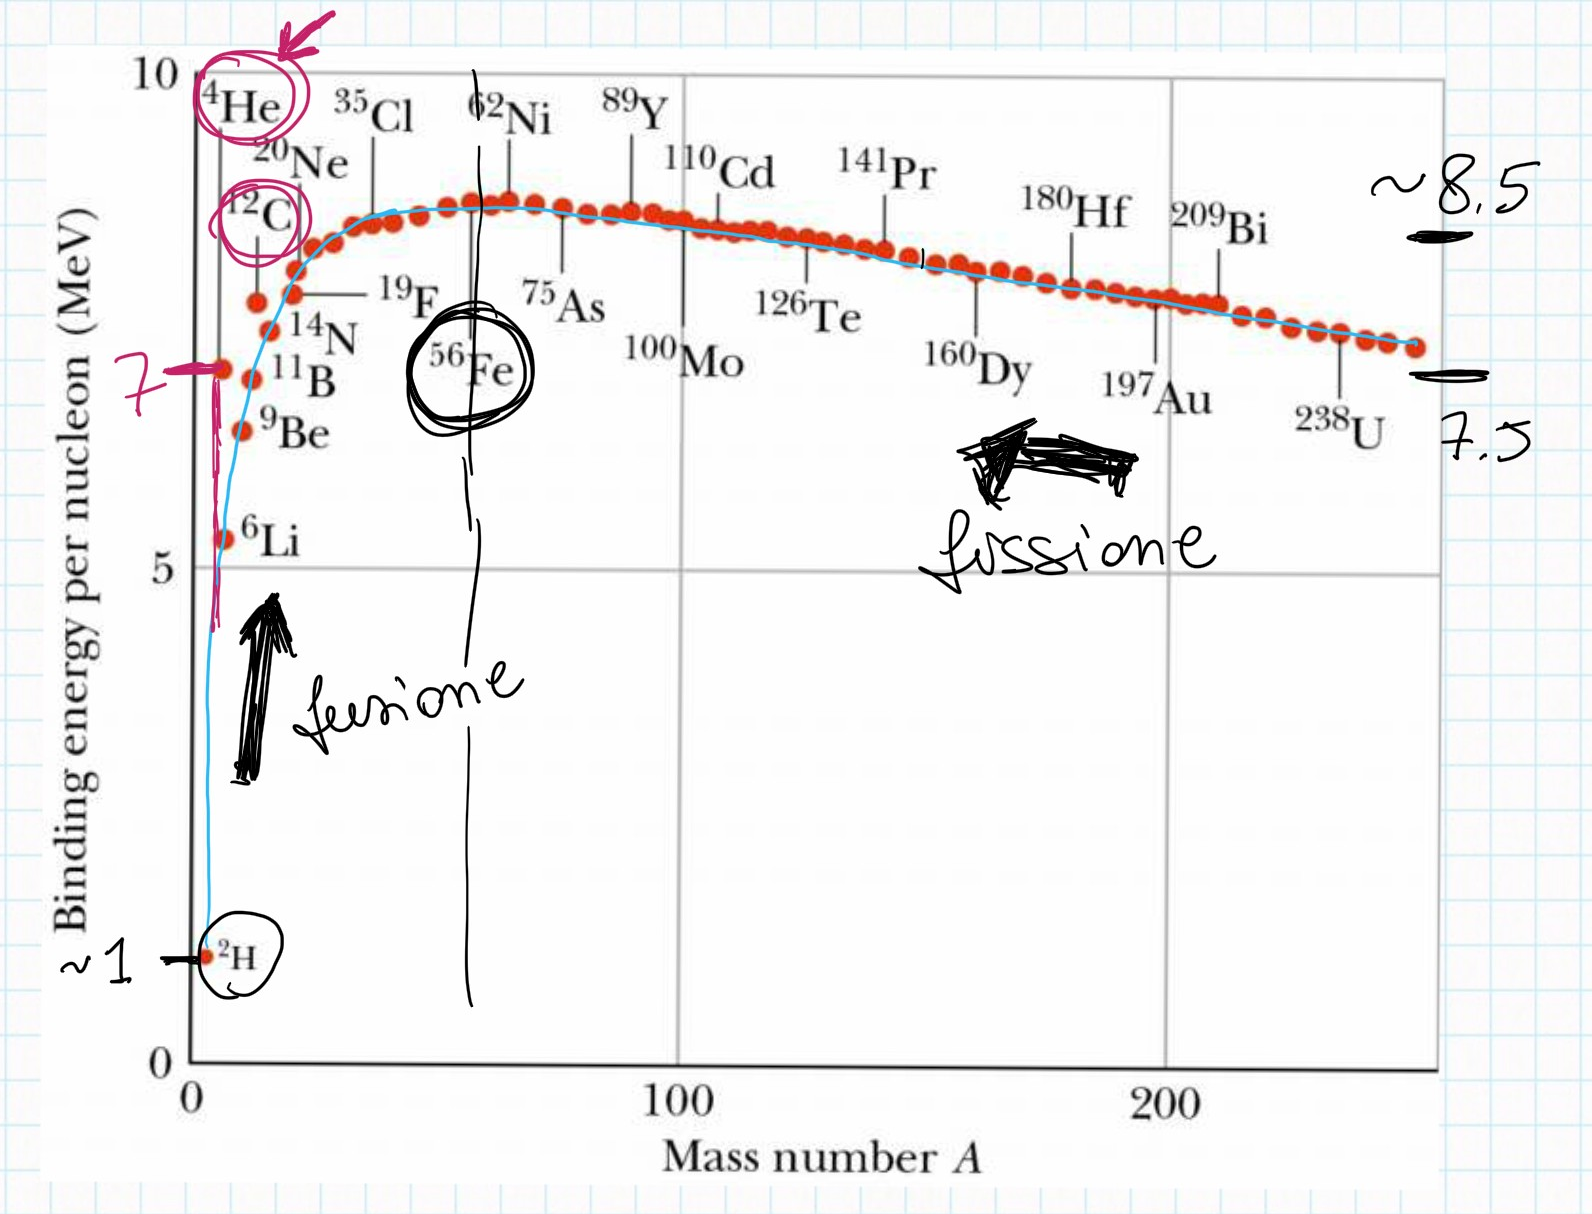
\includegraphics[scale=0.26]{Immagini/curva_elementi.png}
    \caption{Curva che rappresenta l'andamento dell'energia di legame al crescere del peso atomico. Sono segnati il picco del ferro, le reazioni in funzione dei pesi atomici e i salti dei nuclei di elio e carbonio.}
    \label{B/A}
\end{figure}

\subsection{Primi passi} 
Intanto osserviamo che il primo stato legato possibile è $A=2$ ovvero $\ce{^2_1H_1}$ e ha una $B\simeq 2.225$ MeV. Poi notiamo un picco nei d'intorni del $\ce{^56Fe}$:
\begin{itemize}
    \item Per $A<56$ allora si ha che \vir{salendo} anche l'energia di legame aumenta, dunque è favorita la \textbf{fusione nucleare}\footnote{Fa eccezione l'elio per cui si ha una $B\sim 28$ MeV; cercheremo di spiegare più avanti il motivo. Lo stesso vale per il carbonio.}:
    $$\ce{^{A_1}X} + \ce{^{A_2}Y} \to \ce{^AX}'$$
    \item Per $A>56$ \vir{salire} non è conveniente e vengono quindi privilegiati i processi di \textbf{fissione nucleare}:
    $$\ce{^AX}' \to \ce{^{A_1}X} + \ce{^{A_2}Y}$$
\end{itemize}
\noindent Osserviamo anche che eccetto i primi salti la curva si assesta intorno a valori compresi tra i $7.5 \% 8.5$ MeV e quindi prenderemo come valor medio per la maggior parte degli elementi 8 MeV.

\section{Formula Semi-empirica di massa}
Per $A$ \vir{sufficientemente grande} esiste una formula empirica che fitta abbastanza bene i dati.
\begin{definition}[\textbf{Formula Semi-empirica di Massa}]\index{formula semi-empirica di massa}
Esprime l'energia di legame per nuclei pesanti:
$$B = \underbrace{a_V \, A - a_S\, A^{2/3} - a_C \, \frac{Z(Z-1)}{A^{1/3}}}_\text{Modello a goccia} %
- \underbrace{a_{sym} \, \frac{(A-2Z)^2}{A}}_\text{Modello a shell nucleare} %
+\, \delta$$
\begin{displaymath}
\begin{aligned}
&\text{\textbf{Termine di Volume}} & &a_V = 15.5\;\mbox{MeV} & &\text{\textbf{Termine di Coulomb}} & &a_C = 0.72\;\mbox{MeV}\\
&\text{\textbf{Termine di Superficie}} & &a_S = 16.8\;\mbox{MeV} & &\text{\textbf{Termine Simmetrico}} & &a_{sym} = 23\;\mbox{MeV}\\
\end{aligned}
\end{displaymath}
\begin{displaymath}
\begin{aligned}
&\text{\textbf{Termine di Pairing}} & &\delta = \Biggl \{ 
\begin{array}{ll}
    34\;\mbox{MeV}\;\, A^{-3/4} &  \text{even-even}\\
    0 &  A\; \text{dispari}\\
    -34\;\mbox{MeV}\;\, A^{-3/4} & \text{odd-odd}
\end{array}
\end{aligned}
\end{displaymath}
\end{definition}
Passiamo adesso a illustrare il significato dei singoli coefficienti:
\begin{itemize}
    \item $a_V$:\index{formula semi-empirica di massa!termine di volume} il primo termine è lineare in $A$, per questo l'interazione nucleare è a corto raggio, ovvero è un'interazione di primi vicini. Si chiama termine di volume perché il raggio nucleare scala come $r\simeq r_0 A^{1/3}$, quindi il volume scala con $A$.
    \item $a_S$:\index{formula semi-empirica di massa!termine di superficie} i nucleoni sulla \vir{superficie} hanno ovviamente meno vicini di quelli più \vir{interni}, dunque dobbiamo tenere conto di questa assenza con un termine proporzionale alla superficie, cioè dall'andamento visto prima proporzionale a $A^{2/3}$.
    \item $a_C$:\index{formula semi-empirica di massa!termine di Coulomb} poiché la formula vale per atomi pesanti, spesso $Z\gg 1$ e il termine coulombiano viene riscritto come:
    $$a_C \frac{Z^2}{A^{1/3}}$$
    Questo deriva dall'espressione dell'energia coulombiana $\sim Q^2/R = Z^2 e^2 / (r_0A^{1/3})$; allora $a_C \propto e^2/r_0$.
    \item $a_{sym}$:\index{formula semi-empirica di massa!termine simmetrico} questo è un termine puramente quantistico e può essere riscritto come\footnote{Si usa solo $A=Z+N$.}:
    $$(A-2Z)^2 = (N-Z)^2$$
    Si vede allora che per $N=Z$ questo termine scopare, ovvero il nucleo è più stabile; questo è confermato dalle osservazioni solo per $A$ \vir{non troppo grandi}, come si vede in Figura \ref{segre}, quindi si divide per $A$.
    \item $\delta$: esistono solo 6 nuclei stabili in natura con $A$ pari e $N$ e $Z$ dispari.
\end{itemize}
\noindent Infine valgono le seguenti disuguaglianze:
$$a_C \lll a_V <a_S < a_{sym}$$

\begin{figure}[h]
    \centering
    \textbf{\Large Carta di Segré}\index{carta di Segré}\par\medskip
    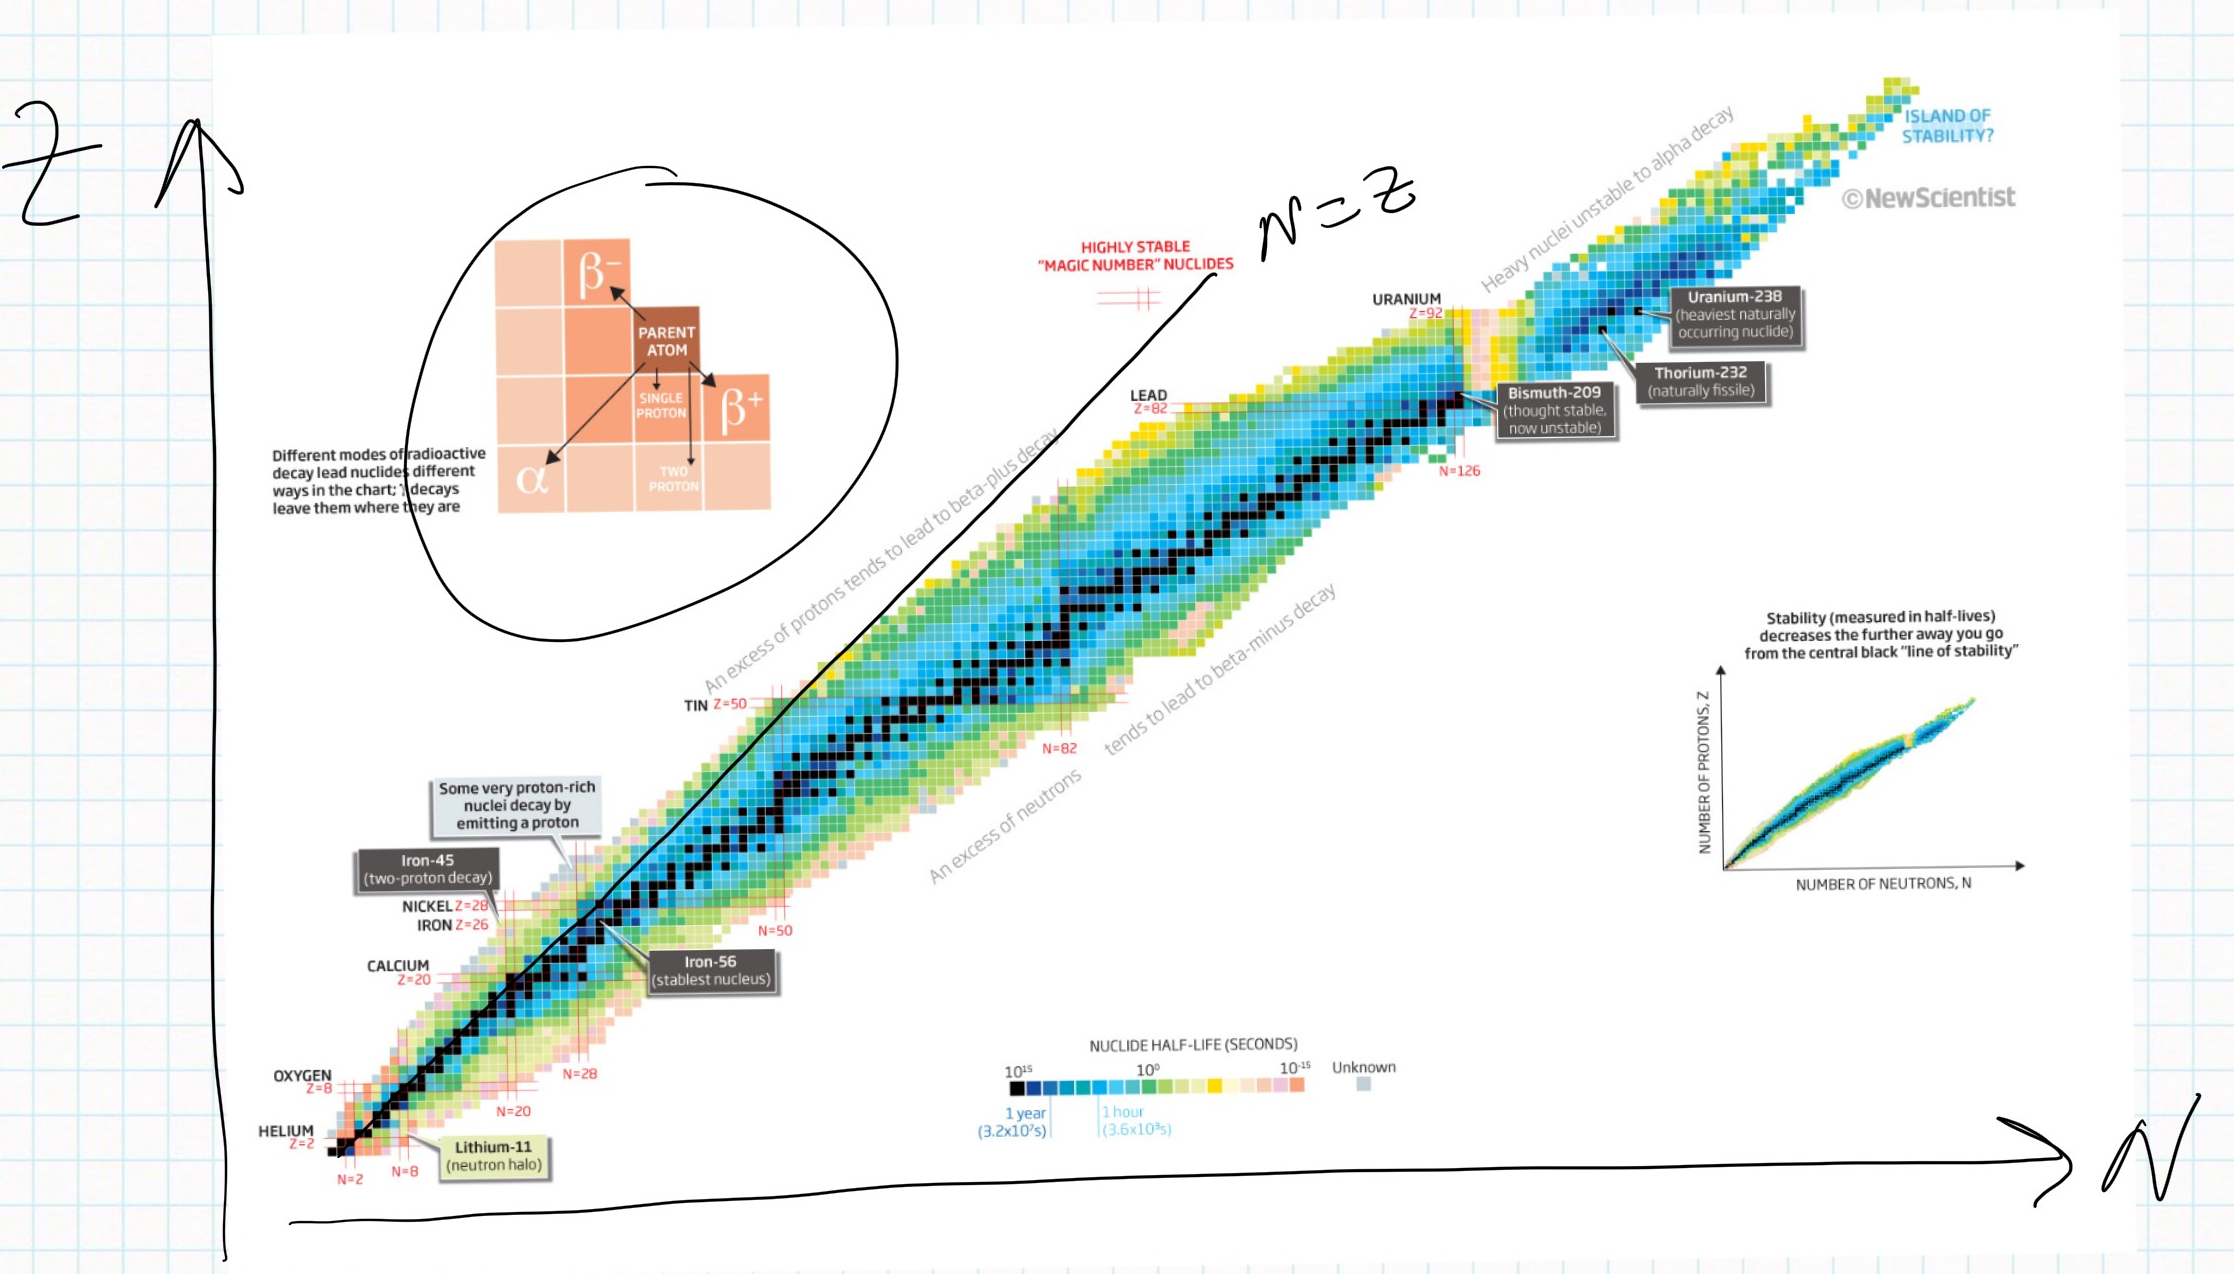
\includegraphics[scale=0.21]{Immagini/Segre.png}
    \caption{Sono riportati i nuclei in base a $Z$ e $N$. La linea centrale viene chiamata \textbf{valle di stabilità}\index{valle di stabilità}. Indicativamente dopo il Ca non vale più $N=Z$ per i nuclei stabili. In alto sono riportati i decadimenti.}
    \label{segre}
\end{figure}
\newpage
\section{Decadimenti}
Illustriamo i principali decadimenti.

\paragraph{Decadimento $\alpha$} Mediato dall'interazione forte perché sia nello stato iniziale che nel finale ho solo nuclei:
$$\alpha: \qquad \ce{^A_ZX_N} \to \ce{^{A-4}_{Z-2}Y_{N-2}} + \alpha $$
\paragraph{Decadimenti $\beta$} Mediati dall'interazione debole:
$$\beta^-: \qquad \ce{^A_ZX_N} \to \ce{^{A}_{Z+1}Y_{N-1}} + e^- + \bar{\nu}_e \quad \text{Dentro il nucleo}\quad n \to p + e^- + \bar{\nu}_e $$
$$\beta^+: \qquad \ce{^A_ZX_N} \to \ce{^{A}_{Z-1}Y_{N+1}} + e^+ + \nu_e \quad \text{Dentro il nucleo}\quad p \to n + e^+ + \nu_e$$
\noindent Procediamo adesso con una \vir{dimostrazione} della stabilità dei nuclei con $N=Z=A/2$ per $Z\lsim 20$.\\
Per primo scriviamo la massa di un generico nucleo in funzione di $Z$ e $A$:
$$m(\nuc{X}{A}{Z}{N}) = Zm_p + Nm_n - B(Z,A) \simeq Z m(\ce{^1H}) + (A-Z)m_n- B(Z,A)$$
Fissato $A$ cerchiamo il minimo di $m$ al variare di $Z$.
$$\frac{\partial m}{\partial Z} = 0 \;\Rightarrow\; m(\ce{^1H})-m_n + 2a_C \frac{Z}{A^{1/3}} - \frac{a_C}{A^{1/3}}-4a_{sym}\frac{A-2Z}{A} = 0$$
$$Z_{\min} = \frac{m_n - m(\ce{^1H})+a_C A^{1/3}+4 a_{sym}}{2[a_CA^{1/3}+4a_{sym}A^{-1}]}\simeq \frac{A}{2}$$
dove nell'ultima approssimazione abbiamo usato che $m(\ce{1H})\simeq m_n$ e che $a_C\ll a_{sym}$, per cui per $A$ piccolo (ma non troppo) si può trascurare il termine $a_C A^{1/3}$ nel denominatore.\\
Dato che l'andamento di $B\propto Z^2$ allora possiamo rappresentare\footnote{Qui trattiamo $Z$ come una variabile continua per ottenere gli andamenti.} approssimativamente l'andamento di $M$ al variare di $Z$, come in Figura \ref{MvsZ}.\\
È molto raro ma è possibile osservare anche un decadimento doppio $\beta$ indicato $2\nu\beta\beta$; quello che si cerca di osservare è un doppio $\beta$ senza neutrino, ovvero $\phi \nu \beta\beta$, poiché in questo caso si avrebbe una violazione dello \textit{standard model}, il neutrino non sarebbe una particella di Dirac, ma di Mayorana per cui $\nu = \bar{\nu}$.

\begin{figure}[!h]
    \centering
    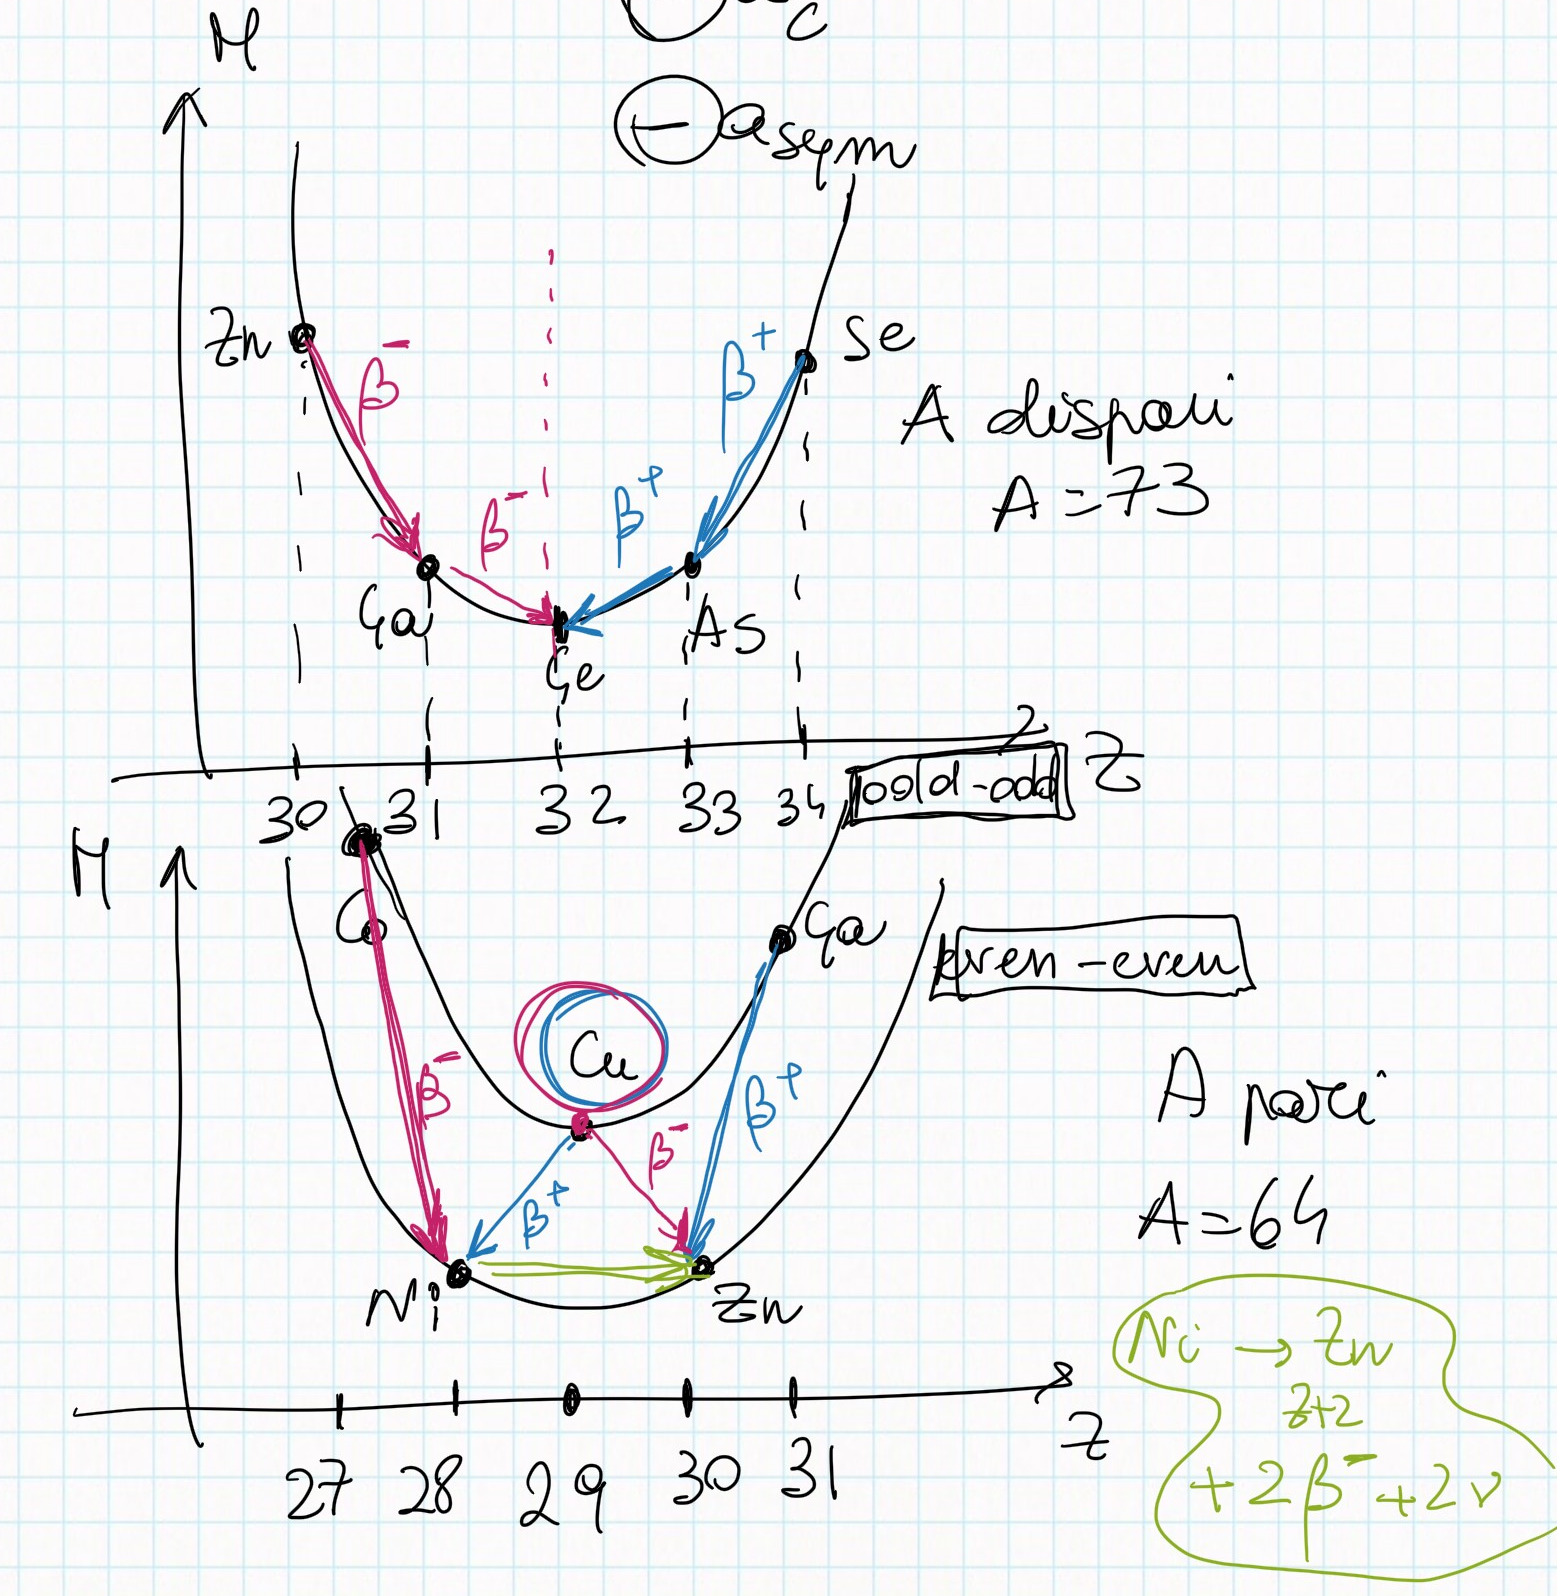
\includegraphics[scale=0.3]{Immagini/MvsZ.png}
    \caption{Rappresentazione di $M$ in funzione di $Z$. Si osserva che per i nuclei con $A$ dispari si hanno decadimenti $\beta^-$ scendendo verso destra, mentre $\beta^+$ scendendo verso sinistra. Per i nuclei con $A$ pari il termine di pairing nell'energia di legame si fa sentire e questo porta a nuclei che possono avere sia $\beta^+$ che $\beta^-$ (in questa configurazione i doppio $\beta$ sono praticamente inesistenti).}
    \label{MvsZ}
\end{figure}

\begin{curiosita}
In Fisica Medica viene utilizzato il $\ce{^64Cu}$ poiché può sia decadere $\beta^+$ che $\beta^-$; il decadimento $\beta^+$ viene usato per la PET, mentre il $\beta^-$ per l'uccisione dei tumori
\end{curiosita}

\section{$Q$-value}
Dato un processo\footnote{Come sempre $c=1$} $A+B\to C+D$ si definisce $Q$-value:
$$Q = m_A + m_B - m_C - m_D$$
Si hanno allora:
\begin{itemize}
    \item[-] $Q>0$ \textbf{esotermico} (spontaneo); l'energia relativa può essere nulla. 
    \item[-] $Q<0$ \textbf{endotermico} (non spontaneo); l'energia relativa dev'essere positiva.
\end{itemize}
\newpage

    %   15/02
%%  Modello a shell
%\part*{Lezione 01/03/2021}
\chapter{Modelli nucleari}
In questo capitolo introduciamo e discutiamo i modelli nucleari \textit{a shell} e \textit{a goccia}. Il capitolo copre le Lezioni del 01/03/2021 e del 03/03/2021.

\paragraph{Introduzione} Se il sistema a due nucleoni è \vir{complicato}, quando $A$ diviene proibitivo è necessario ricorrere a modelli per descrivere le proprietà nucleari\footnote{Per un testo di riferimento sull'argomento vedi \complrif{compl-krane}.}. Dall'analogia con la fisica atomica, il modello \vir{più semplice} che approfondiremo per primo è appunto un modello di tipo \textit{a shell}.

\section{Primi passi per il modello \textit{a shell}}
Nel caso della fisica atomica un modello \textit{a shell} è supportato dagli andamenti del raggio atomico e dell'energia di ionizzazione (Figura \ref{0301_rE}), i cui salti possono essere associati  appunto alla \vir{chiusura} di uno \textit{shell}. In questo modello gli elettroni si muovono in un campo esterno generato dal nucleo, senza collidere tra loro.\\
Applicare tutto ciò alla fisica nucleare non è immediato: i nucleoni, infatti, \vir{vivono} in un potenziale che non è esterno, ma generato da essi stessi e le loro dimensioni non sono trascurabili rispetto alle dimensioni del nucleo.
\begin{figure}[!h]
    \centering
    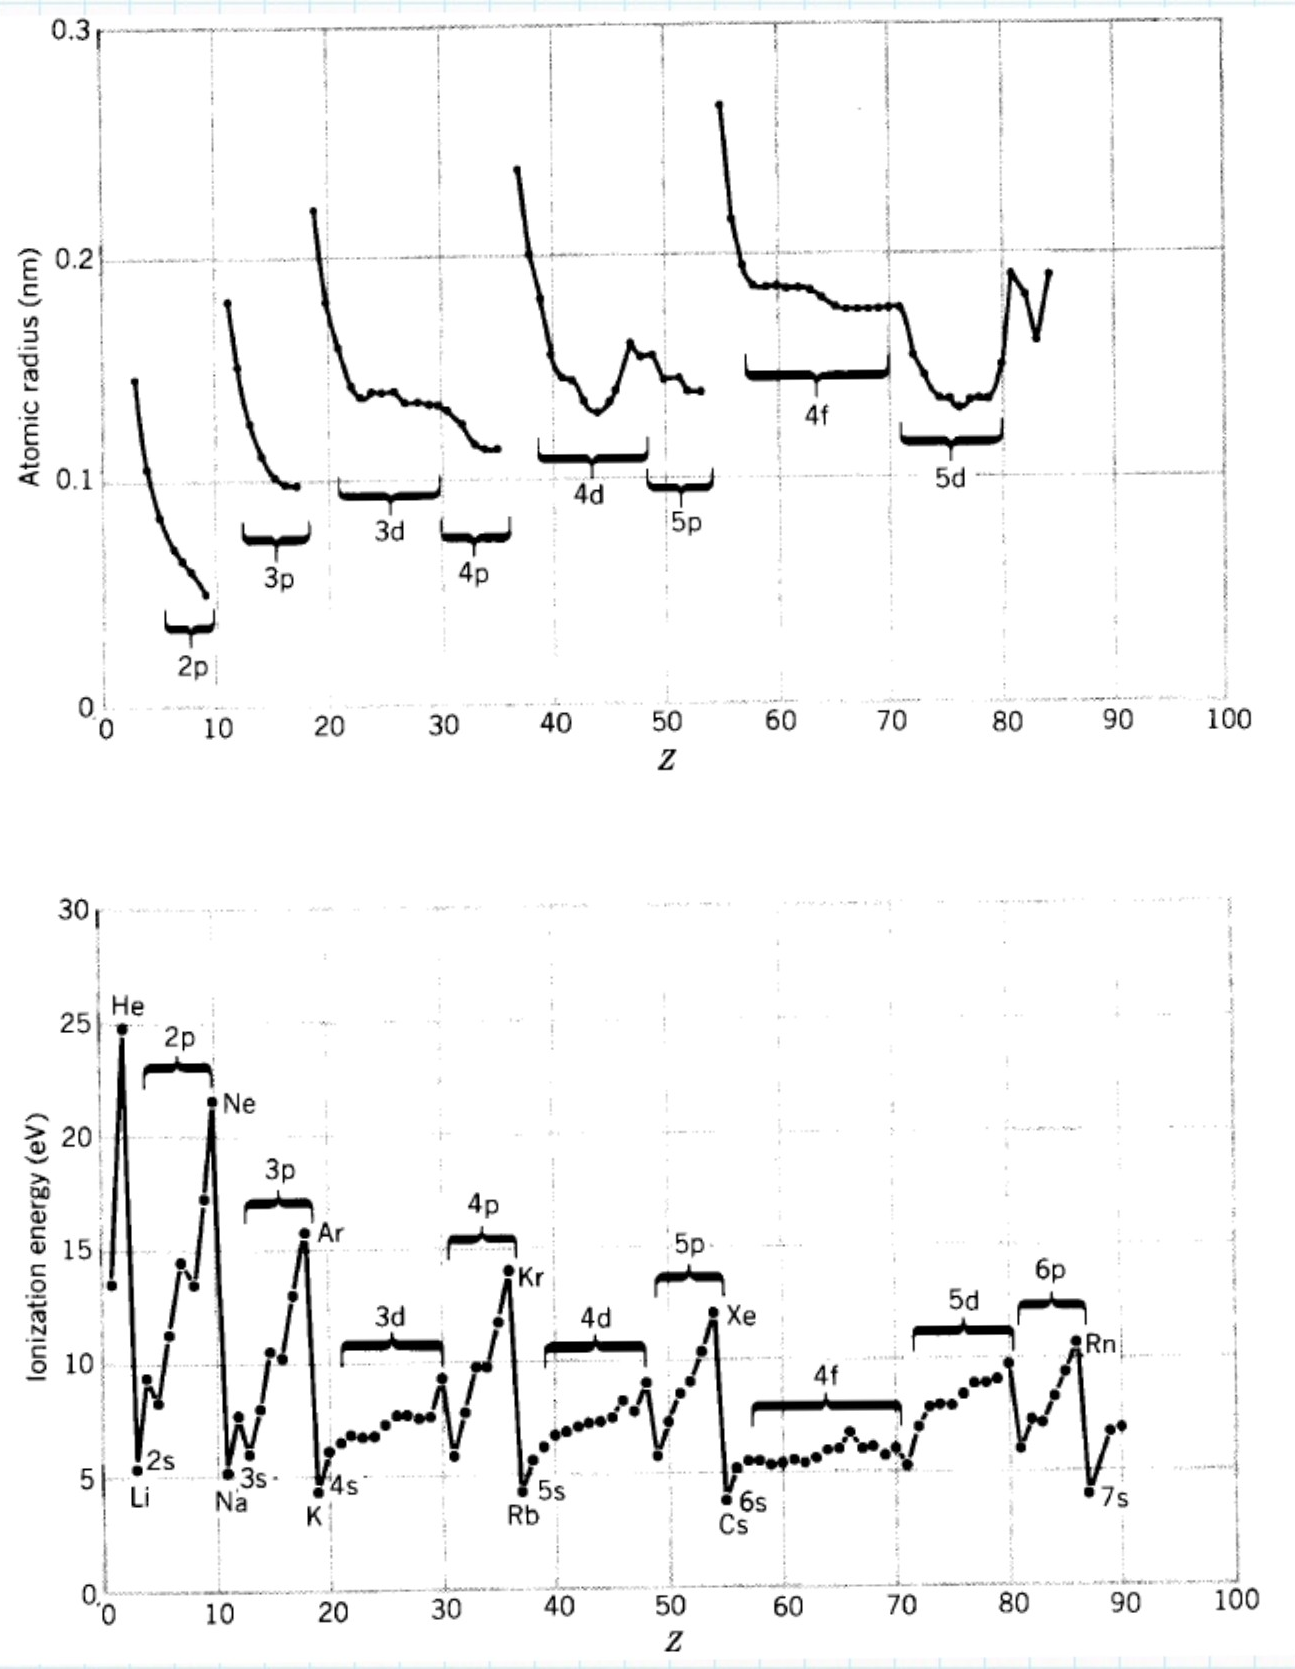
\includegraphics[scale=0.2]{Immagini/ratm-Eion.png}
    \caption{Andamento in alto del raggio atomico e in basso dell'energia di ionizzazione al variare del numero atomico. I salti sono ben spiegati da un modello \textit{a shell}.}
    \label{0301_rE}
\end{figure}
\newline
Tuttavia, vi sono alcune evidenze sperimentali a favore di tale modello. Innanzitutto, le differenze di energia di separazione\footnote{Sono le energie di separazione del protone e del neutrone rispettivamente.} tra nuclei con $N=\mbox{cost}$ (\textbf{isotoni}\index{nucleo!isotono}) e nuclei con $Z=\mbox{cost}$ (\textbf{isotopi}\index{nucleo!isotopo}) hanno salti ben determinati\footnote{Dovrebbe comparire anche il 2, ma non lo vedo perché corrisponde alla separazione di 2 protoni. Per quanto riguarda il 126 non si vede in natura nel caso di $Z$, perché il nucleo non è stabile.}, come mostrato in Figura \ref{diffeng}. I numeri atomico o neutronico per i quali si hanno i salti richiamano i numeri quantici di un modello \vir{a shell} e vengono definiti \textbf{numeri magici}\index{numeri magici}:
$$2,8,20,28,50,82,126$$
\begin{figure}[!h]
    \centering
    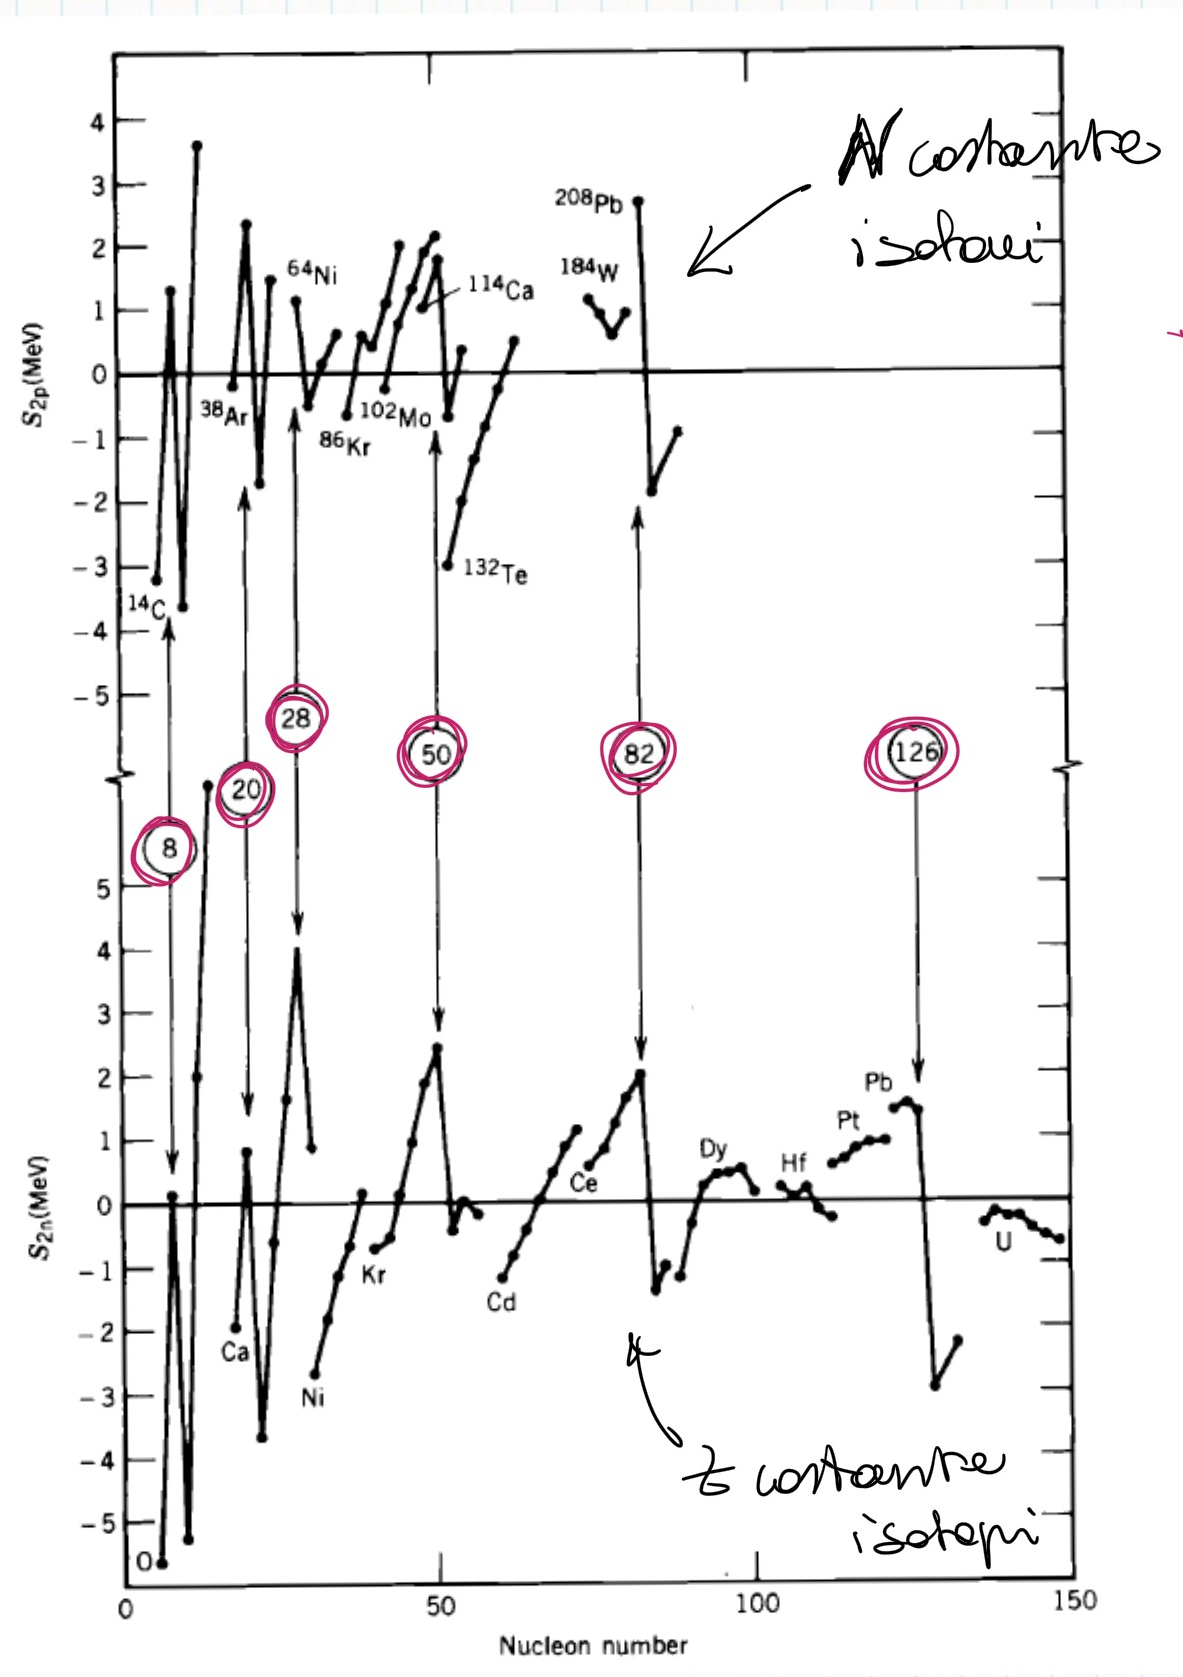
\includegraphics[scale=0.2]{Immagini/mag-num.png}
    \caption{In alto l'andamento dell'energia di separazione degli isotoni $S_n$ e in basso quello dell'energia di separazione degli isotopi $S_p$. Al centro sono riportati i numeri magici.}
    \label{diffeng}
\end{figure}

\noindent Un'altra evidenza consiste negli andamenti della sezione d'urto di cattura neutronica $\sigma$ e dei raggi di carica nucleari, riportati in Figura \ref{sigmar}, che ricordano quello del raggio atomico.

\begin{figure}[!h]
    \centering
    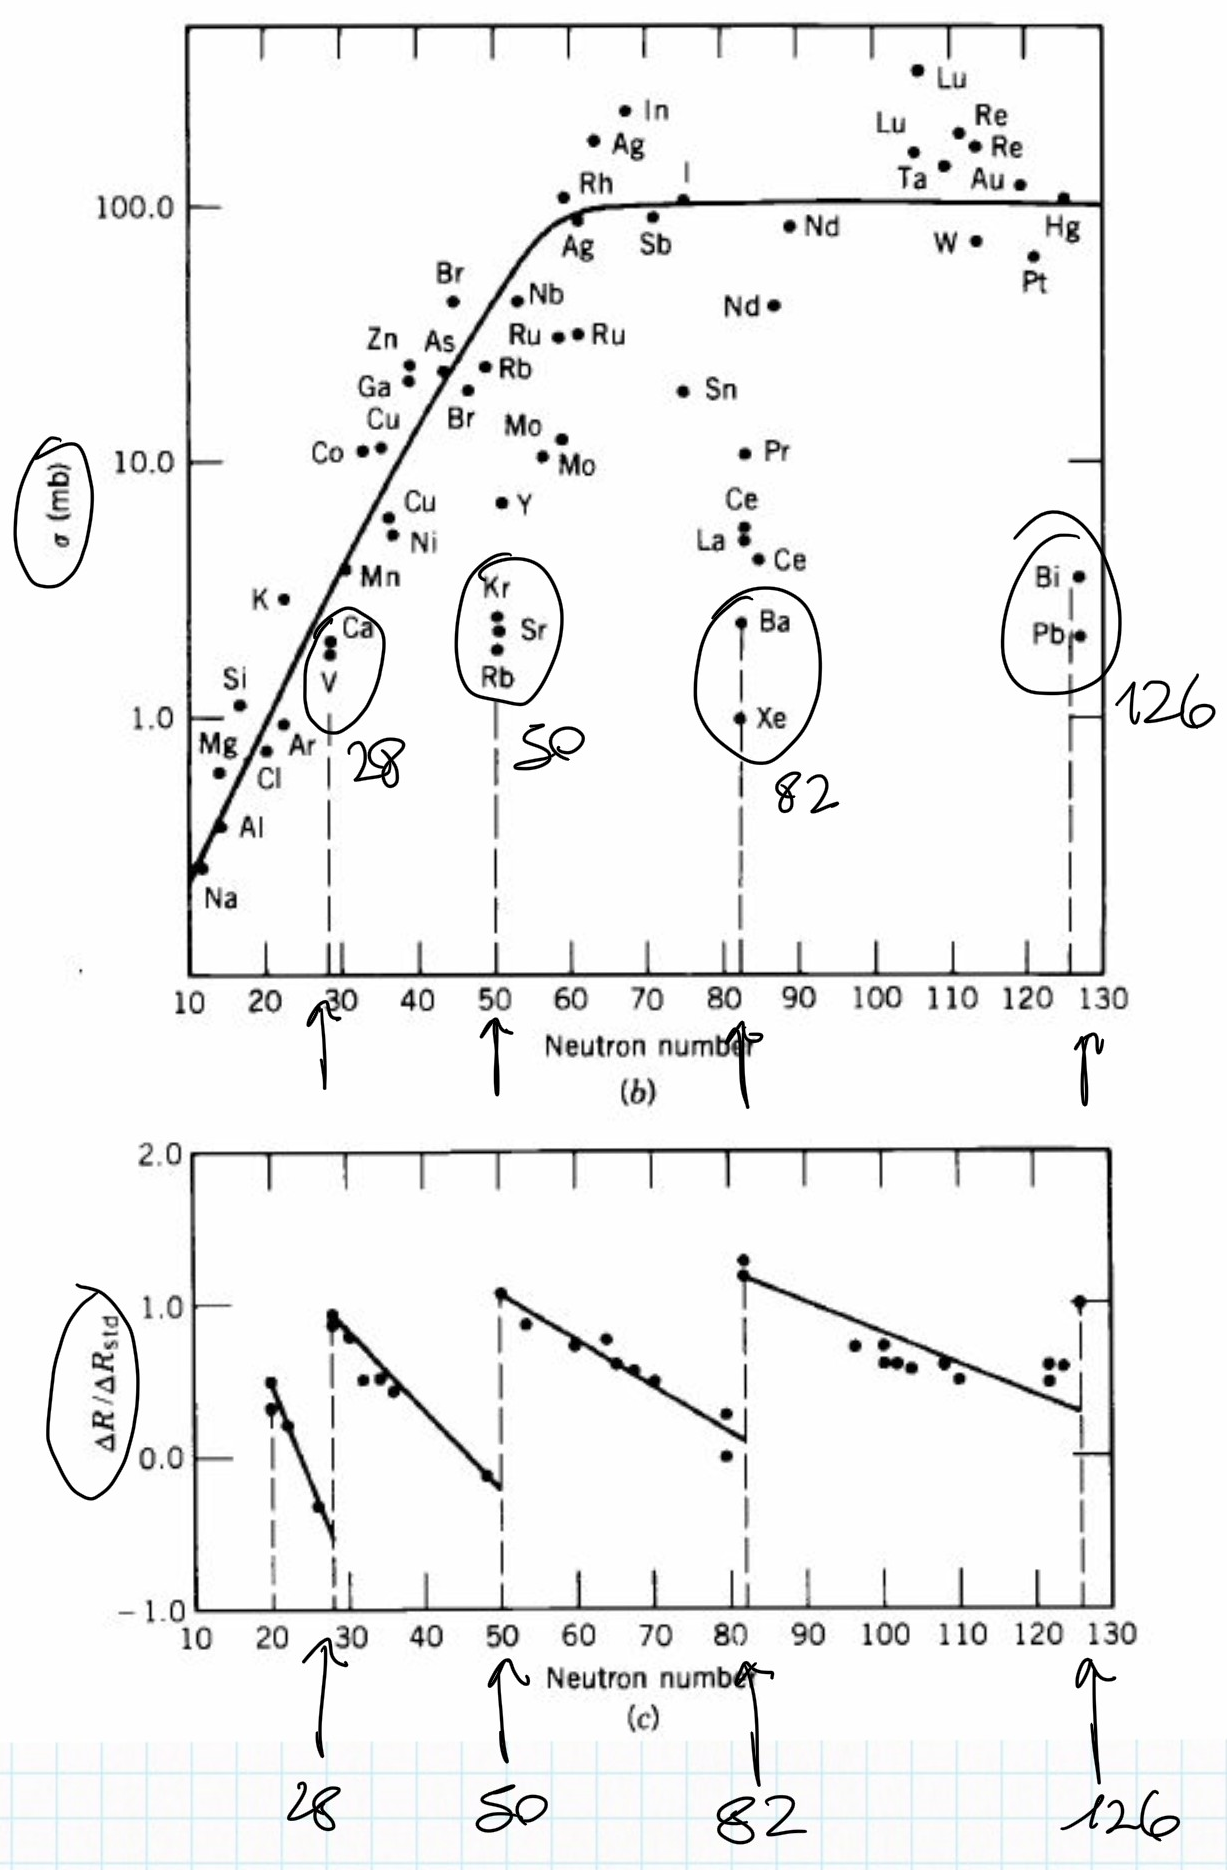
\includegraphics[scale=0.3]{Immagini/mag-num2.png}
    \caption{Andamenti della sezione d'urto $\sigma$ in alto e dei raggi di carica in basso in funzione del numero di neutroni nel nucleo. Si osservano salti in corrispondenza dei numeri magici.}
    \label{sigmar}
\end{figure}
\newpage
\section{Modello \textit{a shell}}
\index{modelli nucleari! a shell@\textit{a shell}}
\subsection{Sciogliamo i nodi} 
Innanzitutto risolviamo i problemi che ci eravamo posti nella formulazione del modello.
Assumiamo che il moto del singolo nucleone sia governato dal potenziale generato da tutti gli altri con i quali interagisce, escluso esso stesso. Per quanto riguarda gli urti, essendo i nucleoni fermioni se avvenisse una collisione (quindi un trasferimento di energia) questo comporterebbe una promozione a un livello di valenza (unico disponibile per Pauli), ma le energie richieste per far ciò sono notevolmente maggiori di quelle scambiabili attraverso l'urto. Dunque, assumeremo che gli urti non avvengono.\\[-1cm]
\paragraph{Calcolo della funzione d'onda} Dobbiamo ovviamente soddisfare all'equazione di \Sch, tuttavia per semplificare il calcolo possiamo prima rimaneggiare l'hamiltoniana del sistema: 
$$H=\sum_i T_i + \sum_{i<j}V_{ij}$$ 
con $T_i$ l'energia cinetica e $V_{ij}$ il potenziale di interazione. Sommando e sottraendo il potenziale $U_i$ che sente la $i$-esima particella a causa degli altri $j\not =i$ nucleoni, si ottiene:
\begin{displaymath}
\begin{aligned}
H&=\sum_i T_i + \sum_{i<j}V_{ij} +\sum_i U_i - \sum_i U_i=\\
&= \sum_i (T_i + U_i) + \Bigl [ \sum_{i<j} V_{ij} - \sum_i U_i \Bigr ] \simeq\\
&\simeq \sum_i (T_i + U_i)\\
H_i &\simeq T_i + U_i
\end{aligned}
\end{displaymath}
dove nell'ultimo passaggio abbiamo trascurato il contributo dato dal potenziale residuo, perché se $U_i$ è una buona approssimazione del campo che risente $i$ allora quella differenza è molto \vir{piccola}. Otteniamo così un'hamiltoniana di singola particella, per cui $H_i \psi_i = \varepsilon_i \psi_i$, con $\psi = \Pi_i \psi_i$ e $E = \sum_i \varepsilon_i$. Data la natura dei fermioni, cerchiamo una $\psi$ antisimmetrica, che otteniamo tramite il determinante di Slater\footnote{Per puro scopo esemplificativo riportiamo il caso $N=2$:
$$\psi (\xi_1,\xi_2) = \psi_1 (\xi_1)\psi_2 (\xi_2) - \psi_2 (\xi_1)\psi_1 (\xi_2)$$}:
\begin{displaymath}
\psi = \det
\begin{vmatrix}
\psi_1 (\xi_1) & \psi_1 (\xi_2) & \dots & \psi_1 (\xi_N) \\
\psi_2 (\xi_1) & \psi_2 (\xi_2) & \dots & \psi_2 (\xi_N) \\
\vdots         &                & \ddots&                \\
\psi_N (\xi_1) & \psi_N (\xi_2) & \dots & \psi_N (\xi_N)
\end{vmatrix}
\end{displaymath}
Rimane quindi da scegliere il potenziale $U_i$.
\begin{itemize}
    \item \textbf{Potenziale a buca infinita}: conosciamo già la soluzione per gli stati legati\footnote{Mettiamo $\hbar=1$.}, ovvero $\psi = A \sin (kx) + B \cos (kx)$, con $k\equiv \sqrt{2mE}$. Dalle condizioni ai bordi $\psi(0)=\psi(a)=0$, si ha $ka = n\pi$ per cui $\varepsilon_n = \hbar^2 \pi^2  n^2 / 2ma^2$.
    \item \textbf{Potenziale armonico} $V(x)=Kx^2/2$: anche in questo caso sappiamo che le soluzioni sono della forma $\psi(x) = H(x)\exp{(-\alpha x^2/2)}$, con $\alpha \equiv \sqrt{Km}$ e $H(x)$ polinomio di Hermite, il cui grado dà l'energia. Si ha quindi nel caso unidimensionale $\varepsilon_n = \hbar \omega_0 (n+1/2)$, dove $\omega_0 \equiv \sqrt{K/m}$, da cui generalizzando $E_N= \hbar \omega_0 (N+3/2)$, con $N= n_x+n_y+n_z$.
    \item \textbf{Buca Wood-Saxon}\index{buca di Wood-Saxon}: in questo caso il conto è un po' più complicato, lo vedremo successivamente; intanto riportiamo soltanto l'espressione di questo potenziale:
    $$V(x) = - \frac{V_0}{1+\exp{(\frac{r-R}{a})}}$$
    dove $V_0$ è la profondità della buca in $r=0$, $R$ è il raggio medio e $a$ è quella che viene chiamata \textit{skin thickness}\footnote{Questi dettagli sono stati presi da Krane, K., S., \textit{\vir{Introductory Nuclear Physics}}, USA, John Wiley \& Sons, 1988.}.
\end{itemize}
\noindent Come per il modello \textit{a shell} atomico usiamo la notazione spettroscopica per cui $N = 2(n-1)+\ell$, dove $n$ non è però il numero quantico principale (tiene conto solo del numero di livelli con un certo $\ell$) e $\ell$ è il momento angolare. Considerando anche lo \textit{spin}, abbiamo una \textbf{degenerazione dello stato energetico} pari a: $2(2\ell+1)$, per cui:
\begin{displaymath}
\begin{aligned}
&N & n&,\ell & \text{orb}&\text{itale} & \text{Numero}&\text{ nucleoni} & \text{To}&\text{tale}\\
&0 & 1&,0 & &1s & &2 & &2   \\
&1 & 1&,1 & &1p & &6 & &8   \\
&2 & 1,2&;2,0 & 1d&;2s & 10&+2 & &20 \\
&3 & 1,3&;2,1 & 1f&;2p & 14&+6 & &40   \\
&4 & 1,4;2&,2;3,0 & 1g;2&d;3s & 18+&10+2 & &70
\end{aligned}
\end{displaymath}
Osserviamo che il numero totale di nucleoni nei primi 3 livelli pieni corrisponde proprio ai primi 3 numeri magici, ma dal quarto in poi la sequenza non è più rispettata; con questo tipo di potenziale infatti riesco a spiegare bene solo le prime 3 configurazioni, come mostrato in Figura \ref{shell} e in Figura \ref{shellmix} a sinistra.
\begin{figure}[h]
    \centering
    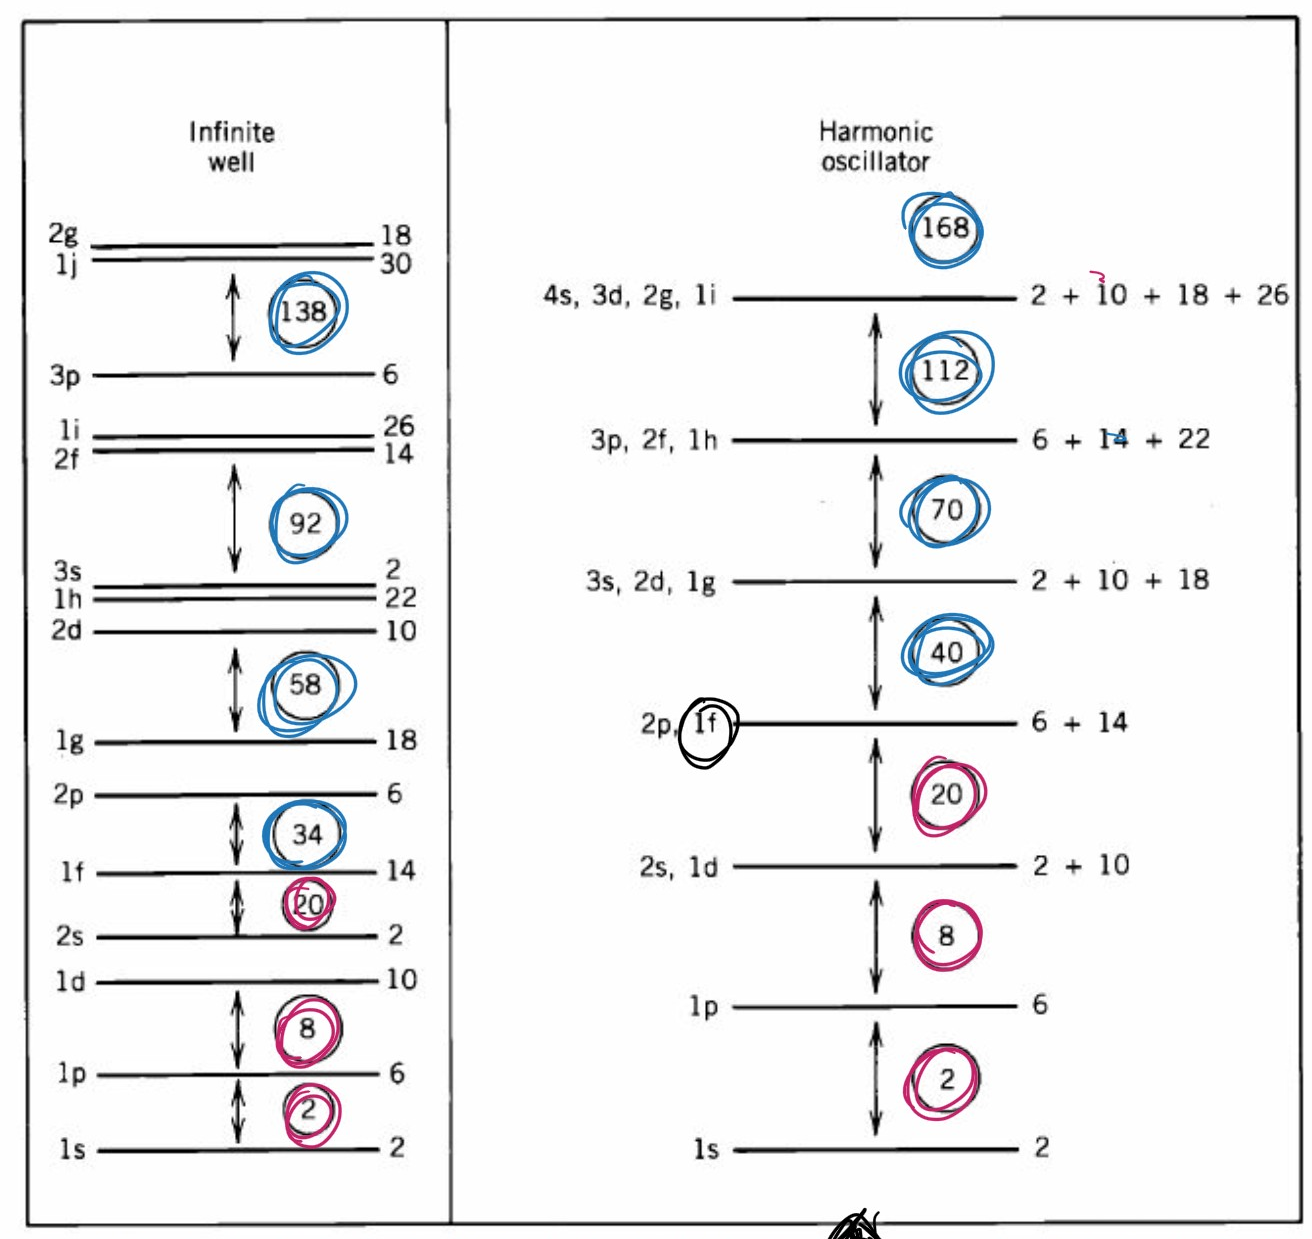
\includegraphics[scale=0.25]{Immagini/shell.png}
    \caption{Sequenza degli orbitali a sinistra con potenziale a buca e a destra con potenziale armonico.}
    \label{shell}
\end{figure}

\subsection{Modello \textit{a shell} + spin-orbita}
Consideriamo adesso il potenziale di Wood-Saxon (più realistico della buca e dell'armonico) e teniamo conto dell'interazione \textit{spin}-orbita\footnote{Di questa ne abbiamo evidenze nello scattering neutrone-neutrone}:
$$U (r) = V_{WS}(r) +  V_{s-o}(r)\; \vec{\ell} \cdot \vec{s} $$
$$ H \to T+V_{WS}(r)+V_{s-o}(r)\;\vec{\ell} \cdot \vec{s}$$
dove abbiamo omesso le $i$ ai pedici per semplicità. Aver introdotto questa interazione, però, rende $\ell_z$ e $s_z$ non più dei buoni numeri quantici poiché non commutano con $\vec{\ell}\cdot\vec{s}$; consideriamo allora il momento angolare totale $\vec{j}= \vec{\ell} + \vec{s}$ ed esprimiamo $\vec{\ell}\cdot\vec{s}$ in funzione di $j$ (per il singolo nucleone):
$$\mean{\vec{\ell}\cdot\vec{s}} = \frac{1}{2}\Bigl[j(j+1) - \ell(\ell+1) - \frac{3}{4} \Bigr]$$
Proviamo a questo punto a descrivere la configurazione $1f$ ($n=1,\ell=3$), che era la prima a non rispettare la sequenza dei numeri magici: abbiamo $j=5/2,7/2$ con degenerazione $2j+1$, per cui $1f_{5/2}$ ha 6 nucleoni e $1f_{7/2}$ ha 8 nucleoni\footnote{Questo ci piace perché sommato all'orbitale precedente si ottiene proprio 28.}. Per fare i conti, supponiamo che $V_{s-o}$ sia una buca rettangolare di profondità $V_0$, allora:
$$\diag{1f_{7/2}}{U_{s-o}} \sim - \frac{V_0}{2}\Bigl[ \frac{7}{2}\cdot\frac{9}{2} - 3\cdot 4 - \frac{3}{4} \Bigr] = -\frac{3}{2} V_0$$
$$\diag{1f_{5/2}}{U_{s-o}} \sim - \frac{V_0}{2}\Bigl[ \frac{5}{2}\cdot\frac{7}{2} - 3\cdot 4 - \frac{3}{4} \Bigr] = 2 V_0$$
Abbiamo che i due stati sono separati e la configurazione $1f_{7/2}$ si avvicina agli orbitali precedenti, per cui si ha un rimescolamento degli \textit{shell} che determina la sequenza dei numeri magici, come mostrato in Figura \ref{shellmix}.
\begin{figure}[h]
    \centering
    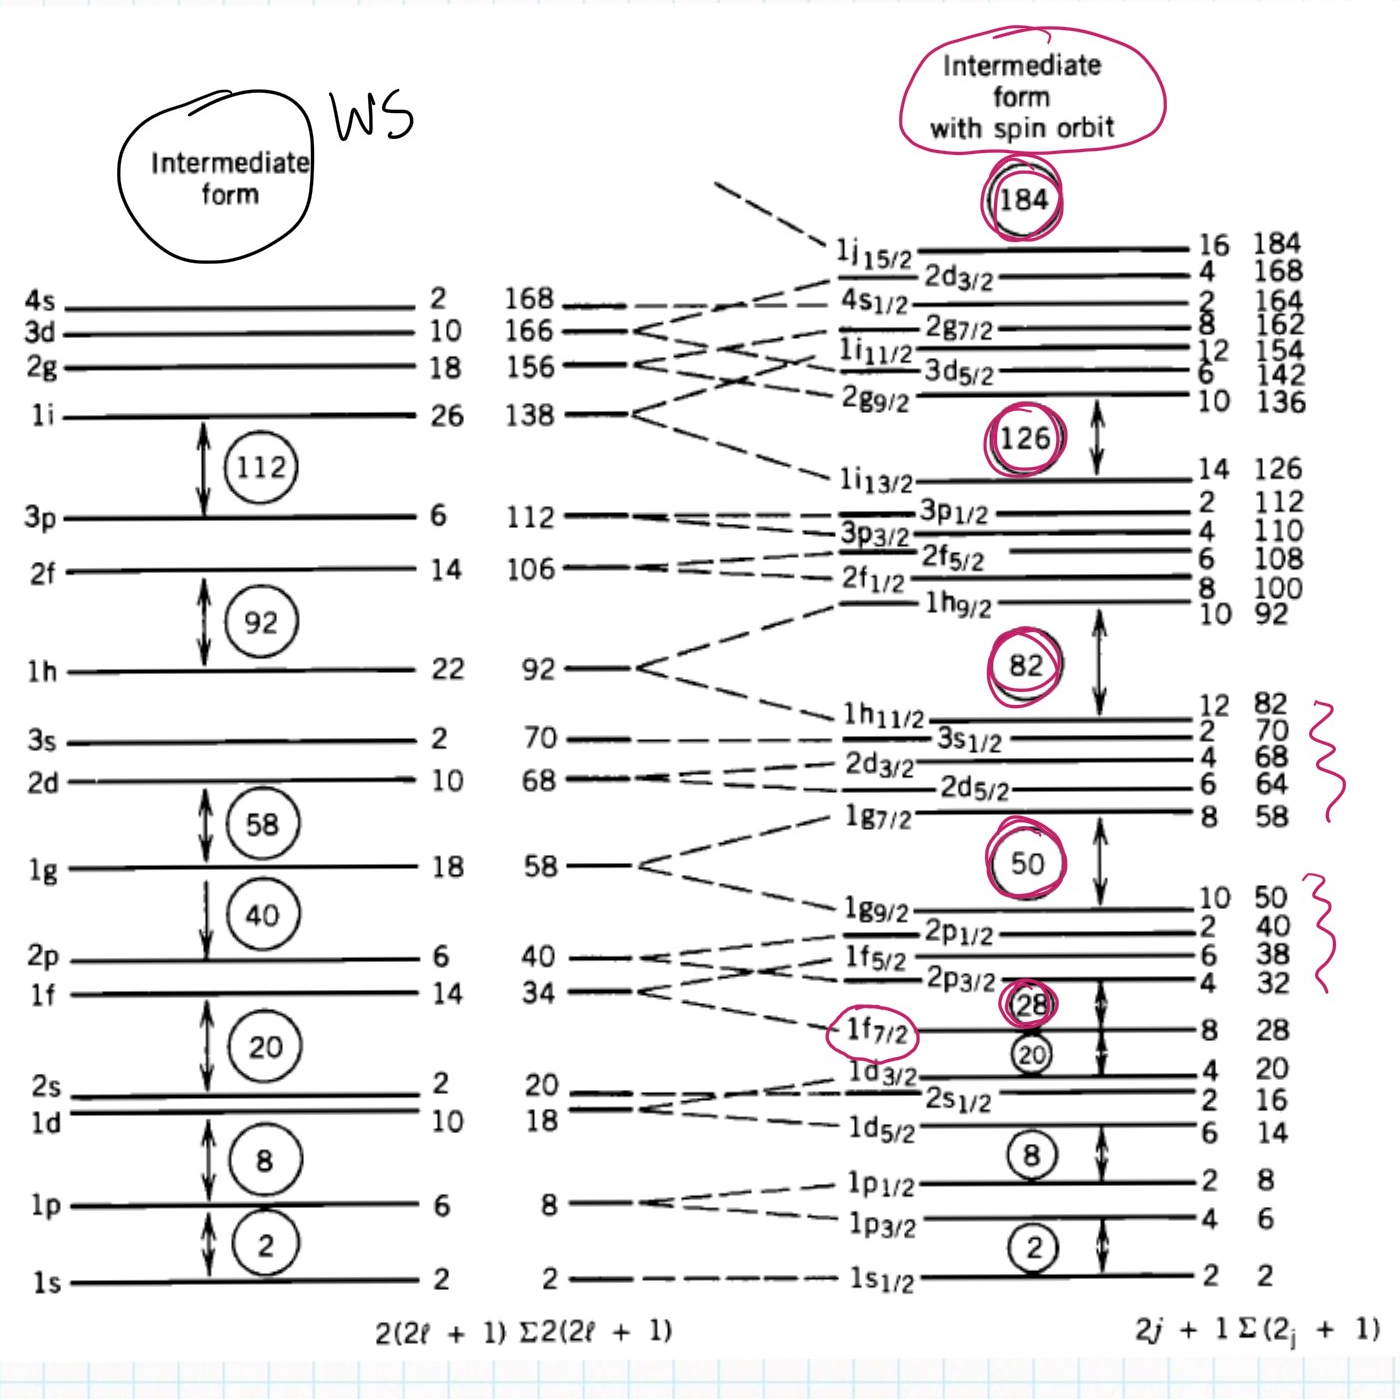
\includegraphics[scale=0.3]{Immagini/shell2.png}
    \caption{Configurazioni degli orbitali a sinistra con un potenziale di Wood-Saxon senza interazione \textit{spin}-orbita e a destra con lo stesso potenziale ma considerando tale interazione. Si vedono i rimescolamenti degli \textit{shell} e i numeri magici. Nella figura è presente un errore: è segnato $2f_{1/2}$ invece di $2f_{7/2}$.}
    \label{shellmix}
\end{figure}
%\noindent Dalla figura vediamo che c'è uno \textit{splitting} anche nella configurazione $1p$ e in altre, ma questi sono piccolissimi.

\subsubsection{I successi del modello} 
Questo modello è valso un premio Nobel, non solo perché riproduce i numeri magici, ma anche perché spiega varie evidenze sperimentali. Per esempio, giustifica il fatto che nuclei doppiamente magici, ovvero con sia $N$ che $Z$ numeri magici (come $\ce{^4_2He_2}$, $\ce{^{16}_8O_8}$,\dots), siano fortemente legati e la presenza del $J^\pi = 0^+$ per il fondamentale di tutti i nuclei pari-pari (tutti i nucleoni sono accoppiati). Il modello\footnote{In realtà questo è \textit{extreme indipendent particle model}.}, infatti, permette di descrivere le prorpietà dell'intero sistema dallo stato di un singolo nucleone spaiato.
Maggior successo fu appunto la previsione del $J^\pi$ dei nuclei pari-dispari con un solo nucleone disaccoppiato. Prendiamo a esempio $\ce{^{17}_8O_9}$: osserviamo che, secondo il modello, ha un neutrone spaiato nel livello $1d_{5/2}$ ed è di conseguenza questo che determina il $J^\pi$ del nucleo nel fondamentale, che è appunto $J^\pi=\frac{5}{2}^+$. Il $\ce{^15_8O_7}$ ha invece un neutrone spaiato nello stato $1p_{3/2}$, quindi $J^\pi = \frac{1}{2}^-$. Tuttavia, questo funziona solo per i nuclei con $A$ dispari e $A<150 \vee 190<A<220$, ma è un aspetto che approfondiremo più avanti.\\
Altro successo del modello è la predizione dei momenti di dipolo magnetico nucleare $\vec{\mu} = \mu_N (g_\ell \vec{\ell}+g_s \vec{s})$, dove $g_\ell$ è il fattore giromagnetico per il momento angolare orbitale e $g_s$ per lo \textit{spin}\footnote{Ricordiamo che nel caso del protone $g_\ell = 1$ e $g_s=g_s^p = 5.58$, mentre nel caso del neutrone $g_\ell = 0$ e $g_s=g_s^n = -3.82$.}:
$$\mu \equiv \mean{\frac{\vec{\mu}\cdot\vec{j}\, j_z}{j^2}} = \frac{j}{j(j+1)}\mean{\vec{\mu}\cdot\vec{j}}$$
Calcoliamoci allora $\mean{\vec{\mu}\cdot\vec{j}}$, sfruttando $(\vec{j}-\vec{\ell})^2 = j^2 + \ell^2 -2\vec{j}\cdot\vec{\ell}$ e $(\vec{j}-\vec{s})^2 = j^2 + s^2 - 2\vec{j}\cdot\vec{s}$:
\begin{displaymath}
\begin{aligned}
\mean{\vec{\mu}\cdot\vec{j}} &= \mu_N \Bigl (g_\ell \mean{\vec{\ell}\cdot\vec{j}} +g_s \mean{\vec{s}\cdot\vec{j}} \Bigr ) = \\
&= \frac{\mu_N}{2} \Bigl [g_\ell (j^2 + \ell^2 - s^2) + g_s (j^2-\ell^2+s^2) \Bigr ] \\
\mu &= \frac{\mu_N}{2(j+1)} \Bigl [(g_\ell+g_s) j(j+1) + (g_\ell-g_s) (\ell(\ell+1)-s(s+1)) \Bigr ]
\end{aligned}
\end{displaymath}
Poiché $s=1/2$, si ha $\ell=j\pm 1/2$, per cui:
$$\mu = \Bigl \{
\begin{array}{ll}
    \mu_N [g_\ell (j-1/2)+g_s/2] & j = \ell+1/2 \\
    \mu_N [g_\ell \frac{j(j+3/2)}{j+1}- g_s \frac{j}{2(j+1)}] & j = \ell -1/2 
\end{array}$$
Vediamo alcuni risultati sperimentali per il neutrone e per il protone in Figura \ref{curve}, dove sono riportate le \textbf{linee di Smith}\index{linee di Smith} per i vari andamenti (ovvero il conto teorico). Si osserva che il modello riproduce solo qualitativamente i dati, che sembrano \textit{shiftati} di una certa quantità e ciò è dovuto al fatto che le linee sono ottenute usando i valori di $g_\ell$ e $g_s$ del nucleone libero, invece di tenere in conto che il nucleone è \vir{immerso} in un mezzo denso; questa correzione viene chiamata \textit{medium modification}.\\
Per quanto riguarda il momento di quadrupolo elettrico il modello riesce a dare una predizione dell'andamento.
$$Q_{ij} = \sum_\text{part. cariche} 3x_ix_j -r^2\delta_{ij}$$
Quello che viene misurato è $Q_{zz} = 3z^2 - r^2$, che va calcolato sugli stati con $p$ spaiato\footnote{Ovviamente se calcolato per $n$ spaiato troviamo $\mean{Q} = 0$ esattamente.}. Si trova così:
$$\mean{Q} = -\frac{2j-1}{2(j+1)}\mean{r^2}\qquad \text{con } \mean{r^2} = \frac{3}{5}R^2 =\frac{3}{5}R_0^2A^{2/3}$$
che va valutato per $j=\ell\pm 1/2$. Riportiamo in Figura \ref{Q} gli andamenti dei dati sperimentali, dove si osserva che per $Z$ o $N$ \vir{grandi} si perde l'accordo con la teoria.

\subsubsection{I problemi del modello} 
Partiamo proprio dall'ultimo grafico, quello in Figura \ref{Q}. Notiamo che per circa $Z>50$ non vi è accordo, ma soprattutto per circa $N>100$ compaiono momenti di quadrupolo elettrico per i neutroni e questo è assurdo! Si potrebbe cercare di spiegare questa evidenza imputando la presenza di questi quadrupoli ai protoni degli \textit{shell} precedenti più vicini, ma in realtà non è così\footnote{Le linee nella figura sono proprio ottenute con queste correzioni e come si vede non rappresentano i dati}. Per questi nuclei, dunque, il modello \textit{a shell} non è sufficiente a spiegare tali evidenze, poiché non tiene conto di alcun tipo di moti collettivi, ma imputa la totale descrizione del sistema al solo nucleone spaiato\footnote{Tuttavia, in questo caso anche considerare più nucleoni spaiati non fornisce osservabili compatibili.}. Vedremo che è necessario introdurre un nuovo modello.

\begin{figure}[!h]
    \centering
    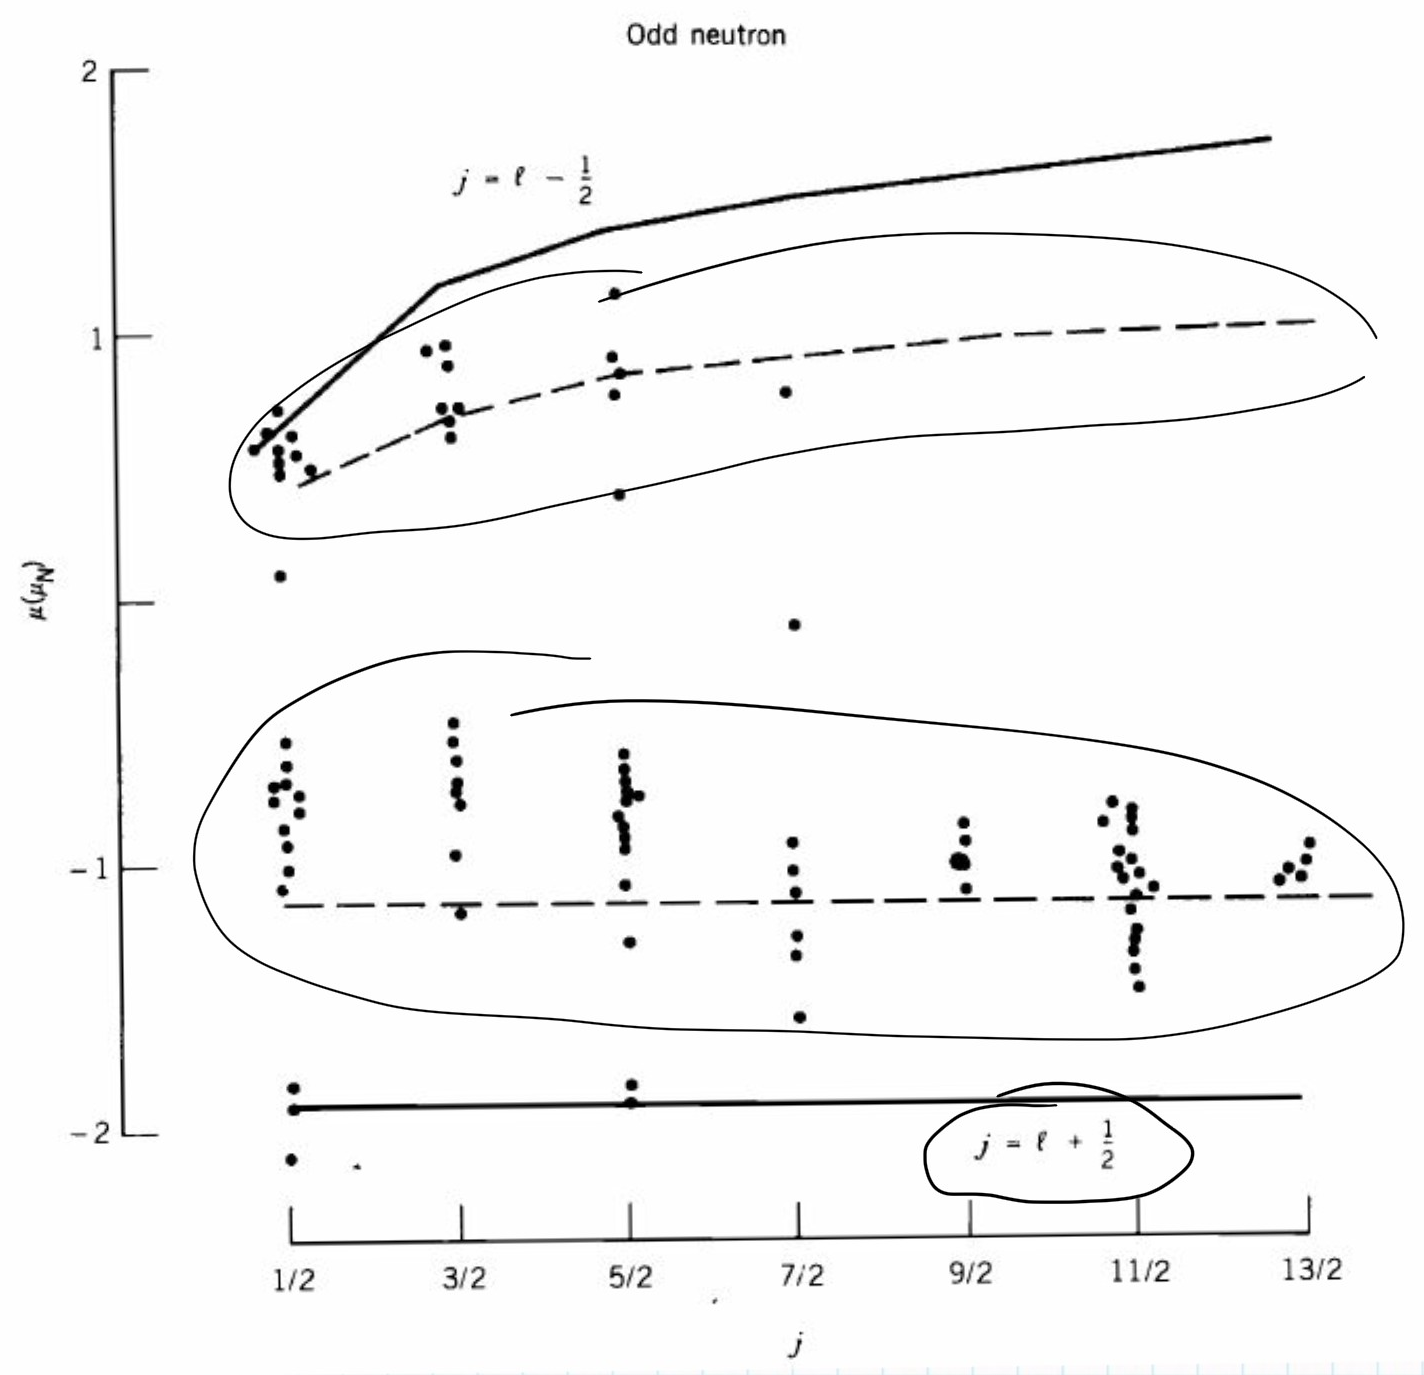
\includegraphics[scale=0.175]{Immagini/curve-Smith.png}
    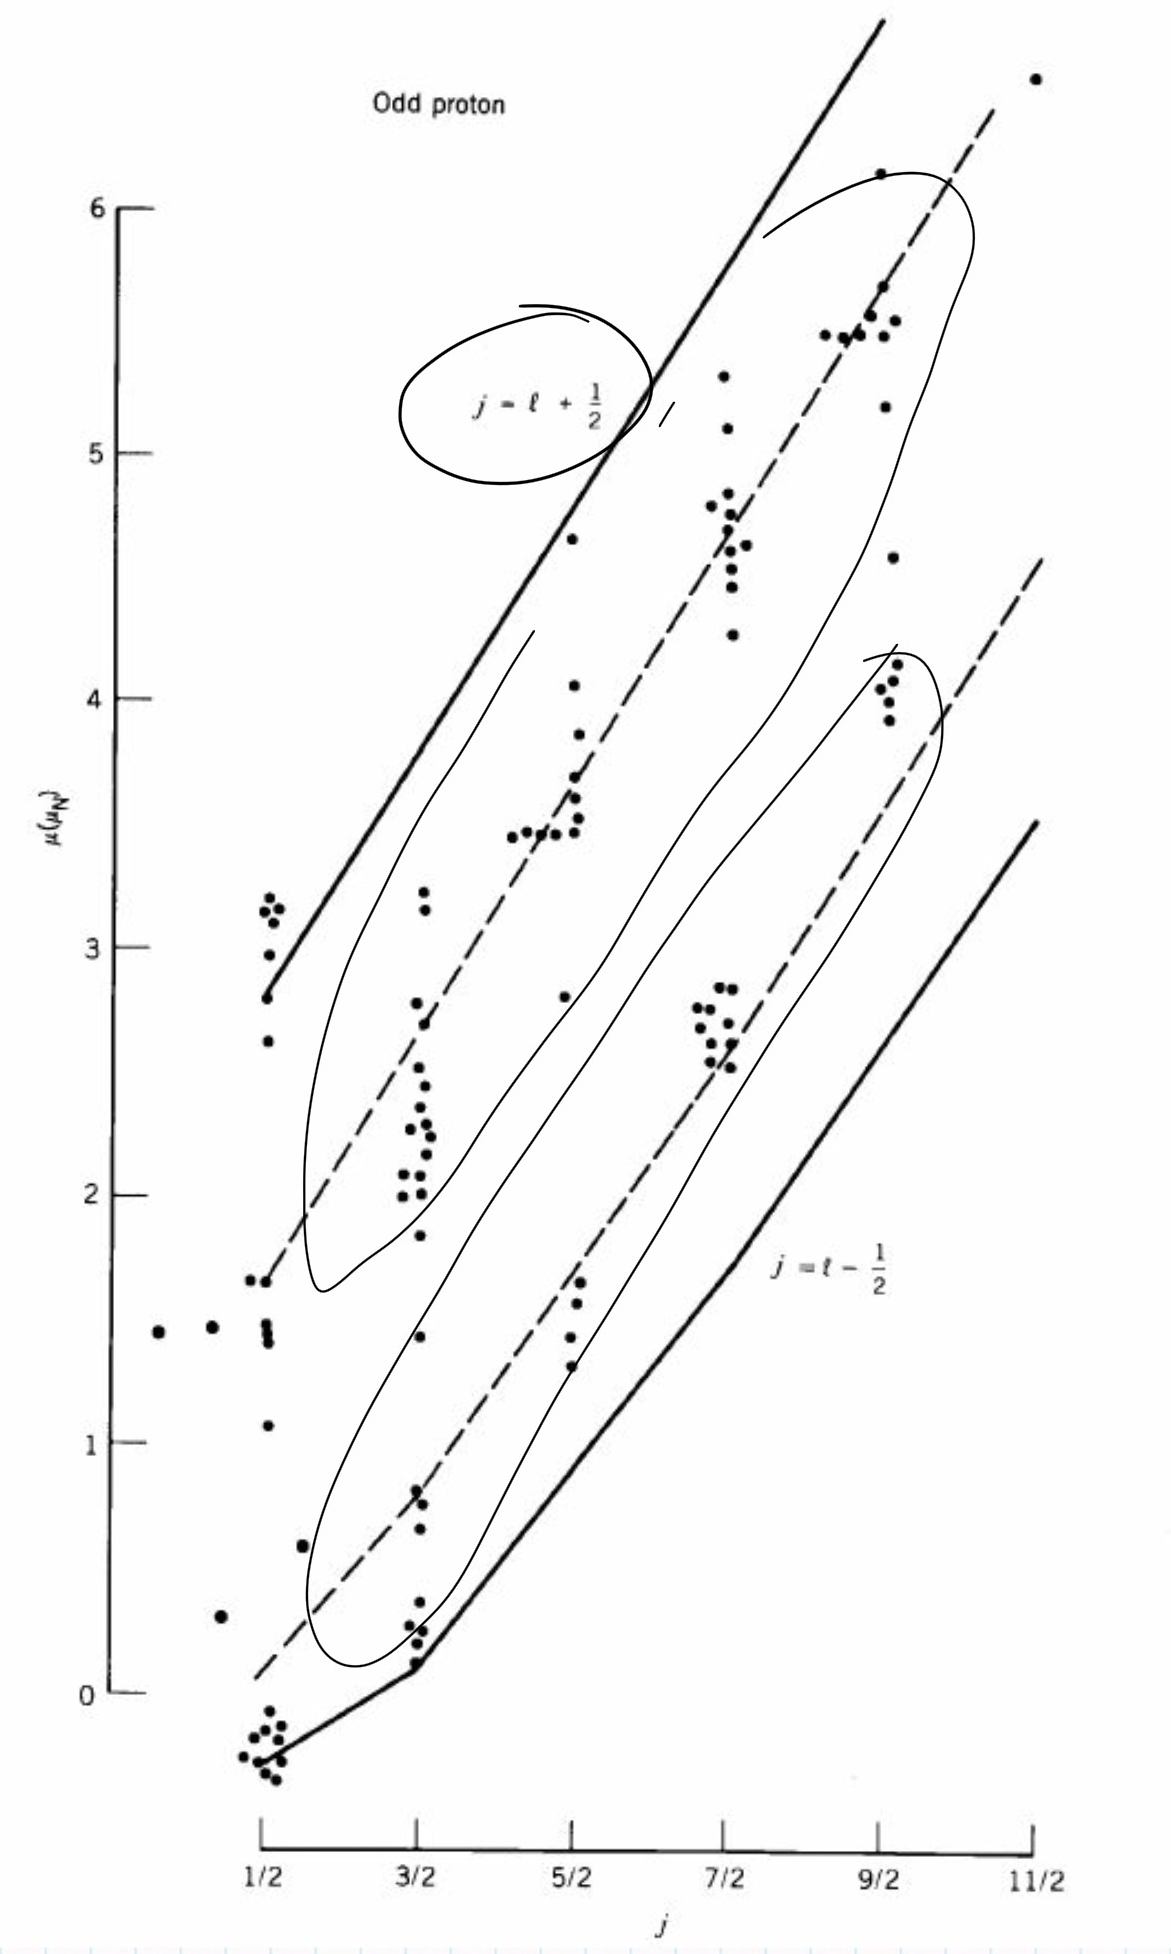
\includegraphics[scale=0.175]{Immagini/curve-Smith2.png}
    \caption{Andamenti dei momenti di dipolo magnetico per il neutrone a sinistra e per il protone a destra. La linea continua rappresenta le linee di Smith senza correzione, mentre quella tratteggiata tiene conto della \textit{medium modification}.}
    \label{curve}
\end{figure}

\begin{figure}[!h]
    \centering
    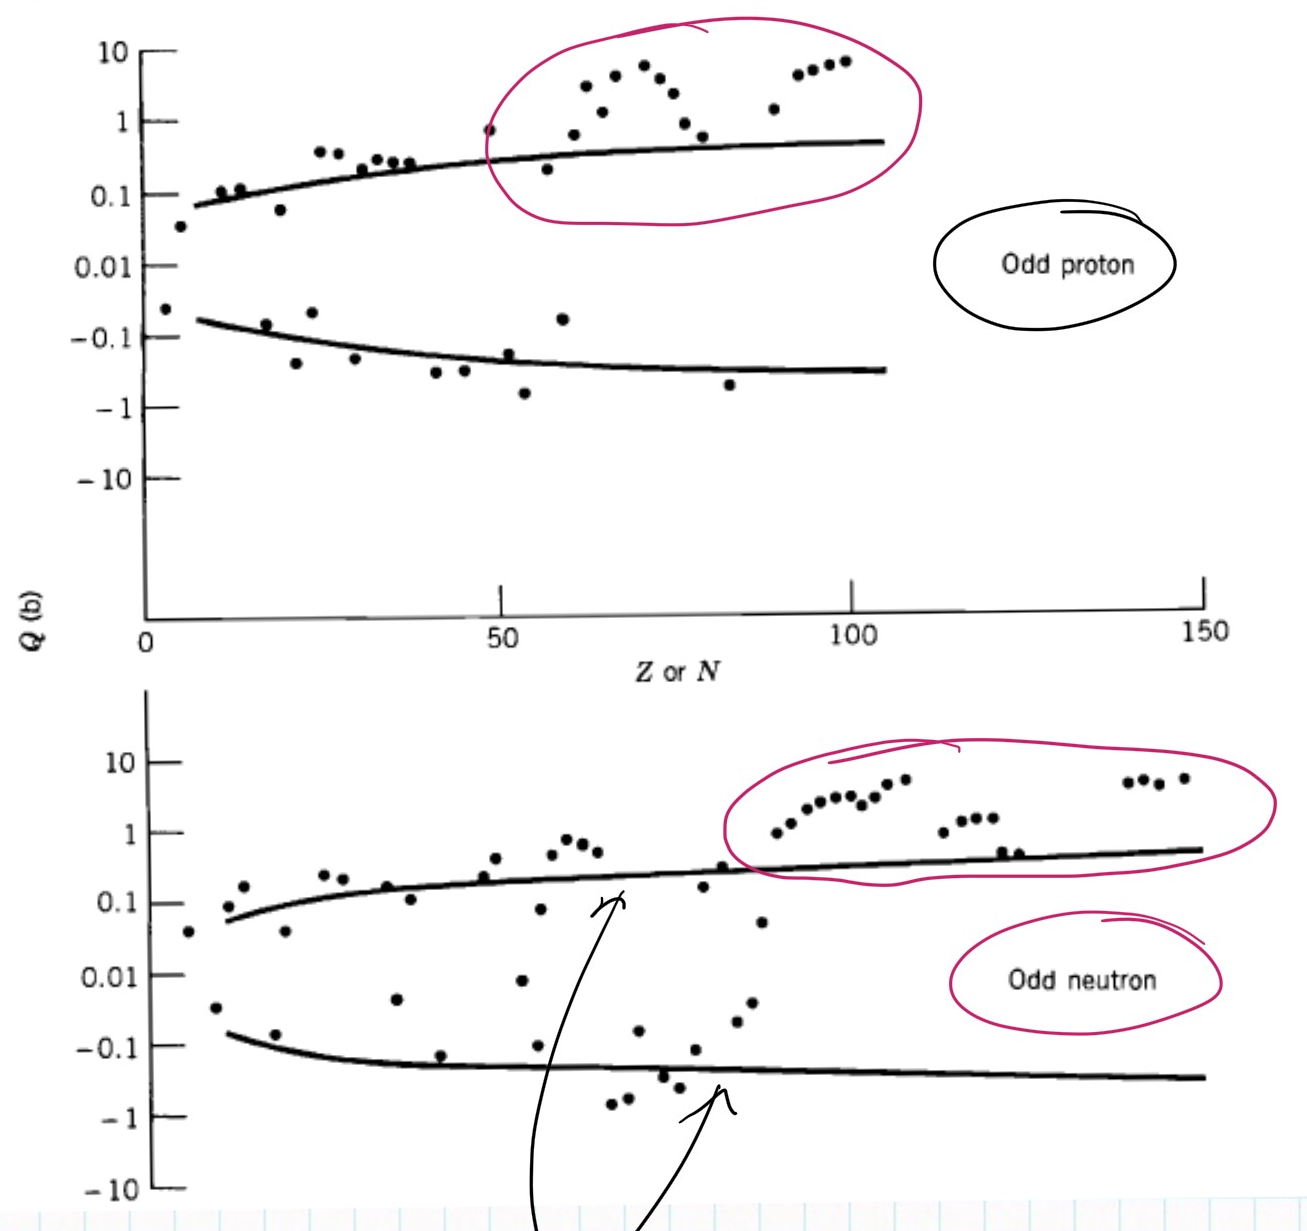
\includegraphics[scale=0.2]{Immagini/andamenti.png}
    \caption{Andamenti dei momenti di quadrupolo elettrico per il protone spaiato in alto e per il neutrone spaiato in basso.}
    \label{Q}
\end{figure}    %   01/03
%%  Modello a goccia e decadimento beta
%\part*{Lezione 03/03/2021}
\section{Modello \textit{a goccia}}
\subsection{La necessità di un nuovo modello}
Torniamo sulle problematiche del modello \textit{a shell}. Prendiamo $\ce{^{130}_{50}Sn_{80}}$: è un pari-pari per cui ci aspettiamo che lo stato fondamentale sia uno $0^+$. I problemi del modello compaiono quando cerchiamo di spiegare lo stato $2^+$ a 1 MeV dal fondamentale. Non ho protoni spaiati perché 50 è un numero magico; per quanto riguarda i neutroni, ne mancano 2 per fare il numero magico 82, allora potremmo provare a promuovere un neutrone da uno dei livelli inferiori. Tuttavia, poiché il salto dev'essere di 1 MeV non può certo venire da $1g_{9/2}$, allora supponiamo inizialmente provenga da $3s_{1/2}$: $5\leq j_{3s} + j_{1h}\leq6$, non portano ad avere un $2^+$. Anche se si prova a cercare un altro stato da cui prendere il neutrone non si riesce a trovarne uno che spieghi $J^\pi=2^+$ e il salto di 1 MeV, poiché è sempre necessario \vir{rompere} una coppia di nucleoni (circa 2 MeV). Inoltre, si osserva la presenza di questo stato (a energie minori) per ogni nucleo pari-pari con circa $150<A<200$, come in Figura \ref{graf2+}.

\begin{figure}[h]
    \centering
    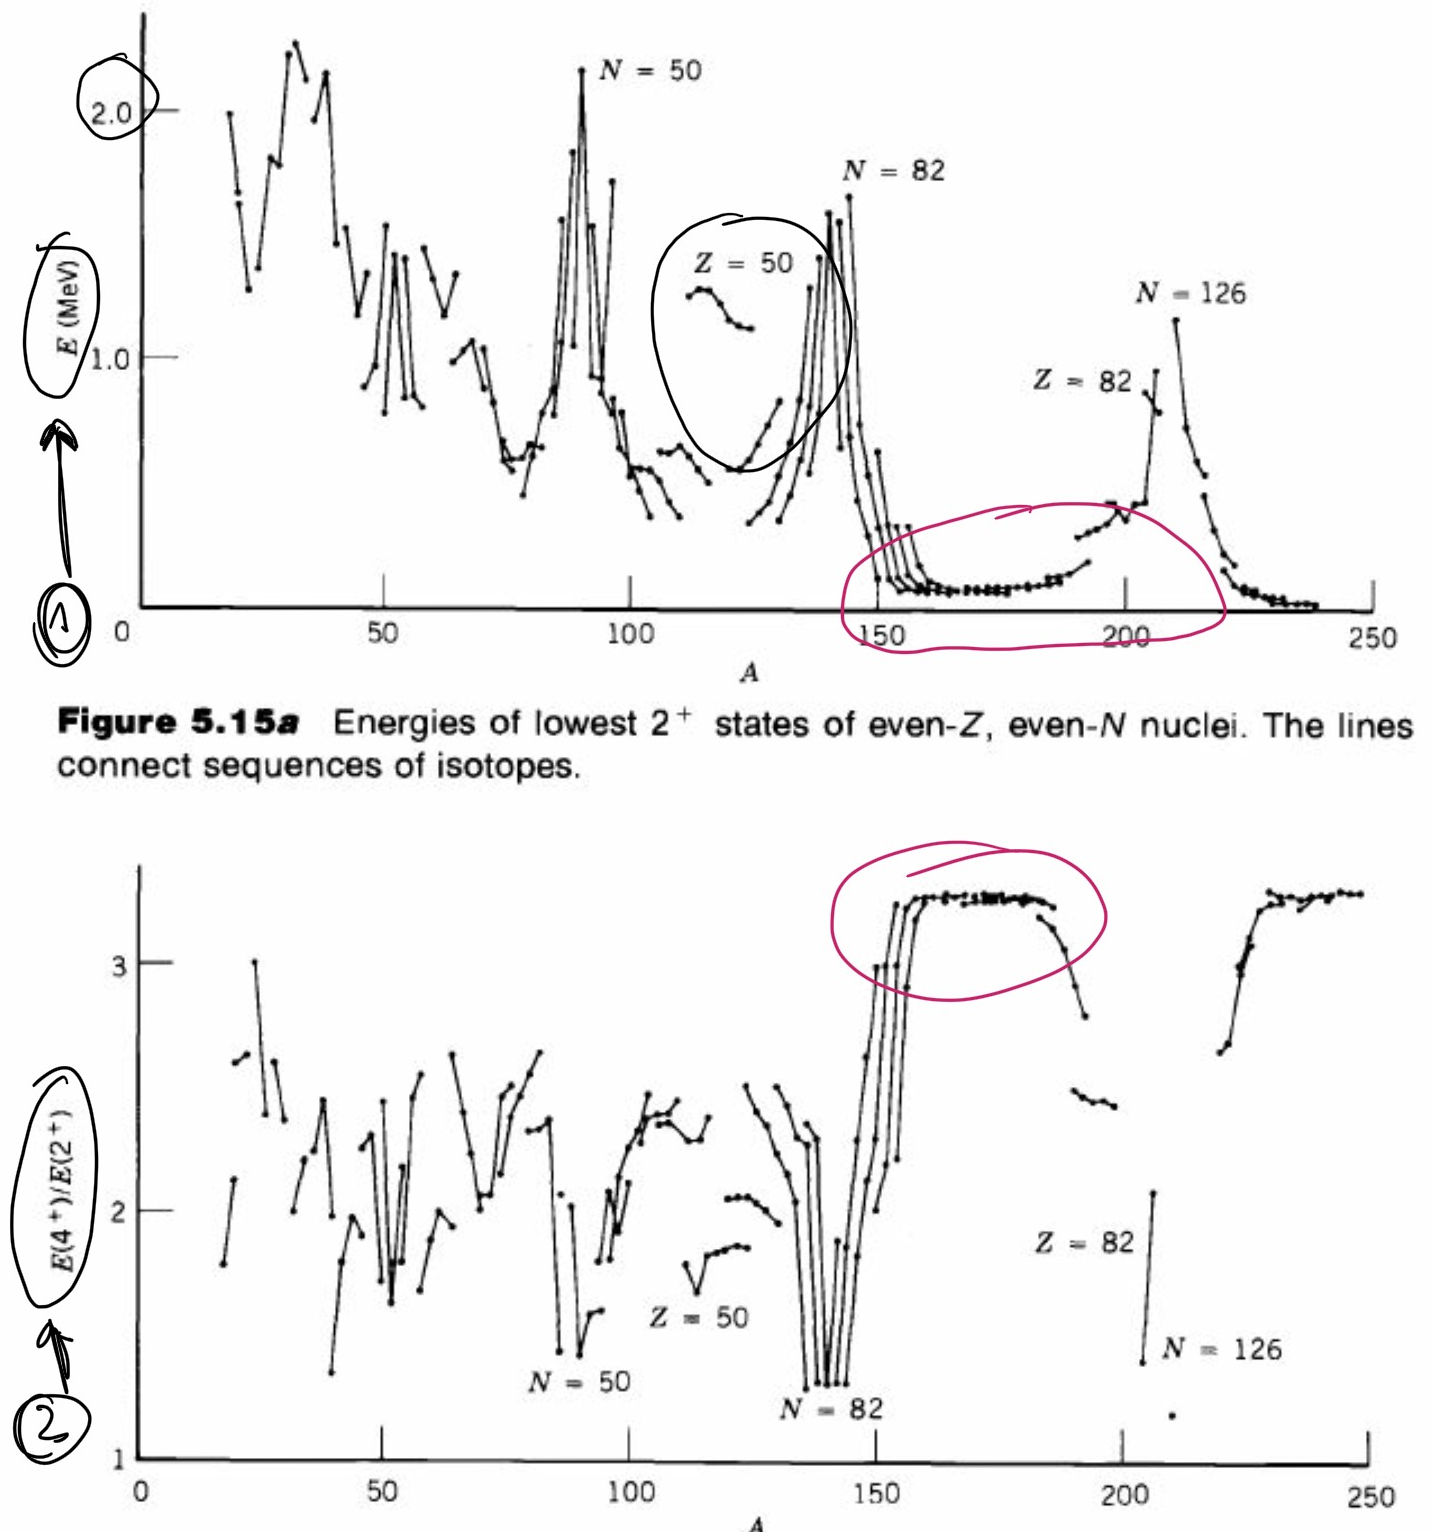
\includegraphics[scale=0.2]{Immagini/150200.png}
    \caption{In basso andamenti del rapporto tra $E(4^+)$ e $E(2^+)$ al variare $A$. Le linee non sono fit, ma collegano semplicemente i dati.}
    \label{graf2+}
\end{figure}
\begin{figure}[h]
    \centering
    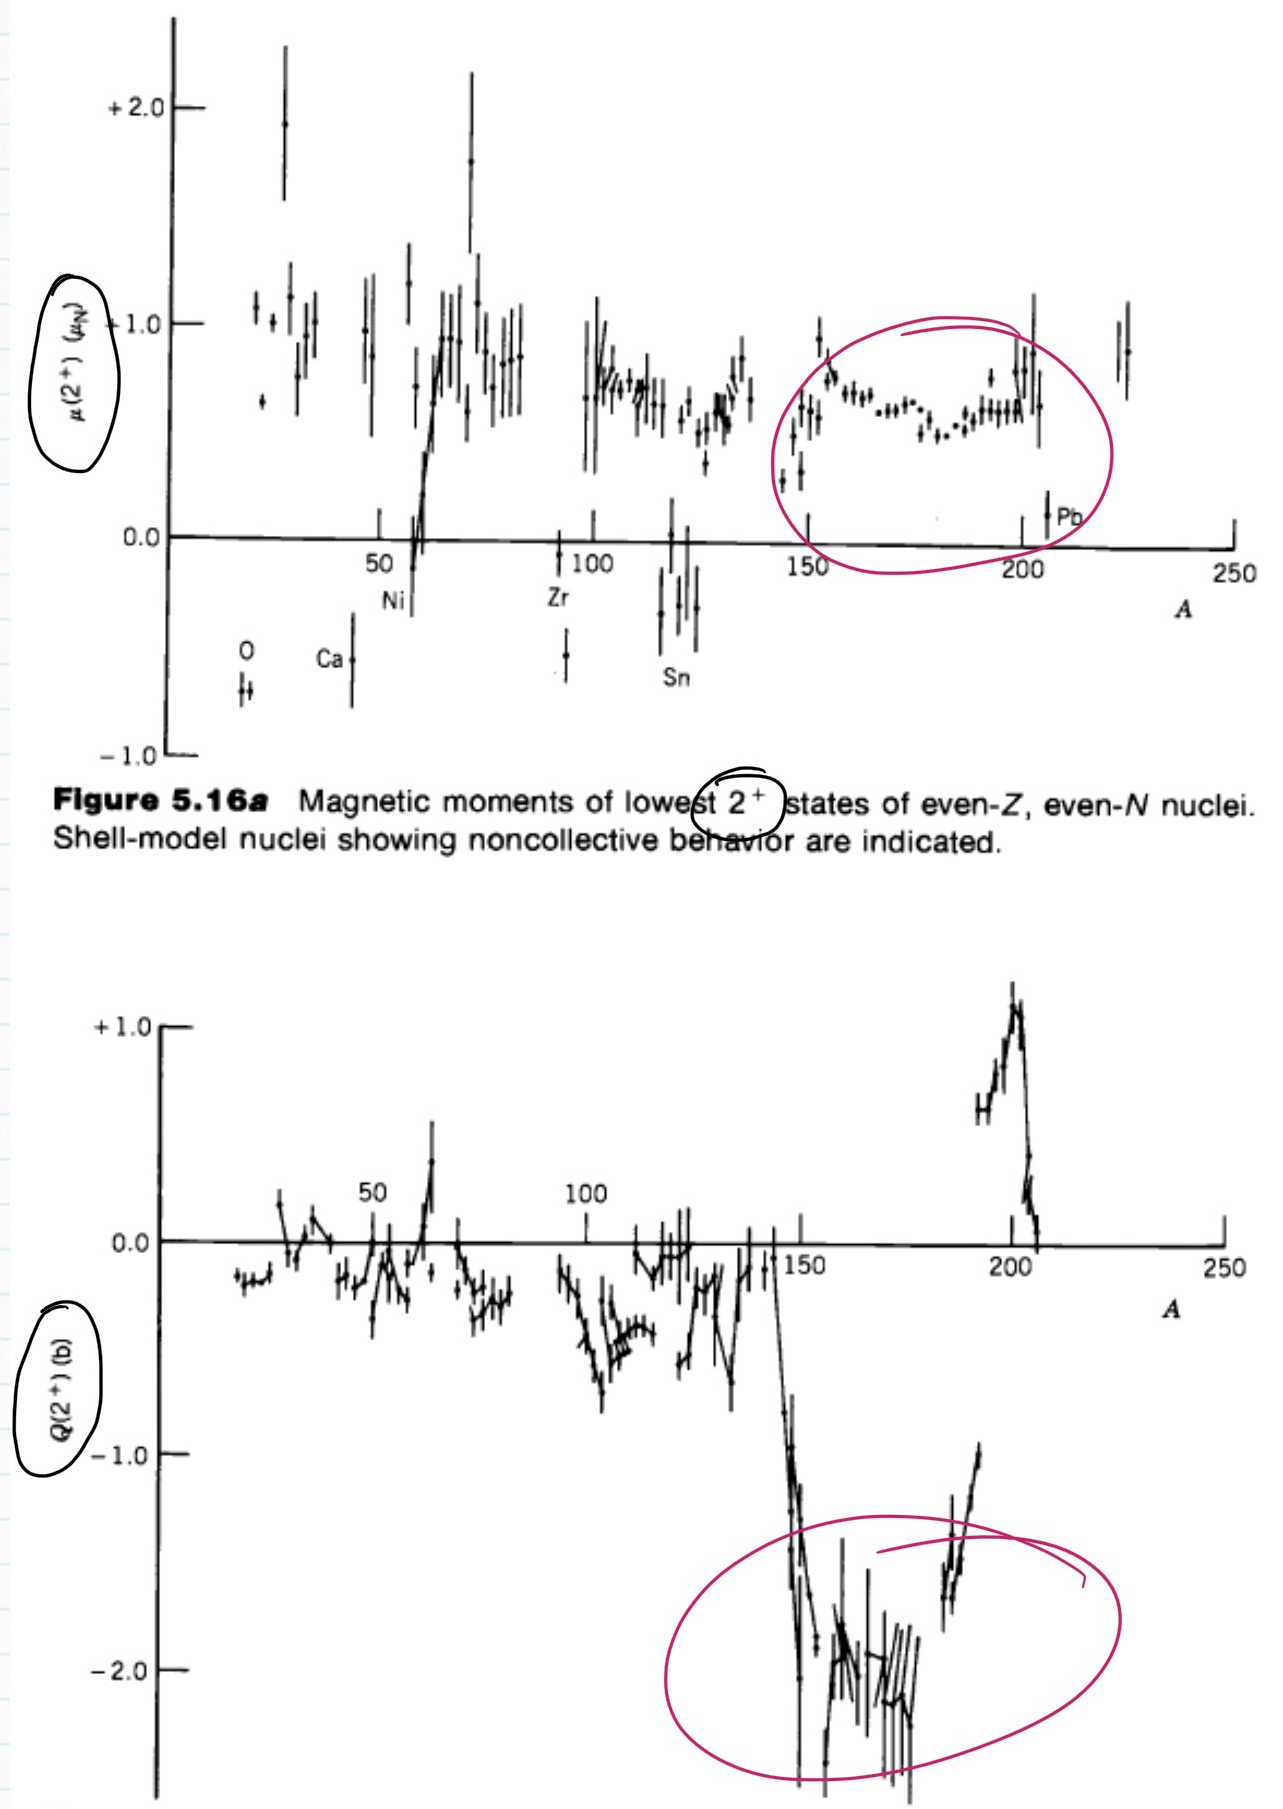
\includegraphics[scale=0.25]{Immagini/150200_2.png}
    \caption{In basso andamento del quadrupolo per lo stato $2^+$ al variare di $A$. Le linee non sono fit, ma collegano semplicemente i dati.}
    \label{graf2+1}
\end{figure}

\subsection{Stati vibrazionali}
Una spiegazione soddisfacente di tali stati eccitati e dell'andamento dei momenti di dipolo magnetico e di quadrupolo elettrico (in Figura \ref{graf2+1}), è data dal \textbf{\textit{Liquid Drop Model}}\index{modelli nucleari! a goccia@\textit{a goccia}}: assunta una configurazione sferica di equilibrio, si descrivono come \vir{vibrazioni} attorno a essa gli stati del nucleo, che a questo punto sono effettivamente stati collettivi (contrariamente al modello \textit{a shell}).\\
Pensiamo allora a una \vir{goccia} sferica che si deforma e definiamo $R(t)$ il raggio in funzione del tempo come:
$$R(t) = R_{av} + \sum_{\lambda\geq 1,\; \mu=-\lambda \dots \lambda}\alpha_{\lambda \mu}(t) \mathcal{Y}_{\lambda\mu}(\theta,\varphi)$$
con simmetria per riflessione $\alpha_{\lambda\mu} = \alpha_{\lambda\,-\mu}$, $\mathcal{Y}_{\lambda\mu}$ l'armonica sferica e $R_{av}=R_0\,A^{1/3}$ (corrispondente a $\lambda = 0$). Per $\lambda=1$ (dipolo) abbiamo una semplice traslazione del centro della sfera (vettore spostamento del $R_{CM}$), quindi non ci interessa; per $\lambda = 2$, invece, si ha $\mathcal{Y}_{2\mu}$ che è legata a un quadrupolo e quindi a una deformazione della struttura. Partendo proprio dal quadrupolo proponiamo una descrizione quantizzata degli stati vibrazionali.

\paragraph{Fononi} Possiamo allora prendere $\lambda=2 $ come unità e definire un quanto di energia vibrazionale, il \textbf{fonone}\index{fonone}, che  in questo caso prenderà il nome di fonone di quadrupolo; quindi $0^+ + $ 1 fonone $\lambda=2$, che si porta dietro $Y_{2\mu}$, $\ell =2$ e $\pi=+$:
$$0^+ + 2^+ = 2^+$$
Il $2^+$ è allora il primo stato eccitato vibrazionale del nucleo, anche se l'energia del fonone in questa trattazione è un parametro libero. Supponiamo allora di aggiungerne un altro: $\mu = \mu_1 + \mu_2$ e $\mu_i = -2, \dots, 2$, da cui $5\cdot 5 = 25$ combinazioni possibili. In realtà non è così, le combinazioni effettive sono solo 15. Guardiamo infatti la Tabella \ref{mumu}: per $\mu=4$ abbiamo una sola possibilità; per $\mu=3$ ne avremmo 2, ma dal momento che il fonone ha \textit{spin} intero la sua funzione d'onda dev'essere simmetrica, di conseguenza le possibilità si riducono a una; per $\mu = 2$ avremmo 3 possibilità, ma si riducono a 2 e così via. 

\begin{table}[!h]
    \centering
    \begin{tabular}{|c|ccccc|}
        \hline
        \multirow{3}{*}{$\mu_2$} & \multicolumn{5}{c|}{$\mu_1$} \\
        \cline{2-6}
         & -2 & -1 & 0 & 1 & 2 \\
        \hline
        -2 & -4 & -3 & -2 & -1 & 0 \\
        -1 & -3 & -2 & -1 & 0 & 1 \\
        0 & -2 & -1 & 0 & 1 & 2 \\
        1 & -1 & 0 & 1 & 2 & 3 \\
        2 & 0 & 1 & 2 & 3 & 4 \\
        \hline
    \end{tabular}
    \caption{Valori di $\mu=\mu_1+\mu_2$ per 2 fononi di quadrupolo.}
    \label{mumu}
\end{table}
\noindent Tenendo conto dello \textit{spin} del fonone, si arriva a 15 combinazioni, che possono essere descritte così:
\begin{displaymath}
\begin{aligned}
&\ell = 4 & &\mu=-4,\dots,4 & &9 \text{ Possibilità} \\
&\ell = 2 & &\mu=-2,\dots,2 & &5 \text{ Possibilità} \\
&\ell = 0 & &\mu=0 & &1 \text{ Possibilità}\\ 
\hline
& & &\text{Tripletto} & &15 \text{ Possibilità} 
\end{aligned}
\end{displaymath}
\noindent Ci aspetteremo dunque un tripletto $0^+,2^+,4^+$ degenere con energia circa il doppio di quella del $2^+$ di un solo fonone. Ci sono evidenze di questo, per esempio, nel $\ce{^{120}_{52}Te_{68}}$\footnote{Detto \textit{\vir{la perfetta goccia vibrante}}.}, dove però compaiono\footnote{Non è stato inserito il disegno dei livelli.}, oltre al $2^+$ e al tripletto, il quintetto $2^+,0^+,3^+,4^+,6^+$ (dovuto a 3 fononi) e il $3^-$ (ovvero un ottupolo $\ell=3$).

\subsection{Bande rotazionali} 
Con il modello vibrazionale abbiamo spiegato gli stati $2^+$ e $4^+$, tuttavia non abbiamo ancora chiarito i problemi per i nuclei con $150<A<200$ per quanto riguarda il loro momento di quadrupolo (molto maggiore rispetto a quello dei nuclei con $A<150$), come in Figura \ref{Q}). \\
Tali valori del momento ci suggeriscono che i nuclei siano fortemente deformati rispetto alla simmetria sferica dello $0^+$, per cui li descriviamo come ellissodi di rotazione:
$$R(\theta,\phi) = R_{av}(1+\beta\, \mathcal{Y}_{20}(\theta,\phi))$$
$$\beta = \frac{4}{3}\sqrt{\frac{\pi}{5}} \frac{\Delta R}{R_{av}}$$
dove $\Delta R$ è la differenza tra semiasse maggiore e minore e (in prima approssimazione) $R_{av}\simeq R_0 A^{\frac{1}{3}}$ è il raggio medio. In base al segno di $\beta$ si ha una figura:
\begin{itemize}
    \item \textbf{prolata}\index{figura!prolata} $\Rightarrow \; \beta >0$, Figura \ref{0303_proobl} a destra.
    \item \textbf{oblata}\index{figura!oblata} $\Rightarrow \; \beta <0$, Figura \ref{0303_proobl} a sinistra.
\end{itemize}
\begin{figure}[h]
    \centering
    \includegraphics[scale=0.7]{Immagini/0303_proobl.png}
    \caption{A sinistra figura oblata, a destra prolata. Questa immagine è stata presa da internet e non fa parte di quelle del corso.}
    \label{0303_proobl}
\end{figure}
Possiamo allora calcolare il momento di quadrupolo magnetico nel sistema di riferimento del nucleo (corotante):
$$Q_0 = \frac{3}{\sqrt{5\pi}}R^2_{av}Z\beta(1+0.16\,\beta)$$
Tuttavia, se una figura prolata ruota può apparire oblata, per cui se il nucleo ha $Q_0>0$ osserviamo un $Q<0$ nel sistema del laboraotorio e questo spiega il valore negativo del momento di quadrupolo. A titolo di esempio, riportiamo il valore per il $2^+$ (per il quale si osserva $Q\sim -2\unit{b}$):
$$-2\unit{b} \simeq Q = -\frac{2}{7} Q_0 \; \Rightarrow \; Q_0 \simeq -7\unit{b}$$
$$\beta \simeq 0.29$$
Abbiamo quindi un nucleo fortemente deformato.\\
\paragraph{Quantizzazione} Per una descrizione quantizzata di tali nuclei scriviamo l'espressione dell'energia cinetica di rotazione:
$$E_{cin} = \frac{1}{2} I \omega^2=\frac{1}{2}\frac{L(L+1)}{I}$$
dove $I=L/\omega$ è il momento di inerzia del nucleo; possiamo allora descrivere\footnote{$\ell = L/\hbar\,\Rightarrow\, E_{cin} = \hbar^2\ell(\ell+1)/2I$.} i loro stati come \textbf{bande rotazionali}\index{bande rotazionali} associate ai livelli energetici:
\begin{displaymath}
\begin{aligned}
\text{St}&\text{ato} & &E_{cin} \\
\hline
&0^+ & &0 \\
&2^+ & 6&\frac{\hbar^2}{2I} \\
&4^+ & 20&\frac{\hbar^2}{2I} \\
&\vdots & \vdots&
\end{aligned}
\end{displaymath}
\begin{figure}[h]
    \centering
    \includegraphics[scale=0.6]{Immagini/0303_liv.png}
    \caption{Livelli energetici dell'afnio.}
    \label{0303_livel}
\end{figure}
\noindent Vediamo come esempio\footnote{L'afnio è importante perché il suo decadimento viene utilizzato in fisica medica.} $\ce{^{176}_{72}Hf_{104}}$, i cui livelli\footnote{Per i calcoli abbiamo usato $\hbar^2/2I \sim 88/6 \sim 14.7$ keV} sono riportati in Figura \ref{0303_livel}:
\begin{displaymath}
\begin{aligned}
E(2^+)&= 6\frac{\hbar^2}{2I}\sim 88\, \mbox{keV} \\
E(4^+)&= 20\frac{\hbar^2}{2I}\sim 293\, \mbox{keV} \\
E(6^+)&= 42\frac{\hbar^2}{2I}\sim 621\, \mbox{keV} \\
E(8^+)&= 72\frac{\hbar^2}{2I}\sim 1064\, \mbox{keV} \\
\Rightarrow \frac{E(4^+)}{E(2^+)}&= 3.33
\end{aligned}
\end{displaymath}
L'ultimo risultato è interessante dal momento che è il valore esatto per i rapporti energetici del $\ce{^{164}_{68}Er_{96}}$. Dunque il modello riproduce con ottimo accordo le osservazioni.

%%%%%%%%%%%%%%%%%%%%%%%%%%%%%%%%%

\chapter{Decadimenti}\label{sec-decadimenti}
In questo capitolo descriveremo in modo rigoroso i decadimenti $\beta$ e $\gamma$\footnote{Per un testo di riferimento sull'argomento vedi \complrif{compl-krane}.}. Il capitolo copre le lezioni 03/03/2021, 04/03/2021, 08/03/2021 e 10/03/2021
\section{Decadimento $\beta$}
Esistono tre tipologie di \textbf{decadimento} $\beta$:
\begin{itemize}
    \item $\beta^-$: decadimento di un neutrone.
    \item $\beta^+$: decadimento di un protone.
    \item $\varepsilon$: cattura elettronica da parte di un protone.
\end{itemize}
\noindent Abbiamo quindi:
\begin{displaymath}
\begin{aligned}
&\beta^- & \ce{^A_ZX_N}&\to \ce{^A_{Z+1}Y_{N-1}} + e^- + \bar{\nu}_e & n&\to p + e^- + \bar{\nu}_e \\
&\beta^+ & \ce{^A_ZX_N}&\to \ce{^A_{Z-1}Y_{N+1}} + e^+ + \nu_e & p &\to n + e^+ + \nu_e \\
&\varepsilon & \ce{^A_ZX_N} + e^-&\to \ce{^A_{Z-1}Y_{N+1}}  + \nu_e & p+e^- &\to n + \nu_e
\end{aligned}
\end{displaymath}
dove abbiamo separato i processi nucleari da quelli base (che avvengono nel nucleo). Per capire se questi sono\footnote{Con \textit{permessi} e \textit{proibiti} si intende rispettivamente \vir{probabili} e \vir{poco probabili}.} \textit{permessi} o \textit{proibiti} è necessario calcolare il $Q$-\textit{value} $Q=\sum T_i$; possiamo momentaneamente approssimare $m_{\nu}\simeq 0$ MeV e $m_e \simeq 0.5$ MeV, ma dobbiamo considerare $m_n \not \simeq m_p$ per cui $m_n - m_p \simeq 1.3$ MeV: si osserva immediatamente che $m_n>m_p$ implica $\beta^-$ \textit{permesso} ($Q>0$) e $\beta^+$ \textit{proibito} ($Q<0$). Dunque, il protone se libero non decade\footnote{Anche in questo caso si intende che i tempi di decadimento sono \vir{lunghissimi}.}, ma può fare $\beta^+$ solo se è legato e l'energia di legame sia almeno 1.3 MeV.

\subsection{La questione dei neutrini} 
Fino al 1931, anno in cui Pauli propose l'esistenza del neutrino, i risultati dello spettro elettronico del decadimento $\beta$ furono motivo di intensa discussione: trascurando la presenza di una terza particella nei prodotti, ci si aspetterebbe un andamento del numero di elettroni in funzione dell'energia cinetica degli stessi di tipo a $\delta$, centrata sul valore del $Q$-\textit{value}\footnote{dalla conservazione dell'energia si ha appunto $m(X) = m(Y) + m_e + T_e$ per cui $Q\simeq T_e$}.
Tuttavia, quello che invece si osserva è un andamento continuo decrescente come quello riportato in Figura \ref{0303_ne}.
\begin{figure}[h]
    \centering
    \includegraphics[scale=0.5]{Immagini/0303_nume.png}
    \caption{Distribuzione del numero di neutrini in funzione dell'energia cinetica.}
    \label{0303_ne}
\end{figure}
Inizialmente, si diede come spiegazione a questo fatto la possibilità che gli elettroni prima di uscire dal campione urtassero contro altri elettroni atomici, ridistribuendo così la loro energia cinetica, ma non era esaustiva. Fu Pauli a risolvere la questione, ipotizzando per primo l'esistenza di un'altra particella non rivelata (che appunto Fermi nel 1934 chiamò \textit{neutrino}).\\ Dal calcolo del $Q$-\textit{value}:
$$Q = m_n - m_p - m_e - m_\nu \simeq 0.78 \;\mbox{MeV} - m_\nu$$
La misura di questo dà, quindi, una stima della massa del neutrino. Il problema è che è estremamente difficile da fare: i dati riportarono $Q = (0.782 \pm 0.013)$ per cui $m_\nu \simeq 0$ entro 13 keV\footnote{Con le misure più recenti si ha $m_\nu \simeq 0$ entro 1 eV}. Dunque, non è una \vir{cattiva} approssimazione quella di trascurare la massa del neutrino rispetto alle altre masse in gioco, a meno che i neutrini non siano i \vir{protagonisti} del fenomeno in esame\footnote{Vedremo in seguito un esempio in cui questo avviene.}. 
\paragraph{Q-value}\label{sec-qvalue}
Calcoliamo dunque il $Q$-\textit{value} di questi decadimenti\footnote{Procederemo in realtà al calcolo esplicito solo del decadimento $\beta^-$, poiché gli altri sono concettualmente identici.} trascurando la massa del neutrino. Definiamo la massa atomica come:
$$m_{at} (\ce{_{Z}X}) \equiv m(\ce{^A_ZX_N})+Zm_e - \sum_{i=1}^Z B_i$$
dove $B_i$ è l'energia di legame dell'$i$-esimo elettrone.
\begin{displaymath}
\begin{aligned}
Q_{\beta^-} &= m_{at}(\ce{_ZX}) - Zm_e + \sum_{i=1}^Z B_i - m_{at}(\ce{_{Z+1}Y}) + (Z+1) m_e - \sum_{i=1}^{Z+1} B_i - m_e= \\
&= m_{at}(\ce{_ZX}) - m_{at}(\ce{_{Z+1}Y}) + \sum_{i=1}^Z B_i - \sum_{i=1}^{Z+1} B_i \simeq \\
&\simeq m_{at}(\ce{_ZX}) - m_{at}(\ce{_{Z+1}Y}) \\
Q_{\beta^+} &= m_{at}(\ce{_ZX}) - m_{at}(\ce{_{Z+1}Y}) - 2m_e \\
Q_{\varepsilon} &= m_{at}(\ce{_ZX}) - m_{at}(\ce{_{Z+1}Y}) - B_n
\end{aligned}
\end{displaymath}
dove abbiamo fatto l'approssimazione $Z\sim Z+1$ poiché stiamo considerando atomi con $Z$ molto \vir{alto} e dove abbiamo definito $B_n$ la \textit{binding energy} per l'elettrone catturato dell'$n$-esimo shell\footnote{Per qualche dettaglio vedi \complrif{compl-epsilon}.} ($n = k,L,\dots$). Vediamo alcuni esempi:
\begin{displaymath}
\begin{aligned}
&\text{Decadimento} & &Q & \tau_{\frac{1}{2}}& \\
\hline
&\ce{^{23}Ne} \betamin \ce{^{23}Na} & &4.38 & 38&\,\mbox{s} \\
&\ce{^{99}Tc} \betamin \ce{^{99}Ru} & &0.29 & 2\cdot 10^5&\,\mbox{y} \\
&\ce{^{25}Al} \betaplu \ce{^{25}Mg} & &3.26 & 7.2&\,\mbox{s} \\
&\ce{^{134}I} \betaplu \ce{^{134}Te} & &2.14 & 4.2&\,\mbox{d} \\
\end{aligned}
\end{displaymath}
Dai dati sembra che non vi sia correlazione tra il $Q$-\textit{value} e il periodo di dimezzamento, che copre vari ordini di grandezza.\\
Fermi riuscì a darne una spiegazione costruendo una teoria per il decadimento.    %   03/03
%%  Teoria di Fermi sul decadimento beta e
%   decadimenti permessi e proibiti
% Tempo di dimezzamento
\newcommand{\tmez}{\tau_{1/2}}

%\part*{Lezione 04/03/2021}
\subsection{Teoria di Fermi}
Ci concentriamo sulla teoria elaborata da Fermi riguardo al decadimento $\beta$.\\
Innanzitutto, consideriamo la \textbf{regola d'oro di Fermi}\index{regola d'oro di Fermi}, definito $\lambda$ il rate di decadimento:
$$\lambda = \frac{2\pi}{\hbar} |V_{fi}|^2 \rho(E_f)$$
dove $\rho(E_f)$ è la densità degli stati finali\footnote{A volte si trova scritta come $\rho(E_f)=dn/dE_f$.} e $V_{fi} = \int d\Omega \;\psi^*_f V \psi_i$ è l'elemento di matrice\footnote{Abbiamo definito $d\Omega$ come l'elemento di volume differenziale.} dell'interazione responsabile del decadimento.\\
Fermi intuì che fosse necessario introdurre un operatore Lorentz-invariante come osservabile; questo operatore $O_X$ può essere un vettore ($_V$), un assiale ($_A$), uno scalare ($_S$), uno pseudoscalare ($_P$) o un tensore ($_T$), dev'essere l'esperimento a determinarlo e oggi sappiamo essere un vettore-assiale, comunque nella nostra descrizione lo lasceremo indeterminato. Esplicitiamo allora le funzioni d'onda:
$$V_{fi} = g \int [\phi^*_f \phi^*_e \phi^*_\nu] O_X \phi_i d\Omega$$
dove abbiamo indicato con $g$ la \textbf{costante di accoppiamento debole} o \textbf{costante di Fermi}\index{costante di accoppiamento debole@costante di accoppiamento debole $g$}\index{costante di Fermi@costante di Fermi $G_F$}. Introduciamo la notazione per i quadrimpulsi finali $p_e\equiv p $, $p_\nu \equiv q$ e $P_Y \equiv P_f$ e scriviamo i differenziali delle densità di particella:
$$\frac{dn}{dE_f} = \frac{dn_edn_\nu dn_f}{dE_f}$$
\begin{displaymath}
\begin{aligned}
&dn_e = p^2 dp d\hat{p} \frac{\Omega}{h^3} \\
&dn_\nu = q^2 dq d\hat{q} \frac{\Omega}{h^3} \\
&dn_f = P_f^2 dP_f d\hat{P_f} \frac{\Omega}{h^3} 
\end{aligned}
\end{displaymath}
Queste 3 equazioni non sono però indipendenti perché sono legate dalla conservazione del quadrimpulso ($P_f+p+q =0$), quindi se $q$ e $p$ variano si può trascurare la variazione di $dn_f$:
$$dn = \frac{p^2 dp d\hat{p}\,q^2dq\hat{q}\,\Omega^2}{h^6}$$
Per comprendere la relazione dalle direzioni $\hat{p}$ e $\hat{q}$ scriviamo le funzioni d'onda per il neutrino e per l'elettrone. Quella del neutrino essendo questo neutro ci aspettiamo sia un'onda piana $\phi_\nu = \exp{(-i\vec{q}\cdot\vec{r}_\nu/\hbar)}/\sqrt{\Omega}$; per quella dell'elettrone dovremmo considerare l'interazione coulombiana col nucleo, ma momentaneamente la trascuriamo quindi $\phi_e = \exp{(-i\vec{p}\cdot\vec{r}_e/\hbar)}/\sqrt{\Omega}$. A questo punto assumiamo l'ipotesi di Fermi, ovvero che il decadimento avvenga in un sol punto\footnote{In altre parole le particelle sono distribuite secondo $\delta(\vec{r}_\nu - \vec{r}_e)\delta(\vec{r}_e-\vec{r}_i)$ con $\vec{r}_i$ posizione del nucleone, che equivale a dire $r_e=r_\nu=r_i$.\\ 
Questa ipotesi è stata dimostrata sperimentalmente, grazie all'osservazione dei bosoni $W^\pm$ e $Z$ mediatori dell'interazione debole, che avendo una massa \vir{molto grande} hanno range di azione \vir{molto piccoli}.}, per cui utilizzeremo la sola variabile $\vec{r}$ per indicare la posizione: 
$$\int \frac{1}{\Omega} \phi^*_f e^{i\vec{p}\cdot\vec{r}/\hbar} e^{i\vec{q}\cdot\vec{r}/\hbar} O_X \phi_i d\Omega$$
A questo punto, il $Q$-\textit{value} è dell'ordine del MeV, per cui anche gli impulsi del neutrino e dell'elettrone sono di quell'ordine; inoltre le funzioni d'onda nucleari tendono a zero molto rapidamente per $r>r_{nucleare}$, dunque ci aspettiamo di poter approssimare\footnote{Questa approssimazione ha senso solo se $\phi^*_f O_X \phi_i \not = 0$.} $\phi_e\sim\phi_\nu\sim 1/\sqrt{\Omega}$. Per dare un esempio dell'ordine di grandezza dell'argomento dell'esponenziale:
$$|\frac{\vec{p}\cdot\vec{r}}{\hbar c}|\simeq \frac{1\cdot10}{200}=0.05\ll 1$$
Questa approssimazione viene detta \textbf{approssimazione a transizione \textit{permessa}}. Perché l'integrale sia non nullo allora le funzioni d'onda dei nucleoni devono avere uguale parità.\\
Riscriviamo allora il rate:
$$\lambda = \frac{2\pi}{\hbar}g^2 |\int \phi^*_f O_X \phi_i d\Omega|^2 \frac{p^2 dp 4\pi}{h^3}\frac{q^2dq4\pi}{h^3}\frac{1}{dE_f}$$
dove abbiamo integrato su $d\hat{q}$ e $d\hat{p}$ poiché niente dipende da questi. Fissiamo\footnote{In questi conti usiamo $c=1$.} l'energia dell'elettrone e del nucleone prodotto, quindi differenziamo solo in $q$, ovvero $dE_f = dE_\nu = dq$.
$$d\lambda = \frac{1}{(2\pi)^3 \hbar^7}g^2 \Bigl |\int \phi_f^* O_X \phi_f d\Omega\Bigr |^2 p^2 dp\, q^2 $$
dove $q$ è fissato da $p$. Consideriamo il numero di elettroni con impulso tra $p$ e $p+dp$: $d\lambda = N(p)dp \propto p^2 q^2 dp$. Esprimiamo $q$ in funzione dell'energia dell'elettrone tramite il $Q$-\textit{value}: $Q = T_Y + T_e + q \simeq T_e + q$ con $T_e = \sqrt{m_e^2 + p^2}-m_e$, quindi $q \simeq Q-T_e$. Abbiamo quindi:
$$N(p) \propto p^2(Q-\sqrt{m_e^2 + p^2}+m_e)^2$$
Vogliamo però esprimere tutto nell'energia cinetica dell'elettrone $dT_e = pdp/\sqrt{m_e^2+p^2}$:
$$N(T_e) \propto (Q-T_e)^2 \sqrt{(T_e+m_e)^2-m_e^2}\,(T_e + m_e) $$

\paragraph{Valutazione delle approssimazioni} In Figura \ref{0304_teo} riportiamo gli andamenti attesi per $Q\simeq 2.5$ MeV, mentre in Figura \ref{0304_dati} riportiamo i dati sperimentali. Osserviamo che l'andamento del $\beta^+$ è molto simile a quello atteso, mentre il $\beta^-$ presenta nella zona $T_e\to0$ un disaccordo con la teoria; ciò è dovuto al fatto di aver trascurato l'interazione coulombiana col nucleo, infatti il $\beta^+$ produce un positrone che è allontanato dal nucleo, mentre il $\beta^-$ produce un elettrone che risente dell'attrazione nucleare se la sua energia cinetica è \vir{bassa}.

\begin{figure}[h]
    \centering
    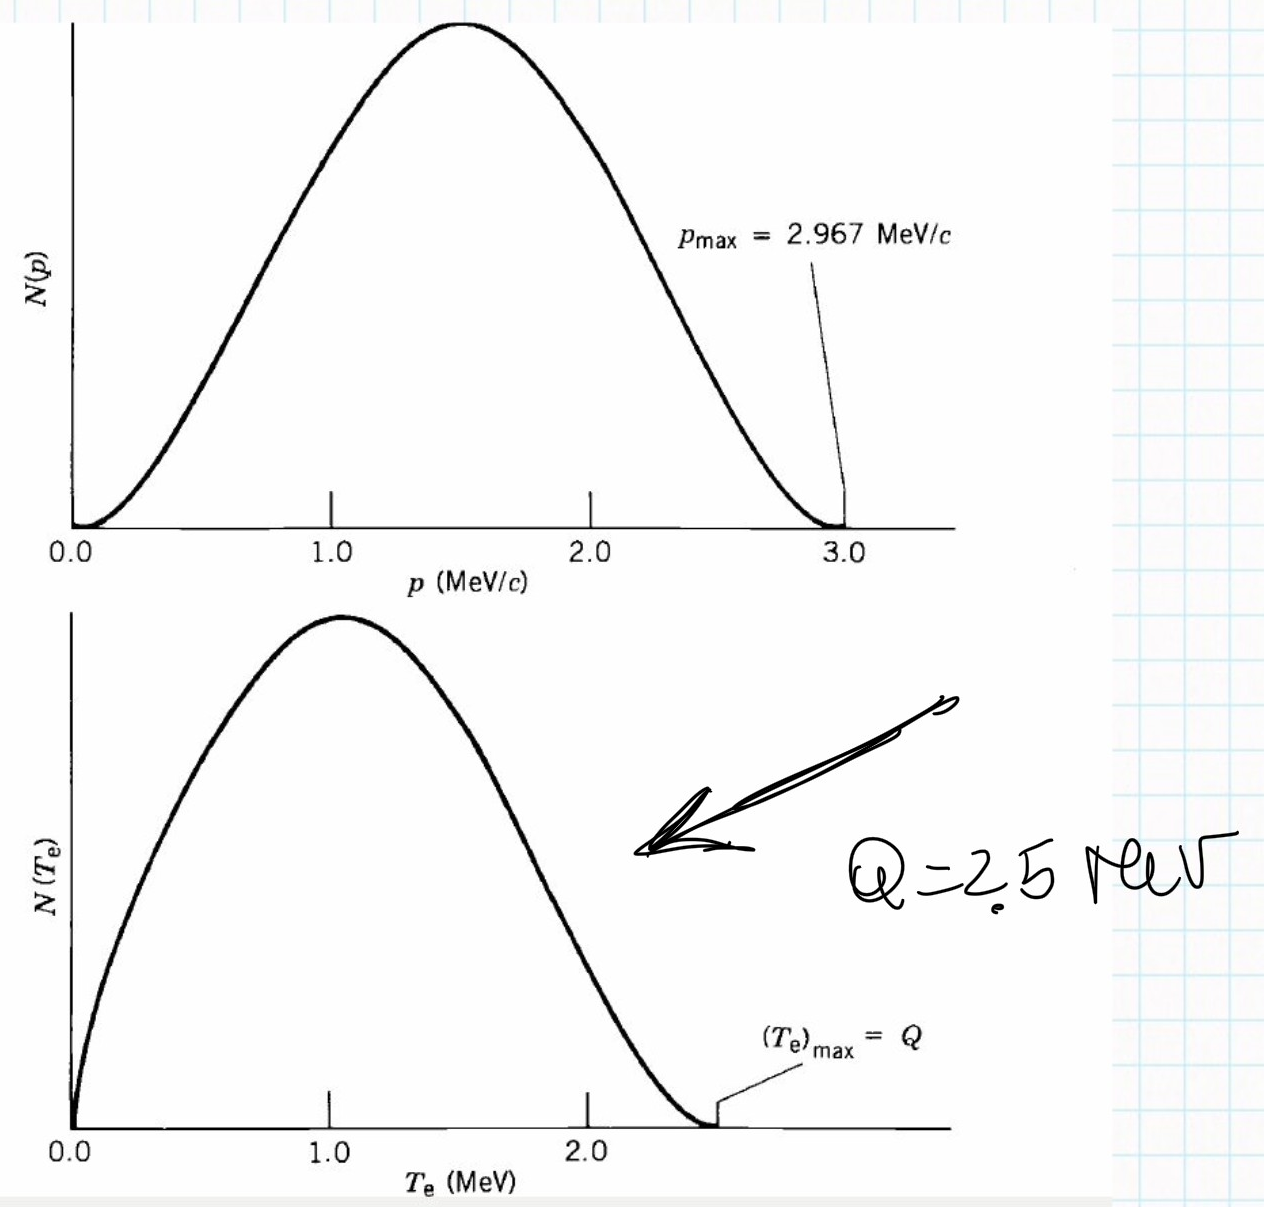
\includegraphics[scale=0.2]{Immagini/0304_andamenti.png}
    \caption{Andamenti teorici del numero di elettroni in funzione dell'impulso (in alto) e dell'energia cinetica (in basso) per il decadimento $\beta$.}
    \label{0304_teo}
\end{figure}
\begin{figure}[h]
    \centering
    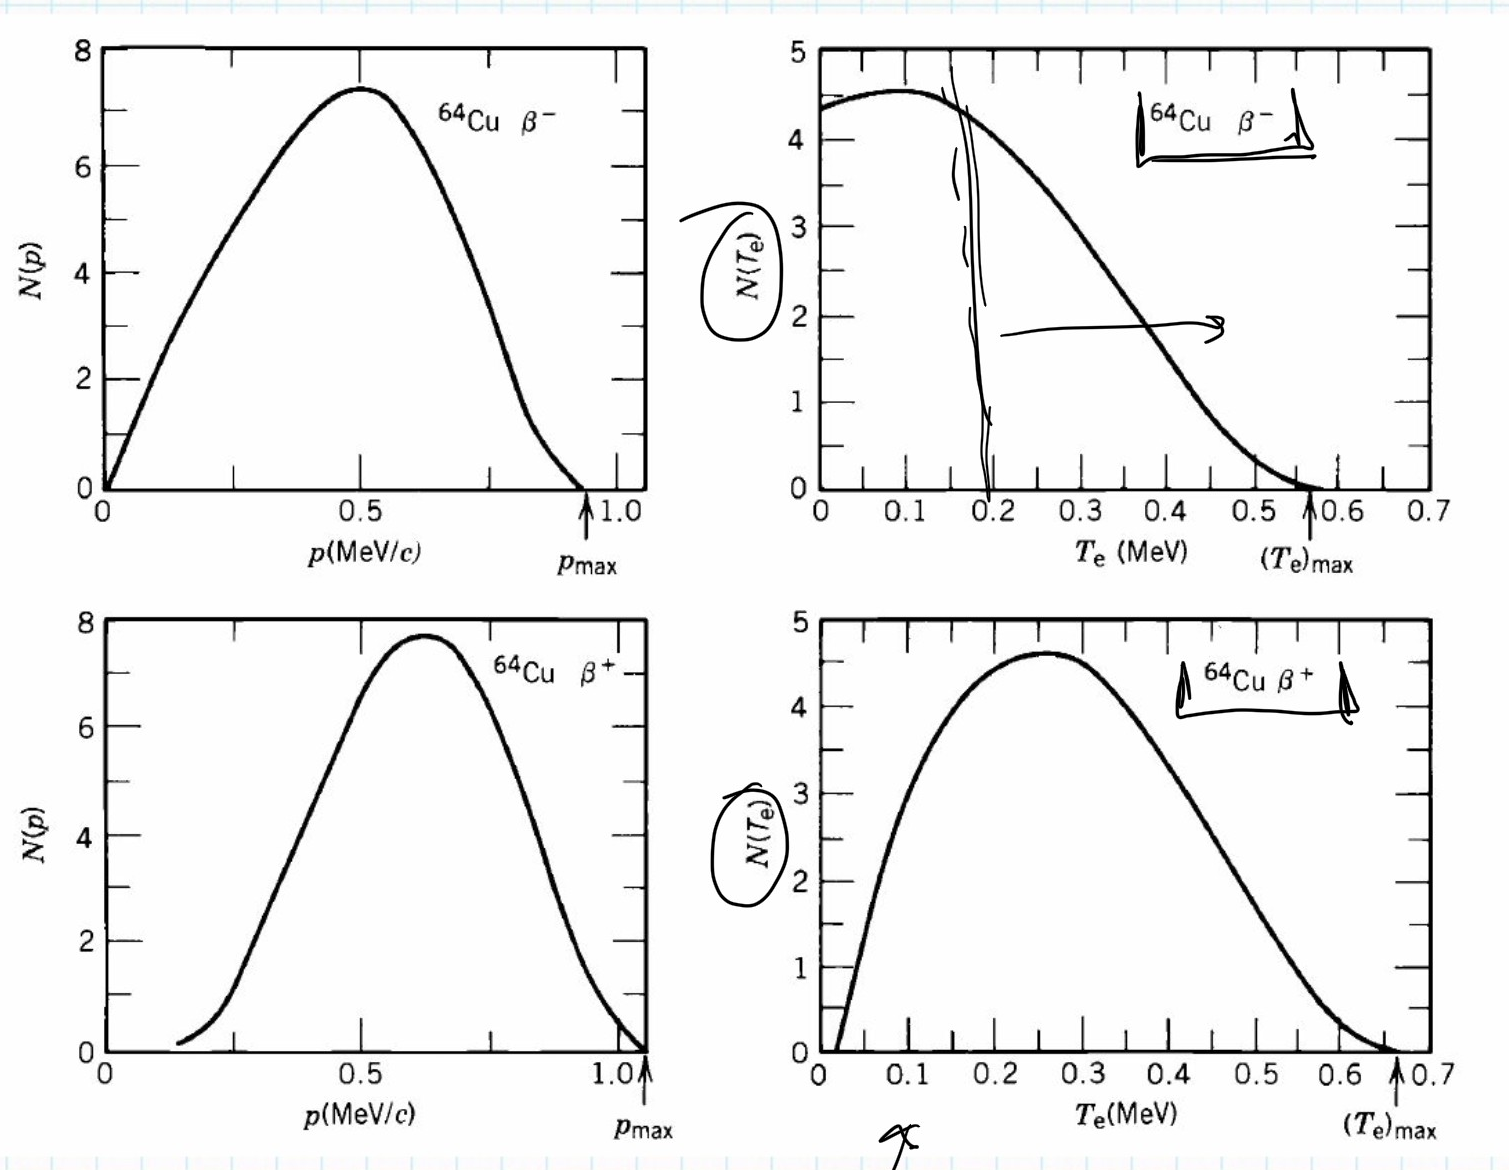
\includegraphics[scale=0.2]{Immagini/0304_andamenti2.png}
    \caption{Dati sperimentali per l'andamento del numero di elettroni nel decadimento $\beta^-$ (in alto) e nel decadimento $\beta^+$ (in basso).}
    \label{0304_dati}
\end{figure}

\noindent Fermi aveva chiaro questo e infatti non utilizzò l'onda piana per rappresentare la funzione d'onda dell'elettrone, ma un'onda distorta. Non riportiamo i calcoli di questa descrizione, ma solo il risultato:
$$N(p)\propto p^2q^2\: F(Z_Y,p)$$
dove con $F(Z_Y,p)$ si è indicato la \textbf{funzione di Fermi}\index{funzione di Fermi}, che gode della proprietà $F\to 1$ se $p\to\infty$ o $Z_Y\to0$.\\
Come già anticipato, anche l'approssimazione a transizione \textit{permessa} potrebbe essere non valida se l'operatore valutato tra gli stati iniziali e finali dei nuclei è nullo, quindi è necessario rilassarla, sviluppando in serie gli esponenziali che compaiono nelle funzioni d'onda del neutrino e dell'elettrone\footnote{Questo comporta che nell'integrazione successiva comparirà una dipendenza dalle direzioni $\hat{p}$ e $\hat{q}$, quindi dovremo tenerne conto quando si integra nell'angolo solido.}. Queste transizioni vengono chiamate \textbf{transizioni \textit{proibite}}\footnote{Come avevamo già spiegato, con \textit{proibite} non si intende \vir{non-permesse}, bensì che il tempo di decadimento è molto \vir{lungo} (dal momento che $\lambda$ è minore di quelle \textit{permesse}) e quindi l'osservazione è particolarmente difficile e rara.} e le loro approssimazioni prendono il nome dall'ordine al quale ci si ferma\footnote{Nell'espansione abbiamo trascurato i fattori costanti come $\Omega^{-1/2}$ e $\hbar^{-1}$.}:
$$\phi_\nu^* \simeq \underbrace{1}_\text{permessa}+\underbrace{i\vec{q}\cdot \vec{r}}_\text{I proibita}-\frac{1}{2}\underbrace{(\vec{q}\cdot \vec{r})^2}_\text{II proibita}+\dots$$
Considerando tutto abbiamo allora:
$$N(p)\propto p^2(Q-T_e)^2 F(Z_Y,p)\Bigl |M_{fi}\Bigl |^2 S(p,q)$$
dove abbiamo definito $M_{fi}\equiv \int \frac{1}{\Omega} \phi^*_f e^{i\vec{p}\cdot\vec{r}/\hbar} e^{i\vec{q}\cdot\vec{r}/\hbar} O_X \phi_i d\Omega $ e $S(p,q)$ lo \textbf{shape factor}\index{fattore di forma} che tiene conto dell'integrazione sull'angolo solido (quindi in $d\hat{q}$ e $d\hat{p}$) e vale 1 se la transizione è \textit{permessa}.\\
Possiamo allora esprimere $(Q-T_e)^2$ come:
$$(Q-T_e)^2\propto\frac{N(p)}{F(Z_Y,p)p^2 S(p,q)}$$
e osservarne l'andamento nel \textbf{grafico di Fermi-Kuree}\index{grafico di Fermi-Kuree} in Figura \ref{0304_qvalue} per il decadimento $0^+\to0^+$ del $\ce{^{66}Ga}$ che è un \textit{super-permesso}. Possiamo notare che per un certo valore dell'energia non vi è più accordo tra teoria ed esperimento, ciò è dovuto all'interazione dell'elettrone con sorgenti radioattive.\\
Guardiamo, invece, lo stesso grafico per una transizione \textit{proibita} del $\ce{^{91}Y}$ in Figura \ref{0304_qvalue2} e osserviamo l'accordo tra i dati e il modello senza considerare lo shape factor e con lo shape factor.

\begin{figure}[h]
    \centering
    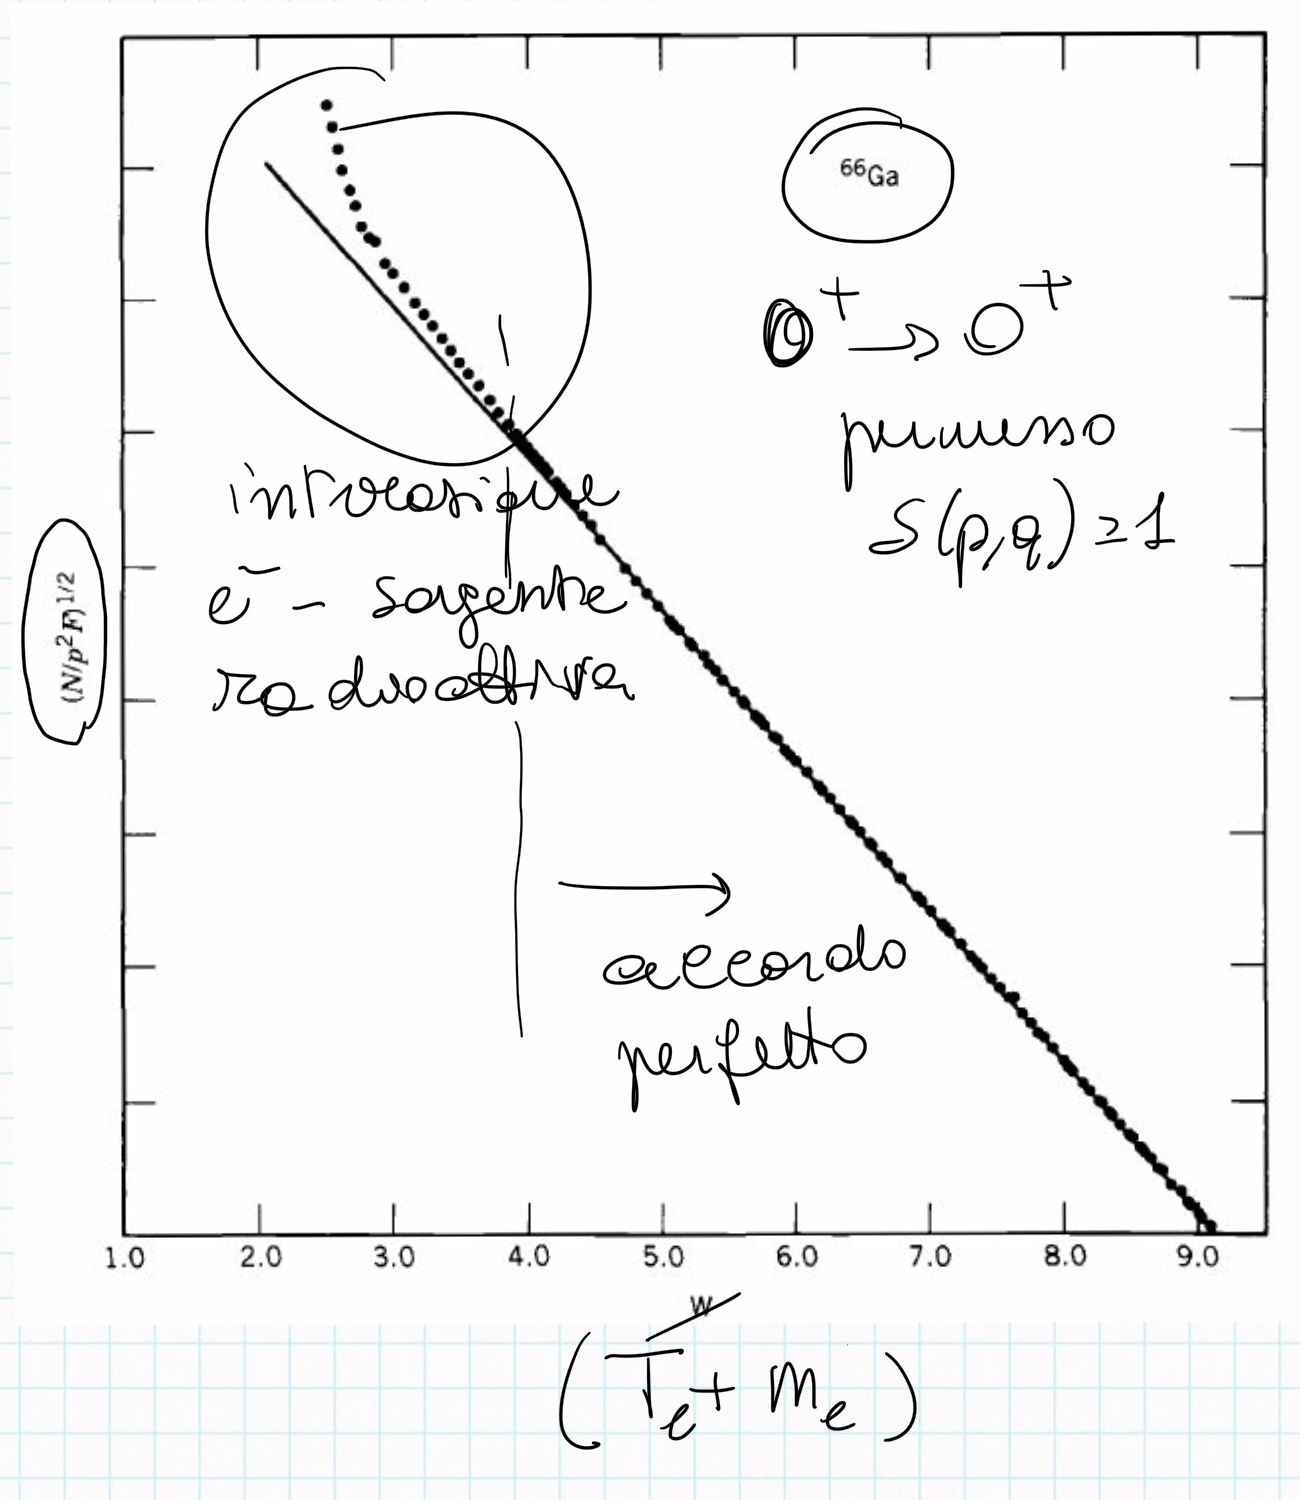
\includegraphics[scale=0.2]{Immagini/0304_andamenti3.png}
    \caption{Grafico di Fermi-Kuree che mostra l'andamento di $(Q-T_e)^2$ in funzione dell'energia dell'elettrone per il decadimento $0^+\to0^+$ del $\ce{^{66}Ga}$ e l'accordo tra i dati e il modello.}
    \label{0304_qvalue}
\end{figure}
\begin{figure}[h]
    \centering
    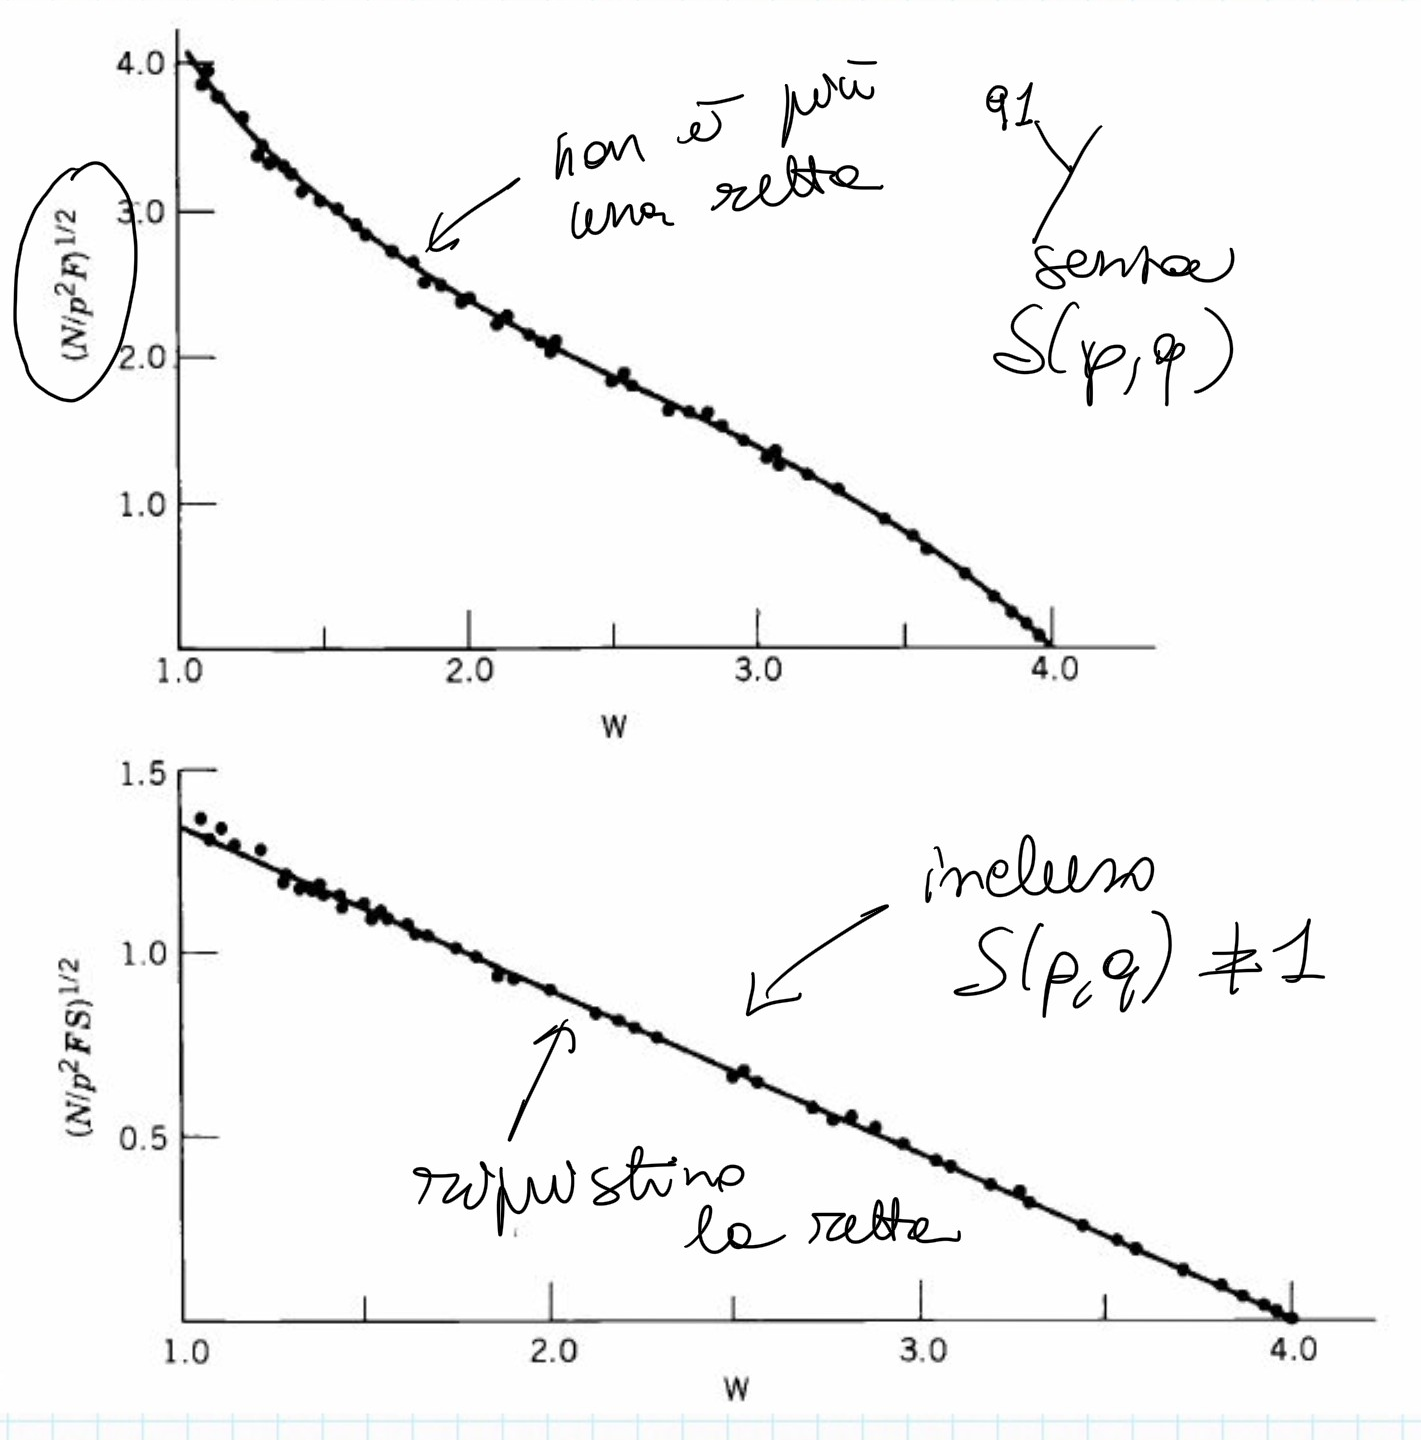
\includegraphics[scale=0.2]{Immagini/0304_andamenti4.png}
    \caption{Grafico di Fermi-Kuree che mostra l'andamento di $(Q-T_e)^2$ in funzione dell'energia dell'elettrone per il decadimento del $\ce{^{91}Y}$ e l'accordo tra i dati e il modello senza shape factor (in alto) e con shape factor (in basso).}
    \label{0304_qvalue2}
\end{figure}

\paragraph{Calcolo del rate} Abbiamo tutti gli strumenti quindi per proseguire con il calcolo del rate\footnote{Per semplicità considereremo un decadimento permesso, ovvero $S(p,q)=1$.}:
$$\lambda = \frac{g^2 |M_{fi}|^2}{2\pi^3 \hbar^7}\int_0^{p_{\max}} p^2 (Q-T_e)^2 F(Z_y,p) dp $$

\begin{definition}[\textbf{Integrale di Fermi}]\index{integrale di Fermi}
$$f(Z_Y,E_0) = \frac{1}{m_e^5 c^5}\int_0^{p_{\max{}}} p^2 F(Z_Y,p)(E_0-E_e)^2 dp$$
non è un integrale analitico, ma è tabulato per vari $Z_Y$.
\end{definition}
\noindent Per definizione di tempo di dimezzamento $\tmez$ si ha:
\begin{displaymath}
\begin{aligned}
\lambda = \frac{g^2 |M_{fi}|^2}{2\pi^3 \hbar^7} m_e^5\, f(Z_Y,E_0) &= \frac{\ln{2}}{\tmez} \\
f\tmez &= \ln{2}\frac{2\pi^3 \hbar^7}{ g^2 |M_{fi}|^2 m_e^5 c^4} 
\end{aligned}
\end{displaymath}
dove abbiamo inizialmente trascurato $c$ e poi reintrodotta. Quest'ultima espressione viene detta $f\tau$\textbf{-value}\index{ft-value@$f\tau$\textbf{-value}}, dipende solo da $|M_{fi}|$, ovvero solo dai nuclei, e varia in un range esteso tra $10^3$ e $10^{20}$ s, per questa ragione spesso se ne esprime il logaritmo. Per $\log{(f\tau)}\sim 3 \div 4$, ovvero decadimenti molto veloci, si parla di decadimenti \textit{super-permessi} e sono tutti $0^+\to0^+$ con $M_{fi}\sim \sqrt{2}$ indipendente dal nucleo considerato. Questo decadimento è allora perfetto per stimare la costante di accoppiamento debole $g$ dal momento che presenta per ogni nucleo lo stesso valore $f\tau$, come riportato in Figura \ref{0304_dati2}; si ottiene così:
$$g\simeq 0.88\cdot 10^{-4} \;\mbox{MeV}\,\mbox{fm}^3$$
Per avere una quantità adimensionale possiamo definire una costante tipica dell'interazione $G = g \,m^2c/\hbar^3$, per cui:
\begin{displaymath}
\begin{aligned}
&\text{Forte } \pi-N & &1 \\
&\text{E.M. } & &10^{-2} \\
&\text{Debole } & &10^{-5} 
\end{aligned}
\end{displaymath}
In quest'ultimo caso viene detta \textbf{costante di Fermi} $G_F$\index{costante di Fermi}.

\begin{figure}
    \centering
    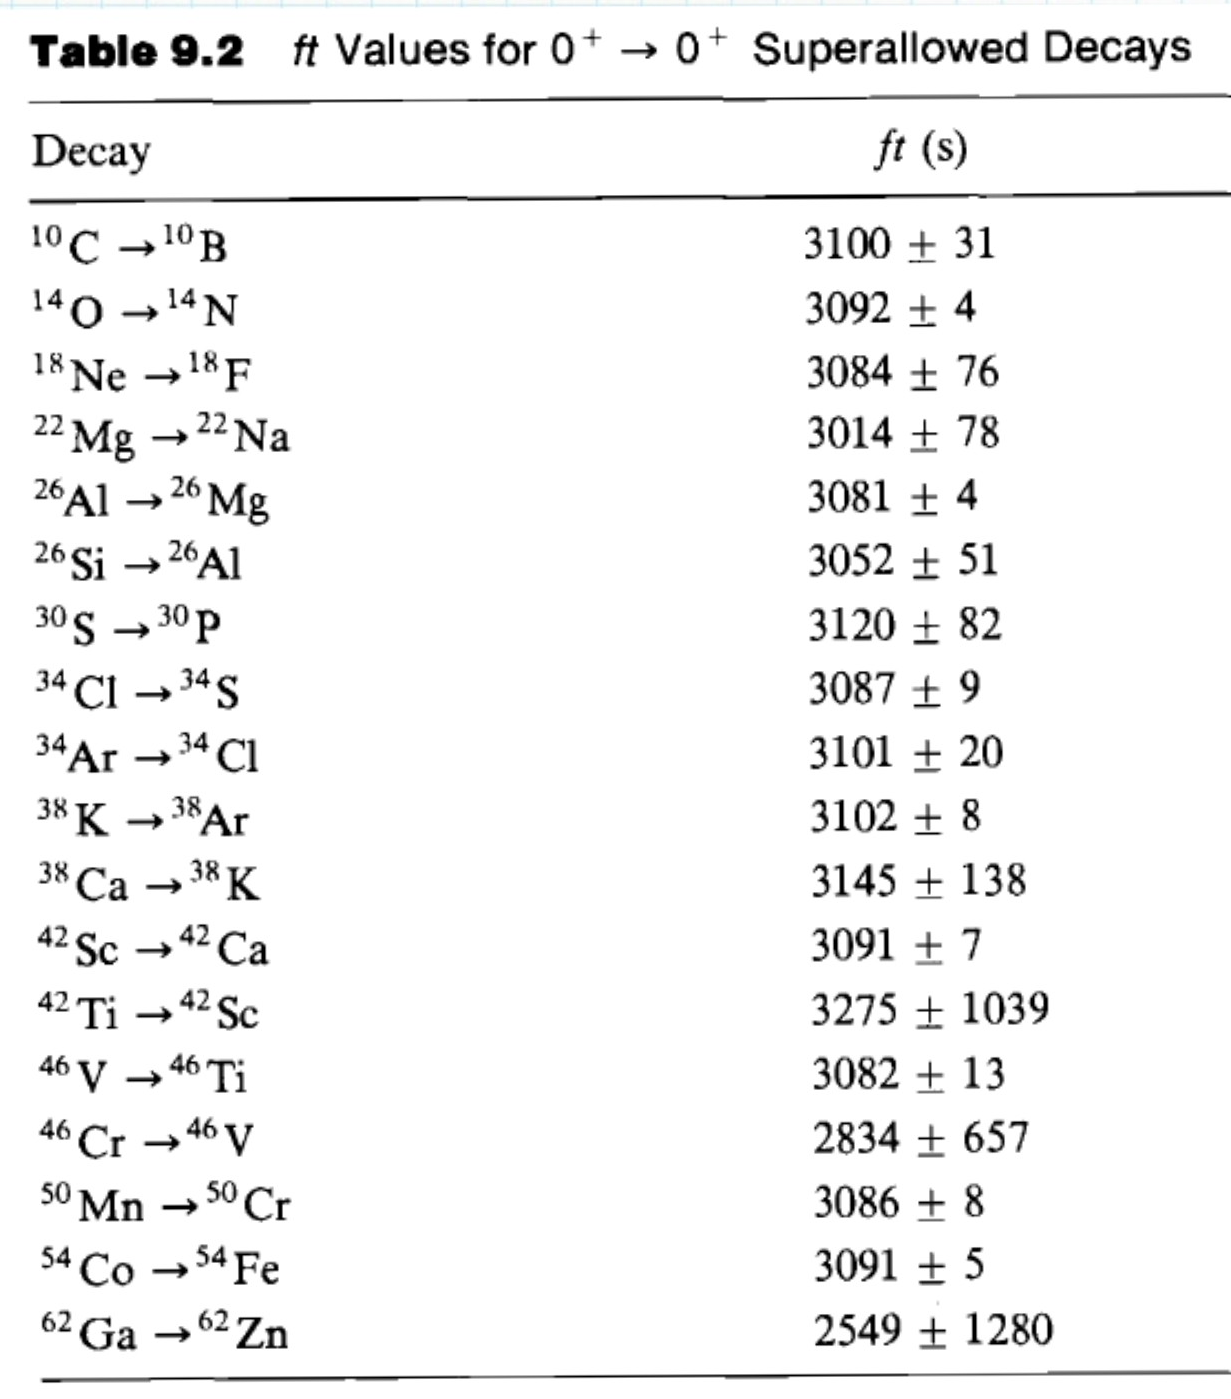
\includegraphics[scale=0.2]{Immagini/0304_dati.png}
    \caption{Tabella con la misura del $f\tau$-value per il decadimento $0^+\to0^+$ di alcuni nuclei.}
    \label{0304_dati2}
\end{figure}

\subsubsection{La massa del neutrino}
Finora per tutti i conti che abbiamo fatto, abbiamo considerato $m_\nu=0$, ma questo non è sempre un'approssimazione corretta: per elettroni energetici, ovvero $T_e\to Q$, dalla conservazione dell'energia si ha che $q\ll 1$, quindi il neutrino non è più relativistico ($q\not = Q-T_e$) e gli effetti della sua massa non sono più trascurabili\footnote{Posto $c=1$.} $E_\nu \simeq m_\nu + q^2/2m_\nu$. Poiché ciò influisce sul numero di elettroni, Fermi rielaborò i suoi conti tenendo conto della massa del neutrino e ottenne un andamento come quello riportato in Figura \ref{0304_nu}.

\begin{figure}[h]
    \centering
    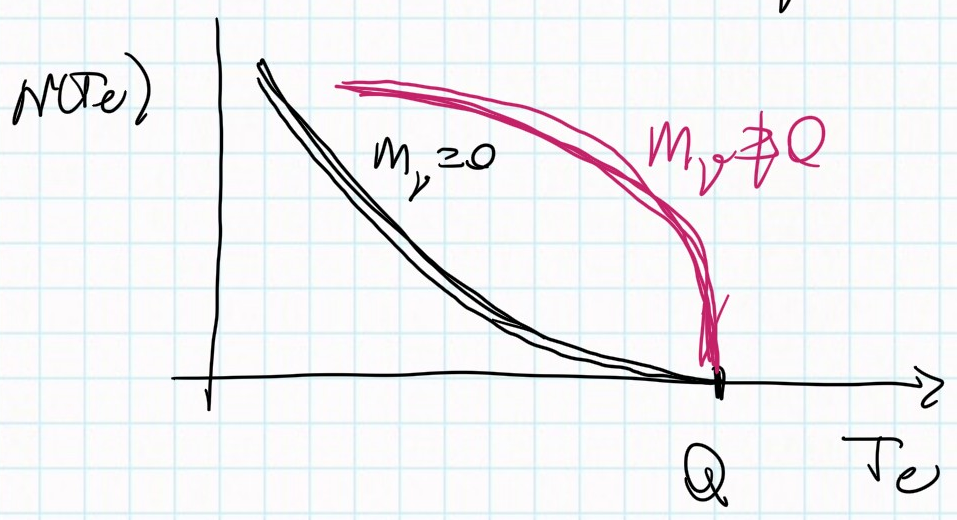
\includegraphics[scale=0.3]{Immagini/0304_neutrini.png}
    \caption{Nel grafico sono rappresentati gli andamenti del numero di elettroni in funzione dell'energia cinetica dell'elettrone senza considerare la massa del neutrino e tenendone conto. Le due curve non sono in scala.}
    \label{0304_nu}
\end{figure}

\paragraph{Esperimenti per $m_\nu$} Ci sono vari esperimenti che cercano di misurare la massa del neutrino; ne discutiamo 2:
\begin{itemize}
    \item \textbf{Katrin}\esperimento{Katrin}: in questo esperimento si sfrutta il decadimento $\beta^-$ del trizio
    $$\ce{^3H}\to\ce{^3He} + e^- +\bar{\nu}_e$$
    In questo modo è possibile misurare direttamente la massa del neutrino, ma proprio per questo è particolarmente difficile.
    \item \textbf{Ptolemy}\esperimento{Ptolemy}: si tratta in realtà di un esperimento ancora in progettazione che prevede di osservare una cattura neutrinica del trizio con neutrini lenti.
    $$\nu_e + \ce{^3H}\to\ce{^3He} + e^-$$
    Poiché $T_\nu\sim 0$ l'energia dell'elettrone è ben fissata (non è più uno spettro continuo), quindi $T_e = m(\ce{^3H}) - m(\ce{^3He}) -m_e +m_\nu $ e dal momento che il trizio decade $\beta^-$ si avrà anche $Q^\beta = m(\ce{^3H})-m(\ce{^3He})-m_e-m_\nu$, da cui:
    $$T_e = Q^\beta + 2m_\nu$$
    Ci aspettiamo quindi di osservare un andamento come quello in Figura \ref{0304_nu} dove però compare anche una $\delta$ a distanza $2m_\nu$ da $Q^\beta$. Questa misura permetterebbe quindi di ottenere una stima per $m_\nu$ e sarebbe un'evidenza sperimentale del \textbf{cosmic neutrino background}, dal quale ci si aspetta neutrini con $T_\nu\sim0 $ (quindi quelli della cattura).\\
    Questa è, però, anche una della maggiori difficoltà dell'esperimento, ovvero non ci sono ancora state evidenze di questo fondo di neutrini, quindi ci aspettiamo pochissimi eventi; inoltre \vir{immobilizzare} il trizio non è un problema banale, infatti anche se portato a 0 K questo decade molto facilmente $\beta^-$, per cui è stato proposto di legarlo al grafene (o strutture reticolari particolari) in modo da smorzare possibili movimenti.
\end{itemize}

\section{Decadimenti $\beta$ \textit{permessi} e \textit{proibiti}}
Prima di procedere con lo studio di altri decadimenti ci soffermiamo un attimo sulla probabilità di decadimento $\beta$.

\paragraph{Decadimenti permessi} Per questo tipo di decadimenti abbiamo visto che $S(p,q)=1$ da $\phi_e\sim\phi_e\sim1$, per cui $e^\pm$ e $\nu$ sono centrati in $r=0$, ovvero non ho momento angolare orbitale ma solo \textit{spin} $\vec{S} = \vec{s}_1 + \vec{s}_2$, $S=0,1$; in base al valore dello \textit{spin} si ha:
\begin{displaymath}
\begin{aligned}
S = 1&\,\uparrow\uparrow & &\text{\textbf{Decadimento di Gamow-Teller}}\index{decadimento di!Gamow-Teller} \\
S = 0&\,\downarrow\uparrow & &\text{\textbf{Decadimento di Fermi}}\index{decadimento di!Fermi} 
\end{aligned}
\end{displaymath}
Ci chiediamo quindi quale sia l'operatore $O$ che media il tipo di decadimento. Ci aspettiamo per il decadimento con $S=0$ di avere uno scalare (1), mentre con $S=1$ un vettore ($\vec{\sigma}$). Per quanto riguarda l'\textit{isospin}, poiché questo passa $-\frac{1}{2} \to \frac{1}{2}$ ($n\to p$) o $\frac{1}{2} \to -\frac{1}{2}$ ($p\to n$)  ci aspettiamo che compaiano gli operatori di salita e discesa dell'\textit{isospin}, ovvero le matrici di Pauli nello spazio dell'\textit{isospin} $\tau^\pm$:
\begin{displaymath}
\begin{aligned}
\st{p}&=\tau^+\st{n} & \st{\frac{1}{2},+\frac{1}{2}} &= \tau^+ \st{\frac{1}{2},-\frac{1}{2}}\\
\st{n}&=\tau^-\st{p} & \st{\frac{1}{2},-\frac{1}{2}} &= \tau^- \st{\frac{1}{2},+\frac{1}{2}}
\end{aligned}
\end{displaymath}
Riassumendo abbiamo allora:
\begin{displaymath}
O = \Biggl \{
\begin{array}{ll}
    \vec{\sigma}_i \, \tau^\pm_i & S=1\\
     & \\
    1_i \, \tau^\pm_i & S=0 
\end{array}
\end{displaymath}
dove $i$ indica l'$i$-esimo nucleone. \\
Concentriamoci adesso sul momento angolare: poiché il momento angolare iniziale dev'essere uguale al finale si ha per $S=0$ $\Delta J = 0$, mentre per $S=1$ avrei $\vec{J}_f - \vec{J}_i = \vec{1} $ per cui $\Delta J = 0,1$, ma notiamo che $\Delta J=0$ non è \textit{permesso} perché non posso cambiare la parità ($\pi = (-)^\ell, \ell=0$). Vediamo alcuni esempi\footnote{Indichiamo con F il decadimento di Fermi e con GT quello di Gamow-Teller}:
\begin{displaymath}
\begin{aligned}
\ce{^{14}O} &\to \ce{^{14}N} & 0^+&\to0^+ & &\text{F} \\
\ce{^{34}Cl} &\to \ce{^{34}S} & 0^+&\to0^+ & &\text{F} \\
n &\to p & \frac{1}{2}^+&\to\frac{1}{2}^+ & &\text{F, GT} \\
\ce{^{6}He} &\to \ce{^{6}Li} & 0^+&\to1^+ & &\text{GT} \\
\ce{^{3}H} &\to \ce{^{3}He} & \frac{1}{2}^+&\to\frac{1}{2}^+ & &\text{F, GT} 
\end{aligned}
\end{displaymath}

\paragraph{Decadimenti proibiti} Non valgono più i decadimenti di Fermi e di Gamow-Teller, perché $\ell\not =0 $, quindi cambia la parità. Consideriamo $\ell=1$ (I proibiti): per $S=0$ $\Delta J = 0,1$\footnote{Questa volta prendiamo entrambi perché si ha un cambio di parità.} e per $S=1$ $\Delta J = 0,1,2$. Alcuni esempi importanti in astrofisica:
\begin{displaymath}
\begin{aligned}
\ce{^{17}N}&\to \ce{^{17}O} & \frac{1}{2}^- &\to \frac{5}{2}^+ & \Delta J = 2 \\
\ce{^{76}Br}&\to \ce{^{76}Se} & 1^- &\to 0^+ & \Delta J = 1
\end{aligned}
\end{displaymath}
Per avere alcuni valori di riferimento:
$$\int \phi_f^* \vec{p}\cdot \vec{r} \phi_i \simeq 0.05 \sim 10^{-2}  $$
$$\lambda \sim |M_{fi}|^2\sim 10^{-4} \lambda_\text{permesso}$$
$$\tau \sim 10^4 \tau_\text{permesso}$$
    %   04/03
%%  Decadimento gamma
%\part*{Lezione 08/03/2021}
\section{Decadimento $\gamma$}
Questo tipo di decadimento è simile a quello che accade sugli stati atomici; spesso, infatti, il nucleo figlio in un certo processo (per esempio nei decadimenti $\beta$, appena visti) si trova in uno stato eccitato, che decade nel fondamentale liberando un fotone (da cui il nome del decadimento):
$$\nuc{X}{A}{Z}{N}^* \to \nuc{X}{A}{Z}{N} + \gamma $$
L'ordine di grandezza delle energie in gioco è $0.1 \div 10$ MeV. Spesso questo tipo di decadimento viene usato per determinare il $J^\pi$ degli stati eccitati, dal momento che questo è legato a quello del fondamentale.\\
Anche se si ha la produzione di un fotone, alcuni processi in fisica sono dei decadimenti $\gamma$ \vir{camuffati}, ovvero non sono dei decadimenti ma processi di scattering, come per $n+p\to d +\gamma$

\paragraph{Energia dei livelli} Analizziamo a questo punto il processo di decadimento $\gamma$ dal punto di visto dell'equilibrio energetico.\\
Nel sistema del centro di massa:
$$\vec{P}_R + \vec{p}_\gamma = \vec{0}$$
dove abbiamo indicato con $\vec{P}_R$ l'impulso del nucleo dovuto al rinculo, per cui $T_R = P_R^2/2M$; poiché i fotoni hanno energia\footnote{Come al solito $c=1$} dell'ordine di 10 MeV (quindi $E_\gamma=p_\gamma = P_R$) siamo in regime non relativistico per il nucleo X.
\begin{displaymath}
\begin{aligned}
E_i&=E_f + E_\gamma + T_R \\
\Delta E &= E_\gamma + \frac{E_\gamma^2}{2M} &
E_\gamma &= M\Bigl [ -1 + \sqrt{1+\frac{2\Delta E}{M}} \Bigr]
\end{aligned}
\end{displaymath}
dove abbiamo definito %\footnote{A priori $\Delta E \not =0$ perché potrei avere come stato finale un altro stato eccitato } 
$\Delta E \equiv E_i-E_f$ e abbiamo scartato la soluzione negativa perché priva di senso fisico. A questo punto poiché $\Delta E /M \ll 1$ sviluppiamo la radice:
\begin{displaymath}
\begin{aligned}
E_\gamma &\simeq M\Bigl [ -1 + 1+ \frac{\Delta E}{M} -\frac{1}{2}(\frac{\Delta E}{M})^2 + \dots \Bigr] \\
E_\gamma &\simeq \Delta E - \frac{\Delta E^2}{2M} \sim \Delta E
\end{aligned}
\end{displaymath}
Spesso anche il secondo ordine è trascurabile, per cui l'energia del fotone ci fornisce informazione sulla distanza tra i livelli di partenza e di arrivo.

\subsection{Teoria classica} A scopo illustrativo, studiamo dapprima il decadimento secondo una trattazione classica\footnote{In questa trattazione riprendiamo concetti classici di elettromagnetismo.}.\\
Se supponiamo di avere una distribuzione di cariche e correnti statiche, avremo allora anche un campo elettrico e un campo magnetico statici che possiamo riscrivere in termini di momenti di multipolo. Se tali cariche e correnti non sono statiche, sarà sempre possibile lo sviluppo, ma avremo campi di radiazione. A titolo di esempio consideriamo il dipolo\footnote{Le espressioni di dipolo elettrico e magnetico sono quelle per le configurazioni più semplici (cariche $+q$ e $-q$ a una certa distanza $z(t)$ e spira di area $A$ percorsa da una corrente $i(t)$).}:
\begin{displaymath}
\begin{aligned}
\text{\textbf{Dipolo} }&\text{\textbf{Elettrico}}\index{dipolo!elettrico} & \text{\textbf{Dipolo} }&\text{\textbf{Magnetico}}\index{dipolo!magnetico} \\
d(t) &= qz \cos{\omega t} & \mu(t)&= i A \cos{\omega t} \\
\vec{r}&\to-\vec{r} & \vec{r}&\to-\vec{r} \\
 \vec{E}\to&\vec{E};\;\; \vec{B}\to-\vec{B}\quad & \vec{E}\to-&\vec{E}; \;\; \vec{B}\to\vec{B} \\
\vec{B} &= k^2 (\vec{n}\times \vec{d}) \frac{e^{ikr}}{r} & \vec{B}&= ik\; \vec{n}\times \vec{A} \propto \vec{n} \times (\vec{n}\times \vec{\mu}) \\
\vec{E} &= \vec{B}\times \vec{n} & \vec{E} &= \vec{B}\times \vec{n} 
\end{aligned}
\end{displaymath}
Poiché l'interazione tra cariche e campo è proporzionale al prodotto $\vec{v}\cdot\vec{A}$ e questo ha la stessa parità di $\vec{B}$, è il campo magnetico a determinare la parità del dipolo; si ha quindi: $\pi=-1$ per quello elettrico e $\pi=+1$ per quello magnetico.\\
Riassumiamo adesso alcuni concetti di Fisica III\footnote{Dal momento che sono solo rimandi, non ci soffermiamo molto sulle spiegazioni.}:
\begin{enumerate}
    \item La potenza irradiata in $dA$ a $\theta$ dall'asse $z$ è proporzionale al $\sin^2{\theta}$.
    \item La potenza irradiata media del dipolo è data dall'espressione:
    \begin{displaymath}
    \begin{aligned}
    P&= \frac{1}{12\pi\varepsilon_0} \frac{\omega^4}{c^3} \, d^2 & &\text{elettrico} \\
    P&= \frac{1}{12\pi\varepsilon_0} \frac{\omega^4}{c^5} \, \mu^2 & &\text{magnetico} 
    \end{aligned}
    \end{displaymath}
\end{enumerate}
\noindent Cerchiamo allora di generalizzarli introducendo una nuova notazione per lo sviluppo in multipolo attraverso l'indice $L$ in modo che $2^L$ sia l'ordine del multipolo (per esempio $L=1$ dipolo, $L=2$ quadrupolo,\dots) e l'indice $E$ o $M$ a seconda se lo sviluppo sia di multipolo elettrico o magnetico. Formalizzando si ha che la radiazione $2^L$ ha una distribuzione angolare proporzionale al \textbf{polinomio di Legendre}\index{polinomio di Legendre}\footnote{Si vede infatti che 
\begin{displaymath}
\begin{aligned}
L&=1 & \mathcal{P}_2(\cos{\theta})&= \frac{1}{2} (3\cos^2{\theta}-1)\sim\sin^2{\theta} \\
L&=2 & \mathcal{P}_4(\cos{\theta})&= \frac{1}{8} (35\cos^4{\theta}-30\cos^2{\theta}+3)
\end{aligned}
\end{displaymath}
che hanno l'andamento cercato.} di ordine $2L$ $\mathcal{P}_{2L}(\cos{\theta})$. È possibile esprimere anche la parità in funzione di tali indici:
$$\pi(ML)= (-)^{L+1} \qquad\quad \pi(EL)=(-)^L$$
Possiamo allora scrivere un'espressione\footnote{In questa espressione compare il doppio fattoriale che ricordiamo essere $(n)!! = n\cdot(n-2)\cdot\dots\cdot 1.$} per la potenza dello sviluppo:
$$P(\sigma L) = \frac{2(L+1)c}{\epsilon_0\,L[(2L+1)!!]^2} \bigl ( \frac{\omega}{c}\bigr)^{2L+2} \; [m(\sigma L)]^2 $$
con $\sigma = E,M$ e $m(\sigma L)$ \textbf{ampiezza del momento di multipolo}\index{ampiezza del momento di multipolo}\footnote{Nel caso più semplice $m(E1) \propto d$ e $m(B1)\propto \mu$.}.\\
A titolo di esempio, riportiamo il caso del dipolo elettrico:
$$P(E1) = \frac{4}{9\varepsilon_0}\frac{\omega^4}{c^3}\;[m(E1)]^2 \;\,\Rightarrow\;\, [m(E1)]^2 = \frac{3}{16\pi}\,d^2$$
Quest'ultimo risultato è molto utile in meccanica quantistica.

\subsection{Trattazione quantistica}\label{sec-gamma-multipoli}
Secondo un approccio quantistico abbiamo il passaggio da una funzione d'onda iniziale $\psi_i$ e una funzione d'onda finale $\psi_f$ dovuto agli operatori\footnote{In meccanica quantistica non si parla più di \textit{momenti}, ma di \textit{operatori}.} di multipolo. Per analogia con il decadimento $\beta$ ci aspettiamo che sia determinato da un elemento di matrice associato a un operatore\footnote{Nel caso del decadimento $\beta$ avevamo $M_{fi}$ e $O_X$.}:
$$m_{fi}(\sigma L) = \int \psi_f^*\, m(\sigma L)\, \psi_i d\Omega$$
Scriviamo il rate di emissione di un singolo fotone\footnote{Questo sarà la potenza irraggiata divisa per l'energia del singolo fotone.}:
\begin{equation*}\label{0308_rate}
    \lambda (\sigma L) = \frac{P(\sigma L)}{\hbar \omega} = \frac{2(L+1)}{\epsilon_0\hbar\,L[(2L+1)!!]^2} \bigl ( \frac{\omega}{c}\bigr)^{2L+1} \; |m(\sigma L)|^2
\end{equation*}
%$$$$
Per semplificare il calcolo facciamo queste due assunzioni: viene scambiato un singolo fotone e il processo coinvolge un singolo protone che passa da uno \textit{shell} a un altro.\\ Consideriamo inizialmente $\sigma = E$:
\begin{displaymath}
\begin{array}{ll}
    L=1 & d\to ez \\
    L=2 & q\to 3z^2\Omega^2
\end{array}
\end{displaymath}
Consideriamo una funzione d'onda a gradino, ovvero costante per $r<R$ e nulla altrimenti; allora dato l'operatore $e r^L Y_{LM}(\theta, \phi)$ l'elemento di matrice normalizzato per questa funzione d'onda è dato da:
$$m_{fi} \sim \frac{\int_0^R r^2 dr\: r^L}{\int_0^R r^2 dr} = \frac{r^{L+3}/ (L+3)}{r^3 / 3}\Biggr |_0^R = \frac{3}{L+3}R^L$$
dove non abbiamo considerato l'integrazione sulla parte angolare (l'armonica sferica). Sostituendo nel rate:
$$\lambda(EL)\simeq \frac{8\pi(L+1)}{L[(2L+1)!!]^2}\,\alpha\,\bigl(\frac{E}{\hbar c} \bigr)^{2L+1}\bigl(\frac{3}{L+3} \bigr)^2cR^{2L}$$
con $\alpha = e^2/4\pi\varepsilon_0\hbar c$ costante di struttura di fine\index{costante di struttura fine@$\alpha$-costante di struttura fine}.\\
Se $R=R_0A^{1/3}$ allora possiamo dare una stima dei vari termini di multipolo elettrico:
\begin{displaymath}
\begin{aligned}
\lambda(E1)&\simeq 10^{14} \, A^{2/3} E^3 \\
\lambda(E2)&\simeq 7\cdot10^{7} \, A^{4/3} E^5 \\
\lambda(E3)&\simeq 34 \, A^{2} E^7 \\
\lambda(E4)&\simeq 10^{-5} \, A^{8/3} E^9
\end{aligned}
\end{displaymath}
dove $E$ è in MeV (così da avere un rate in s$^{-1}$).\\
Consideriamo ora lo sviluppo per $\sigma =M$ con le stesse assunzioni fatte in precedenza:
$$m_{fi}\simeq \frac{3}{L+2}R^{L-1}$$
$$\lambda(ML) \simeq \frac{8\pi(L+1)}{L[(2L+1)!!]^2}\,\alpha\,\bigl(\frac{E}{\hbar c} \bigr)^{2L+1}\bigl(\frac{3}{L+2} \bigr)^2cR^{2L-2}\;\bigl(\frac{\hbar}{m_p c}\bigr)^2\Bigl ( \mu_p - \frac{1}{L+1} \Bigr )^2$$
Notiamo che l'espressione per il rate di multipolo magnetico non è molto diversa da quella per il multipolo elettrico, eccezion fatta per il termine in più che tiene conto del momento magnetico del protone (che non è quello di una particella elementare) e del $L+2$ a denominatore; tuttavia $L+2\sim L+3$ e il valore tipico per $(\mu_p-(L+1)^{-1})^2$ è circa 10, per cui possiamo stimare il rate di multipolo magnetico da quello di multipolo elettrico secondo:
$$\lambda (ML)\simeq \frac{10\hbar^2}{m_p^2c^2}\frac{\lambda(EL)}{R^2}$$
\begin{displaymath}
\begin{aligned}
\lambda(M1)&\simeq 3\cdot10^{13} \,  E^3 \\
\lambda(M2)&\simeq 2\cdot10^{7} \, A^{2/3} E^5 \\
\lambda(M3)&\simeq 10 \, A^{4/3} E^7 \\
\lambda(M4)&\simeq 3\cdot10^{-6} \, A^{2} E^9
\end{aligned}
\end{displaymath}
Queste stime per i rate dei termini di multipolo sono dette \textbf{stime di Weisskopf}\index{stime di Weisskopf}\label{sec-stime-Weiss} e sono state verificate sperimentalmente; esse permettono di dedurre che i termini con il contributo maggiore sono quelli a $L$ minori e che a parità di $L$ $\lambda(EL)>\lambda(ML)$.

\subsubsection{First order perturbation theory}\label{sec-first-order} Continuiamo lo sviluppo della teoria quantistica del decadimento secondo la così detta \textbf{first order perturbation theory}\index{first order perturbation theory}\footnote{Questo metodo è utilizzato anche per il calcolo dei fattori di forma.}.\\
Consideriamo l'hamiltoniana nel caso di interazione\footnote{Si tratta della sostituzione nell'hamiltoniana imperturbata $H_0 = p^2/2m$ di  $\vec{p}\to\vec{p}-e\vec{A}$ (\textit{minimal substitution}).} con il campo $\vec{A}$:
$$H = H_0 - \frac{e}{2m}(\vec{p}\cdot\vec{A}+\vec{A}\cdot\vec{p})+\frac{e^2}{2m}A^2$$
Il termine $e^2A^2/2m$ è quello dovuto alla transizione con 2 fotoni ed è molto meno significativo\footnote{Da qui in poi trascureremo questo contributo nell'hamiltoniana di interazione.} rispetto all'altro termine di interazione\index{hamiltoniana di interazione}\footnote{Si ricorda che $\vec{p}$ e $\vec{A}$ sono operatori con commutatore non nullo.}, che riscriviamo:
\begin{displaymath}
\begin{aligned}
(\vec{p}\cdot\vec{A}+\vec{A}\cdot\vec{p}) \,\psi &= -i\nabla_i (A_i\psi) - i A_i \nabla_i \psi = \\
&= -i (\nabla_i A_i )\psi - 2i A_i (\nabla_i\psi) = \\
&= -2i A_i \nabla_i \psi
\end{aligned}
\end{displaymath}
dove ci siamo messi nella \textbf{gauge di Coulomb}\index{gauge di Coulomb} ($\vec{\nabla}\cdot\vec{A}=0$). Riscrivendo l'hamiltoniana di interazione\index{hamiltoniana di interazione}:
$$H_I \simeq - \frac{e}{2m}\,(-2iA_i\nabla_i) = -\frac{e}{m}\, \vec{A}\cdot\vec{p}\:\Rightarrow\: -e \int d^3x \; \vec{A}(\vec{x})\cdot \vec{J}(\vec{x})$$
dove abbiamo riespresso il tutto in termini di densità di hamiltoniana, con $\vec{J}(\vec{x})$ densità di corrente nucleare\index{densità di corrente nucleare}\footnote{In questa espressione introduciamo l'indice $N$ per ricordare che si tratta della corrente nucleare.}, che per ora\footnote{Sono presenti infatti altri contributi che ricaveremo nel seguito.} introduciamo come:
$$\vec{J}_N (\vec{x}) = \sum_{i=1}^Z \frac{1}{2m}\,\Biggl \{ \delta^3(\vec{x}-\vec{r}_i),\, \vec{p}_i \Biggr \}$$
dove abbiamo indicato con $\bigl\{\:\bigr\}$ l'\textbf{anticommutatore}\index{anticommutatore}\footnote{L'anticommutatore di 2 operatori $A$ e $B$ è definito come:
$$\Bigl\{A,B\Bigr\} = AB+BA$$}. Scriviamo l'espressione esplicita anche per il campo esterno:
$$\vec{A}(\vec{x}) = \sum_k \frac{1}{\sqrt{2\omega_k\Omega}}\, \Bigl [ \underbrace{\widehat{\varepsilon}_{\vec{k}\lambda} a_{\vec{k}\lambda}\, e^{i\vec{k}\cdot\vec{x}}}_\text{Termine di assorbimento} + \underbrace{\widehat{\varepsilon}_{\vec{k}\lambda}^* a_{\vec{k}\lambda}^+\, e^{-i\vec{k}\cdot\vec{x}}}_\text{Termine di emissione}  \Bigr ]$$
dove abbiamo indicato con $a$ e $a^+$ gli operatori\footnote{Ricordiamo che per l'emissione e l'assorbimento $[a_{\vec{k}\lambda},a_{\vec{k}'\lambda'}^+] = \delta_{\vec{k}\vec{k}'}\delta_{\lambda\lambda'}$ e $a^+_{\vec{k}\lambda} \st{0} = \st{\vec{k}\lambda}$.} di \textit{distruzione}\index{operatore di distruzione} e \textit{creazione}\index{operatore di creazione} e con $\widehat{\varepsilon}$ il vettore di polarizzazione, definito come:
\begin{displaymath}
\begin{aligned}
\widehat{\varepsilon}_{\vec{k}0} &= \widehat{k} \\
\widehat{\varepsilon}_{\vec{k}\pm 1} &= \mp \frac{\widehat{\varepsilon}_{\vec{k}_x}\pm i\widehat{\varepsilon}_{\vec{k}_y}}{\sqrt{2}}
\end{aligned}
\end{displaymath}
Poiché stiamo studiando il decadimento $\gamma$ ci interessa solo il termine di emissione in $\vec{A}(\vec{x})$, allora\footnote{Da qui in poi faremo un abuso di notazione, infatti la notazione coi \textit{braket} sottintende l'integrazione, tuttavia per esplicitare su quale variabile si integra da qui in poi utilizzeremo una notazione per cui i \textit{bra} e i \textit{ket} indicano le funzioni d'onda su cui integrare e racchiudono un integrale esplicito.}:
\begin{displaymath}
\begin{aligned}
\oss{\vec{k}\lambda}{\vec{A}(\vec{x})}{0} &= \frac{1}{\sqrt{2\omega_k\Omega}} \widehat{\varepsilon}^*_{\vec{k}\lambda} e^{-i\vec{k}\cdot\vec{x}}\qquad \text{Funzione d'onda del fotone} \\
%
\oss{J_f M_f,\vec{k}\lambda}{H_I}{J_i M_i} &= - \frac{e}{\sqrt{2\omega_k\Omega}} \, \oss{J_f M_f}{\int d^3x \; e^{-i\vec{k}\cdot\vec{x}}\widehat{\varepsilon}^*_{\vec{k}\lambda}\cdot\vec{J}_N (\vec{x})}{J_i M_i}
\end{aligned}
\end{displaymath}
dove $J$ e $M$ sono riferiti al momento angolare totale del nucleo prima e dopo il decadimento.
Si osserva che la funzione d'onda del fotone si porta dietro un momento angolare\footnote{Ci aspetteremo allora delle regole di selezione}; infatti l'onda piana può essere sviluppato in armoniche sferiche\index{armoniche sferiche} $\mathcal{Y}_{\ell m}$:
\begin{displaymath}
\begin{aligned}
\widehat{\varepsilon}_{\vec{k}\lambda}\, e^{i\vec{k}\cdot\vec{x}} &= \widehat{\varepsilon}_{\vec{k}\lambda} \Biggl [ \sum_{\ell m} i^\ell (4\pi) \mathcal{Y}_{\ell m}^*(\hat{k})\mathcal{Y}_{\ell m}(\hat{x})\, \mathrm{j}_\ell (kx) \Biggr ] \\
%
\text{Se } \hat{k} \parallel \vec{z} \:\Rightarrow&\: \mathcal{Y}_{\ell m}^* (\hat{k}) = \mathcal{Y}_{\ell m} (\theta=0,\phi) = \sqrt{\frac{2\ell+1}{4\pi}} \delta_{m0} \\
%
\widehat{\varepsilon}_{\vec{k}\lambda}\, e^{i\vec{k}\cdot\vec{x}} &= \widehat{\varepsilon}_{\vec{k}\lambda} \sum_{\ell=0}^\infty i^\ell \sqrt{4\pi(2\ell+1)} \mathcal{Y}_{\ell 0}(\hat{x})\, \mathrm{j}_\ell (kx)
\end{aligned}
\end{displaymath}
Per arrivare a una forma più compatta dell'espressione, introduciamo le armoniche sferiche vettoriali\index{armoniche sferiche!vettoriali} $\vec{\mathcal{Y}}^M_{J\ell s}$:
\begin{displaymath}
\begin{aligned}
\vec{\mathcal{Y}}^M_{J\ell 1} &\equiv \sum_{m\lambda} \clebs{\ell m ,\, 1\lambda}{JM}\: \mathcal{Y}_{\ell m} (\hat{x}) \widehat{\varepsilon}_{\vec{k}\lambda} \\
\mathcal{Y}_{\ell m} (\hat{x}) \widehat{\varepsilon}_{\vec{k}\lambda} &= \sum_{JM} \clebs{\ell m ,\, 1\lambda}{JM} \: \vec{\mathcal{Y}}^M_{J\ell 1} \\
\Rightarrow\quad \widehat{\varepsilon}_{\vec{k}\lambda}\, e^{i\vec{k}\cdot\vec{x}} &= \sum_{\ell=0}^\infty i^\ell \sqrt{4\pi(2\ell+1)}\, \mathrm{j}_\ell (kx) \, \sum_J \clebs{\ell 0 ,\, 1\lambda}{J\lambda}\, \vec{\mathcal{Y}}^{M=\lambda}_{J\ell 1}
\end{aligned}
\end{displaymath}
dove abbiamo introdotto le funzioni di Bessel $\mathrm{j}$\index{funzioni di Bessel@$\mathrm{j}$ funzioni di Bessel} e nel secondo passaggio abbiamo usato l'ortogonalità dei coefficienti di Clebsch-Gordan\index{coefficienti di Clebsch-Gordan}. Sempre per le proprietà di tali coefficienti abbiamo che $\clebs{\ell 0,\, 1\lambda}{J\lambda}$ è non nullo solo se $\ell = J,\,J-1,\,J+1$ e quindi possiamo riscrivere:
\begin{displaymath}
\begin{aligned}
\widehat{\varepsilon}_{\vec{k}\lambda}\, e^{i\vec{k}\cdot\vec{x}} = \sum_{J \geq 1} i^J \sqrt{\frac{4\pi (2J+1)}{2}} \;\Biggl \{& -\lambda \,\mathrm{j}_J (kz) \, \vec{\mathcal{Y}}^\lambda_{JJ1}\; + \\
&-i\Biggl [\sqrt{\frac{J+1}{2J+1}} \,\mathrm{j}_{J-1} (kz) \, \vec{\mathcal{Y}}^\lambda_{J(J-1)1}\; + \\
& -\sqrt{\frac{J}{2J+1}} \,\mathrm{j}_{J+1} (kz) \, \vec{\mathcal{Y}}^\lambda_{J(J+1)1} \Biggr ] \Biggr \} \\
%
\widehat{\varepsilon}_{\vec{k}\lambda}\, e^{i\vec{k}\cdot\vec{x}} = \sum_{J \geq 1} i^J \sqrt{\frac{4\pi (2J+1)}{2}} \;\Biggl \{&-\lambda\,\mathrm{j}_J (kz) \, \vec{\mathcal{Y}}^\lambda_{JJ1} - \frac{1}{k} \vec{\nabla}\land [\mathrm{j}_J (kz)\, \vec{\mathcal{Y}}^\lambda_{JJ1}]\Biggr \}
\end{aligned}
\end{displaymath}
dove nell'ultimo passaggio abbiamo usato le proprietà del prodotto $\vec{\nabla}\land \mathrm{j}\vec{\mathcal{Y}}$\footnote{Vedi \complrif{compl-passaggi} per approfondire.}. Dunque il versore polarizzazione del fotone si porta dietro una parte proporzionale a un'armonica sferica vettoriale e una parte proporzionale al suo rotore (per questa ragione l'armonica sferica vettoriale è la \textit{funzione tipo} del fotone). A questo punto riscriviamo l'elemento di matrice\footnote{Nei calcoli ometteremo $\clebs{J_f M_f}{J_i M_i}$ per semplicità.} da cui eravamo partiti:
\begin{displaymath}
\begin{aligned}
\oss{J_f M_f,\vec{k}\lambda}{H_I}{J_i M_i} &= e \sum_{J\geq 1} (-i)^J \sqrt{\frac{2\pi(2J+1)}{2\omega_k\Omega}} \, \Bigl [ E_{J\,-\lambda} (k) + \lambda M_{J\,-\lambda} (k) \Bigr ] \\
E_{JM}(k) &= \frac{1}{k}\int d^3x\: [\vec{\nabla}\land \mathrm{j}_J (kx)\, \vec{\mathcal{Y}}^M_{JJ1}]\cdot \vec{J}(\vec{x}) \\
M_{JM}(k) &= \int d^3x\: [\mathrm{j}_J (kx)\, \vec{\mathcal{Y}}^M_{JJ1}]\cdot \vec{J}(\vec{x}) \\
\end{aligned}
\end{displaymath}
dove abbiamo introdotto i termini di multipolo elettrico $E_{JM}$\index{termini di multipolo!elettrico} e magnetico $M_{JM}$\index{termini di multipolo!magnetico}e abbiamo usato la proprietà $(\vec{\mathcal{Y}}^{\lambda}_{JJ1})^* = (-)^{\lambda+1}\,\vec{\mathcal{Y}}^{-\lambda}_{JJ1}$\footnote{Si ricordi che stavamo calcolando $\widehat{\varepsilon}_{\vec{k}\lambda}^*\, e^{-i\vec{k}\cdot\vec{x}})$. Per la proprietà dell'armonica vettoriale vedi \complrif{compl-passaggi-armonica}.}. La parità è data da\footnote{Abbiamo un $(-)^J$ dall'armonica sferica, un $(-)$ dalla corrente $\vec{J}$ e un $(-)$ dal $\grad$ (la Bessel dipende dal modulo di $r$ quindi non influisce).}:
\begin{displaymath}
\begin{array}{l}
    \pi(EJ) = (-)^J \\
    \pi(MJ) = (-)^{J+1}  
\end{array}
\end{displaymath}
che è la parità che avevamo trovato anche nel conto classico.

\paragraph{Corrente di magnetizzazione} Avevamo anticipato che l'espressione della corrente nucleare non era completa, mancava infatti il contributo magnetico:
$$\vec{J}_N(\vec{x}) = \sum_{i=1}^Z \vec{J}_C(\vec{x}_i) + \sum_{i=1}^A \vec{J}_M (\vec{x}_i)$$
Vediamo allora da dove deriva questa corrente. Scriviamo l'operatore di momento magnetico\index{operatore di momento magnetico} del singolo nucleone:
\begin{displaymath}
\begin{aligned}
\mu_i (\vec{x}) &= \Bigl ( \mu_p \frac{1+\tau_z(i)}{2} + \mu_n \frac{1-\tau_z(i)}{2} \Bigr )\, \vec{\sigma}_i \mu_N \, \delta^3(\vec{x}-\vec{r}_i) \\
\mu_N &= \frac{e\hbar}{2m_pc} \\
\mu_p &= \frac{g_p}{2} = 2.79 \\
\mu_n &= \frac{g_n}{2} = -1.91
\end{aligned}
\end{displaymath}
Allora se consideriamo l'hamiltoniana\footnote{Questa corrisponde a $H = -\sum_i \vec{\mu}_i \cdot \vec{B}$, ma in termini di densità di hamiltoniana abbiamo rimosso gli indici e sostituito la somma con un integrale.} di interazione con il momento magnetico:
$$H = -\int d^3x \; \vec{\mu}\cdot(\vec{\nabla}\land \vec{A}) = -\int d^3x \; (\vec{\nabla}\land\vec{\mu})\cdot \vec{A} $$
$$\vec{J}_M (\vec{x}_i) \equiv \vec{\nabla}\land\vec{\mu}$$
che è appunto una \textbf{corrente di magnetizzazione}\index{corrente di magnetizzazione}.    %   08/03
%%  Conclusione del decadimento gamma e 
%   alcuni esempi
%\part*{Lezione 10/03/2021}
\paragraph{Sui risultati della first order perturbation theory} 
Possiamo rielaborare le espressioni per $E_{JM}$ e $M_{JM}$ sostituendo\footnote{In realtà quello che facciamo è integrare per parti e poi usare il teorema di Gauss.} i termini di corrente che abbiamo calcolato:
\begin{displaymath}
\begin{aligned}
E_{JM}(k) &= \frac{1}{k} \int d^3x \; \Bigl \{ [\vec{\nabla}\land \mathrm{j}_J(kx) \vec{\mathcal{Y}}^M_{JJ1}] \cdot \vec{J}_C(\vec{x}) + k^2 \mathrm{j}_J(kx) \:\vec{\mu}(\vec{x})\cdot\vec{\mathcal{Y}}^M_{JJ1} \Bigr \} \\
M_{JM}(k) &=  \int d^3x \; \Bigl \{ \mathrm{j}_J(kx) \vec{\mathcal{Y}}^M_{JJ1}\cdot \vec{J}_C(\vec{x}) + \:\vec{\mu}(\vec{x})\cdot[\vec{\nabla}\land \mathrm{j}_J(kx) \vec{\mathcal{Y}}^M_{JJ1}] \Bigr \}
\end{aligned}
\end{displaymath}
Se $k\ll 1$ (situazione frequente) allora sarà dominante in $E$ il termine di corrente $\vec{J}_C$; inoltre a parità di $J$ per $k$ piccolo abbiamo $\mathrm{j}_J\sim (kx)^J$ per cui $E_{JM}>M_{JM}$ (come avevamo trovato per le stime di Weisskopf\index{stime di Weisskopf}).

\paragraph{Stima del dipolo} Consideriamo adesso i termini di dipolo. Poiché $k< 1$ MeV$/\hbar c$ (spesso si prende dell'ordine del keV) si ha che\footnote{Si tratta della stessa approssimazione fatta per il decadimento $\beta$} $\mean{\vec{k}\cdot\vec{r}_i}\simeq 10/200 = 1/20\ll 1$, quindi è ragionevole assumere la \textbf{Long Wavelength Approximation}\index{long wavelength approximation}; sfruttando la $\delta^3(\vec{x}-\vec{r}_i)$ che compare nell'espressione della corrente possiamo approssimare $\exp{(i\vec{k}\cdot\vec{x}_i)}\sim 1$ nel calcolo dell'elemento di matrice, per cui\footnote{Da qui in poi chiameremo il versore di polarizzazione $\widehat{\varepsilon}$ con $\hat{e}$ per semplicità di scrittura.}:
$$\int d^3x\; \hat{e}_{k\lambda}^* \cdot \vec{J}(\vec{x}) = \int d^3x\; \hat{e}_{k\lambda_i}^*  (\vec{J}(\vec{x})\cdot \vec{\nabla})\,x_i = - \int d^3x \; \hat{e}_{k\lambda}^* \cdot \vec{x}\, (\vec{\nabla}\cdot\vec{J}(\vec{x})) $$
dove abbiamo usato $\partial_j x_i = \delta_{ji}$ e abbiamo integrato per parti. Dall'equazione di continuità per la carica elettrica si ha $\mean{\vec{\nabla}\cdot\vec{J}(\vec{x})} = -i\mean{[H,\rho]} = -i(E_f-E_i)\mean{\rho} = -i E_\gamma \mean{\rho}$  valutato sugli stati iniziale e finale, quindi possiamo riscrivere l'equazione precedente come:
$$\oss{J_fM_f}{\int d^3x \; \hat{e}^*_{k\lambda}\cdot \vec{J}(\vec{x})}{J_iM_i} = iE_\gamma \, \oss{J_fM_f}{\int d^3x \; \hat{e}^*_{k\lambda}\cdot \vec{x}\rho}{J_iM_i} = i E_\gamma \, \hat{e}^*_{k\lambda} \cdot \vec{\mathrm{d}}_{fi}$$
$$\vec{\mathrm{d}}_{fi} \equiv \oss{J_fM_f}{\int d^3x \; \vec{x}\rho}{J_iM_i}$$
dove $\vec{\mathrm{d}}_{fi}$ è l'\textbf{operatore di dipolo elettrico}\index{operatore di dipolo elettrico}.\\
Se consideriamo invece tutti i termini di multipolo\footnote{Trascuriamo il secondo termine di $E_{JM}$ perché stiamo considerando $k$ piccoli.}:\index{termini di multipolo!elettrico}\index{termini di multipolo!magnetico}
\begin{displaymath}
\begin{aligned}
E_{JM} &\simeq \frac{k^J}{(2J+1)!!} \sqrt{\frac{J+1}{J}}\, \int d^3x \; \Bigl [ x^J \mathcal{Y}_{JM}(\hat{x})\rho(\vec{x}) \Bigr ] \\
M_{JM} &\simeq i\frac{k^J}{(2J+1)!!} \sqrt{\frac{J+1}{J}}\, \int d^3x \; \Bigl [ \vec{\mu}(\vec{x}) + \frac{1}{J+1} \vec{r}\land \vec{J}_C(\vec{x}) \Bigr ]\cdot \vec{\nabla}\,x^J\mathcal{Y}_{JM}(\hat{x})
\end{aligned}
\end{displaymath}
In realtà, non è necessario calcolare esplicitamente ogni termine\index{termini di multipolo}, perché questi (che indichiamo con $T_{JM}$ dove $T=E,M$) sono operatori irriducibili quindi vale il teorema di Wigner-Eckart\index{teorema di Wigner-Eckart} per cui:
$$\oss{J_fM_f}{T_{JM}}{J_iM_i} = \underbrace{\frac{(-)^{J_i-M_i}}{\sqrt{2J+1}}\clebs{J_fM_f,\,J_iM_i}{J,M}}_{\text{Dipendenza da }M}\; \underbrace{\bigl\langle\, J_f\, ||\,T_J\, ||\,J_i\, \bigr\rangle}_\text{Elemento di matrice ridotta}$$
Nell'espressione della sezione d'urto è l'elemento di matrice ridotta\index{elemento di matrice ridotta} che compare e che è comune a ogni termine, quindi posso calcolarlo per il termine di multipolo più conveniente.

\paragraph{Probabilità di decadimento per il dipolo} Procediamo con il calcolo\footnote{Nei calcoli tenderemo a tenere $c=\hbar=1$.} della probabilità di decadimento per il dipolo elettrico e ci aspetteremo di ritrovare il risultato classico.\\
Facciamo l'ipotesi di \textit{long wavelength approximation}\index{long wavelength approximation}, per cui:
$$d\lambda = \sum_{k\lambda} \frac{2\pi}{\hbar} \delta(E_i-E_f-E_\gamma) \,|T_{fi}|^2 \:\Omega \frac{d^3k}{(2\pi)^3}$$
$$T_{fi}\equiv -\frac{e}{\sqrt{2\omega_k \Omega}}\,i E_\gamma \, \hat{e}^*_{k\lambda}\cdot \vec{\mathrm{d}}_{fi}$$
dove la somma su $\vec{k}$ è intesa sullo spazio delle fasi e  $\omega_k = E_\gamma$.
\begin{figure}[h]
    \centering
    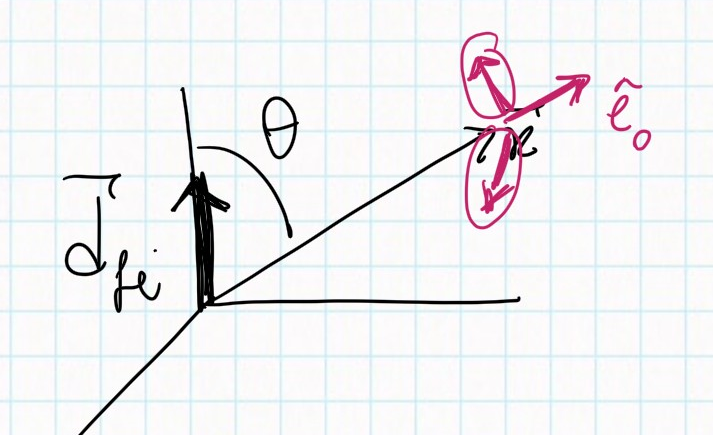
\includegraphics[scale=0.2]{Immagini/0310_sistema.png}
    \caption{Rappresentazione del sistema in esame.}
    \label{0310_sist}
\end{figure}
\newline
\noindent Soffermiamoci sull'elemento di matrice $|\hat{e}^*_{k\lambda}\cdot \vec{\mathrm{d}}_{fi}|^2$; poiché $\hat{e}_{kz'} = \hat{k}$ dovremo sommare\footnote{Con gli indici primati ci riferiamo al sistema di coordinate costruito sul versore di polarizzazione come in Figura \ref{0310_sist}.} solo su $\lambda = x',y'$:
$$\sum_{\lambda = x',y'}|\hat{e}^*_{k\lambda}\cdot \vec{\mathrm{d}}_{fi}|^2 = \sum_{\lambda=x',y',z'} |\hat{e}^*_{k\lambda}\cdot \vec{\mathrm{d}}_{fi}|^2 - |\hat{e}^*_{kz'}\cdot \vec{\mathrm{d}}_{fi}|^2 = \mathrm{d}_{fi}^2 -\mathrm{d}_{fi}^2\cos^2{(\theta)} = \mathrm{d}_{fi}^2 \sin^2{(\theta)} $$
Allora avremo per il rate:
\begin{displaymath}
\begin{aligned}
d\lambda &= \frac{2\pi}{\hbar} \delta(E_i-E_f-E_\gamma) \,\frac{e^2}{2}E_\gamma \mathrm{d}_{fi}^2 \sin^2(\theta) \,  \frac{k^2dkd\hat{k}}{(2\pi)^3} \\
%
p_\gamma = \hbar k \;\; E_\gamma = p_\gamma c &\qquad\frac{p^2_\gamma dp_\gamma}{\hbar^3} \to \frac{E_\gamma^2 dE_\gamma}{(\hbar c)^3}\\
%
\frac{d\lambda}{d\hat{k}} &= \frac{2\pi}{\hbar} \delta(E_i-E_f-E_\gamma) \,\frac{e^2}{2}E_\gamma \mathrm{d}_{fi}^2 \sin^2(\theta) \, \frac{E_\gamma^2 dE_\gamma}{(2\pi\hbar c)^3} \\
%
\Rightarrow \; \frac{d\lambda}{d\hat{k}} &= \frac{2\pi}{\hbar} \,\frac{e^2}{2}E_\gamma^3 \, \frac{\mathrm{d}_{fi}^2 \sin^2(\theta)}{(2\pi \hbar c)^3} \\
%
\frac{d\lambda}{d\hat{k}} &= \frac{1}{\hbar} \frac{\alpha}{2\pi}\,E_\gamma^3 \, \frac{\mathrm{d}_{fi}^2 \sin^2(\theta)}{( \hbar c)^2}
\end{aligned}
\end{displaymath}
dove nel penultimo passaggio abbiamo integrato la $\delta$ per cui $E_\gamma = E_i - E_f$ e nell'ultimo abbiamo sostituito la costante di struttura fine\index{costante di struttura fine@$\alpha$-costante di struttura fine} $\alpha$. Possiamo notare che abbiamo ottenuto un andamento del tipo $E^3_\gamma \sin^2(\theta)$ come nel caso classico.

\subsubsection{Riassunto}
Riassumiamo i concetti base del decadimento $\gamma$ che abbiamo visto nei paragrafi precedenti.
\begin{itemize}
    \item La parità dei termini di multipolo è opposta a parità di $J$.
    \item A parità di $J$ il contributo elettrico è maggiore rispetto a quello magnetico.
\end{itemize}

\paragraph{Regole di selezione} Poiché $\vec{J}_i = \vec{J}_f + \vec{J}$ ho che $\pi_i = \pi_f \cdot \pi(T_J)$, per cui non tutti i multipoli sono ammessi; infatti $|J_i - J_f|\leq J\leq J_i+J_f$:
\begin{itemize}
    \item Se $\pi_i = \pi_f$: allora per $M$ ho $J$ dispari e per $E$ ho $J$ pari.
    \item Se $\pi_i \not = \pi_f$: allora per $E$ ho $J$ dispari e per $M$ ho $J$ pari.
\end{itemize}
Notiamo che $J > 0$ anche se $J_i=J_f$, infatti se così non fosse (ovvero $J=0$) allora avremmo un fotone emesso lungo $\hat{k}$, ma questo non è possibile perché può avere solo polarizzazione $\pm 1$. Dunque le transizioni $0\to 0$ non sono ammesse\footnote{Queste si vedono, ma sono dovute a un processo differente, ovvero avvengono per \textbf{conversione interna}: il nucleo interagisce con un elettrone dell'atomo e quest'ultimo viene emesso.}.

\subsubsection{Alcuni esempi}
\paragraph{Primo esempio}
$$\ce{^{60}Co}  \xrightarrow{\beta^-} \ce{^{60}Ni}^*  \xrightarrow{\gamma}  \ce{^{60}Ni}$$

\begin{figure}[h]
    \centering
    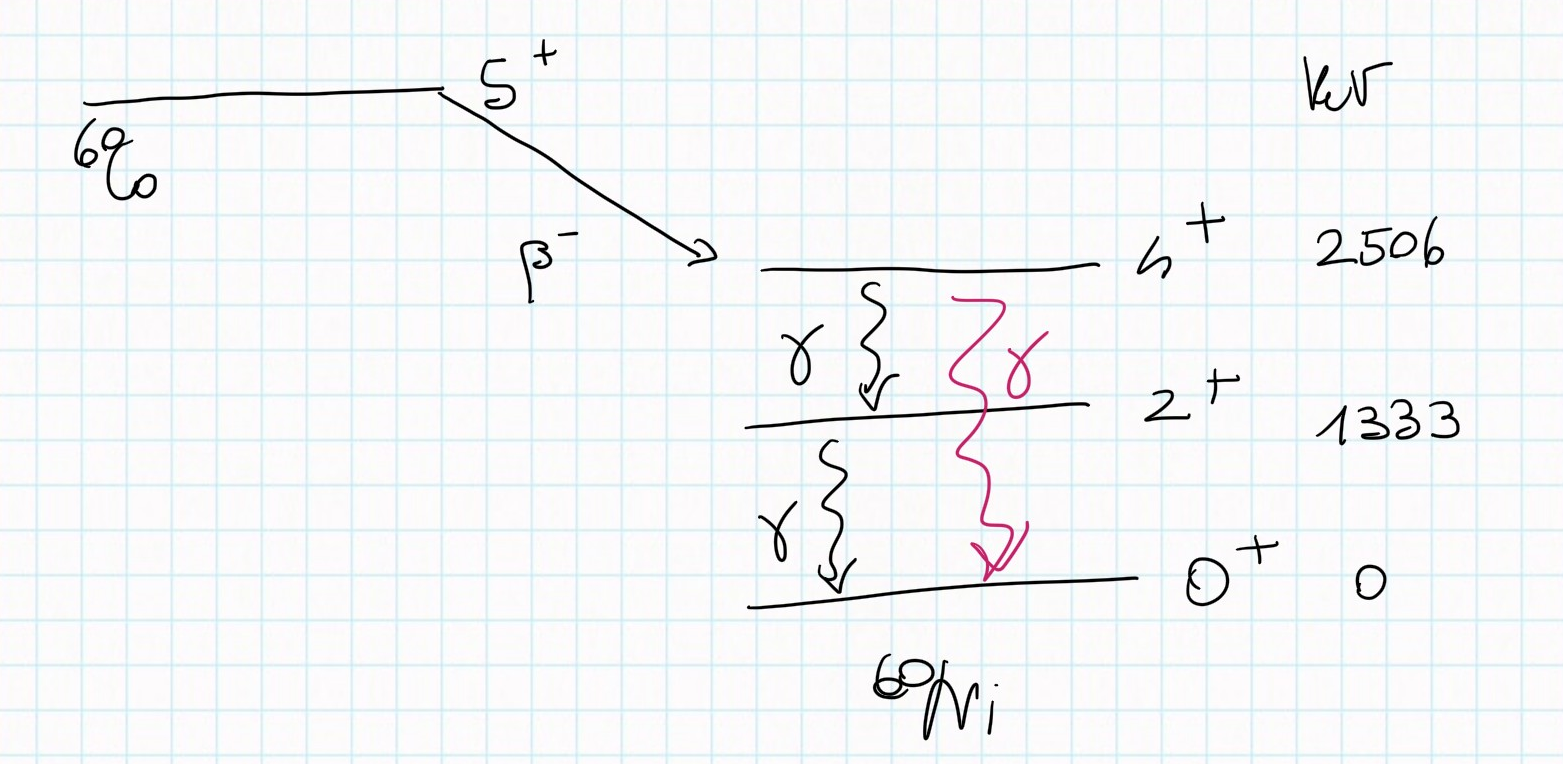
\includegraphics[scale=0.2]{Immagini/0310_bande.png}
    \caption{Schema delle bande rotazionali\index{bande rotazionali} coinvolte nel decadimento.}
    \label{0310_bande}
\end{figure}

\noindent Come mostrato nello schema in Figura \ref{0310_bande}, abbiamo 3 possibilità di decadimento:
\begin{itemize}
    \item $4^+\to2^+$: in questo caso $2\leq J\leq 6$ e $\delta \pi = 0$, allora avremo $E2,\,M3,\,E4,\,M5,\,E6$, dove domina per $E_\gamma\simeq 1.2$ MeV ($k\ll 1$) solo $E2$, con $M3$ come correzione.
    \item $2^+\to0^+$: in questo caso $J=2$ e $\delta \pi = 0$, allora avremo $E2$.
    \item $4^+\to0^+$: in questo caso $J=4$ e $\delta \pi = 0$, allora avremo $E4$.
\end{itemize}
\noindent  Per quanto riguarda le stime di Weisskopf\index{stime di Weisskopf}, ovviamente non saranno precise perché queste sono bande rotazionali\index{bande rotazionali}, quindi non è possibile fare l'approssimazione di simmetria sferica; tuttavia ci danno l'ordine di grandezza:
\begin{displaymath}
\begin{aligned}
\lambda(E2) &\simeq 7\cdot 10^7 \, 60^{4/3}\, (1.2)^5 \sim 2\cdot 10^{10} \unit{s}^{-1} & \tau_{dec} &= \frac{1}{\lambda} \sim 10^{-10} \unit{s} & 4^+&\to2^+ \\
%
\lambda(E2) &\simeq 7\cdot 10^7 \, 60^{4/3}\, (1.3)^5 \sim 2\cdot 10^{10} \unit{s}^{-1} & \tau_{dec} &= \frac{1}{\lambda} \sim 10^{-10} \unit{s} & 2^+&\to0^+ \\
%
\lambda(E4) &\simeq 10^{-5} \, 60^{8/3}\, (2.5)^5 \sim 2 \unit{s}^{-1} & \tau_{dec} &= \frac{1}{\lambda} \sim 0.5 \unit{s} & 4^+&\to0^+ 
\end{aligned}
\end{displaymath}
dove si può notare che tra $E2$ ed $E4$ c'è un fattore $10^{10}$. 

\paragraph{Secondo esempio}
$$\ce{^{137}Cs}  \xrightarrow{\beta^-} \ce{^{137}Ba}^*  \xrightarrow{\gamma}  \ce{^{137}Ba}$$

\begin{figure}[h]
    \centering
    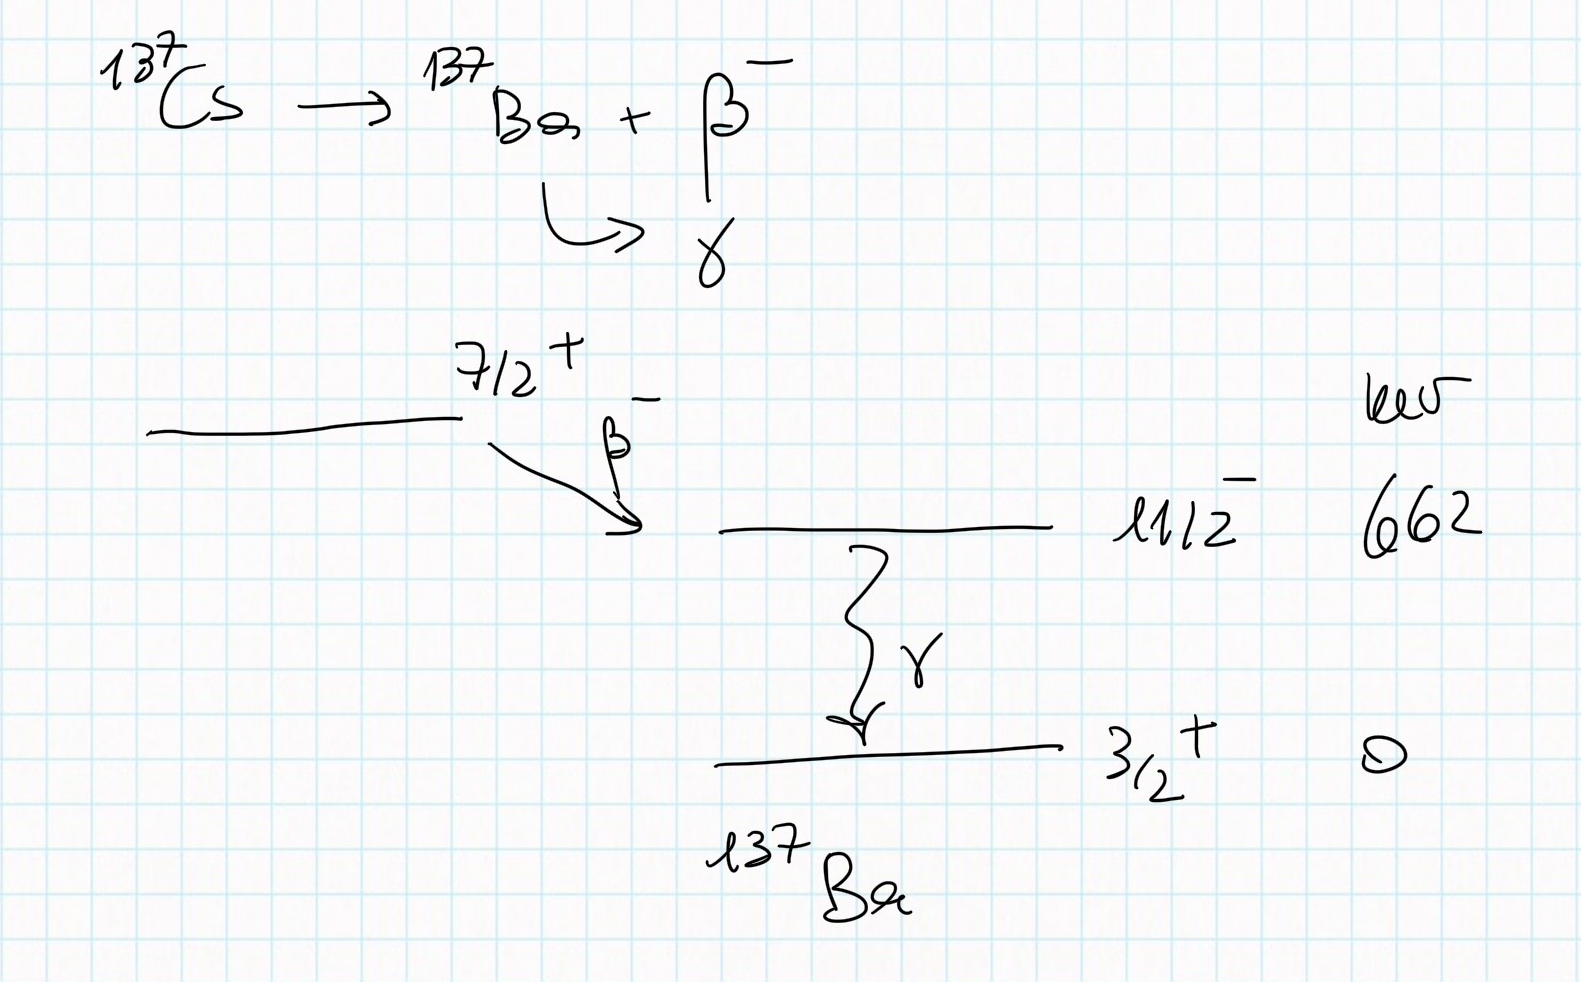
\includegraphics[scale=0.2]{Immagini/0310_bande2.png}
    \caption{Schema delle bande rotazionali\index{bande rotazionali} coinvolte nel decadimento.}
    \label{0310_bande1}
\end{figure}

\noindent In questo caso abbiamo la transizione $\frac{11}{2}^-\to\frac{3}{2}^+$ per cui $4\leq J \leq 7$ e $\Delta\pi \not = 0$; allora i termini di multipolo saranno $M4,\,E5,\,M6,\,E7$, dove $M4$ sarà dominante e $E5$ una piccola correzione.


\paragraph{Terzo esempio}
$$\ce{^{176}_{71}Lu}  \xrightarrow{\beta^-} \ce{^{176}_{72}Hf}^*  \xrightarrow{\gamma}  \ce{^{176}_{72}Hf}$$

\begin{figure}[h]
    \centering
    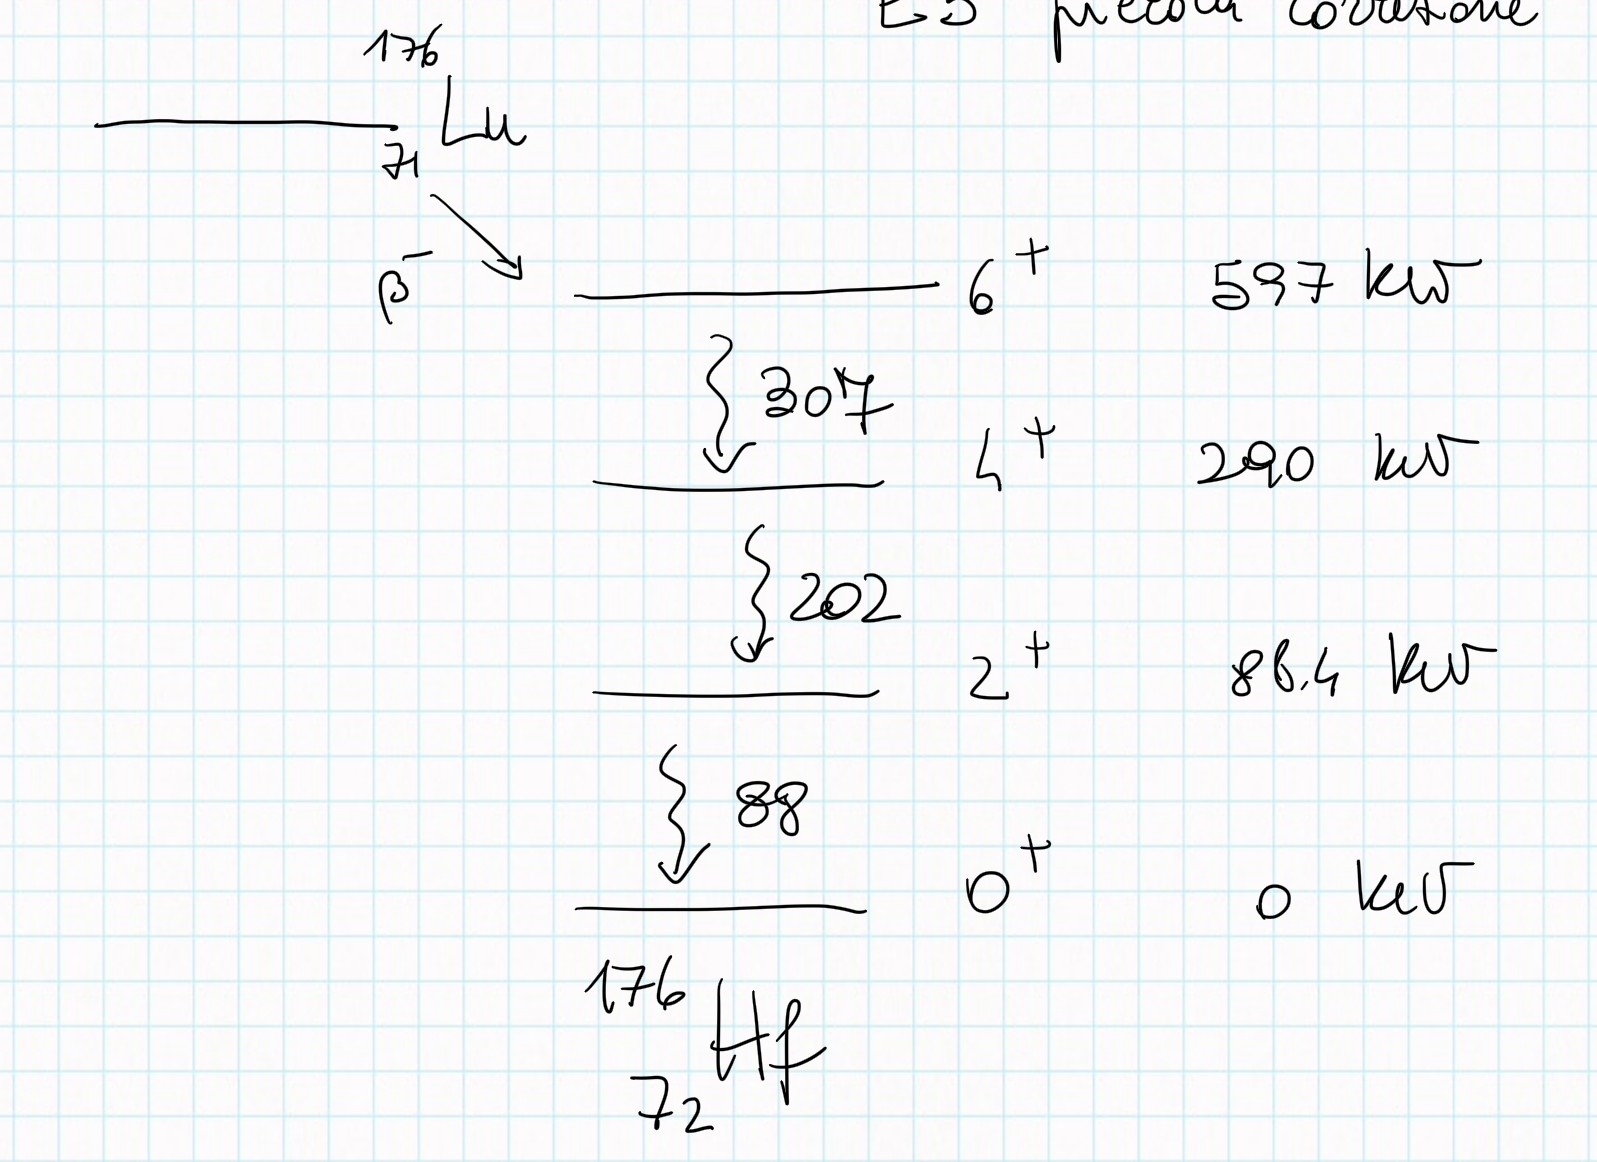
\includegraphics[scale=0.2]{Immagini/0310_bande3.png}
    \caption{Schema delle bande rotazionali\index{bande rotazionali} coinvolte nel decadimento.}
    \label{0310_bande2}
\end{figure}

\noindent In tutti i casi $\Delta\pi =0 $, studiamo $J$:
\begin{enumerate}[1.]
    \item $6^+\to4^+$: abbiamo $2\leq J \leq 10$, dominante $E2$.
    \item $4^+\to2^+$: abbiamo $2\leq J \leq 6$, dominante $E2$.
    \item $2^+\to0^+$: abbiamo $J=2$, dominante $E2$.
\end{enumerate}
Guardiamo le stime di Weisskopf\index{stime di Weisskopf}:
\begin{displaymath}
\begin{aligned}
1& & E2&\simeq 1.9 \cdot 10^8 \unit{s}^{-1} & \tau_{\frac{1}{2}} \simeq 3.6 \cdot 10^{-9} \unit{s} \\
2& & E2&\simeq 2.4 \cdot 10^7 \unit{s}^{-1} & \tau_{\frac{1}{2}} \simeq 2.9 \cdot 10^{-8} \unit{s} \\
3& & E2&\simeq 3.8 \cdot 10^5 \unit{s}^{-1} & \tau_{\frac{1}{2}} \simeq 1.8 \cdot 10^{-6} \unit{s} 
\end{aligned}
\end{displaymath}
Poiché i decadimenti 1 e 2 sono molto più veloci del decadimento 3 li osserverò come fondo di quest'ultimo (in un esperimento che ha come interesse lo studio del decadimento 3). Tuttavia, il risultato sperimentale del decadimento 3 $\tau_{\frac{1}{2}}^{oss}\simeq 1.43\cdot10^{-9}$ s non è assolutamente compatibile con quanto atteso; ciò è dovuto principalmente al fatto della asimmetria del nucleo, come già avevamo accennato: le stime di Weisskopf\index{stime di Weisskopf} non sono precise per nuclei particolarmente deformati (come in questo caso).

\subsubsection{Stato di scattering}
Vogliamo in questa trattazione studiare $J$, quindi non ci interessa che le particelle coinvolte siano nuclei o meno. Prendiamo lo stato di scattering:
$$n+p \to d + \gamma$$
Possiamo sempre definire lo stato iniziale come un autostato del momento $J$ ed espanderlo in onde parziali $\psi_{np}$. Allora avremo $\ell = 0,1,2,\dots$, ma dal momento che lo stato è di scattering (basse energie) ci interessa solo $\ell=0$; per quanto riguarda lo spin avremo $S=0,1$, tuttavia poiché i coefficienti di Clebsch-Gordan\index{coefficienti di Clebsch-Gordan} della transizione ${^3S_1}\to {^3S_1}$ sono trascurabili rispetto a quelli della transizione ${^1S_0}\to {^3S_1}$ avremo che rimarrà\footnote{Il pezzo di corrente di magnetizzazione in questo caso è rilevante.} solo $S=0$.\\
Dunque, abbiamo ${^1S_0}\to {^3S_1}$ con $J=1$ e $\Delta\pi  = 0$ e il termine dominante sarà $M1$.
    %   10/03
%%  Introduzione alla BBN
\newcommand{\sol}{_{\odot}}
\newcommand{\Msol}{$M\sol { }$}


%\part*{Lezione 11/03/2021}
\chapter{La Big Bang Nucleosynthesis}\label{cap-BBN}

\paragraph{Astronomical Observations}
Riportiamo adesso alcune informazioni generali su osservazioni astronomiche che ci serviranno per poterci poi concentrare sulla nucleosintesi primordiale e sulle reazioni all'interno delle stelle.



\begin{itemize}
    \item La Via Lattea\index{Via Lattea} è una galassia a spirale larga circa 30 kpc\footnote{Le misure sono riportate in \textit{parsec}\index{parsec}; ricordiamo che:
    $$1 \unit{pc} = 3\cdot 10^{16} \unit{m} = 3.3 \unit{ly}$$%
    } e spessa 1 kpc. \`E composta da $2\cdot 10^{11}$ stelle, polveri e gas. Il Sole è situato a circa 8.5 kpc dal centro galattico, che consiste in un buco nero supermassiccio\footnote{Se non fosse per il mezzo interstellare avrebbe una luminosità apparente pari a quella del Sole.} chiamato Sgr A$^*$\index{Sgr A$^*$}. La nostra Galassia insieme alla galassia di Andromeda\index{galassia di Andromeda} e una ventina di altre galassie nane forma il Gruppo Locale\index{Gruppo Locale}; questo è legato (gravitazionalmente) a sua volta ad altri gruppi con cui forma l'Ammasso della Vergine\index{Ammasso della Vergine} per un totale di circa $10^{10}$ galassie che occupano circa il $5\%$ dell'Universo.\\
    Le masse in gioco sono:
    $$M\sol\sim 2\cdot10^{30} \unit{kg}, \;\; \rho\sol \sim \rho_{\ce{H_2O}} \qquad M_{MW} > 2\cdot 10^{11} M\sol$$
    come abbiamo detto, non sono presenti solo stelle nella Via Lattea, ma anche mezzo e materia oscura. Per quanto riguarda il gas\index{gas@gas del mezzo interstellare}, questo ha una densità che varia da $10^9$ atomi/m$^3$ vicino al sistema solare fino a circa $10^5$ altrove e contiene principalmente H ed He con tracce di molecole.
    \item L'analisi spettrale\index{analisi spettrale} mi dà informazioni sulla temperatura e la composizione chimica.
    \item La luminosità\index{luminosità} è la densità di flusso di energia: $L = 4\pi R^2 \sigma\, T_{sup}^4$ dove $\sigma \equiv 5.7\cdot10^{-8}$ Wm$^{-2}$K$^{-4}$ è  la costante di Stefan-Boltzmann\index{costante di Stefan-Boltzmann@costante di Stefan-Boltzmann $\sigma$}; per cui:
    $$\Bigl ( \frac{L}{L\sol} \Bigr ) = \Bigl ( \frac{R}{R\sol}\Bigr )^2 \; \Bigl (\frac{T}{T\sol} \Bigr )^4$$
    Da questa relazione è possibile costruire un diagramma temperatura-luminosità detto diagramma Hertzsprung-Russell\index{diagramma Hertzsprung-Russell} in Figura \ref{0311_herz}. In questo grafico si osserva che le stelle in \textit{main sequence}\index{main sequence@\textit{main sequence}} si collocano quasi su una retta. Le rette grige corrispondono a linee lungo le quali si ha un raggio costante.
    \begin{figure}[h]
    \centering
    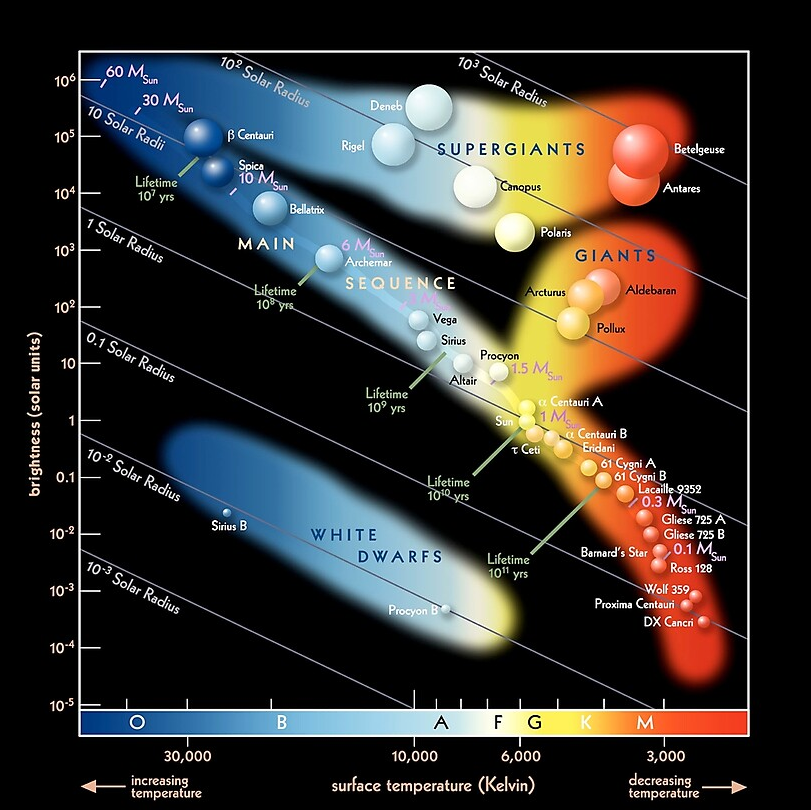
\includegraphics[scale=0.4]{Immagini/0311_herzprung1.png}
    \caption{Diagramma di Hertzsprung-Russell}
    \label{0311_herz}
    \end{figure}
    \item Nel 1930 Hubble si rende conto che le galassie sono uniformemente distribuite nel cielo\footnote{Da questo nascerà il Principio Cosmologico\index{Principio Cosmologico} per cui l'Universo viene assunto uniforme e isotropo (su \vir{grandi} scale).} e che si stanno allontanando. Tale deriva è osservabile dall'effetto Doppler\index{effetto Doppler} sulle righe spettrali di queste galassie, ovvero uno spostamento verso \vir{il rosso} (lunghezze d'onda maggiori); si definisce allora il parametro di \textit{redshift}\index{parametro di redshift@parametro di \textit{redshift} $z$}:
    $$z\equiv \frac{\lambda(v) - \lambda(0)}{\lambda(0)}\simeq \frac{v}{c}$$
    con $v\ll c$. Dalle osservazioni si evince che $z$ è proporzionale alla distanza $d$ dell'oggetto; la costante di proporzionalità tra la velocità di allontanamento e la distanza è detta costante di Hubble $H$\index{costante di Hubble@costante di Hubble $H$}. Sul valore di questa costante c'è tensione, riportiamo il valore ottenuto dalla misura sulle scale di distanza: $H= 72\unit{km}\,\mbox{s}^{-1}\mbox{Mpc}^{-1} \simeq 2.3\cdot 10^{-18}\unit{s}^{-1}$. Ipotizzando che il rate di espansione sia rimasto sempre lo stesso allora $H^{-1}$ dà una stima dell'età dell'universo $t\sim 12 \cdot 10^9\unit{y}$.
    \item Nasce così l'idea (riavvolgendo nel tempo l'espansione) di un punto di inizio da cui tutto è partito: il \textit{Big Bang}\index{Big Bang@\textit{Big Bang}}. Secondo questa teoria, materia e radiazione erano inizialmente accoppiate fino a un tempo di disaccoppiamento e di successiva ricombinazione tra i barioni. Da quel momento in poi la radiazione (su larga scala) non ha più interagito con la materia e infatti si osserva un fondo di radiazione cosmica detto \textit{Cosmic Microwave Background}\index{Cosmic Microwave Background@Cosmic Microwave Background CMB} (CMB), ancora oggi molto studiato. La teoria prevedeva\footnote{Questi valori dipendono fortemente dal modello.} una $\lambda\simeq 7.5\unit{cm}$ (da cui il nome \textit{microwave}), che per un corpo nero corrisponde a $T\simeq 2.7\unit{K}$, e fu osservato nel 1965 da Penzias e Wilson. 
    \item Per misurare $H_0$ (dove il pedice indica che la costante è misurata per il tempo attuale) si utilizzano principalmente 2 metodi: l'osservazione dell'espansione dell'Universo dagli spettri delle galassie lontane oppure delle disomogeneità nel CMB.
    Nel primo caso, è necessario selezionare galassie per cui la velocità di espansione è più rilevante rispetto alla velocità peculiare\index{velocità peculiare}\footnote{Si tratta della velocità di avvicinamento dovuta alle interazioni gravitazionali tra galassie ed è dell'ordine del 100 km/s.} e misurarne le distanze; a tal scopo si fa uso di candele campione\index{candela campione} (oggetti con poca astrofisica, ben identificabili) e dalla legge di Hubble\index{legge di Hubble} ottengo una stima indipendente dal modello cosmologico di $H_0$.\\ 
    Nel metodo della CMB, invece, si osservano le sovradensità dovute a fluttuazioni in densità dell'ordine di $10^{-2}$ nell'Universo primordiale che hanno portato a un gradiente di pressione, quindi a onde sonore; al momento della ricombinazione queste oscillazioni si sono congelate e ci aspettiamo quindi dei picchi in queste fluttuazioni detti appunto \textit{acoustic peaks}\index{acoustic peaks@\textit{acoustic peaks}}, visibili per alcuni $\Vec{k}$ tramite un'analisi spettrale, come mostrato in Figura \ref{0311_peak}. Questi picchi dipendono da alcuni parametri cosmologici tra cui $\Omega_b$ che è legata alla densità critica $\rho_c\equiv 3H_0^2/8\pi G$\index{densità critica@densità critica $\rho_c$}, per cui si ottiene una stima di $H_0$, ma che dipende fortemente dal modello. Come si vede in Figura \ref{0311_H0} vi è tensione e ancora oggi si sta cercando una risposta.
    \begin{figure}[h]
        \centering
        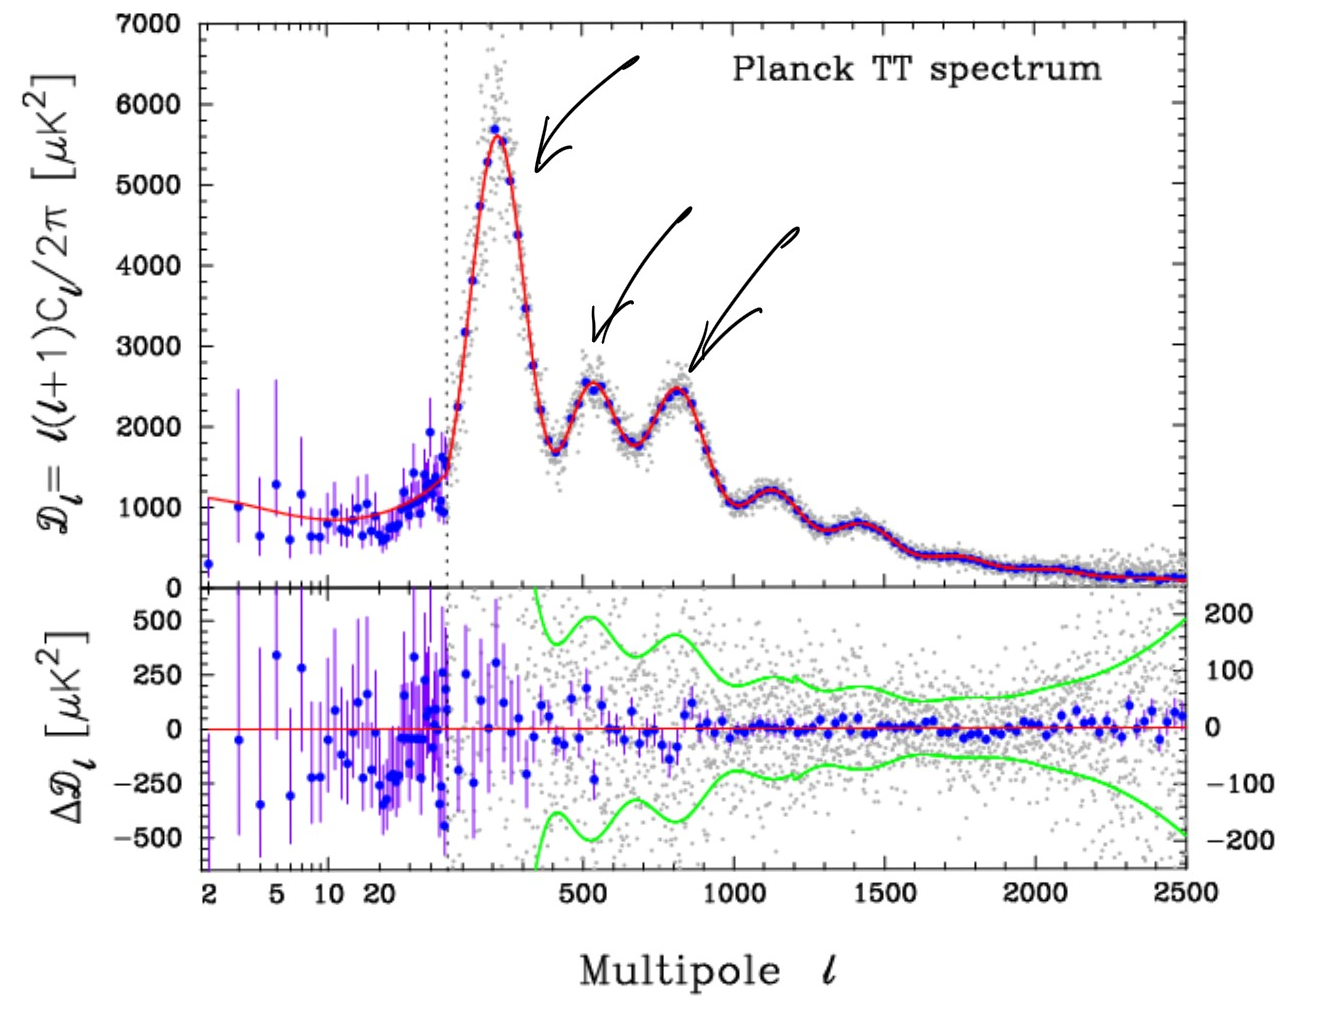
\includegraphics[scale=0.2]{Immagini/0311_peak.png}
        \caption{Analisi spettrale della sovradensità nel CMB. Si possono osservare i picchi di cui parlavamo.}
        \label{0311_peak}
    \end{figure}
    \begin{figure}[h]
        \centering
        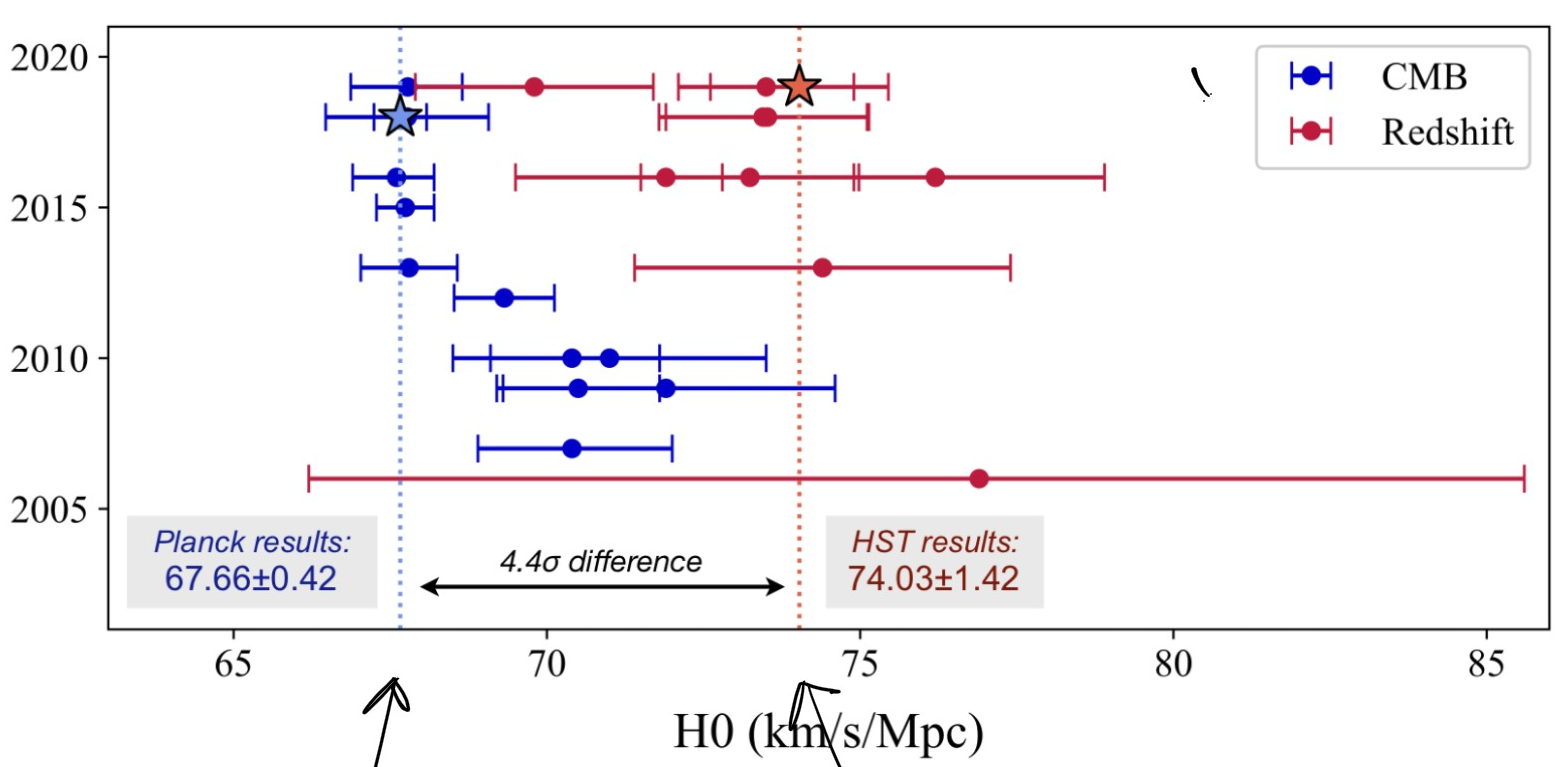
\includegraphics[scale=0.2]{Immagini/0311_peak2.png}
        \caption{Tensione per le misure di $H_0$. Si osserva che nel tempo i valori si sono allontanati.}
        \label{0311_H0}
    \end{figure}
\end{itemize}
\noindent Queste osservazioni ci hanno portati alla teoria del \textit{Big Bang}, necessaria per introdurre il prossimo fondamentale argomento, ovvero la trattazione dei meccanismi e delle tipologie delle reazioni nucleari che hanno caratterizzato l'Universo primordiale, detta \textit{\textbf{Big Bang Nucleosynthesis Theory}}\index{Big Bang Nucleosynthesis} (\textbf{BBN}).


\section{Introduzione alla teoria}
Il \textit{Big Bang model} comporta necessariamente la formulazione di una teoria sulla nucleosintesi primordiale. Questa fu trattata per la prima volta in un articolo del 1940 degli autori Gamow, Adler e Bethe\index{articolo Adler, Bethe, Gamow@articolo $alpha,\,\beta,\,\gamma$}\footnote{Un aneddoto diverte: Gamow (che è lo stesso Gamow del decadimento di Gamow-Teller\index{decadimento!Gamow-Teller}) insistette per avere la partecipazione anche di Bethe, per poter mettere nell'articolo i nomi \vir{Adler, Bethe, Gamow} che ricordavano $\alpha,\,\beta,\,\gamma$, nome con cui ormai viene ricordato l'articolo.}.

\paragraph{Il problema di $Y_P$} Prima di passare allo studio delle reazioni di interesse, mostriamo come alcuni risultati confermano la necessità di una nucleosintesi primordiale.\\
Se assumiamo che $M_{MW} \sim 10^{11}$ \Msol e $L_{MW}\sim 2\cdot \ord{10}\unit{L}\sol {}$ allora l'energia totale liberata in un tempo $H_0^{-1}$ sarà $E_{tot} \simeq L_{MW}/H_0\sim 2.4\cdot 10^{54}\unit{J}$; escludendo la nucleosintesi primordiale l'unica reazione possibile è $4p\to\ce{^4He}$, allora $E_{\ce{^4He}} = 28\unit{MeV}= 4.5 \cdot \ord{-12}\unit{J}$. Se tutta la massa stellare bruciasse allora si libererebbe un'energia pari a $E_{burn} \equiv E_{\ce{^4He}}\cdot M_{MW}/4m_p\sim 1.3\cdot \ord{56}\unit{J}$, da cui otteniamo $E_{tot}/E_{burn}\sim 2\%$ che corrisponde alla percentuale in massa di $\ce{^4He}$ \vir{primordiale} $Y_P$. Tuttavia, sperimentalmente si osserva che $Y_P\simeq 25\%$, dunque le reazioni nucleari nei core stellari non sono sufficienti per spiegare questa abbondanza ed è necessario introdurre un altro meccanismo (la nucleosintesi primordiale, appunto).

\paragraph{A grandi linee}\label{a.grandi.linee} Proviamo a correggere il risultato precedente con argomentazioni qualitative. Ovviamente per la nostra trattazione non siamo interessati al \textit{Big Bang}\index{Big Bang@\textit{Big Bang}}, ma fisseremo come origine dei tempi l'attimo prima che protoni e neutroni si formino: 
\begin{itemize}
    \item a $t=0\unit{s}$ abbiamo quindi una sfera molto densa e molto calda $T>\ord{13}\unit{K}$.  
    \item a $t\sim 0.01\unit{s}$ domina ancora la radiazione e non riescono a formarsi protoni e neutroni perché $T\sim\ord{13}$ quindi $E=kT\sim 1\unit{GeV}$, quindi anche se ci fossero $p$ e $n$ verrebbero fotodisintegrati.
    \item a $t\sim 0.1\unit{s}$ la temperatura scende a $T\sim 3\cdot\ord{10}\unit{K}$ per cui $E\simeq 3\unit{MeV}$ e si formano finalmente protoni e neutroni.\\ 
    A questo punto è fondamentale ricordare che la massa del neutrone è maggiore di quella del protone $\Delta m = 1.3\unit{MeV}$ per cui avremo al momento del \textit{Freeze-out}\index{Freeze-out@\textit{Freeze-out}}:
    $$\frac{N_n}{N_p}\propto \exp{\ppc{-\frac{\Delta m}{kT}}} \simeq 0.22 \simeq \frac{1}{5}$$
    per cui per 1000 protoni abbiamo 220 neutroni circa. Ancora non si può formare il deutone.
    \item a $t\sim 180\unit{s}$ la temperatura raggiunge $T\sim \ord{9}\unit{K}$ a cui corrisponde $E\sim 0.09\unit{MeV}$ e quindi si possono formare i nuclei. Tuttavia, è necessario ricordare che il neutrone decade con una legge del tipo $N_n(t) = N_n^0 \, \exp{(-t/\tau_n)}$ con $\tau_n \sim 886\unit{s}$; nell'esempio da noi fatto ($N_n^0= 220$) avremo $N_n \simeq 180$ e $N_p = N_p^0 + (N_n^0-N_n) = 1040$.
\end{itemize}
\noindent Allora possiamo ipotizzare che qualitativamente\footnote{In realtà esiste un \textit{full network} di relazioni.} avremo queste relazioni:
\begin{displaymath}
\begin{aligned}
n + p &\to d + \gamma \\
n + d &\to \ce{^3H} + \gamma \\
\ce{^3H} + p &\to \ce{^4He} + \gamma
\end{aligned}
\end{displaymath}
Ci chiediamo quanto valga $Y_P$:
\begin{displaymath}
\begin{aligned}
Y_P &= \frac{4 N_{\ce{He}}}{N_{p,\text{rimasto} + 4N_{\ce{He}} }} \;\leftarrow\: \text{Mass fraction}\\
&= \frac{4 \frac{N_n}{2}}{(N_p - N_n) + 4\frac{N_n}{2}} = \\
&\simeq 0.29
\end{aligned}
\end{displaymath}
che si avvicina molto al 25\% cercato.




        %   11/03
%%  Network della BBN
%\part*{Lezione 15/03/2021}

\paragraph{Le basi della BBN} Innanzitutto elenchiamo gli \vir{ingredienti} essenziali della BBN:
\begin{itemize}
    \item Un network di reazioni.
    \item Il numero di neutroni e protoni di partenza, che sarà determinato, come abbiamo accennato, dalla vita media del neutrone, misura sulla quale tuttora è presente una certa incertezza (fornitaci dal PDG\footnote{PDG = Particle Data Group.}).
    \item Il rapporto tra barioni e fotoni detto \textbf{\textit{entropy factor}} $\eta$\index{entropy factor@\textit{entropy factor} $\eta$}\footnote{\acc{E} definito come rapporto tra la densità barionica e quella dei fotoni $n_b/n_\gamma$.}. Questo parametro ci dice se è favorita la ricombinazione ($\eta$ grande) o la fotodisintegrazione della materia.
    \item Il fattore $\eta$ è legato alla \textbf{\textit{barion density}}\index{barion density@\textit{barion density} $\rho_B$} secondo $\rho_B = 6.8\cdot\ord{-22}\unit{g cm}^{-3}\; \cdot \eta$. Spesso però al posto di questa si tende a lavorare con la \textbf{\textit{barion fraction of critical mass density}}\index{barion fraction of critical mass density@\textit{barion fraction of critical mass density} $\Omega_B h^2$}, definita come $\Omega_B h^2= 3.6 \cdot\ord{7}\;\cdot \eta$\footnote{Dove $h$ è un parametro adimensionale per la costante di Hubble, definito come $h=H_0/100 [\mbox{km}/\mbox{s Mpc}]$.}.
\end{itemize}
Come \vir{output} da questi avremo le abbondanze degli elementi primordiali (ovvero H, He e metalli leggeri). Passiamo allora alla trattazione di questi \vir{input}.

\section{Network di reazioni}
In Figura \ref{0315_net} riportiamo le reazioni coinvolte nella nucleosintesi primordiale; nel seguito con i numeri puntati tra parentesi (per esempio (1.), (2.)) faremo riferimento alle reazione riportate in questa figura.
\begin{figure}[h]
    \centering
    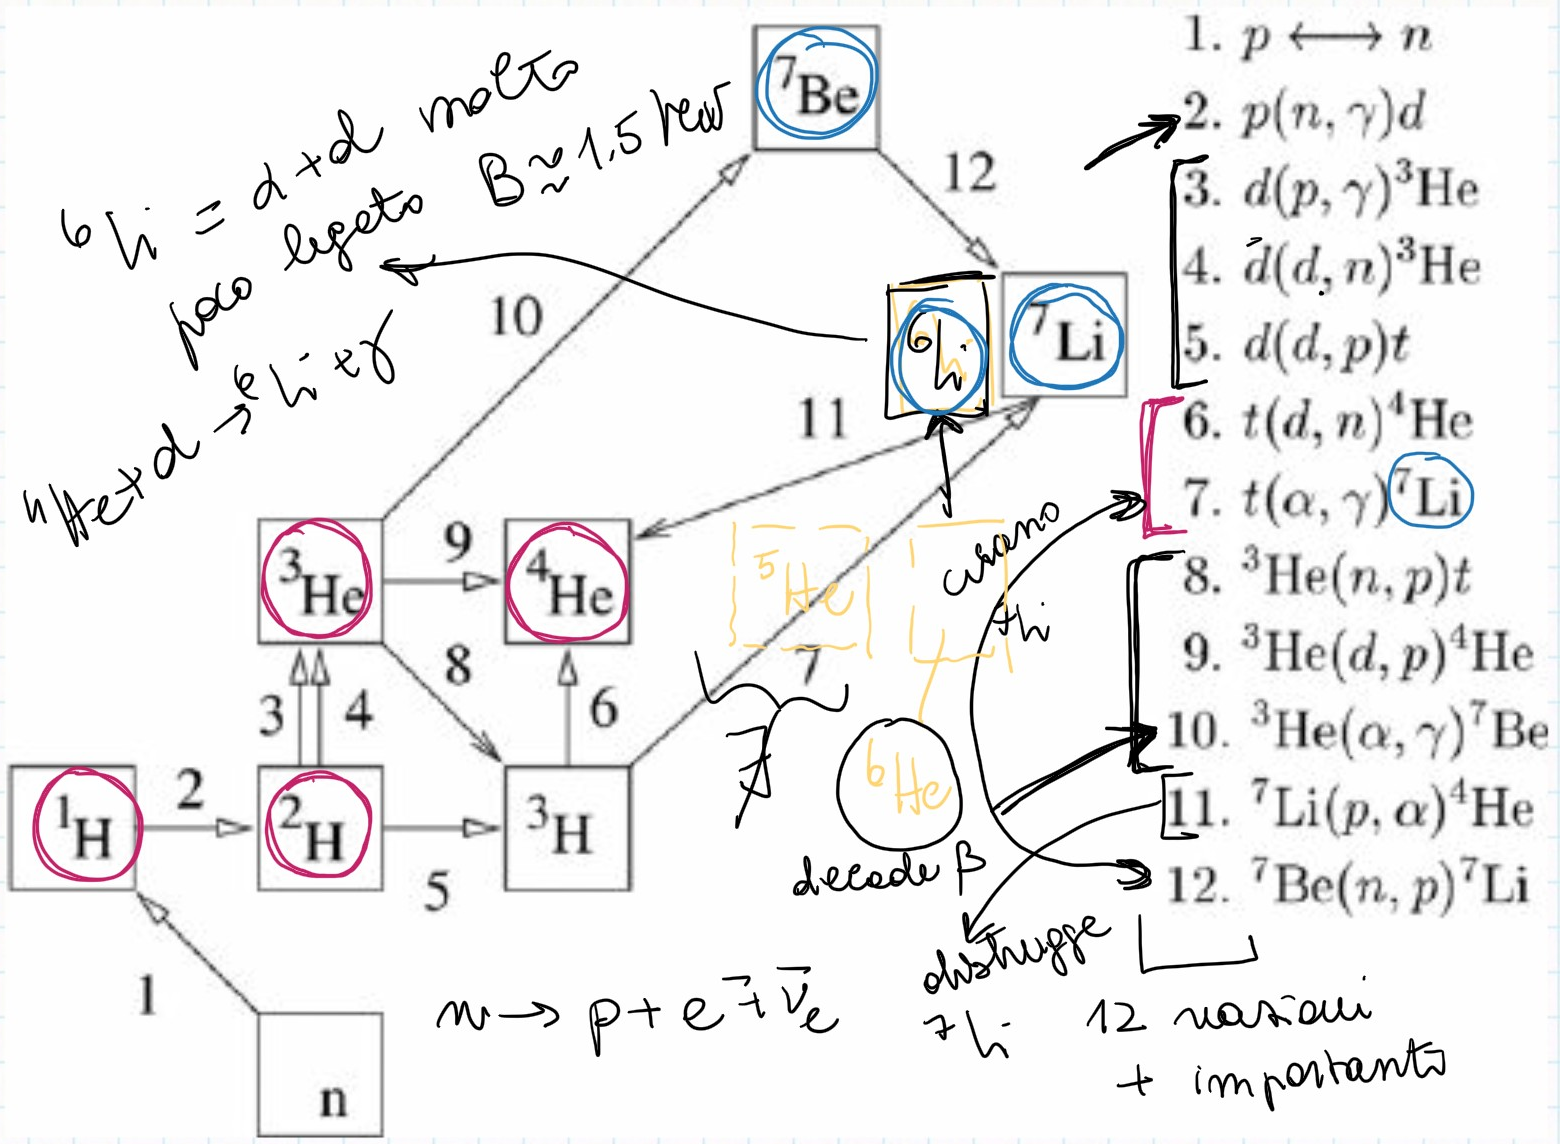
\includegraphics[scale=0.25]{Immagini/0315_network.png}
    \caption{Sono riportate le 12 reazioni più importanti. Gli elementi segnati in rosa sono i primordiali più abbondanti.}
    \label{0315_net}
\end{figure}

\paragraph{Criteri qualitativi di reazione} Prima di procedere ricordiamo alcune regole qualitative per capire quale tra i vari rami di una reazione è favorito rispetto agli altri:
\begin{itemize}
    \item[I] $\sigma_\text{forte}\gg\sigma_\text{EM}\gg\sigma_\text{debole}$. Per riconoscere a quale tipo di interazione appartiene la reazione è sufficiente osservare i prodotti: se compaiono neutrini l'interazione è debole, se invece il numero di protoni e neutroni è conservato abbiamo interazione forte e se si ha anche produzione di un fotone allora si ha interazione elettromagnetica.
    \item[II] L'abbondanza dei reagenti è discriminante.
    \item[III] La barriera Coulombiana da superare per avere la reazione è un fattore che influisce fortemente sulla probabilità di reazione.
\end{itemize}

\subsection{La nucleosintesi primordiale}\label{sec-nuc-prim}
La prima reazione che abbiamo è il decadimento del neutrone\footnote{Si tratta dell'unica reazione di interazione debole.} (1.); successivamente segue una cattura radiativa $p$-$n$ (2.) e a questo punto abbiamo 3 possibili reazioni di distruzione del deuterio: secondo il I criterio la (4.) e la (5.) dovrebbero contare maggiormente rispetto alla (3.), ma poiché l'abbondanza di $p$ è superiore a quella di $d$ le probabilità delle tre reazioni sono dello stesso ordine\footnote{Si capisce allora come mai non si ha $d(d,\gamma)\ce{^4He}$ (poca abbondanza e interazione EM).}. Queste reazioni non sono sufficienti a consumare tutto il deuterio, che potrà interagire con il trizio $t$ secondo la (6.); il trizio non è un elemento primordiale perché decade, ma essendo un decadimento debole è molto probabile che interagisca nuovamente con $\alpha$ (7.) dando $\ce{^7Li}$\footnote{Vedremo che la presenza di questo $\ce{^7Li}$ sarà una questione delicata da trattare.}.
Per quanto riguarda $\ce{^3He}$, invece, questo è stabile e ha varie reazioni di distruzione\footnote{Esisterebbe anche $\ce{^3He}(n,\gamma)\ce{^4He}$, ma la (8.) (data l'abbondanza e la natura dell'interazione) è molto più importante.}, tra cui la più importante se ancora vi sono neutroni è la (8.), alla quale segue (nonostante la poca abbondanza di deuterio) la (9.) e quando si raggiunge un certo numero di $\ce{^3He}$ e $\alpha$ si ha anche la (10.); ora il berillio che si è formato da questo viene distrutto praticamente tutto in $\ce{^7Li}$ (12.).\\
Fermiamoci un attimo: come mai non troviamo reazioni per $\ce{^5He}$, $\ce{^6He}$ e $\ce{^6Li}$? Allora il $\ce{^5He}$ non è uno stato legato, ma $\ce{^6He}$ sì, tuttavia questo decade $\beta$ molto velocemente (è poco legato) in $\ce{^6Li}$. Quest'ultimo si ottiene anche da $\alpha + d$ con l'emissione di un fotone e il motivo per cui la sua abbondanza non è significativa è dovuto al fatto che è poco legato, per cui si rompe facilmente.\\
Abbiamo ancora un problema da risolvere, ovvero che la carta dei nuclei presenta un \textit{gap} per $A=8$: il $\ce{^8B}$ e il $\ce{^8Li}$ decadono $\beta$ e il $\ce{^8Be}$ decade $\alpha$. Dunque, la BBN si ferma qui\footnote{In realtà esistono reazioni per saltare da $A=5$ ad $A=7$, ma sono comunque trascurabili rispetto a tutti gli altri processi.} con $p$, $\ce{^2H}$, $\ce{^3He}$, $\ce{^4He}$, $\ce{^7Li}$ (poco) e $\ce{^7Be}$ (pochissimo).

\paragraph{Confronto con le osservazioni} A questo punto per studiare la BBN è necessario prendere i valori delle varie sezioni d'urto delle reazioni coinvolte e vederne l'evoluzione temporale, come mostrato in Figura \ref{0315_mfrac}, dove è riportata la \textit{mass fraction} dei principali elementi predetta dal modello\footnote{Una piccola nota sul berillio: non è facile da misurare, quindi spesso quello che si misura è il rapporto $d/\ce{H}$ o $\ce{^3He/H}$.}. Dunque, dalle misure di queste quantità è possibile stimare la bontà della teoria.

\begin{figure}[h]
    \centering
    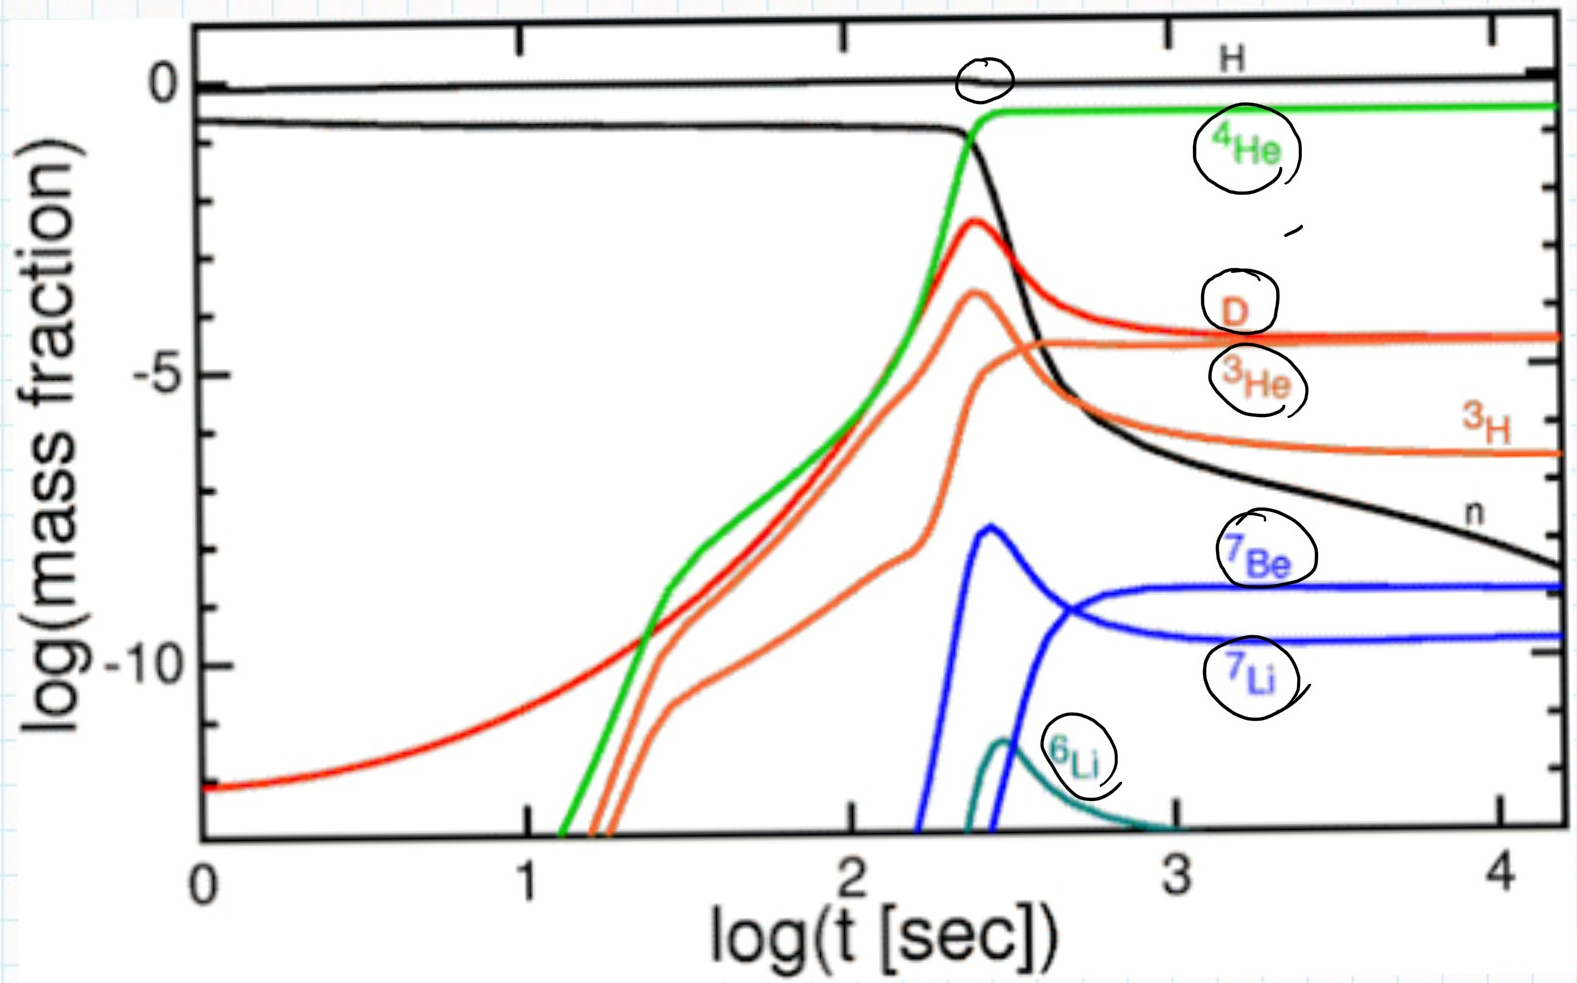
\includegraphics[scale=0.2]{Immagini/0315_massfraction.png}
    \caption{Andamento nel tempo della \textit{mass fraction}, ovvero dell'abbondanza di un elemento sull'abbondanza di $\ce{H}$. L'abbondanza di $\ce{H}$ ha un leggero scalino e quello segna l'inizio della BBN; si vede che $n$ decade; il $\ce{^3H}$ è indicato, ma decade; vi è un errore per l'andamento del $\ce{^6Li}$, dovrebbe essere più alto.}
    \label{0315_mfrac}
\end{figure}

\noindent Riportiamo allora le osservazioni in Figura \ref{0315_mfrac2}. Da queste misure è possibile stimare $\Omega_B h^2$ e alla fine degli anni '90 si ebbe la prima evidenza che la densità di materia dell'Universo fosse differente da quella attesa (a causa dell'assenza nel conto del contributo dovuto alla materia oscura). 

\begin{figure}[h]
    \centering
    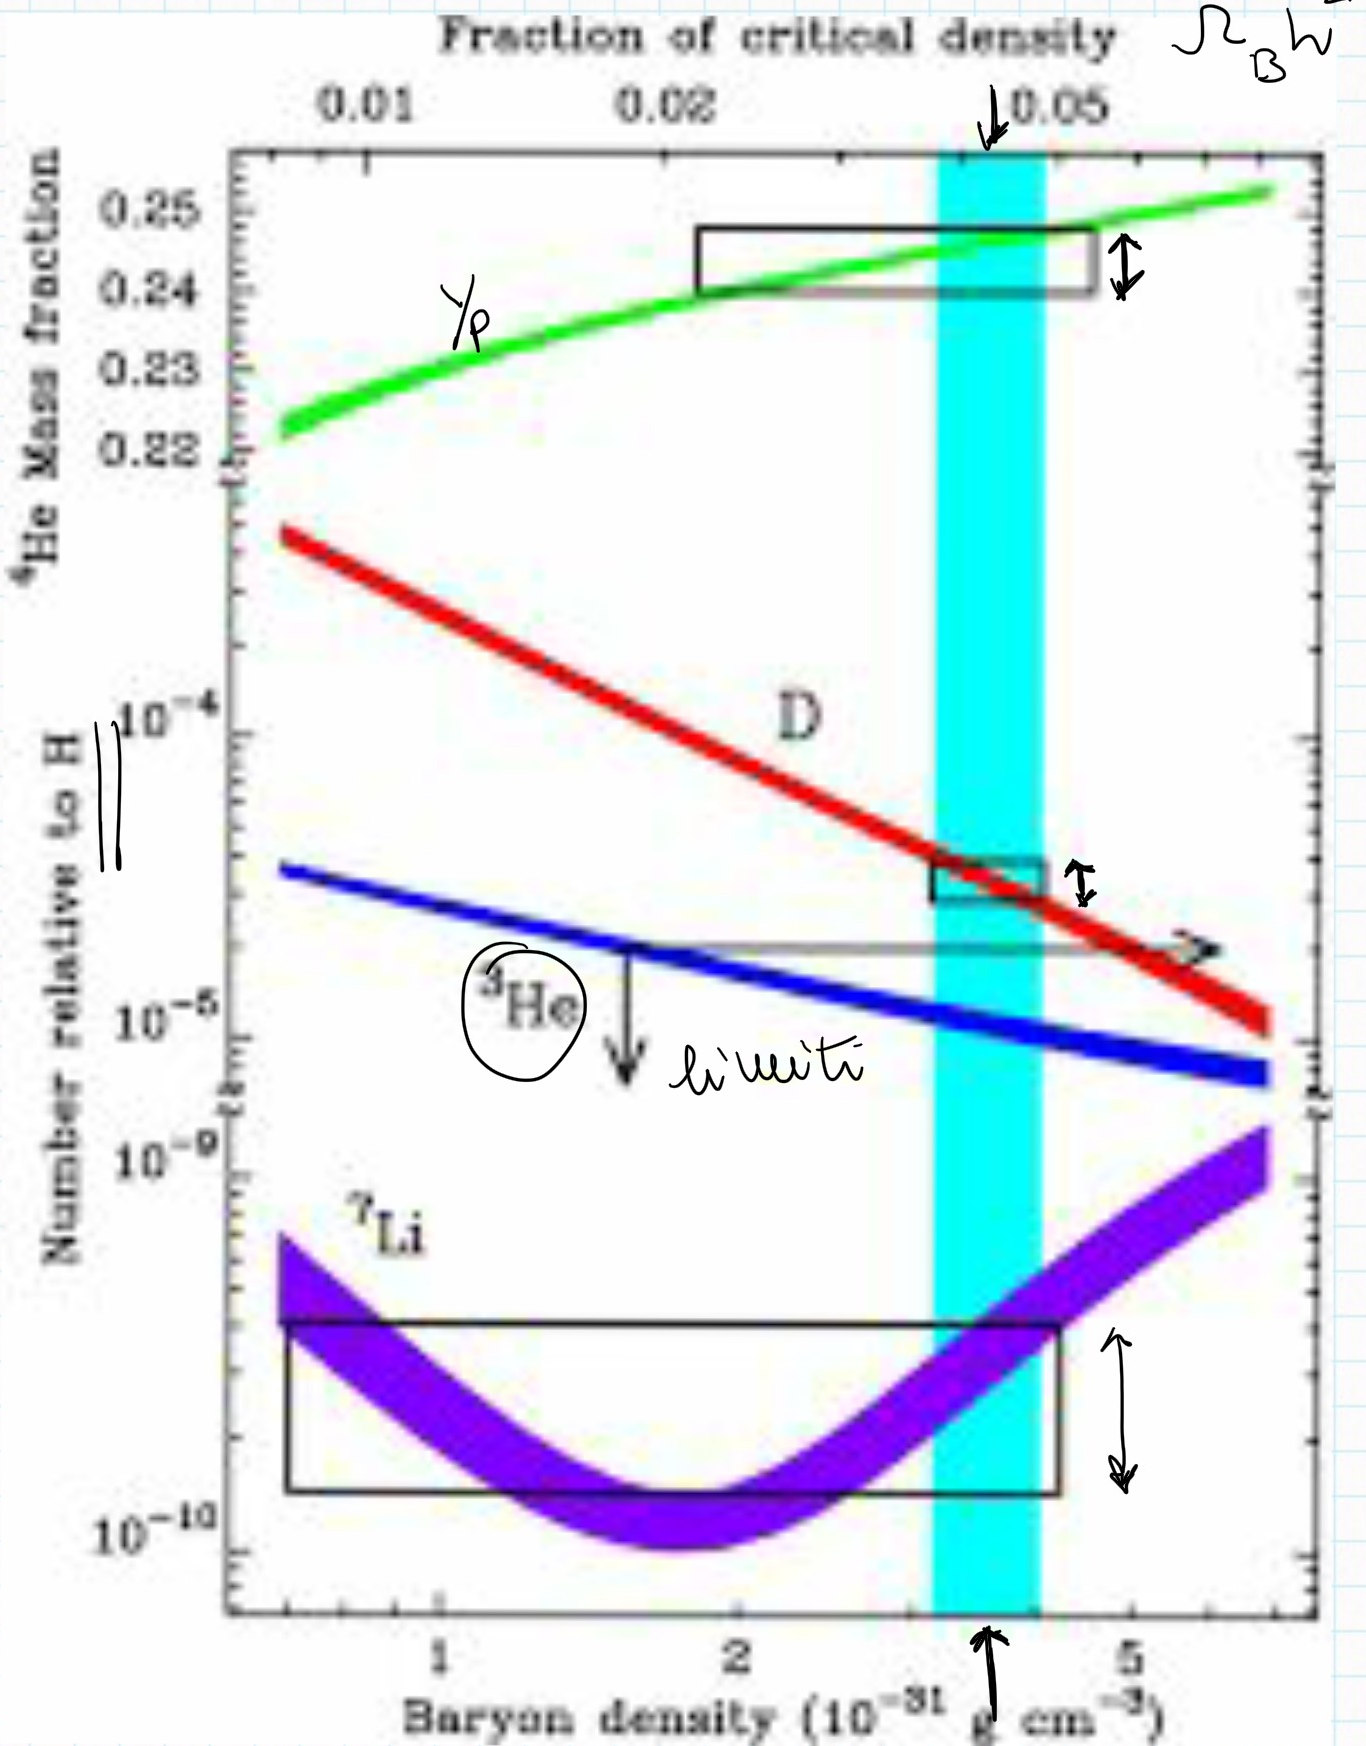
\includegraphics[scale=0.2]{Immagini/0315_massfraction2.png}
    \caption{Le bande degli andamenti sono dovute alle incertezze. Coi rettangoli si riportano le misure. Il range di interesse è indicato dalla striscia celeste. Per il trizio ci sono solo limiti superiori e inferiori.}
    \label{0315_mfrac2}
\end{figure}

\paragraph{Misurazione delle abbondanze primordiali} Partiamo dalla misura per $\ce{^4He}$. I primi problemi sorgono dal fatto che le stelle ne hanno aumentato la concentrazione, dunque si fanno misure del rapporto $\ce{^4He}/\ce{H}$ in regioni in cui è avvenuta poca o quasi nulla evoluzione stellare, ovvero galassie \textit{metal-poor}. Riportiamo in Figura \ref{0315_Hefrac} un esempio. A oggi si ha un valore di circa $Y_p \sim 0.25$.

\begin{figure}[!h]
    \centering
    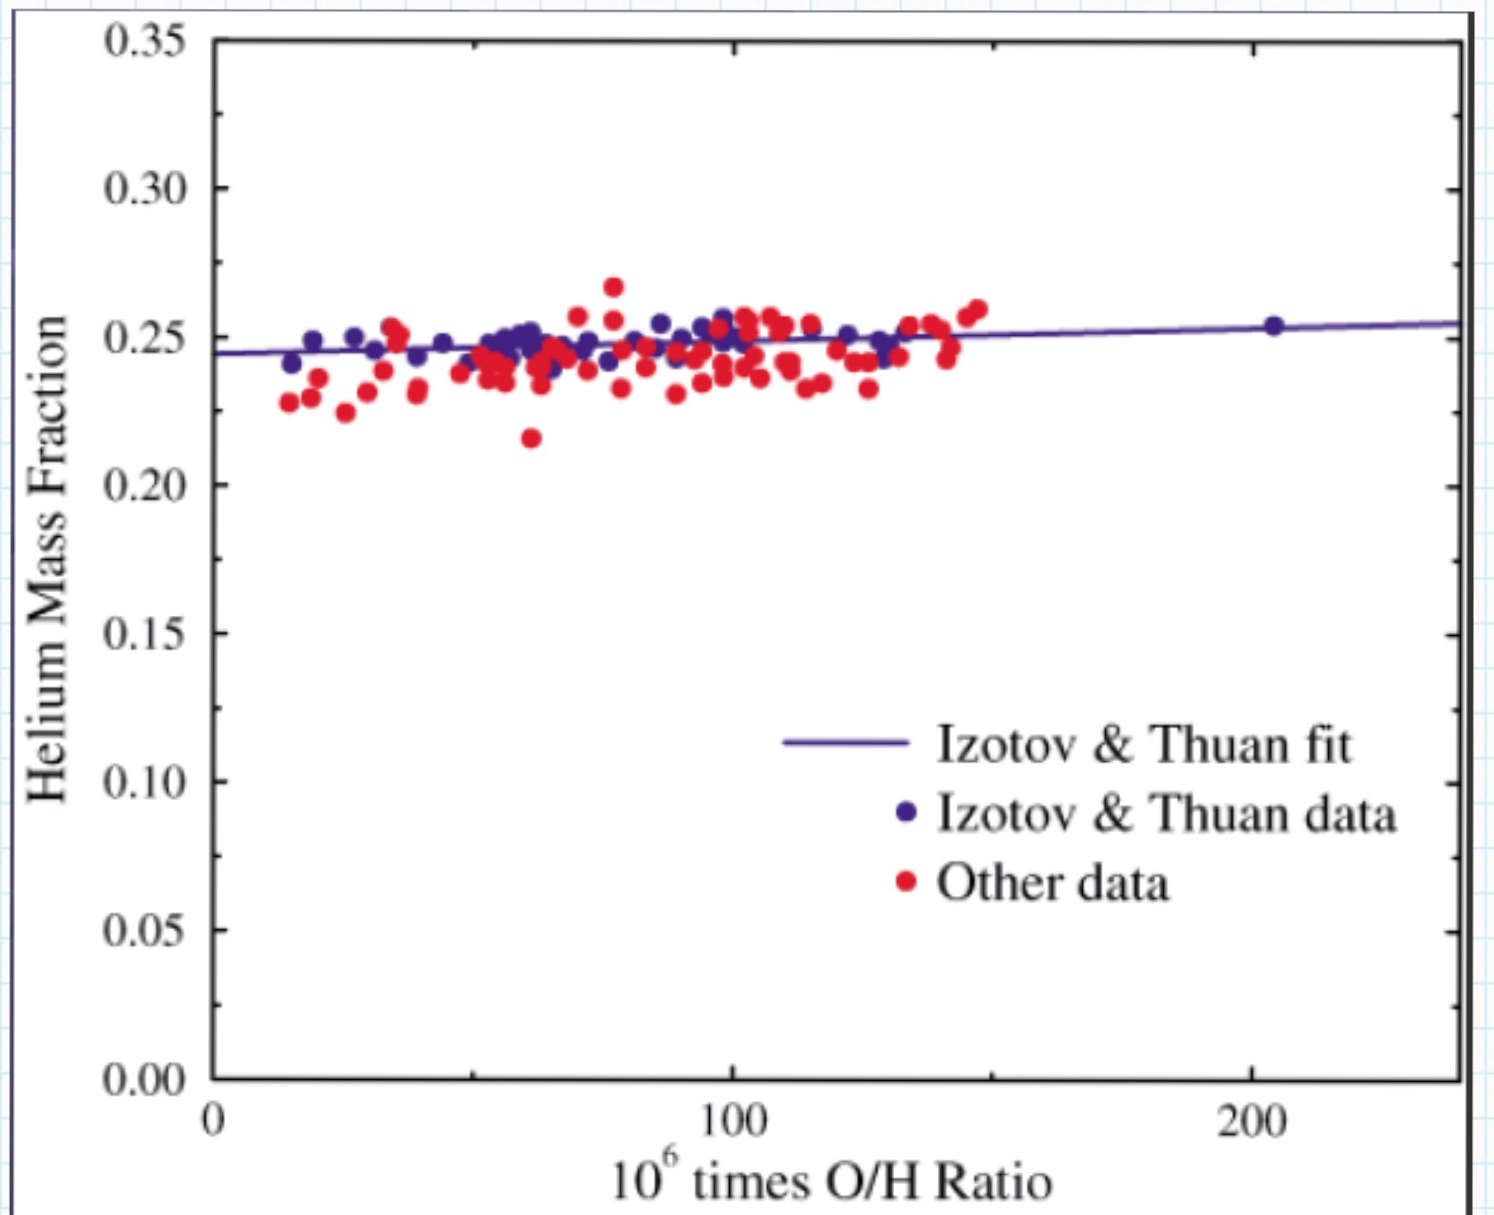
\includegraphics[scale=0.2]{Immagini/0315_heliummassfraction.png}
    \caption{Risultati sperimentali per stelle con metallicità differente.}
    \label{0315_Hefrac}
\end{figure}

\noindent La misura del deuterio è anche più problematica: esso infatti è \vir{fragile}, per cui vanno evitate le stelle e gli oggetti densi, anzi si fanno osservazioni nel mezzo interstellare.\\
Il 1973 il satellite Copernico riuscì a dare dei limiti (superiori e inferiori), ma non a raccogliere dei veri e propri dati. Successivamente, nel 1998, Tytler e Burles ebbero un'idea, ovvero quella di misurare $d/\ce{H}$ nelle \textit{hydrogen clouds} ad alto \textit{redshift}\index{redshift@\textit{redshift}} ($z>3$, oggetti molto vecchi): si osservano le linee di assorbimento della Ly$\alpha$\index{Lymann@Lymann $\alpha$} in \textit{quasi-stellar object}\index{quasi-stellar object@\textit{quasi-stellar object}} con metallicità $Z \sim \ord{-2}\div\ord{-3} Z\sol{}$ (per cui ci aspettiamo che l'abbondanza sia quella primordiale). A oggi il valore più accurato riporta $d/\ce{H} = (2.527 \pm 0.030)\cdot\ord{-5}$; questa accuratezza deriva dal fatto che l'abbondanza di deuterio è particolarmente sensibile alla densità di barioni.\\
Per quanto riguarda $\ce{^3He}$, anche questo è molto fragile e non dev'essere cercato nel mezzo interstellare, tuttavia la sua misurazione è complicata.\\
Il $\ce{^7Li}$, invece, viene ricercato nelle atmosfere stellari di stelle di popolazione II\index{popolazione II}, ovvero \textit{low-metallicity stars}\index{low-metallicity stars@\textit{low-metallicity stars}} (che si possono osservare nell'alone della nostra galassia). In Figura \ref{0315_LiH} riportiamo i dati sperimentali per il rapporto $\ce{^7Li}/\ce{H}$: notiamo dei dati (sulla destra) molto \textit{scatterati} che però non sono di interesse poiché si riferiscono a metallicità alte; per quanto riguarda gli altri dati (sulla sinistra) vi è tuttora ancora discussione riguardo il valore di $\ce{Fe}/\ce{H}$ oltre il quale fermarsi per il fit. Negli ultimi tempi queste misure sono diventate più accurate e hanno portato a un valore stimato di $\Omega_B h^2$ diverso da quello ottenuto dal $(\ce{^4He},d)$, dando vita a quello che oggi viene definito \textit{$\ce{Li}$-problem} (o \textit{puzzle}) della BBN\index{Li-problem@\textit{$\ce{Li}$-problem}}\index{Li-puzzle@\textit{$\ce{Li}$-puzzle}}.

\begin{figure}[h]
    \centering
    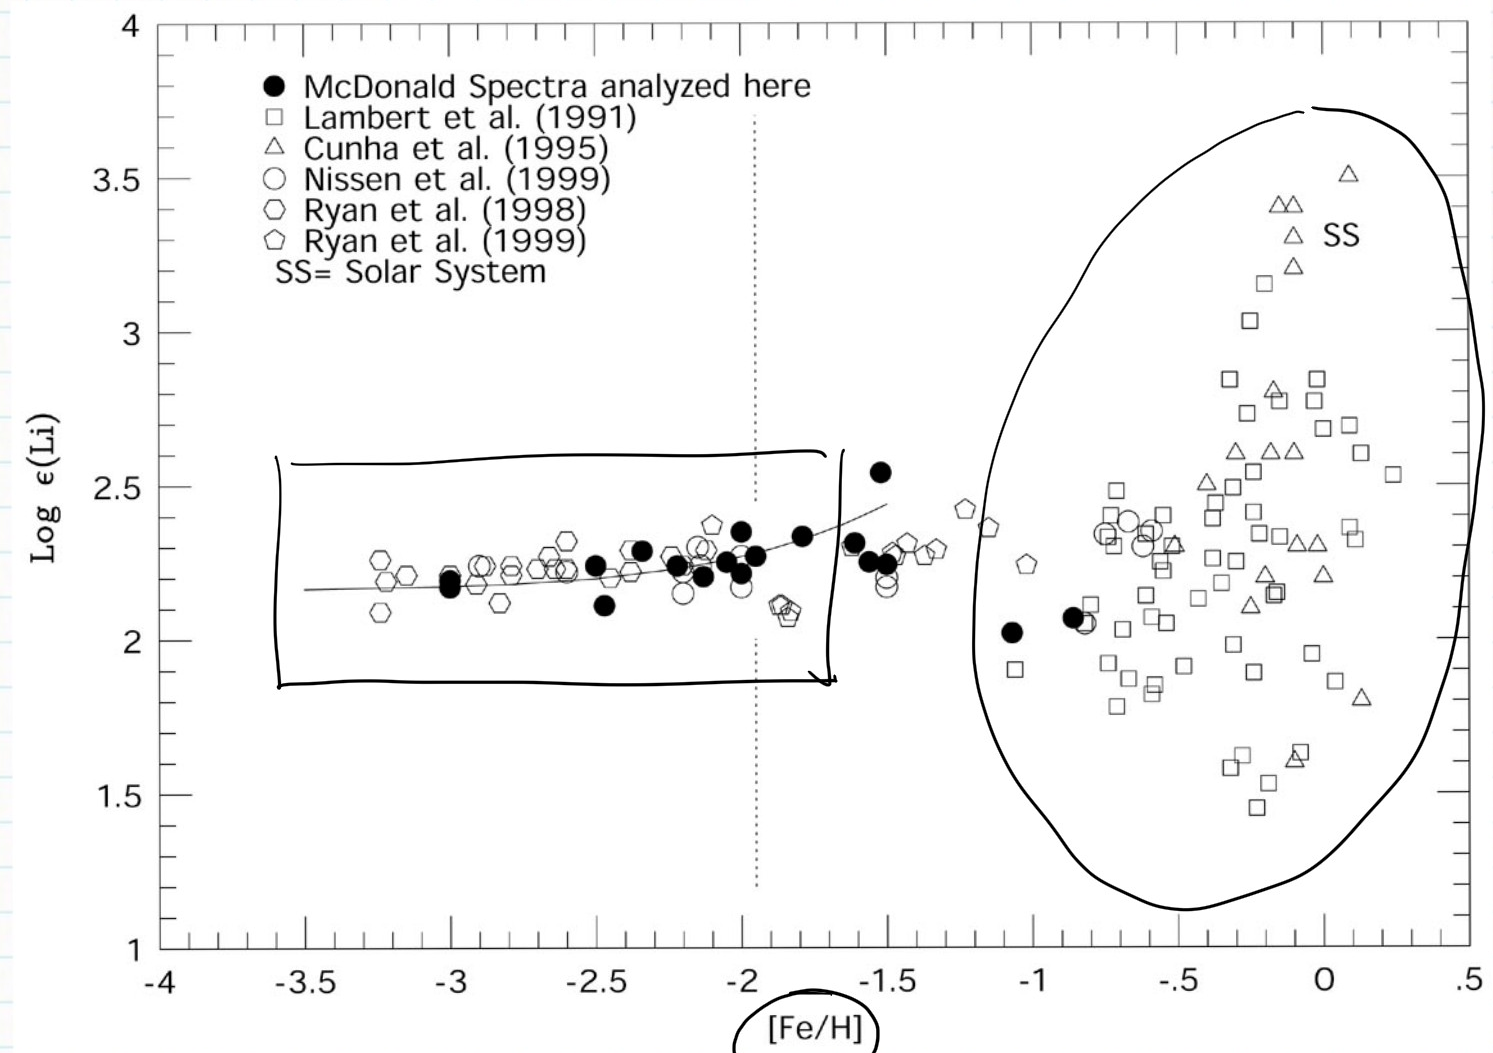
\includegraphics[scale=0.25]{Immagini/0315_LiH.png}
    \caption{\textit{Splite Plateau} per il $\ce{Li}$. Con $\varepsilon (\ce{Li})$ si indica la \textit{mass fraction} del litio.}
    \label{0315_LiH}
\end{figure}
\newpage
\section{La BBN e i neutrini}
Alla fine degli anni '90 la teoria della BBN era ormai supportata dall'accordo con evidenze sperimentali nell'abbondanza di 3 degli elementi più presenti, %
% Compare negli appunti un "per = Omega_B"
per cui aveva acquistato un potere predittivo; essa può essere usata infatti per rielaborare il numero di neutrini o meglio la \textit{radiation density}\index{radiation density@\textit{radiation density} $N_\nu$} $N_\nu$ (l'osservabile che effettivamente si misura). Un aumento delle specie di neutrini, appunto, porterebbe a un aumento nella densità di energia, che regola il rate di espansione (per cui un'espansione più veloce) e quindi ci aspetteremmo che il \textit{Freeze-out}\index{Freeze-out@\textit{Freeze-out}} accada prima: $H^2 \propto N_\nu T^4$, dunque se $N_\nu $ è maggiore allora $T$ è minore. Se riprendiamo l'esempio che avevamo fatto nel paragrafo \vir{\textbf{A grandi linee}} a pg. \pageref{a.grandi.linee} per il numero di neutroni al \textit{Freeze-out} si ha in questo caso:
$$N_n = N_0 e^{-t/\tau} = 220 e^{-100/886} \simeq 196$$
Abbiamo quindi un maggior numero di neutroni e questo comporta una densità di $\ce{^4He}$ più alta. Riportiamo in Figura \ref{0315_Hefrac2} l'andamento della \textit{mass fraction} per l'elio al variare della $N_\nu$.

\begin{figure}[h]
    \centering
    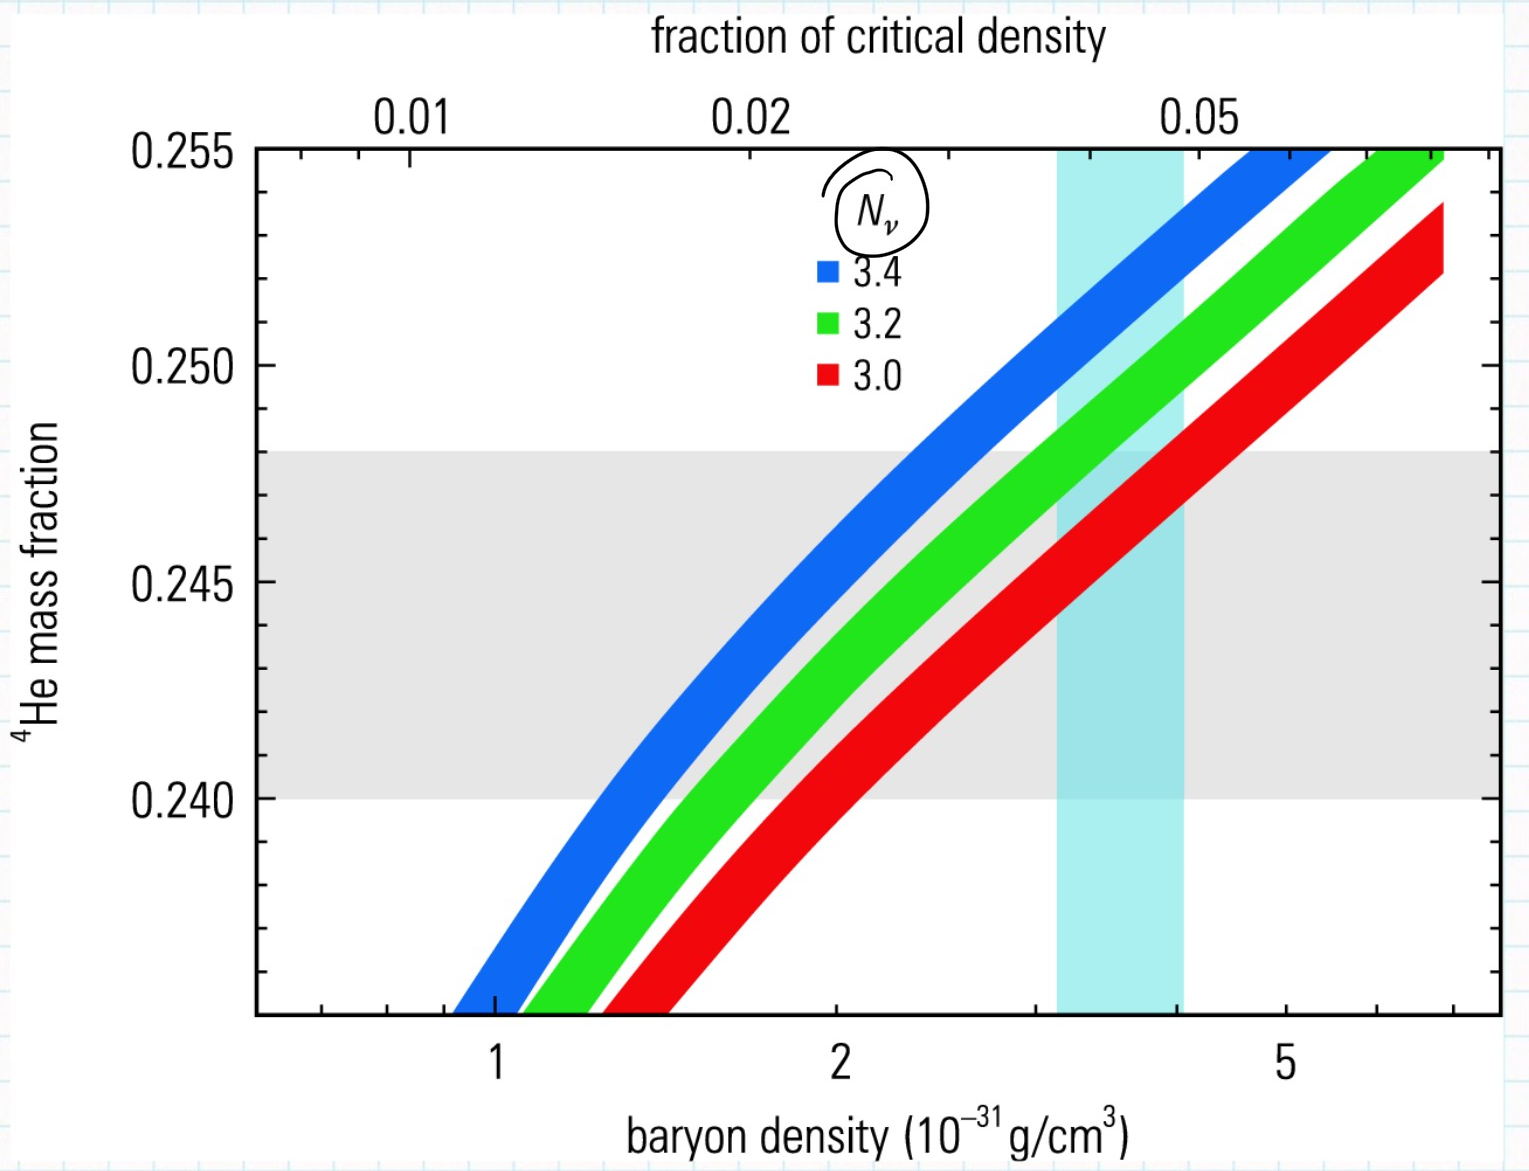
\includegraphics[scale=0.2]{Immagini/0315_heliummassfraction2.png}
    \caption{La banda grigia rappresenta i dati sperimentali. Data la densità dei barioni si evince che gli andamenti per $N_\nu = 3.4$ e $3.2$ vadano esclusi.}
    \label{0315_Hefrac2}
\end{figure}
\section{La BNN oggi}
La teoria della BBN a oggi si basa sul modello cosmologico standard\index{modello cosmologico standard@modello cosmologico standard $\Lambda CDM$} $\Lambda CDM$\footnote{L'acronimo:%
\begin{itemize}
    \item[$\Lambda$] sta per la costante cosmologica\index{costante cosmologica@costante cosmologica $\Lambda$}.
    \item[$CDM$] sta per \textit{Cold Dark Matter}.
\end{itemize}
}.\\
Di recente $\Omega_B h^2$ è stato misurato dal CMB ed è quindi possibile fare delle stime sulle abbondanze; il $d/\ce{H}$, per esempio, che è particolarmente sensibile al valore di $\Omega_B$ e a $N_\nu$\footnote{Da qui in poi chiameremo $N_\nu$ con $N_{eff}$.} e per il quale abbiamo una serie di reazioni che lo creano e lo distruggono\footnote{Fino al 2020 l'ultima era la più incerta.}:
\begin{displaymath}
\begin{aligned}
n + p &\to d + \gamma & &\text{Creazione} \\
d + d &\to \ce{^3He} + n & \\
d + d &\to \ce{^3H}  + p &  &\text{Distruzione} \\
p + d &\to \ce{^3He} + \gamma & 
\end{aligned}
\end{displaymath}
Quello che si misura effettivamente è il \textbf{fattore astrofisico}\index{fattore astrofisico@fattore astrofisico $S(E)$} $S(E)$, che ha le dimensioni di una sezione d'urto per un'energia; si riportano i risultati sperimentali per l'ultima reazione di distruzione in Figura \ref{0315_astr}.

\begin{figure}[h]
    \centering
    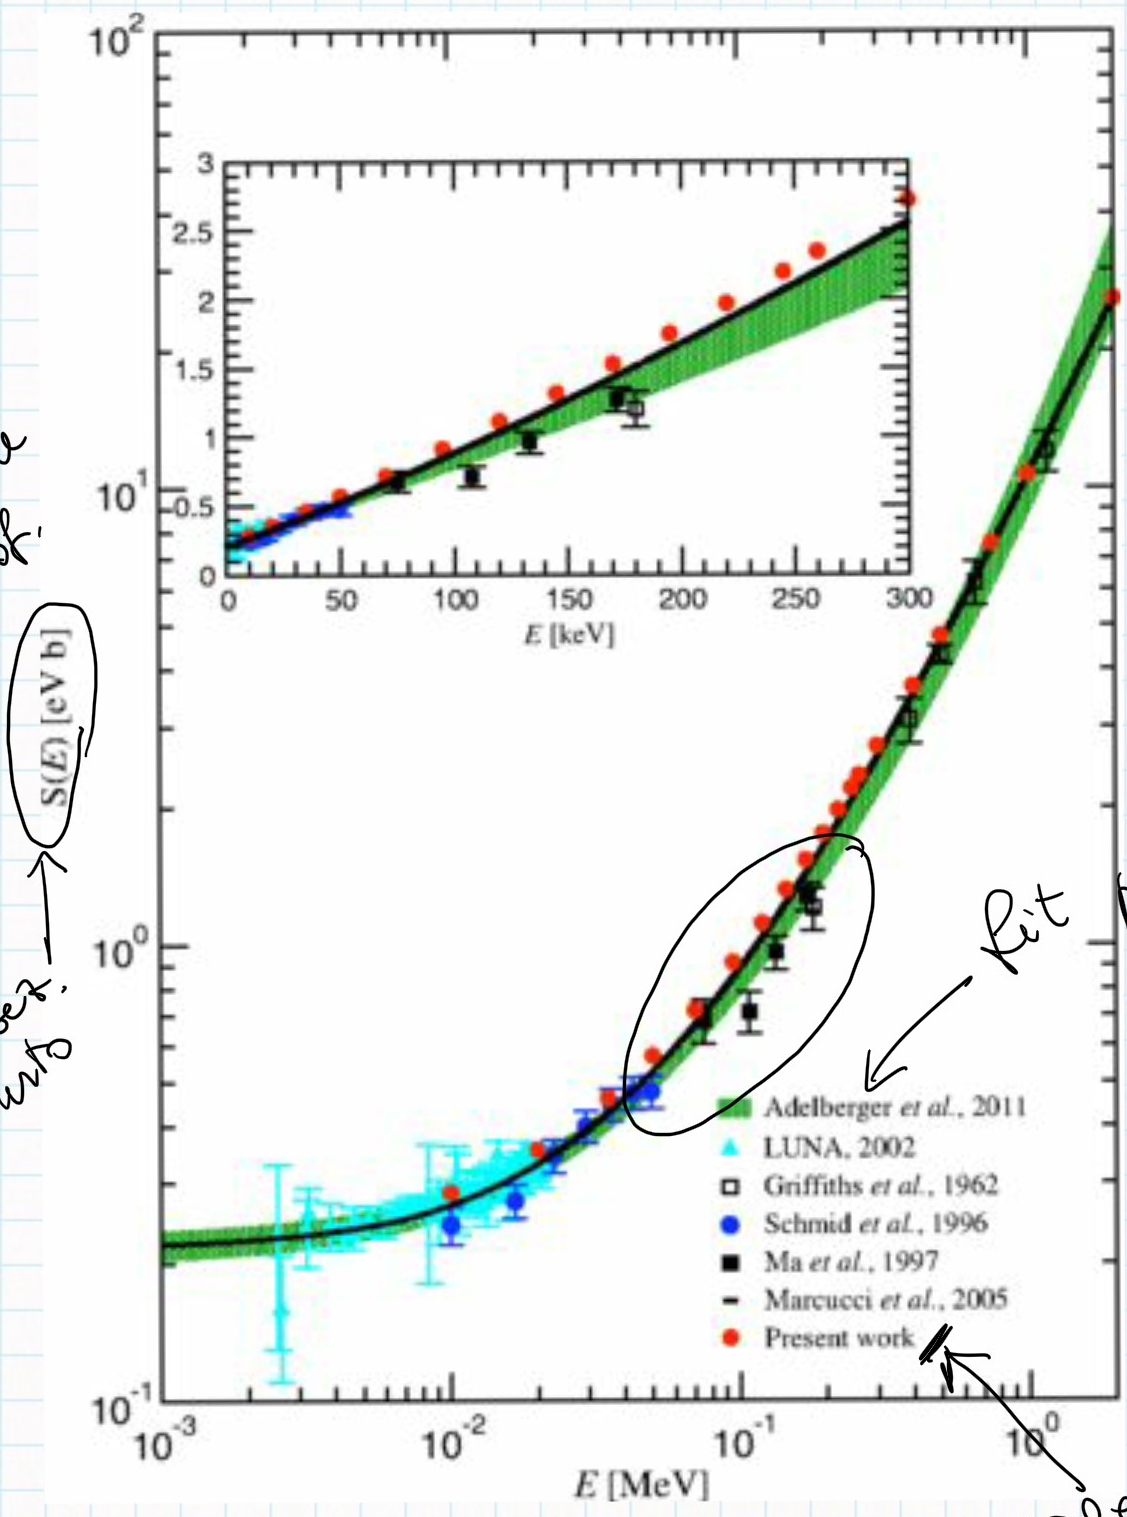
\includegraphics[scale=0.2]{Immagini/0315_fattoreastr.png}
    \caption{La parte cerchiata è il range di interesse per la BBN. La banda verde corrisponde a un fit polinomiale, i punti rossi ad alcuni calcoli teorici e i punti neri ai dati (che rimangono sotto a tutto).}
    \label{0315_astr}
\end{figure}
\newpage
\noindent Recentemente in Italia si sono fatte altre prese dati grazie all'esperimento LUNA\esperimento{LUNA}\footnote{che discuteremo ampiamente nella sezione \secrif{sec-LUNA}.}, che ha raggiunto un'incertezza del 3\%. Riportiamo i risultati in Figura \ref{0315_astr2}. Rispetto al precedente, il rate di presa dati era molto maggiore e le misure molto più accurate, grazie un codice numerico detto \textit{PArthENoPE}\index{PArthENoPE@\textit{PArthENoPE}}\footnote{Per info: \url{http://parthenope.na.infn.it}.}, che ritorna le funzioni di \textit{likehood} riportate in Figura \ref{0315_parthenope}\footnote{La differenza tra il calcolo delle linee segnate come \textit{Marcucci} è dovuta alle funzioni d'onda di scattering; si osserva che le misure del 2016 sono più accurate, tuttavia non se ne conosce il motivo.}.

\begin{figure}[h]
    \centering
    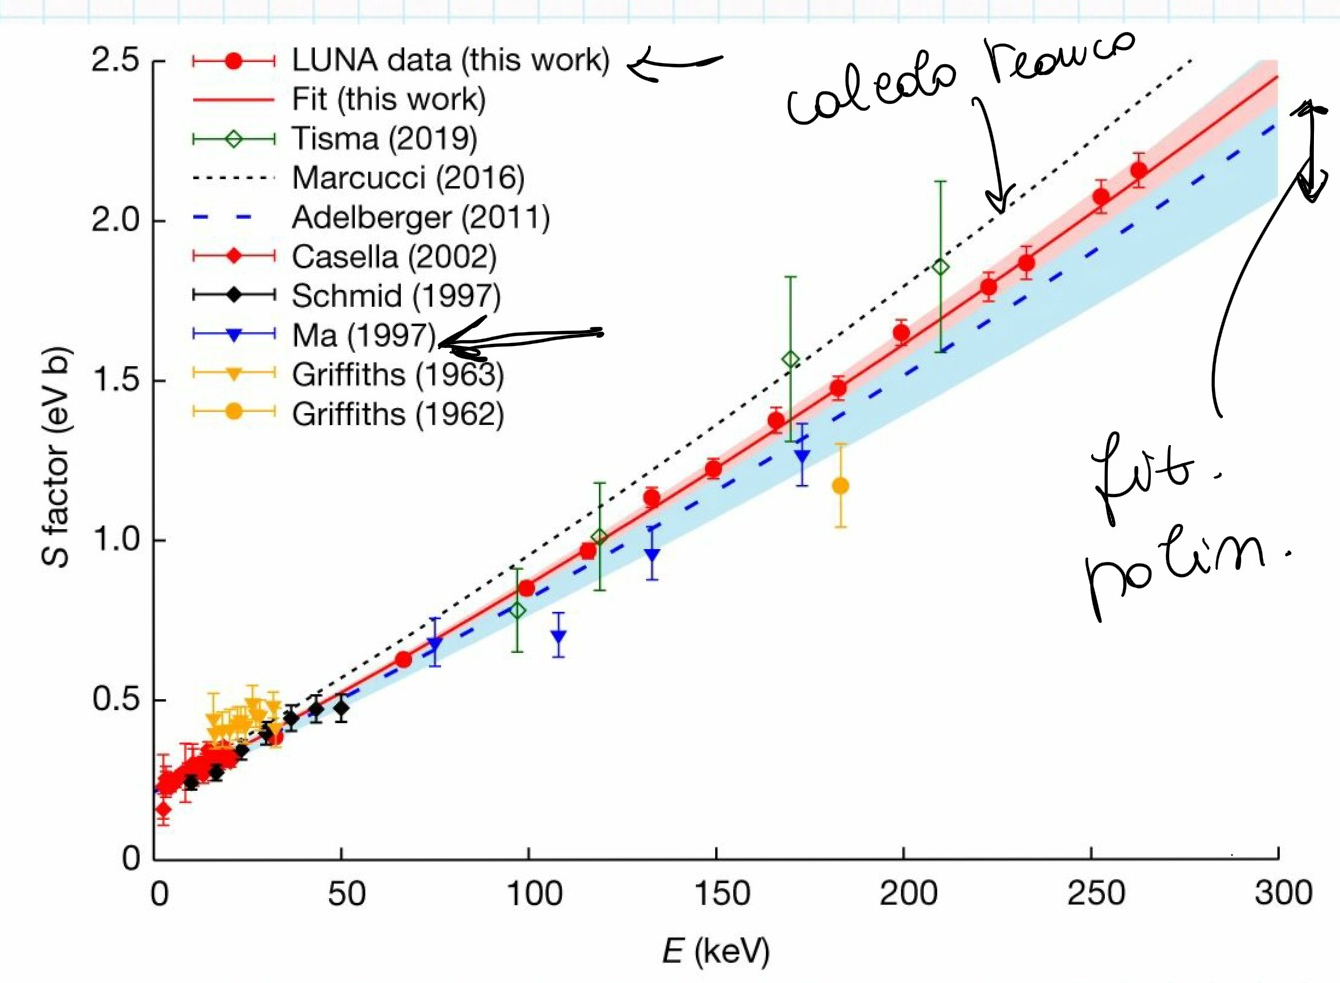
\includegraphics[scale=0.2]{Immagini/0315_fattoreastr2.png}
    \caption{I dati blu sono quelli che nella figura precedente erano segnati in nero. Quelli rossi sono i nuovi dati, la banda celeste corrisponde al fit polinomiale e la linea tratteggiata è l'andamento teorico. I dati di Casella 2002 (basse energie) sono quelli di LUNA I, mentre i dati in rosso circolari sono quelli di LUNA II (vedi \secrif{sec-LUNAII}).}
    \label{0315_astr2}
\end{figure}



\begin{figure}[!h]
    \centering
    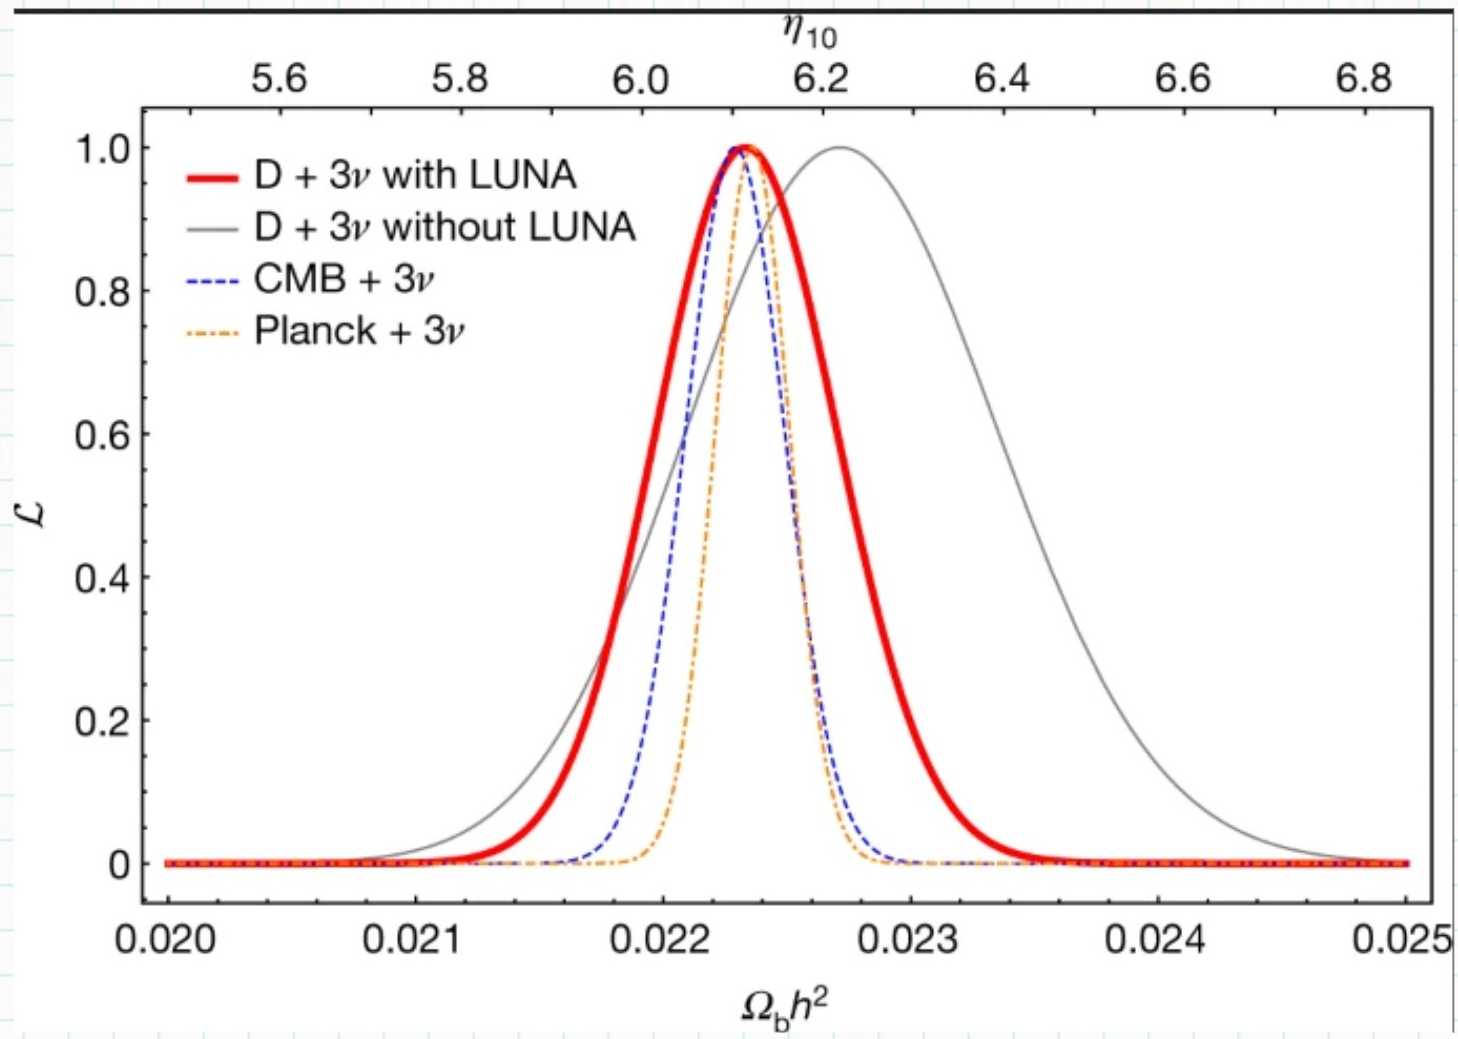
\includegraphics[scale=0.2]{Immagini/0315_luna.png}
    \caption{Risultati per i vari esperimenti ottenuti tramite \textit{PArthENoPE}.}
    \label{0315_parthenope}
\end{figure}
\newpage
\noindent Dato $\Omega_B h^2$ da Planck, è possibile predire $d/\ce{H}|_\text{BBN} = (2.52\pm0.03\pm0.06)\cdot\ord{-5}$ da confrontare con il valore $\Omega_B$ più probabile ottenuto attraverso l'algoritmo. Riportiamo in Figura \ref{0315_risultati} i risultati di LUNA, che hanno mostrato come non ci sia \textit{nuova fisica} in questo campo: vi è un forte accordo tra il modello standard $\Lambda CDM$ e la teoria della BBN.\\
Rimane ancora in sospeso il $\ce{Li}$-\textit{problem}\index{Li-problem@$\ce{Li}$-\textit{problem}}\index{Li-puzzle@$\ce{Li}$-\textit{puzzle}}, ma le ipotesi più recenti sostengono che probabilmente sia dovuto a un errore nella misurazione dell'abbondanza primordiale del litio.



\begin{figure}[h]
    \centering
    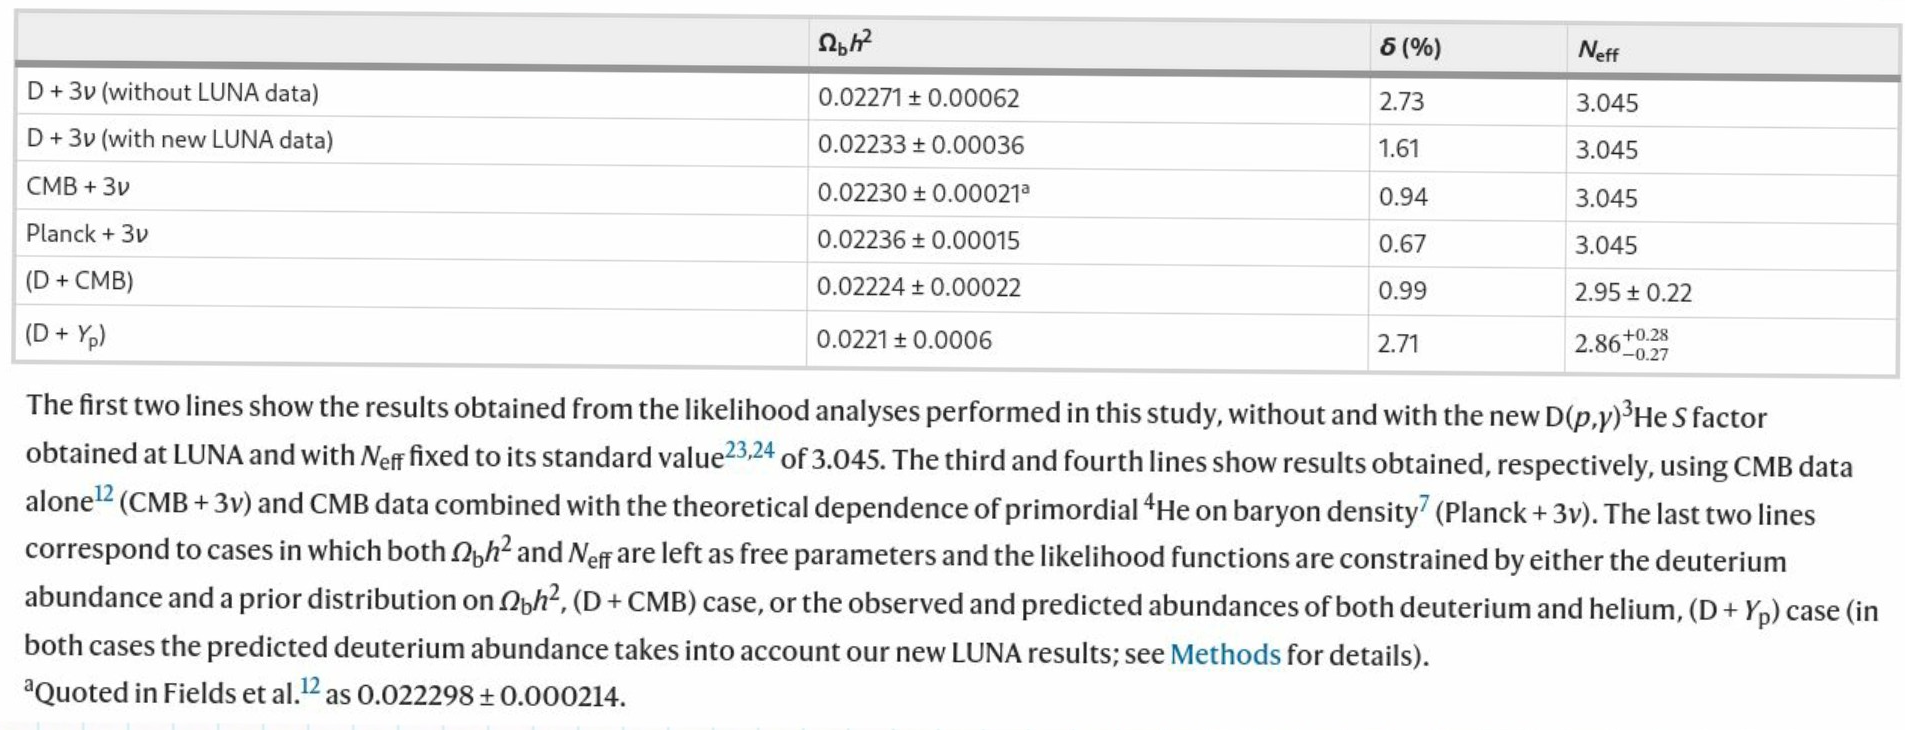
\includegraphics[scale=0.26]{Immagini/0315_risultati.png}
    \caption{Risultati di LUNA. Nei casi delle ultime due righe è stata rilasciato il numero di neutrini, precedentemente fissato dall'abbondanza di elio.}
    \label{0315_risultati}
\end{figure}    %   15/03
%%  La prima reazione
%\part*{Lezione 17/03/2021}
\section{La prima reazione}\label{0317-sec-abinitio}
Dopo il decadimento del neutrone, la prima reazione che avviene (secondo la Figura \ref{0315_net}) è:
$$p + n \to d + \gamma$$
Tra le reazioni del network questa è la più \vir{semplice}, ovvero $A=2$. 

\subsection{Cinematica} 
Studiamo allora la sezione d'urto di questa reazione:
$$d\sigma \overset{\text{Reg. d'Oro}}{=} \frac{\text{Rate di transizione}}{\text{Flusso incidente}} = \frac{\lambda}{v_{rel}}$$
Concentriamoci sulla probabilità di transizione $W_{i\to f}$, mettendoci nel sistema del centro di massa\footnote{Usiamo la solita convenzione $c=\hbar = 1$, la notazione $\vec{q}$ per l'impulso del fotone e $\vec{P}_d$ per quello del deuterio e assumiamo volumi unitari.}.
$$W_{i\to f} = |V_{i\to f}|^2\:dn \qquad \text{con   } dn = \frac{d^3q}{(2\pi)^3}\frac{d^3P_d}{(2\pi)^3} (2\pi)^3 \delta^3(\vec{P}_d+\vec{q}) \Rightarrow \frac{d^3q}{(2\pi)^3}$$
dove $V_{i\to f}$ è l'elemento di matrice di transizione, $T$ è il tempo di interazione e $dn$ è l'elemento infinitesimo di spazio delle fasi (in cui abbiamo risolto per la $\delta$). Dalla teoria perturbativa al primo ordine\footnote{Dove $T$ è un tempo molto maggiore rispetto a quelli di evoluzione del sistema.}:
$$V_{i\to f} = -i \int_0^T \oss{f}{V(t)}{i}\, e^{i(E_f-E_i)t} dt \qquad \text{dove } V(t) = -e \vec{A}(\vec{x}) \cdot \vec{J}(\vec{x}) $$
\begin{displaymath}
\begin{aligned}
\oss{f}{V(t)}{i} &= - e\int d^3x \; \oss{\gamma}{\vec{A}(\vec{x})}{0} \cdot \oss{d(\vec{P}_d,\sigma_d)}{\vec{J}(\vec{x})}{pn} = \\
&= -e \int \frac{\widehat{\varepsilon}^*(\vec{q},\lambda)}{\sqrt{2q}} \cdot \underbrace{e^{-i\vec{q}\cdot\vec{x}}\oss{d}{\vec{J}(\vec{x})}{pn}\: d^3x}_{\text{Definiamo questo } \vec{J}^+(\vec{q})} = \\
&= -\frac{e}{\sqrt{2q}} \, \widehat{\varepsilon}^*(\vec{q},\lambda) \cdot \vec{J}^+(\vec{q})
\end{aligned}
\end{displaymath}
dove\footnote{Si è fatto uso di un abuso di notazione esplicitando l'integrale racchiuso dal braket. Spesso faremo questo abuso per esplicitare su quale variabile integriamo.} abbiamo assunto $\omega = E = q$. Per cui sostituendo:
\begin{align*}
    V_{i\to f} &= \frac{ie}{\sqrt{2q}}\,\widehat{\varepsilon}^*(\vec{q},\lambda) \cdot \vec{J}^+(\vec{q})\, \int_0^T dt \, e^{i(E_f-E_i)t} = \\
    &= \frac{ie}{\sqrt{2q}}\,\widehat{\varepsilon}^*(\vec{q},\lambda) \cdot \vec{J}^+(\vec{q})\,\frac{2\sin{(T (E_f-E_i)/2)}}{(E_f-E_i)} \, e^{i(E_f-E_i)T/2}
\end{align*}
$$\frac{|V_{f\to i}|^2}{T} = \frac{e^2}{2q} |\widehat{\varepsilon}^*(\vec{q},\lambda) \cdot \vec{J}^+(\vec{q})|^2\, 2\pi \delta(E_f - E_i)$$
La $\delta$ rappresenta la conservazione dell'energia\footnote{La funzione $\sin^2(xT)/x^2 \to \pi T \delta$ per $T\to\infty$; dunque $T\gg \hbar/(E_f-E_i)$ come avevamo assunto.}.\\
Possiamo allora scrivere la sezione d'urto differenziale:
\begin{displaymath}
\begin{aligned}
d\sigma &= \frac{e^2}{2} |\widehat{\varepsilon}^*(\vec{q},\lambda) \cdot \vec{J}^+(\vec{q})|^2\, q dq \frac{d\Omega_{\hat{q}}}{(2\pi)^2}\, \delta(E_f - E_i) \frac{1}{v_{rel}} \\
\frac{d\sigma}{d\Omega_{\hat{q}}} &= \frac{e^2}{8\pi^2} |\widehat{\varepsilon}^*(\vec{q},\lambda) \cdot \vec{J}^+(\vec{q})|^2\, q dq \, \delta(E_p + E_n - m_d - \frac{q^2}{2m_d}-q) \frac{1}{v_{rel}}
\end{aligned}
\end{displaymath}
Poiché vogliamo che la sezione d'urto sia mediata su tutte le polarizzazioni sommiamo su tutte quelle finali $\sum_{\lambda=\pm 1 ,\; \sigma_d = \pm 1, 0}$ e mediamo su quelle iniziali $\frac{1}{4}\sum_{s_n,s_p = \pm \frac{1}{2}}$, per cui:
$$\frac{d\sigma}{d\Omega_{\hat{q}}} = \frac{e^2}{4\pi}\frac{1}{8\pi v_{rel}}\sum_{\lambda=\pm 1 ,\; s_d = \pm 1, 0} \sum_{s_n,s_p = \pm \frac{1}{2}} \int q dq |\widehat{\varepsilon}^*(\vec{q},\lambda) \cdot \vec{J}^+(\vec{q})|^2\,\frac{\delta (q-\bar{q})}{1+\frac{\bar{q}}{m_d}}$$
$$\frac{d\sigma}{d\Omega_{\hat{q}}}=\frac{e^2}{4\pi}\frac{1}{8\pi v_{rel}}\sum_{\lambda=\pm 1 ,\; s_d = \pm 1, 0} \sum_{s_n,s_p = \pm \frac{1}{2}}  |\widehat{\varepsilon}^*(\vec{\bar{q}},\lambda) \cdot \vec{J}^+(\vec{\bar{q}})|^2\,\frac{\bar{q}}{1+\frac{\bar{q}}{m_d}}$$
dove abbiamo usato la proprietà della $\delta$\footnote{$$\delta (f(q)) = \sum_{i=0}^N\frac{\delta(q-\bar{q}_i)}{|f'(\bar{q}_i)|}$$
con $\bar{q}_i$ zeri della funzione $f$.}, per cui $\bar{q} = m_d \ppc{-1+ \sqrt{1+2\Delta E/m_d}}$ con $\Delta E = E_p + E_n - m_d \overset{\text{CM}}{=} m_n+m_p-m_d + T_{rel}$. Notiamo che questa espressione è simile a quella del decadimento $\gamma$, infatti questo formalismo\footnote{Ovvero potremo sempre scrivere ${d\sigma}/{d\Omega_{\hat{q}}} \propto 1/(8\pi v_{rel})\; \sum \sum \, |\dots|^2\, {\bar{q}}/{(1+\bar{q}/m_c)}$.} vale per ogni decadimento del tipo $a+b\to c +\gamma$.\\
Notiamo che $\sigma \propto 1/v_{rel} \sim 1/\sqrt{T_{rel}}$ ed è quindi l'energia cinetica relativa che fa da discrimine per far avvenire la reazione; questo andamento si ritrova in generale a basse energie per $n+a$.

\subsection{Funzioni d'onda} 
Finora abbiamo trattato solo la cinematica della reazione, per continuare è necessario sviluppare le funzioni d'onda\footnote{Da qui in poi, ovviamente, i risultati trovati non varranno per ogni $a+b\to c +\gamma$.}.
\begin{displaymath}
\begin{aligned}
&\Bigl|\widehat{\varepsilon}^*(\vec{q},\lambda) \cdot \vec{J}^+(\vec{q})\Bigr|^2 = \\
=& \Bigl|\oss{d}{\int d^3x \; e^{-i\vec{q}\cdot\vec{x}}\widehat{\varepsilon}^*(\vec{q},\lambda) \cdot \vec{J}(\vec{x})}{pn}\Bigr|^2 \equiv\\
\equiv& \Bigl | \widehat{\varepsilon}^*(\vec{q},\lambda) \cdot \oss{\psi_{1s_d}}{\vec{J}_\lambda(\vec{q})}{\psi_{s_p s_n}(\vec{p})} \Bigr |^2 \\
\vec{J}_\lambda(\vec{q}) \equiv&\int d^3x \; e^{-i\vec{q}\cdot\vec{x}}\vec{J}(\vec{x})
\end{aligned}
\end{displaymath}
per $\psi_{s_p s_n}(\vec{p})$ ci aspetteremo dei multipoli come avevamo visto nel decadimento $\gamma$. Per $\widehat{\varepsilon}$ consideriamo polarizzazione circolare:
$$\widehat{\varepsilon}(\lambda) = \mp \frac{\widehat{e}_x \pm i\,\widehat{e}_y}{\sqrt{2}}\qquad \text{con } \vec{q} // \hat{z} $$
Dato che il momento $\vec{J}$ per gli stati iniziali non è ben definito non possiamo usare immediatamente l'espansione in multipoli, per cui prima sviluppiamo le funzioni d'onda in onde parziali\index{sviluppo in onde parziali}\footnote{Per non confondere $J$ corrente con $J$ momento denoteremo quest'ultimo con la lettera $\Lambda$.}:
\begin{displaymath}
\begin{aligned}
\psi_{s_ps_n}(\vec{p}) &= 4\pi \sum_{S,S_z} \clebs{\frac{1}{2}s_n,\,\frac{1}{2}s_p}{S\,S_z}\, \sum_{L,Lz,\Lambda,\Lambda_z} \clebs{SS_z,\,LL_z}{\Lambda\,\Lambda_z} i^L \mathcal{Y}^*_{LL_z}(\widehat{p}) \, \psi_{np}^{(LS\Lambda\Lambda_z)} \\
%
\oss{\psi_{1s_d}}{J_\lambda(\vec{q})}{\psi_{s_p s_n}(\vec{p})} &= 4\pi \,(\dots)\, \oss{\psi_{1s_d}}{J_\lambda(\vec{q})}{\psi_{np}^{(LS\Lambda\Lambda_z)}}
\end{aligned}
\end{displaymath}
$\psi_{np}^{(LS\Lambda\Lambda_z)}$ ha $\Lambda$ ben definito, quindi è un'ottima candidata per l'espansione in multipoli. Poiché le energie sono basse\footnote{Stiamo considerando una cattura termica\index{cattura termica} con neutroni, appunto, termici.}, possiamo allora considerare solo $\ce{^1S_0}$ ($S=L=\Lambda = 0$), ovvero le onde sferiche\index{armoniche sferiche}:
\begin{displaymath}
\begin{aligned}
\psi_{s_p s_n}(\vec{p}) &= 4\pi \clebs{\frac{1}{2}s_n\,\frac{1}{2}s_p}{00}\, \underbrace{\frac{1}{\sqrt{4\pi}}}_\text{Arm. sfer.} \, \psi_{np}(\ce{^1S_0}) \\
%
\oss{\psi_{1s_d}}{J_\lambda(\vec{q})}{\psi_{s_p s_n}(\vec{p})} &\equiv \sqrt{4\pi} \clebs{\frac{1}{2}s_n\,\frac{1}{2}s_p}{00}\, j^{\ce{^1S_0}}_{\lambda s_d} (\vec{q}) \\
j^{\ce{^1S_0}}_{\lambda s_d} (\vec{q}) &\equiv \oss{\psi_{1s_d}}{\int d^3x \; e^{-i\vec{q}\cdot\vec{x}}\widehat{\varepsilon}^*(\vec{q},\lambda) \cdot \vec{J}(\vec{x})}{\psi_{np}(\ce{^1S_0})} = \\
&= -\sqrt{2\pi} \sum_{\Lambda'\geq 1} (-i)^{\Lambda'} \sqrt{2\Lambda' +1} \oss{\psi_{1s_d}}{E_{\Lambda'-\lambda}(q)  + \lambda \, M_{\Lambda'-\lambda}(q)}{\psi_{np}(\ce{^1S_0})}
\end{aligned}
\end{displaymath}
dove abbiamo prima definito $j^{\ce{^1S_0}}_{\lambda s_d} (\vec{q})$ e poi sviluppato in multipoli come nel decadimento $\gamma$\footnote{Guarda \secrif{sec-gamma-multipoli}.} (chiamando $\Lambda'$ l'ordine del multipolo per distinguerlo da $\Lambda$).
La parità\footnote{Qui con $J$ si indica il momento angolare totale e con $\Lambda$ quello del fotone e quindi l'ordine di multipolo.} dei singoli termini è data da $\pi(E\Lambda)=(-1)^\Lambda$ e $\pi(M\Lambda)=(-1)^{\Lambda+1}$, per cui, poiché deve valere $\vec{\Lambda}+\vec{J}_i = \vec{J}_f$, per $J_f = 1$, $J_i = 0$ e $\pi_i=\pi_f=+$ allora $\Lambda = 1$ e solo $M1$ sarà rilevate ai fini del calcolo al primo ordine:
\begin{displaymath}
\begin{aligned}
\sqrt{4\pi} \clebs{\frac{1}{2}s_n\,\frac{1}{2}s_p}{00}\, j^{\ce{^1S_0}}_{\lambda s_d} (\vec{q}) &\simeq \sqrt{4\pi} \clebs{\frac{1}{2}s_n\,\frac{1}{2}s_p}{00}\: \oss{\psi_{1s_d}}{-\sqrt{2\pi}(-i) \sqrt{3} (\lambda\,M_{1-\lambda}(q))}{\psi_{np}(\ce{^1S_0})}\\
j^{\ce{^1S_0}}_{\lambda s_d} (\vec{q})&\simeq i\sqrt{6\pi} \lambda \oss{\psi_{1s_d}}{M_{1\,-\lambda}}{\psi_{np}(\ce{^1S_0})} =\\
&= i \sqrt{6\pi} \lambda \:\underbrace{ \frac{\clebs{00,1-\lambda}{1s_d}}{\sqrt{3}}}_\text{Dal teo. di W-E} \: \underbrace{\bigl \langle \, \psi_{1s_d}\,||\,M_1\,||\,\psi_{np}(\ce{^1S_0})\rangle}_\text{El. di matrice ridotta} = \\
&= i \sqrt{2\pi} \lambda \: \delta_{-\lambda s_d} \: |M_1(q)|
\end{aligned}
\end{displaymath}
dove abbiamo applicato il teorema di \WE\index{teorema di \WE}. Il segno di $\lambda$ non è importante in questa trattazione perché siamo interessati alla somma su tutte le polarizzazioni (per cui $\sum_{\lambda=\pm 1}$):
$$\sum_{s_ns_p,\lambda s_d}|\sqrt{4\pi} \clebs{\frac{1}{2}s_p\,\frac{1}{2}s_n}{00}\, j^{\ce{^1S_0}}_{\lambda s_d} (\vec{q})|^2 = 4\pi \underbrace{\sum_{s_ns_p}|\clebs{\frac{1}{2}s_p\,\frac{1}{2}s_n}{00}|^2}_{=1} \; \sum_{\lambda s_d} 2\pi \delta_{\lambda s_d}\,|M_1|^2 = 16\pi^2 |M_1|^2$$
dove abbiamo usato $\sum_{\lambda s_d}\delta_{\lambda s_d}=\delta_{11} + \delta_{-1-1} =2$. Dobbiamo calcolare $M_1(q)$, ma dal momento che questo non dipende da $\lambda$ possiamo stimarlo per qualsiasi valore di $\lambda$ (per esempio $\lambda = -1$):
\begin{displaymath}
\begin{aligned}
j^{\ce{^1S_0}}_{\lambda,-\lambda} &= i \sqrt{2\pi} \lambda M_1(q)\\
M_1(q) &= \frac{-i}{\sqrt{2\pi}} j^{\ce{^1S_0}}_{-11} (\vec{q}) \\
\frac{d\sigma}{d\Omega_{\hat{q}}} &\propto \frac{1}{v_{rel}} \frac{\bar{q}}{1+\bar{q}/m_d} \, |j^{\ce{^1S_0}}_{-11}(\vec{\bar{q}})|^2 \\
\sigma_{tot} &= \int \frac{d\sigma}{d\Omega_{\hat{q}}} d\Omega_{\hat{q}} \propto \frac{4\pi}{v_{rel}} \frac{\bar{q}}{1+\bar{q}/m_d} |j^{\ce{^1S_0}}_{-11}(\vec{\bar{q}})|^2
\end{aligned}
\end{displaymath}
Abbiamo così isolato la parte nucleare e il problema si riduce al calcolo di $j^{\ce{^1S_0}}_{-11}$:
$$j^{\ce{^1S_0}}_{-11} = \int d^3r_1 d^3r_2 \;\: \psi_{11}^*(\vec{r}_1,\vec{r}_2)\: \widehat{\varepsilon}^*(\vec{q},-1) \cdot\vec{J}_{-1}\:\psi^{\ce{^1S_0}}(\vec{r}_1,\vec{r}_2)$$
A questo punto abbiamo bisogno della funzione d'onda del deutone, di quella di scattering $np$, del potenziale nucleare e di un metodo numerico che risolva l'equazione di \Sch{} sia per lo stato legato che per quello di scattering. Questo non è però sufficiente, è necessario anche un modello per la corrente elettromagnetica\footnote{Attenzione: in $J_{\lambda,i}$ l'indice $i$ indica l'$i$-esimo nucleone e non ha niente a che vedere con il momento angolare totale iniziale. Si invita il lettore da qui in poi a cercare di capire dal contesto il significato delle notazioni.} e ne avevamo uno:\index{corrente di convezione}
$$\vec{J}_{\lambda,i} = \frac{1}{2m} \underbrace{\varepsilon_i \PPg{\vec{p}_i,\:e^{i\vec{q}\cdot\vec{r}_i}}}_\text{corrente di convezione} - \frac{i}{2m} \mu_i \, \vec{q}\times \vec{\sigma}_i\, e^{i\vec{q}\cdot\vec{r}_i}$$
$$\varepsilon_i \simeq \frac{1}{2}(1+\tau_{z,i})$$
$$\mu_i \simeq \frac{1}{2}(1+\tau_{z,i})\mu_p + \frac{1}{2}(1-\tau_{z,i})\mu_n = \frac{1}{2} (\mu_S +\mu_V \tau_{z,i}) $$
dove $\varepsilon_i$ e $\mu_i$ sono proiettori e $\mu_S = \mu_p + \mu_n = 0.88\: \mu_N $ e $\mu_V = \mu_p - \mu_n = 4.706 \: \mu_N$ sono rispettivamente la combinazione isoscalare\index{combinazione isoscalare} e quella vettoriale \index{combinazione vettoriale}. In generale, l'integrale scritto precedentemente per $j_{-11}^{\ce{^1S_0}}$ viene risolto numericamente in $d^3r_{rel}d^3r_{CM}$, ma dal momento che siamo interessati alla soluzione analitica e ci troviamo nel caso di basse energie (cattura di neutroni termici, quindi $\vec{p}_i\sim 0$, corrente di convezione\index{corrente di convezione} trascurabile) possiamo studiare solo l'onda $s$\footnote{Abbiamo indicato con $\chi$ la funzione di \textit{spin} e con $\zeta$ quella di \textit{isospin}:%
\begin{displaymath}
\begin{aligned}
\zeta_{00} &= \frac{\ket{np}-\ket{pn}}{\sqrt{2}} & \chi_{11} &= \ket{\uparrow\uparrow} \\
\zeta_{10} &= \frac{\ket{np}+\ket{pn}}{\sqrt{2}} & \chi_{00} &= \frac{\ket{\downarrow\uparrow}-\ket{\uparrow\downarrow}}{\sqrt{2}} 
\end{aligned}
\end{displaymath}%
}:
$$\psi_{11} = \underbrace{\PPq{\frac{1}{\sqrt{4\pi}}\frac{u(r)}{r}\chi_{11}\zeta_{00}}}_\text{deutone fermo}\, \underbrace{e^{-i\vec{p}_d\cdot\vec{R}}}_\text{moto}$$
$$\psi^{\ce{^1S_0}} = \PPq{\frac{1}{\sqrt{4\pi}}\frac{u_S(r)}{r}\chi_{00}\zeta_{10}}\, e^{-i\vec{p}_{CM}\cdot\vec{R}}$$
La corrente sarà quindi data da:
$$\vec{J}_i \simeq -\frac{i}{2m} \mu_i\: \vec{q}\times \vec{\sigma}_i\, e^{i\vec{q}\cdot \vec{r}_i}$$
Notiamo che $\zeta_{00}^+\, \mu_S\, \zeta_{10} = 0$ perché le due funzioni sono ortogonali fra loro, dunque sopravvive solo il pezzo con $\mu_V$ nella corrente:
$$\vec{J}_{\lambda=-1} = -\frac{i}{4m} \mu_V \PPq{(\vec{q}\times\vec{\sigma}_1)_{\lambda=-1} e^{i\vec{q}\cdot\vec{r}_1}\tau_{z,1} + (\vec{q}\times\vec{\sigma}_2)_{\lambda=-1} e^{i\vec{q}\cdot\vec{r}_2}\tau_{z,2}} $$
Studiamo adesso la componente del prodotto vettoriale:
\begin{displaymath}
\begin{aligned}
(\vec{q}\times\vec{\sigma}_i)_{\lambda=-1} &= \widehat{\varepsilon}_{\lambda=-1}^* \cdot \vec{q}\times\vec{\sigma}_i =\\
&= -(\widehat{\varepsilon}_{\lambda=+1} \times \vec{q})\cdot\vec{\sigma}_i =\\
&=-(-\frac{\hat{e}_x + i\hat{e}_y}{\sqrt{2}} \times q\hat{e}_z)\cdot\vec{\sigma}_i =\\
&= i \frac{q}{\sqrt{2}} (\hat{e}_x + i\hat{e}_y)\cdot (\sigma_{x,i}\,\hat{e}_x + \sigma_{y,i}\,\hat{e}_y)=\\
&= i \frac{q}{\sqrt{2}}\, \sigma_{+,i} =\\
&= i \sqrt{2} q \, s_{+,i} 
\end{aligned}
\end{displaymath}
dove abbiamo sostituito $\sigma_x + i \sigma_y = \sigma_+ = 2s_+$ operatore di salita\index{operatore di salita}\footnote{Ricordiamo che:%
\begin{displaymath}
\begin{aligned}
s_{+}\ket{\downarrow} &= \ket{\uparrow} & \tau_z \ket{p} &= \ket{p} \\
s_{+}\ket{\uparrow} &= 0 & \tau_z \ket{n} &= -\ket{n}
\end{aligned}
\end{displaymath}%
}; per la corrente avremo allora:
$$\vec{J}_{\lambda=-1} = \frac{q\sqrt{2}}{4m} \mu_V \PPq{e^{i\vec{q}\cdot\vec{r}_1}s_{+,1}\,\tau_{z,1} + e^{i\vec{q}\cdot\vec{r}_2}s_{+,2}\,\tau_{z,2}} $$
Nel calcolo di $j^{\ce{^1S_0}}$ abbiamo:
\begin{displaymath}
\begin{aligned}
j^{\ce{^1S_0}}_{-11}(\vec{q}) = \int d^3r_1d^3r_2\; \frac{1}{4\pi}\frac{u(r)}{r}\frac{u_S(r)}{r}\ppc{\frac{\mu_V\sqrt{2}q}{4m}}e^{i(\vec{p}_d-\vec{p}_{CM})\cdot \vec{R}} &\Bigl [ \chi_{11}^+\zeta_{00}^+\, s_{+,1} \tau_{z,1}\, \chi_{00}\zeta_{10}\:e^{i\vec{q}\cdot\vec{r}_1} \\
&+ \chi_{11}^+\zeta_{00}^+\, s_{+,2} \tau_{z,2}\, \chi_{00}\zeta_{10}\:e^{i\vec{q}\cdot\vec{r}_2}\Bigr ]
\end{aligned}
\end{displaymath}
\begin{displaymath}
\begin{aligned}
\zeta_{00}^+\, \tau_{z,1}\, \zeta_{10} &= \frac{-1-1}{2} =-1  & \chi_{11}^+\, s_{+,1}\, \chi_{00} &= \frac{1}{\sqrt{2}} \\
\zeta_{00}^+\, \tau_{z,2}\, \zeta_{10} &= \frac{1+1}{2} = 1 & \chi_{11}^+\, s_{+,2}\, \chi_{00} &= -\frac{1}{\sqrt{2}} 
\end{aligned}
\end{displaymath}
$$j^{\ce{^1S_0}}_{-11}(\vec{q}) = \int d^3r_1d^3r_2\; \frac{1}{4\pi}\frac{u(r)}{r}\frac{u_S(r)}{r}\ppc{\frac{\mu_V\sqrt{2}q}{4m}}e^{i(\vec{p}_d-\vec{p}_{CM})\cdot \vec{R}}(-\frac{1}{\sqrt{2}})(e^{i\vec{q}\cdot\vec{r}_1}+e^{i\vec{q}\cdot\vec{r}_2})$$
dove $u(r)$ è la funzione ridotta del deutone e $u_S(r)$ è quella della funzione di scattering. Cambiamo variabili\footnote{$\vec{R}=(\vec{r}_1+\vec{r}_2)/2$ e $\vec{r}=\vec{r}_1-\vec{r}_2$.} per cui $\vec{r}_1 = \vec{R}+\vec{r}/2$ e $\vec{r}_2 = \vec{R}-\vec{r}/2$:
$$j^{\ce{^1S_0}}_{11}(\vec{q}) = \int d^3Rd^3r\; \frac{1}{4\pi}\frac{u(r)}{r}\frac{u_S(r)}{r}\ppc{\frac{\mu_V q}{4m}}\: \underbrace{e^{i(\vec{p}_d-\vec{p}_{CM}+\vec{q})\cdot \vec{R}}}_{\delta \text{ per } \vec{p}_d-\vec{p}_{CM}+\vec{q}}\:
\PPq{e^{i\vec{q}\cdot\vec{r}/2}+e^{-i\vec{q}\cdot\vec{r}/2}}$$
L'ultimo termine tra parentesi è simmetrico rispetto a parità $\vec{r}\to -\vec{r}$ e dal momento che la funzione del deutone si annulla per grandi raggi allora $\mean{\vec{q}\cdot\vec{r}}\sim 0$ e quindi $\exp{(i\vec{q}\cdot\vec{r}/2)}\sim 1$.
% $$j^{\ce{^1S_0}}_{-11}(\vec{q}) = \frac{\mu_V q}{4m\,4\pi}\; 2\int_0^{+\infty} 4\pi r^2 dr \, \frac{u(r)}{r}\frac{u_S(r)}{r} = \frac{\mu_V q}{2m} \int_0^{+\infty} dr \, u(r) u_S(r)$$
$$\sigma = \frac{4\pi\alpha}{v_{rel}}\frac{\mu^2_V q^3}{4m^2} \Bigl |\int_0^{+\infty} dr \, u(r) u_S(r)\Bigr |^2$$


\paragraph{Riassunto}
\begin{enumerate}
    \item Studio della cinetica: è generale e porta all'elemento di matrice ridotta e alla corrente.
    \item Modello di corrente nucleare.
    \item Approssimazioni per risoluzione analitica\footnote{Le elencheremo successivamente}.
\end{enumerate}    %   17/03
%%  Meson-Exchange Current 
%   Introduzione alla pp
%   Metodo ab-initio
%\part*{Lezione 18/03/2021}
\subsubsection{Buca di potenziale} Riprendiamo il calcolo analitico della reazione di scattering tra protone e neutrone scegliendo per $u(r)$ e $u_S(r)$ le soluzioni per una buca di potenziale. Partiamo dal deutone:
$$u(r) = \Biggl \{%
\begin{array}{ll}
    C_>e^{-\alpha r} & r>r_0  \\
    C_<\sin{k_0r} & r<r_0
\end{array}%
$$
con $\alpha \equiv \sqrt{mB_d}$ e $k_0\equiv \sqrt{m(V_0-B_d)}$ e i valori $r_0\simeq 2$ fm, $V_0 = 35$ MeV e $B_d \simeq 2.2$ MeV. 
Dalla continuità $C_> e^{-\alpha r_0} = C_<\sin{k_0r_0}$ e dalla normalizzazione:
\begin{displaymath}
\begin{aligned}
1 &= \int d^3r\: \ppc{\frac{u(r)}{r}}^2 \frac{1}{4\pi} = \int dr \: (u(r))^2 = \\
&= \int_0^{r_0} C_<^2\sin^2{(k_0r)} \: dr + \int_{r_0}^{+\infty} C_>^2 e^{-2\alpha r} \: dr =\\
&= C_<^2 \, \PPq{\frac{r_0}{2} - \frac{\sin{2k_0r_0}}{2k_0}} + C_>^2 \, \frac{e^{-2\alpha r_0}}{2\alpha}
\end{aligned}
\end{displaymath}
è possibile trovare le due costanti $C_>$ e $C_<$; riportiamo solo $C_>$:
$$C_> = \sqrt{\frac{2e^{2\alpha r_0}}{\frac{1}{\alpha} +\frac{1}{\sin^2{k_0r_0}}\ppc{r_0-\frac{\sin{2k_0r_0}}{2k_0}}}}$$
Per quanto riguarda invece l'onda di scattering:
$$\frac{u_S(r)}{r} = \Biggl \{%
\begin{array}{ll}
   \frac{1}{r}\, C^S_>\sin{(kr + \delta)} & r>r_0  \\
   \frac{1}{r}\, C^S_<\sin{k_1r} & r<r_0
\end{array}%
$$
con $\delta$ sfasamento, $k=\sqrt{mE}$ e $k_1\equiv\sqrt{m(E+V_0)}\to\sqrt{mV_0}$ per basse energie ($E\ll 1$). Dalla teoria dello scattering sappiamo che l'andamento asintotico per $r>r_0$ è $1-a_S/r$ dove $a_S$ è la lunghezza di scattering\index{lunghezza di scattering@$a_S$ lunghezza di scattering} che per il canale $\ce{^1S_0}$ è pari a circa $-24$ fm; la continuità impone quindi che 
$$\frac{C^S_{<}}{r_0}\sin{k_1r_0}=1-\frac{a_S}{r_0} \;\Rightarrow\; C^S_{<} = \frac{r_0 - a_S}{\sin{k_1r_0}}$$
Possiamo allora valutare l'integrale nell'espressione della sezione d'urto totale:
$$\int_0^{+\infty} dr \: u(r)u_S(r) = \int_0^{r_0} dr\: C_> \frac{e^{-\alpha r_0}}{\sin{k_0r_0}}\sin{k_0r}\,\, C_<^S \sin{k_1r}\:dr + \int_{r_0}^{+\infty} C_> e^{-\alpha r}(r-a_S) \: dr$$
$$\sigma = \frac{e^2}{v_{rel}}\frac{\mu^2_V q^3}{4m^2} \Bigl |\int_0^{+\infty} dr \, u(r) u_S(r)\Bigr |^2 \,\simeq\, 0.184\:\mbox{b}$$
Ricapitoliamo le approssimazioni fatte:
\begin{itemize}
    \item Abbiamo trascurato $\vec{J}_{conv}$.
    \item Abbiamo considerato solo l'onda $s$ nel deutone.
    \item $\mean{\vec{q}\cdot\vec{r}}\sim 0$ per cui $\exp{(i\vec{q}\cdot\vec{r})}\sim 1$.
    \item Abbiamo usato soluzioni per buche di potenziale per $u$ e $u_S$.
\end{itemize}
\subsubsection{Meson-Exchange Currents}
Osserviamo che il valore stimato $\sigma_{exp} \simeq 0.334$ b si discosta da quello teorico e ciò è dovuto appunto alle approssimazioni fatte, in particolare aver trascurato i termini di onda $d$ per il deutone. Nel calcolo della sezione d'urto, infatti, si ha un \textit{overlap} di due funzioni d'onda ${^3S_1}$ e ${^1S_0}$, che sono collegate allo stato di scattering del $pn$ e ortogonali perché corrispondono a stati differenti; è proprio questa ortogonalità che \vir{pompa} i termini piccoli\footnote{Questa situazione è simile a quella che avevamo incontrato per il decadimento $\beta$, quando avevamo fatto l'approssimazione di transizione permessa ($\phi_\nu^*\sim 1$).} come ${^3D_1}$
Tuttavia, questa approssimazione porta un contributo del 4\% ed è insolito che comporti un fattore 2 nel risultato; infatti anche rilasciando tutte quante le ipotesi fatte otteniamo $\sigma_{tot} \simeq 0.303$ b. La spiegazione di questa discrepanza di circa il 10\% è legata alle \textit{meson-exchange currents}\index{meson-exchange current@$J_{ij}^{MEC}$ \textit{meson-exchange current}}. Un'argomentazione \textit{na\"if} per descrivere il fenomeno consiste nello studio della corrente totale:
$$\vec{J}(\vec{q}) = \sum_i (\vec{J}_{C,i} + \vec{J}_{M,i})$$
dove la sommatoria è estesa prima al caso in cui l'interazione è tra fotone e protone con neutrone spettatore e successivamente tra fotone e neutrone con protone spettatore. Abbiamo quindi trascurato l'interazione nucleare tra protone e neutrone durante il processo, che interpretiamo come uno scambio di mesoni (tipo pioni $\pi$); il fotone può allora interagire con il pione carico $\pi^\pm$ e questo porta un termine di corrente a due corpi\footnote{Fu ipotizzata per la prima volta proprio nella risoluzione di questo problema.} $\vec{J}_{ij}^{MEC}$\footnote{$MEC$ sta appunto per \textit{meson-exchange current}.} nella corrente totale, contribuendo a fornire per la sezione d'urto teorica un valore pari a $0.333$ b.\\
Un metodo più rigoroso per mostrare la necessità di questo termine si sviluppa dalla conservazione della carica:
$$\Div{J}+\dt{\rho} = 0$$
dove $\rho = \rho_1 + \rho_2$ e $\vec{J}(\vec{x}) = \int \vec{J}(\vec{q})\:\exp{(-i\vec{q}\cdot\vec{x})}\,d^3q$. Ricordando che la derivata temporale è legata al commutatore con l'hamiltoniana e osservando che $\Div{J}\,\Rightarrow\,\vec{q}\cdot\vec{J}(\vec{q})$ allora si ha\footnote{Facciamo abuso di notazione scrivendo $\rho$ anche per la trasformata di Fourier.}:
$$\vec{q}\cdot\vec{J}(\vec{q}) \propto \comham{\rho}$$
con $H = T+V_{12}$\footnote{Ricordiamo che %
$$T=\sum_{i=1}^2 \frac{p_i^2}{2m}$$%
}.
\begin{displaymath}
\begin{aligned}
\vec{q}\cdot\vec{J}&\propto \commute{T+V_{12}}{\rho_1+\rho_2} = \\
&= \commute{T}{\rho_1+\rho_2} + \commute{V_{12}}{\rho_1+\rho_2}
\end{aligned}
\end{displaymath}
Se non si considera un termine di accoppiamento nell'espressione della corrente è possibile mostrare che il prodotto scalare a sinistra è proporzionale solo al commutatore dell'energia cinetica; ciò implica necessariamente che debba esistere $\vec{q}\cdot\vec{J}_{12}^{MEC}\propto\commute{V}{\rho}$.x
\newpage
\subsection{Una parentesi: Metodo \textit{ab-initio}}\label{0318-sec-abinitio}\index{Metodo ab-initio@Metodo \textit{ab-initio}} Riassumiamo tutto quello che abbiamo fatto:
\begin{enumerate}[1]
    \item Studio della cinematica $\to$ Integrale $\psi_i,\psi_f,\vec{J}$.
    \item Calcolo delle funzioni d'onda $\to$ Necessario conoscere $V_{12}$ e un metodo numerico accurato per risolvere l'equazione di \Sch.
    \item Considerare un modello \vir{realistico} per $\vec{J}$ $\to$ Introdurre il termine di corrente a due corpi $\vec{J}^{MEC}_{ij}$.
    \item Risultato $\to$ Si ottengo una predizione per $\sigma$.
\end{enumerate}
Questo metodo che parte da un'espressione del potenziale e della corrente conosciuta e ben testata e permette di ricavare una predizione viene definito \textit{ab-initio}\index{Metodo ab-initio@Metodo \textit{ab-initio}}.\\
Consideriamo ora un problema a 2 corpi con 3 nucleoni ($A=3$), per esempio:
$$p+d\to \ce{^3He}+\gamma$$
Come anticipato la cinematica è la stessa dello \textit{scattering} $pn$, ma in questo caso abbiamo difficoltà nel calcolo dell'espressione per $V_{12}$, infatti si ha una differenza di circa 1 MeV tra l'energia di legame attesa e quella misurata del $\ce{^3He}$\footnote{Nello specifico: $B(\ce{^3He})\sim6.5\div 6.9$ MeV contro il valore osservato $B^{oss}(\ce{^3He})\sim7.75$ MeV.%
}. Per risolvere questa discrepanza è necessario introdurre un termine di interazione a 3 corpi $V_{123}$\footnote{Non si risolve comunque totalmente le difficoltà, dal momento che, nonostante i modelli siano studiati sin dagli anni '50, tuttora il campo dell'interazione a 3 corpi è un ambito di ricerca ancora aperto.}, ma rimane comunque l'equazione di \Sch{} le cui soluzioni per $A=3$ non sono semplici. Proprio questo è il difetto del metodo \textit{ab-initio}\index{Metodo ab-initio@Metodo \textit{ab-initio}}: è limitato dalle tecniche numeriche per il calcolo di $\psi_{in}$ e $\psi_{out}$. Nel caso di $A=3$, come il nostro, esiste un metodo inventato a Pisa detto \textit{Metodo delle Armoniche Ipersferiche}\complementi{Metodo delle Armoniche Ipersferiche}, che permette anche di lavorare con $A=4$ e si sta sviluppando per raggiungere $A=6$.\\
Per quanto riguarda la corrente, avremo anche un termine a 3 corpi:
$$\vec{J} = \sum_i \vec{J}_i + \sum_{i<j} \vec{J}_{ij} + \sum_{i<j<k} \vec{J}_{ijk}$$
fortunatamente questo termine, per cui esiste un metodo di sviluppo, non contribuisce particolarmente al risultato.\\
I metodi \textit{ab-initio}\index{Metodo ab-initio@Metodo \textit{ab-initio}}, quindi, sono generali e non necessitano di \vir{aggiustare} valori per ottenere le corrette relazioni, tuttavia richiedono una struttura teorica alla base che diviene sempre più complessa al crescere di $A$\footnote{Vedremo nei capitoli successivi altri metodi per questi casi.}. 



\chapter{La catena protone-protone}\label{cap-pp}
In questo capitolo studiamo la nucleosintesi stellare tramite la catena protone-protone, con \textit{focus} sul problema dei neutrini solari e sullo studio \textit{ab-initio} della reazione $p+p$; inoltre vengono approfonditi gli elementi di analisi quali il fattore astrofisico, le risonanze e l'elettroscreening. Il capitolo copre le lezioni 18/03/2021, 22/03/2021, 24/03/2021, 25/03/2021, 29/03/2021, 31/03/2021

\paragraph{Introduzione} A circa $4\cdot\ord{5}$ anni dal \textit{Big Bang} l'energia degli elettroni è abbastanza bassa ($T\sim\ord{3}$ K ovvero $kT\sim0.1$ eV) per legarsi in atomi e questo segna il disaccoppiamento dalla radiazione e la nascita del CMB\index{Cosmic Microwave Background@Cosmic Microwave Background CMB}; successivamente a $\ord{9}$ anni dal \textit{Big Bang} si ha la formazione delle prime stelle e galassie. A questo punto ci concentreremo sulla nucleosintesi stellare.

\paragraph{Dentro il Sole: alcuni valori}\complementi{Valori solari}
\begin{itemize}
    \item $T_{sup}\sim 6000\unit{K}$
    \item $T_{int}\sim 1.5\cdot\ord{7}\unit{K}$
    \item $R\sol\sim 7\cdot\ord{8}\unit{m}$
    \item $M\sol\sim 2\cdot\ord{30}\unit{kg}$
    \item $L\sol\sim 3.8\cdot\ord{26}\unit{W}$
    \item $X\sim 70\%$, $Y\sim 29\%$, $Z\sim 1\%$\footnote{Con $X,Y,Z$ si intende rispettivamente la frazione su massa di idrogeno, di elio e la metallicità\index{metallicità}}.
\end{itemize}
\acc{E} necessario \vir{invocare} la nucleosintesi perché la sola energia gravitazionale non è sufficiente a sostenere la struttura per le quantità di tempo osservate, infatti se così non fosse si avrebbe:
$$\tau\sol^g = \frac{\text{Energia disponibile}}{L\sol} \simeq \frac{3}{5}\frac{GM\sol^2}{R\sol\:L\sol }\sim 2\cdot\ord{7}\unit{y}\ll\tau\sol^{oss}$$
Usando per esempio la $4p\to\ce{^4He}$ detta appunto \textbf{catena protone-protone}\index{Catena protone-protone@Catena protone-protone $pp$} si ha un'energia rilasciata legata alla differenza di massa: $\Delta m = 4m_p - m_{\ce{He}} \simeq 4\cdot(1.0078\unit{u})-4.0026\unit{u} = 0.029\unit{u}\simeq 0.7\%$ della massa iniziale, per cui
$$\tau\sol^{pp}\sim\frac{0.007\cdot0.1\mbox{M}\sol c^2}{L\sol}\simeq \ord{10}\unit{y} \;\text{ordine di } \tau\sol^{oss}$$
dove abbiamo supposto che il 10\% della massa solare venga fusa.

\section{Una prima occhiata}
In termini puramente energetici:
$$\Delta m c^2 = (4m_p - m_{\ce{He}})c^2 \simeq 4\cdot 938.3 - 2\cdot 938.3 \,-\, 2\cdot 939.6 + \underbrace{B_{\ce{He}}}_{28\unit{MeV}} \sim 26\unit{MeV}$$
Riportiamo in Figura \ref{0318_solnu} uno schema per la catena $pp$\index{Catena protone-protone@Catena protone-protone $pp$} con alcune delle varie diramazioni possibili.

\begin{figure}[h]
    \centering
    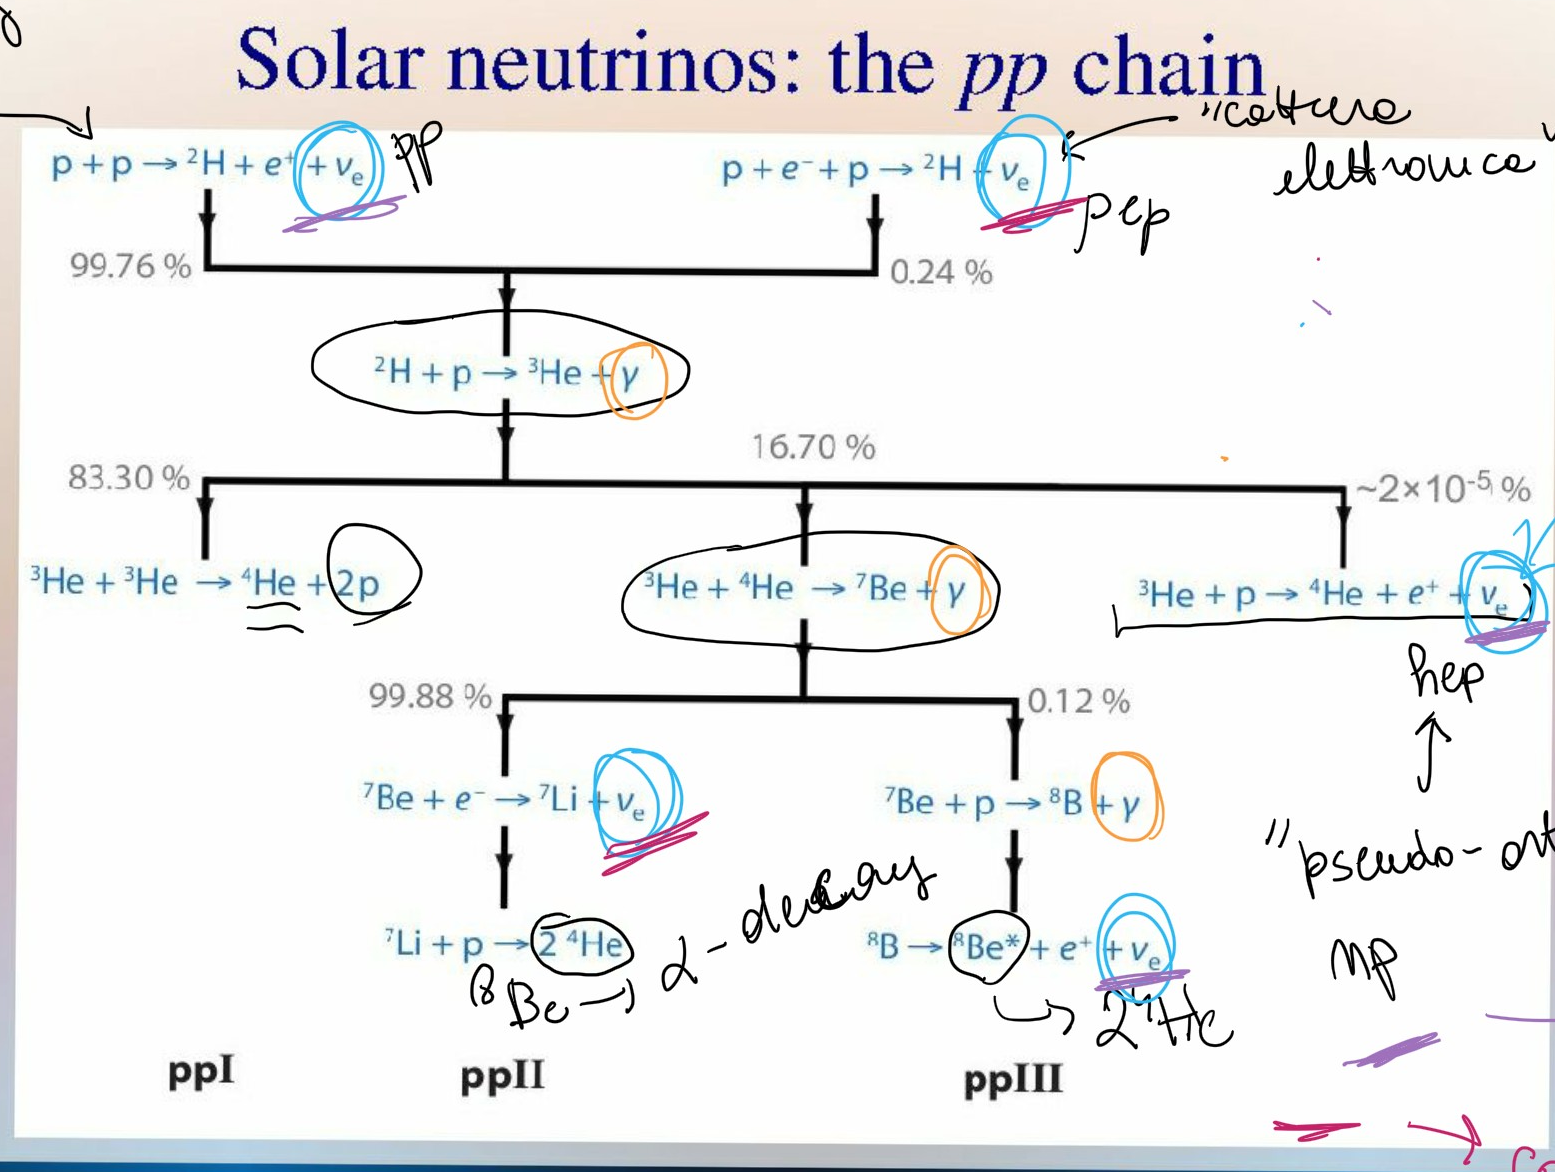
\includegraphics[scale=0.3
    ]{Immagini/0318_solarnu.png}
    \caption{Schema della catena protone-protone. In celeste sono stati cerchiati i neutrini prodotti, di cui quelli sottolineati in viola hanno spettro continuo, mentre quelli sottolineati in magenta hanno spettro a riga. In arancione sono cerchiati i fotoni prodotti. In nero sono cerchiati i decadimenti $\alpha$ del $\ce{^8Be}$.}
    \label{0318_solnu}
\end{figure}

\begin{itemize}
    \item \textbf{Prima reazione:} poiché non esiste uno stato legato per $p+p$ si ha prima un decadimento (tipo $\beta^+$) $p\to n$ e poi $p+n$. Osserviamo che la prima reazione è debole ed è un processo di cattura di 2 protoni\index{Catena protone-protone@Catena protone-protone $pp$!a@$pp$}. Esiste anche la possibilità di un'altra reazione, chiamata $pep$\index{Catena protone-protone@Catena protone-protone $pp$!b@$pep$}, $p+e^-+p$ che assomiglia a una cattura elettronica, ma essendo una reazione a 3 corpi è molto meno probabile della $pp$.
    \item \textbf{Seconda reazione:}\index{Catena protone-protone@Catena protone-protone $pp$!c@$dp$} in questo caso si ha una sola reazione possibile con interazione elettromagnetica, quindi si forma velocemente $\ce{^3He}$.
    \item \textbf{Canale $pp$I:}\index{Catena protone-protone@Catena protone-protone $pp$!e@$pp$I} intuitivamente si sarebbe portati a pensare che la reazione $\ce{^3He} + p$, detta $hep$\index{Catena protone-protone@Catena protone-protone $pp$!d@$hep$}, sia favorita dato che ci sono molti protoni e la barriera coulombiana è la più bassa, anche se è mediata dall'interazione debole; tuttavia questo non accade a causa dell'ortogonalità tra gli stati iniziale e finale (\textit{pseudo-ortogonalità} $np$\index{pseudo-ortogonalità@pseudo-ortogonalità $np$}), rendendo rilevanti i contributi dei termini agli ordini successivi.\\
    Nemmeno $\ce{^3He}+d$ va bene, perché questa ha $A=5$, per cui il primo canale della catena è quello che viene detto catena $pp$I\footnote{Il Sole ha bruciato finora principalmente con questo canale.}, ovvero $\ce{^3He}+\ce{^3He}$.
    \item \textbf{Reazioni successive:} a questo punto si ha una certa abbondanza di $\ce{^4He}$ (prima troppo esigua) e si \vir{sblocca} così la reazione $\ce{^3He}+\ce{^4He}$ (che era presente anche nella BBN\index{Big Bang Nucleosynthesis}) con una probabilità di circa il 17\%. A questo punto ci sono due rami: una cattura o elettronica o radiativa.\\ 
    Il \textbf{canale $pp$II}\index{Catena protone-protone@Catena protone-protone $pp$!f@$pp$II} è mediato dall'interazione debole, tuttavia è più probabile del \textbf{canale $pp$III}\index{Catena protone-protone@Catena protone-protone $pp$!g@$pp$III} che è invece mediato dall'interazione elettromagnetica; ciò è dovuto alla differenza nella barriera di potenziale delle due reazioni.\\
    Infine, per quanto riguarda $\ce{^7Li}+p$ della $pp$II, in realtà questo è un processo in 2 step: $\ce{^7Li}+p\to\ce{^8Be}^*\to2\alpha$, dove l'ultimo decadimento è molto veloce.
\end{itemize} 
Indipendentemente dal ramo della catena si ha sempre la produzione di un $\alpha$ da $4p$.

\paragraph{Evidenze sperimentali} Ovviamente tale modello necessita di una verifica osservabile. I fotoni confermano la luminosità, ma non dimostrano la necessità della nucleosintesi; sono quindi i neutrini (il cui cammino libero nel Sole è maggiore delle sue dimensioni) le principali evidenze. In particolare, neutrini che derivano da differenti reazioni hanno energie diverse\footnote{I neutrini della $hep$, per esempio, sono i più energetici} e anche distribuzioni diverse\footnote{Quelli che compaiono come uno dei 3 corpi di un prodotto avranno spettro continuo, gli altri avranno una riga.}. 


    %   18/03
%%  Il problema dei \nu Solari
%   Reaction rate
%\part*{Lezione 22/03/2021}
\begin{figure}[h]
    \centering
    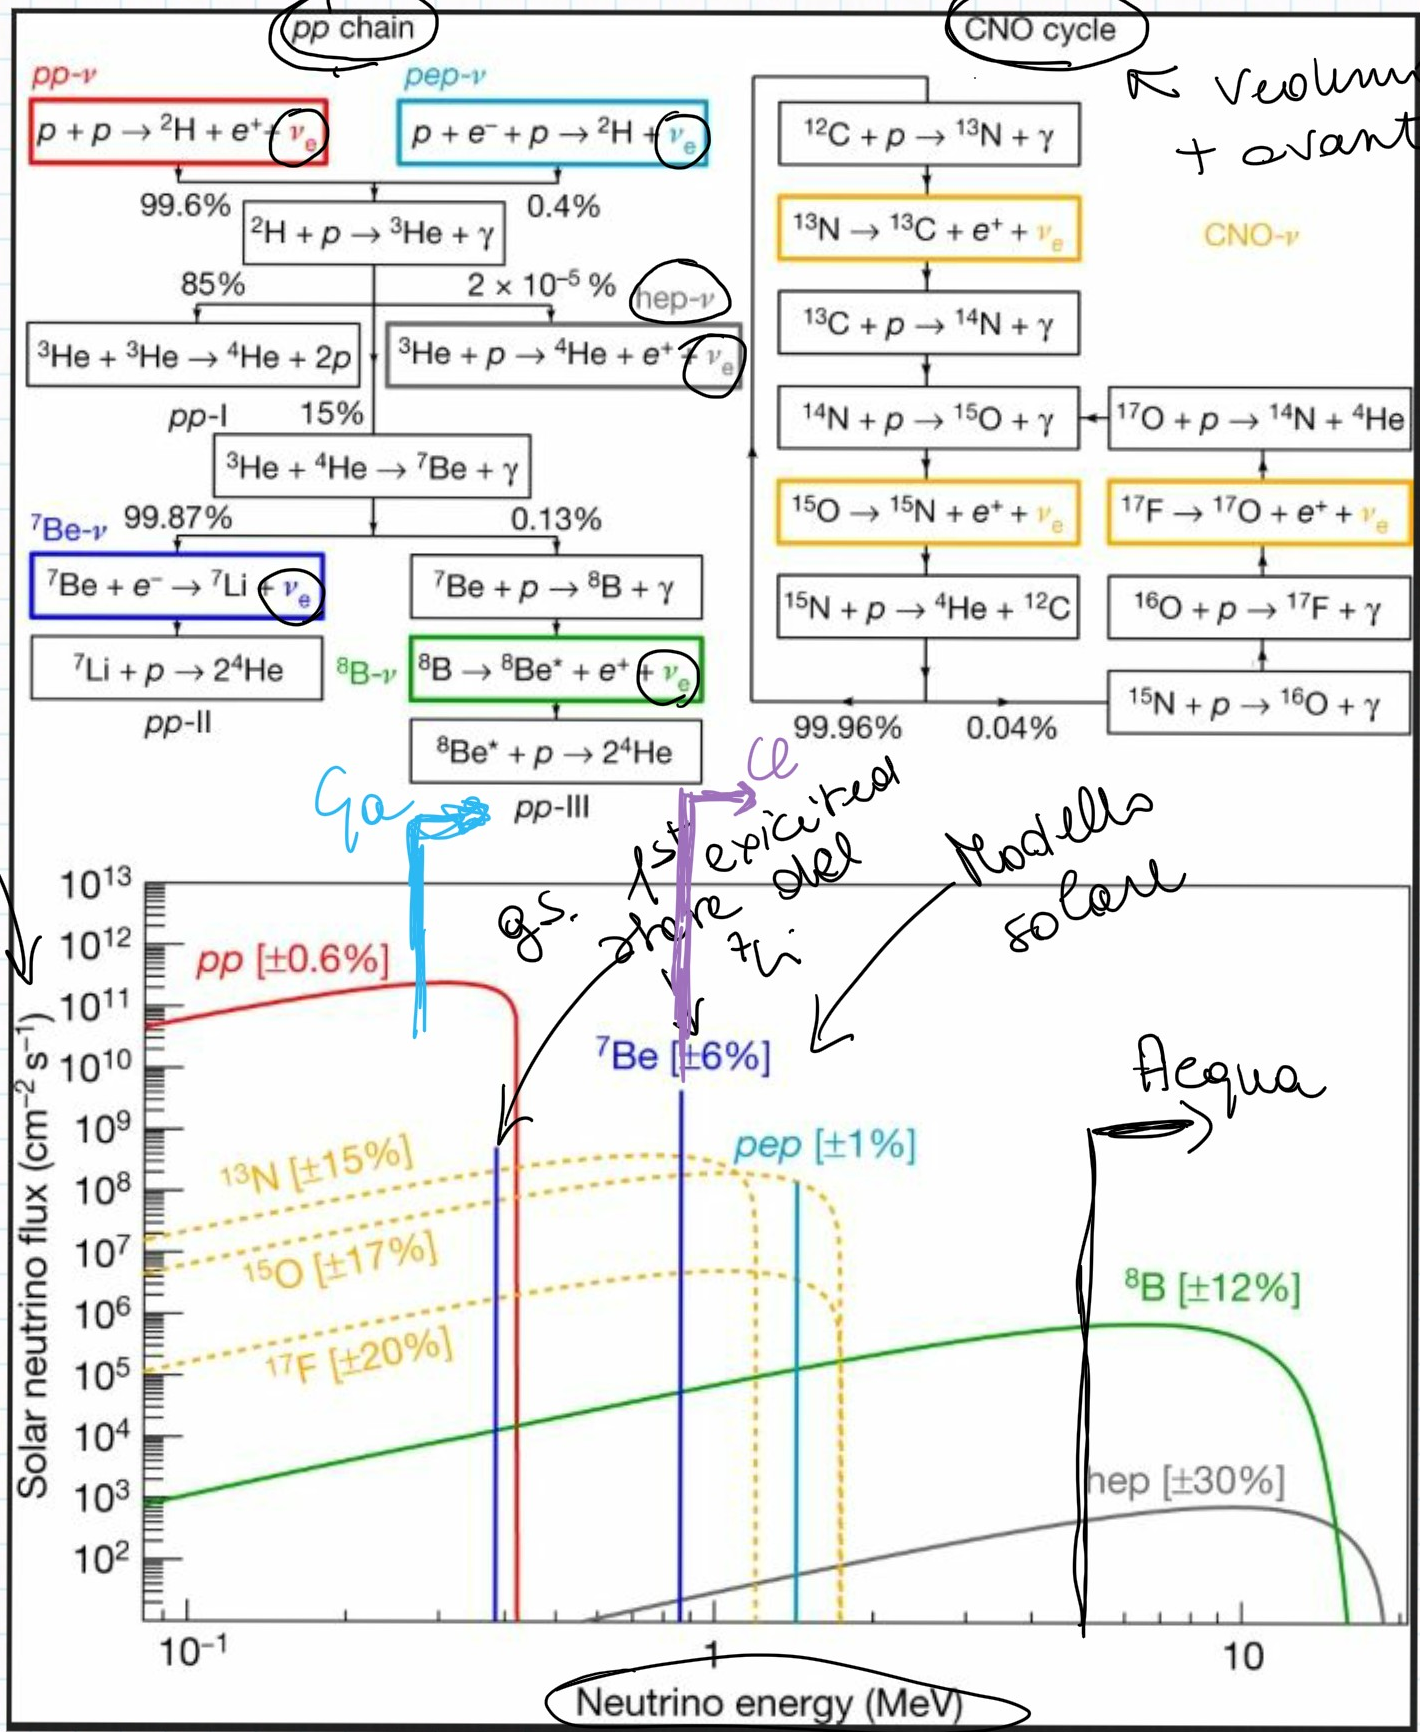
\includegraphics[scale=0.2]{Immagini/0322_neutrini.png}
    \caption[I due processi di produzione dell'elio nel Sole: la catena $pp$ e il biciclo CN-NO. Sotto sono riportati risultati teorici per il vari flussi di neutrini in funzione della loro energia in base alla reazione che li ha prodotti: i rossi, i verdi e i grigi sono uno spettro continuo e il massimo dipende dal fatto che il neutrino è uno di tre corpi; i blu e il turchese sono righe. Ogni flusso ha ovviamente una certa incertezza teorica. La linea viola indica la soglia per l'esperimento di Davis, quella celeste per l'esperimento con il gallio e quella nera per esperimenti con l'acqua. I neutrini del CN-NO hanno tutti uno spettro continuo e sono indicati in giallo.]{I due processi di produzione dell'elio nel Sole: la catena $pp$\index{Catena protone-protone@Catena protone-protone $pp$} e il biciclo CN-NO\index{Ciclo CNNO@Ciclo CN-NO}\footnotemark. Sotto sono riportati risultati teorici per il vari flussi di neutrini in funzione della loro energia in base alla reazione che li ha prodotti: i rossi, i verdi e i grigi sono uno spettro continuo e il massimo dipende dal fatto che il neutrino è uno di tre corpi; i blu e il turchese sono righe. Ogni flusso ha ovviamente una certa incertezza teorica. La linea viola indica la soglia per l'esperimento di Davis, quella celeste per l'esperimento con il gallio e quella nera per esperimenti con l'acqua. I neutrini del CN-NO hanno tutti uno spettro continuo e sono indicati in giallo.}
    \label{0322_nu}
\end{figure}
\footnotetext{Si veda la sezione \secrif{sec-CNNO}.}
\section{Il problema dei neutrini solari}\label{0322-sec-nu}
Come anticipato precedentemente, i neutrini sono i miglior candidati per la verifica sperimentale della nucleosintesi; il primo esperimento di verifica fu fatto da Richard Davis\esperimento{esperimento di Davis} nel 1960 e gli valse il premio Nobel: egli ebbe l'idea di studiare in una miniera del Sud Dakota (detta \textit{Homestake}) la reazione
$$\ce{^{37}Cl} + \nu_e \to \ce{^{37}Ar} + e^-$$
poiché attraverso analisi chimica è possibile contare Ar estratto ed essendo nel sottosuolo l'effetto dei raggi cosmici è attenuato; tuttavia, è necessario avere Cl purissimo. L'esperimento funzionò, i neutrini furono osservati, ma dal momento che la reazione ha una certa energia di soglia ($E_{th}\sim 1$ MeV) perché avvenga gli unici neutrini visibili furono quelli della $pep$, del $\ce{^8B}$ e della $hep$ che come mostrato in Figura \ref{0322_nu} sono i meno numerosi. Il problema principale, però, fu il fatto che il numero di neutrini osservati era circa la metà di quelli previsti.\\
Inizialmente si imputò questa discrepanza alla natura dell'esperimento per cui ne seguirono altri con reazioni differenti, uno di questi fu fatto con il gallio\esperimento{esperimento con il gallio} tra il 1991  il 1997 nel Gransasso:
$$\ce{^{71}Ga + \nu_e \to \ce{^{71}Ge}} +e^-$$
in questo caso l'energia di soglia è $E_{th}\simeq 233.2$ keV (la linea celeste in Figura \ref{0322_nu}), quindi vedo molti più neutrini. Il $\ce{^{71}Ge}$ si estrae attraverso la molecola di $^{71}GeH_4$ e dato che il tempo di dimezzamento del $\ce{^{71}Ge}$ è di circa $11.43$ giorni i neutrini vengono contati dal numero di decadimenti che si osservano. Nonostante i cambiamenti fatti all'apparato sperimentale, il risultato fu la stessa discrepanza. Furono condotti allora esperimenti con rivelatori \cherenkov ad acqua\esperimento{esperimento con acqua}:
$$\nu_e + e^- \to \nu_e + e^- \quad \text{Riculo} \to \text{luce \cherenkov}$$
Il vantaggio della luce \cherenkov è che è direzionale quindi era possibile determinare con precisione se i neutrini venissero dal Sole; lo svantaggio è che oltre ad avere bisogno di molta acqua purissima gli eventi sono pochi, perché l'elettrone per emettere deve superare una certa soglia e questo impone che il neutrino abbia energia alta (la soglia nera in Figura \ref{0322_nu}), per cui si osservano solo quelli del $\ce{^8B}$ e della $hep$. Inoltre, ogni tipo di neutrino può fare tale scattering: i $\nu_\tau$ e i $\nu_\mu$ per esempio possono scambiare solo un bosone che sia neutro, quindi, $Z^0$, mentre i $\nu_e$ oltre a $Z^0$ dato che $\nu_e\to e^-$ o $e^-\to \nu_e$ possono mediare l'interazione anche tramite i bosoni $W^\pm$. In generale non c'è modo di distinguere un processo dall'altro, ma dal momento che $m_W\ll m_Z$ questa interazione è molto più probabile (quindi $\nu_e$ in maggior numero).
\begin{figure}[h]
    \centering
    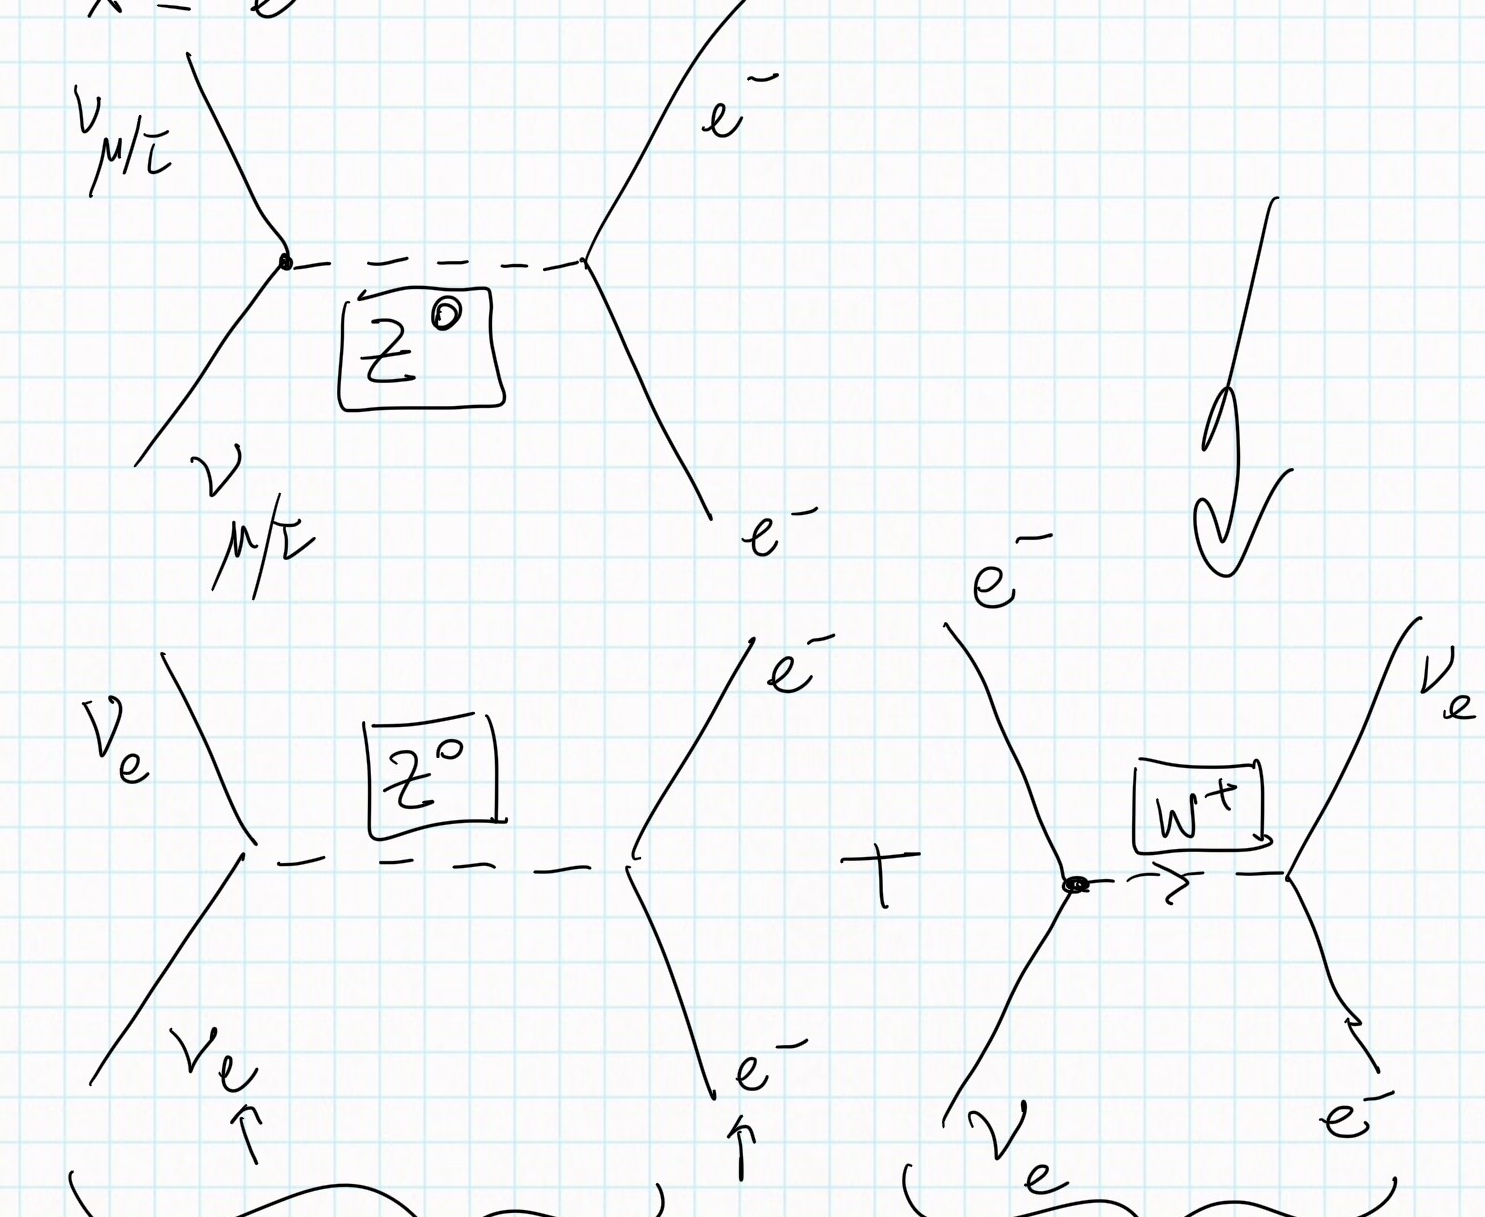
\includegraphics[scale=0.2]{Immagini/0322_Scambio.png}
    \caption{Rappresentazione schematica dell'interazione nello scattering.}
    \label{0322_scambio}
\end{figure}
\noindent Passiamo ora alla descrizione\footnote{Le immagini e i dati sono raccolti nelle \textit{slide} \texttt{Neutrino\_flux\_exp.pdf}.} di 3 esperimenti di questo tipo:
\begin{itemize}
    \item \textbf{Super-Kamiokande} (SK)\esperimento{Super-Kamiokande}: dal nome della miniera Kamioka in Giappone nella quale è situato è il successore del precedente Kamiokande. Contiene una cisterna di $50,000$ tonnellate di acqua costellata di fotomoltiplicatori (maggiormente sensibili ai $\nu_e$) che ne coprono l'intera superficie (circa $11,200$). \\
    Potendo acquisire risultati sia di giorno che di notte, SK osservò una differenza nel numero di neutrini osservati nei due momenti del giorno, in particolare $\#\nu_{notte}<\#\nu_{diurno}$. Per la prima volta però si riesce a dare una spiegazione di queste fluttuazioni: assumendo, infatti, che $m_\nu\not = 0$ si può dimostrare che lo stato di neutrino di interazione debole (quindi di un certo \textit{sapore}) può essere descritto come sovrapposizione di due stati di massa differente %secondo un certo operatore di massa
    , ovvero:
    \begin{displaymath}
    \begin{aligned}
    \st{\nu_e} &= \alpha\, \st{\nu_1} + \beta\, \st{\nu_2}\\
    \st{\nu_\mu} &= \alpha'\, \st{\nu_1} + \beta'\, \st{\nu_2}
    \end{aligned}
    \end{displaymath}
    Lo stato del neutrino di interazione quindi oscilla\index{oscillazione di sapore dei neutrini} $\st{\nu_e}\simeq k \st{\nu_\mu}$ con una probabilità che dipende dalla distanza percorsa prima dell'osservazione e questo spiega la discrepanza con il numero di neutrini previsti dalla teoria. Tuttavia, SK non poté verificarlo perché nel 2001\index{incidente al Super-Kamiokande} durante la manutenzione per la quale viene svuotata la cisterna non si accorsero che un fotomoltiplicatore si era leggermente incrinato e al successivo riempimento, quando il livello era circa a metà, questo fotomoltiplicatore si è rotto; il vuoto al suo interno ha risucchiato l'acqua producendo un'onda d'urto che ha innescato una reazione a catena e ha causando la rottura di 500 fotomoltiplicatori.\\
    Dopo l'incidente i giapponesi iniziarono repentinamente le riparazioni, ma ormai era stato già avviato un altro esperimento in Canada per la verifica della teoria.
    \item \textbf{Sudbury Neutrino Observatory} (SNO)\esperimento{Sudbury Neutrino Observatory}: esperimento con rivelatore \cherenkov situato nella miniera Creighton in Canada, sfruttò l'acqua pesante $\ce{^2H_2O}$ invece della semplice $H_2O$, questo perché oltre allo scattering elastico era possibile anche la reazione\footnote{Si tratta di una $pep$ \vir{al contrario}} $\nu_e + \ce{^2H} \to p+e^-+p$; questa può avvenire solo con $\nu_e$ e si distingue da quella dello scattering dalla luce \cherenkov prodotta. Si noti, però, che è anche possibile:
    $\nu + \ce{^2H} \to \nu + p +n$ ovvero scattering elastico. Per tenerne traccia, furono messe delle impurità di $\ce{^{35}Cl}$ così che $\ce{^{35}Cl}+n\to \ce{^{36}Cl +\gamma}$, identificabile quindi dai fotoni prodotti. Fu allora possibile contare sia il numero di neutrini elettronici che quello di neutrini generici e si ottenne l'evidenza di accordo con il valore predetto dalla teoria: non era quindi il modello solare a dover essere rivisto, ma quello standard.
    \item \textbf{Borexino}\esperimento{Borexino}: in ultima battuta diamo uno sguardo anche al contributo italiano nell'ambito di tale ricerca. In quel periodo infatti al Gransasso era stato sistemato un esperimento che si componeva di uno scintillatore\index{scintillatore} in una camera circondata da fotomoltiplicatori. Il vantaggio era quello di avere una soglia per la reazione molto bassa e questo permise a Boxerino di verificare che nel Sole erano presenti anche le reazioni $pp$, $\ce{^7Be}$ e $pep$, come mostrato in Figura \ref{0322_risultati}.\\
    \noindent Una piccola nota dolente: Boxerino sarebbe stato capace di verificare l'oscillazione dei neutrini prima dell'esperimento canadese, tuttavia la burocrazia italiana ha ritardato enormemente l'arrivo dei fondi.
    \begin{figure}[ph]
        \centering
        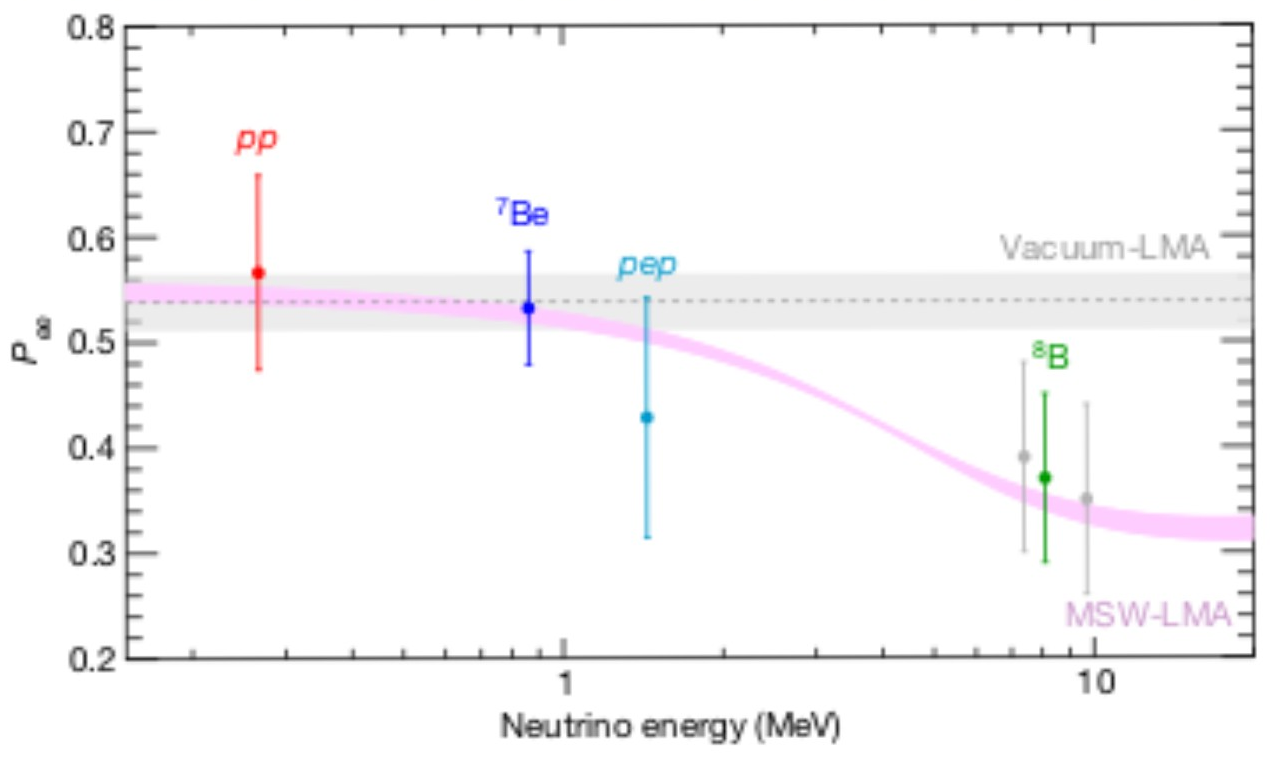
\includegraphics[scale=0.2]{Immagini/0322_energianu.png}
        \caption{Probabilità di sopravvivenza del neutrino in funzione della sua energia. I punti sono i risultati ottenuti da Boxerino, in rosa la predizione teorica e in grigio il modello con parametri di oscillazione dati dai risultati di SNO.}
        \label{0322_risultati}
    \end{figure}
    \begin{figure}[p!h]
        \centering
        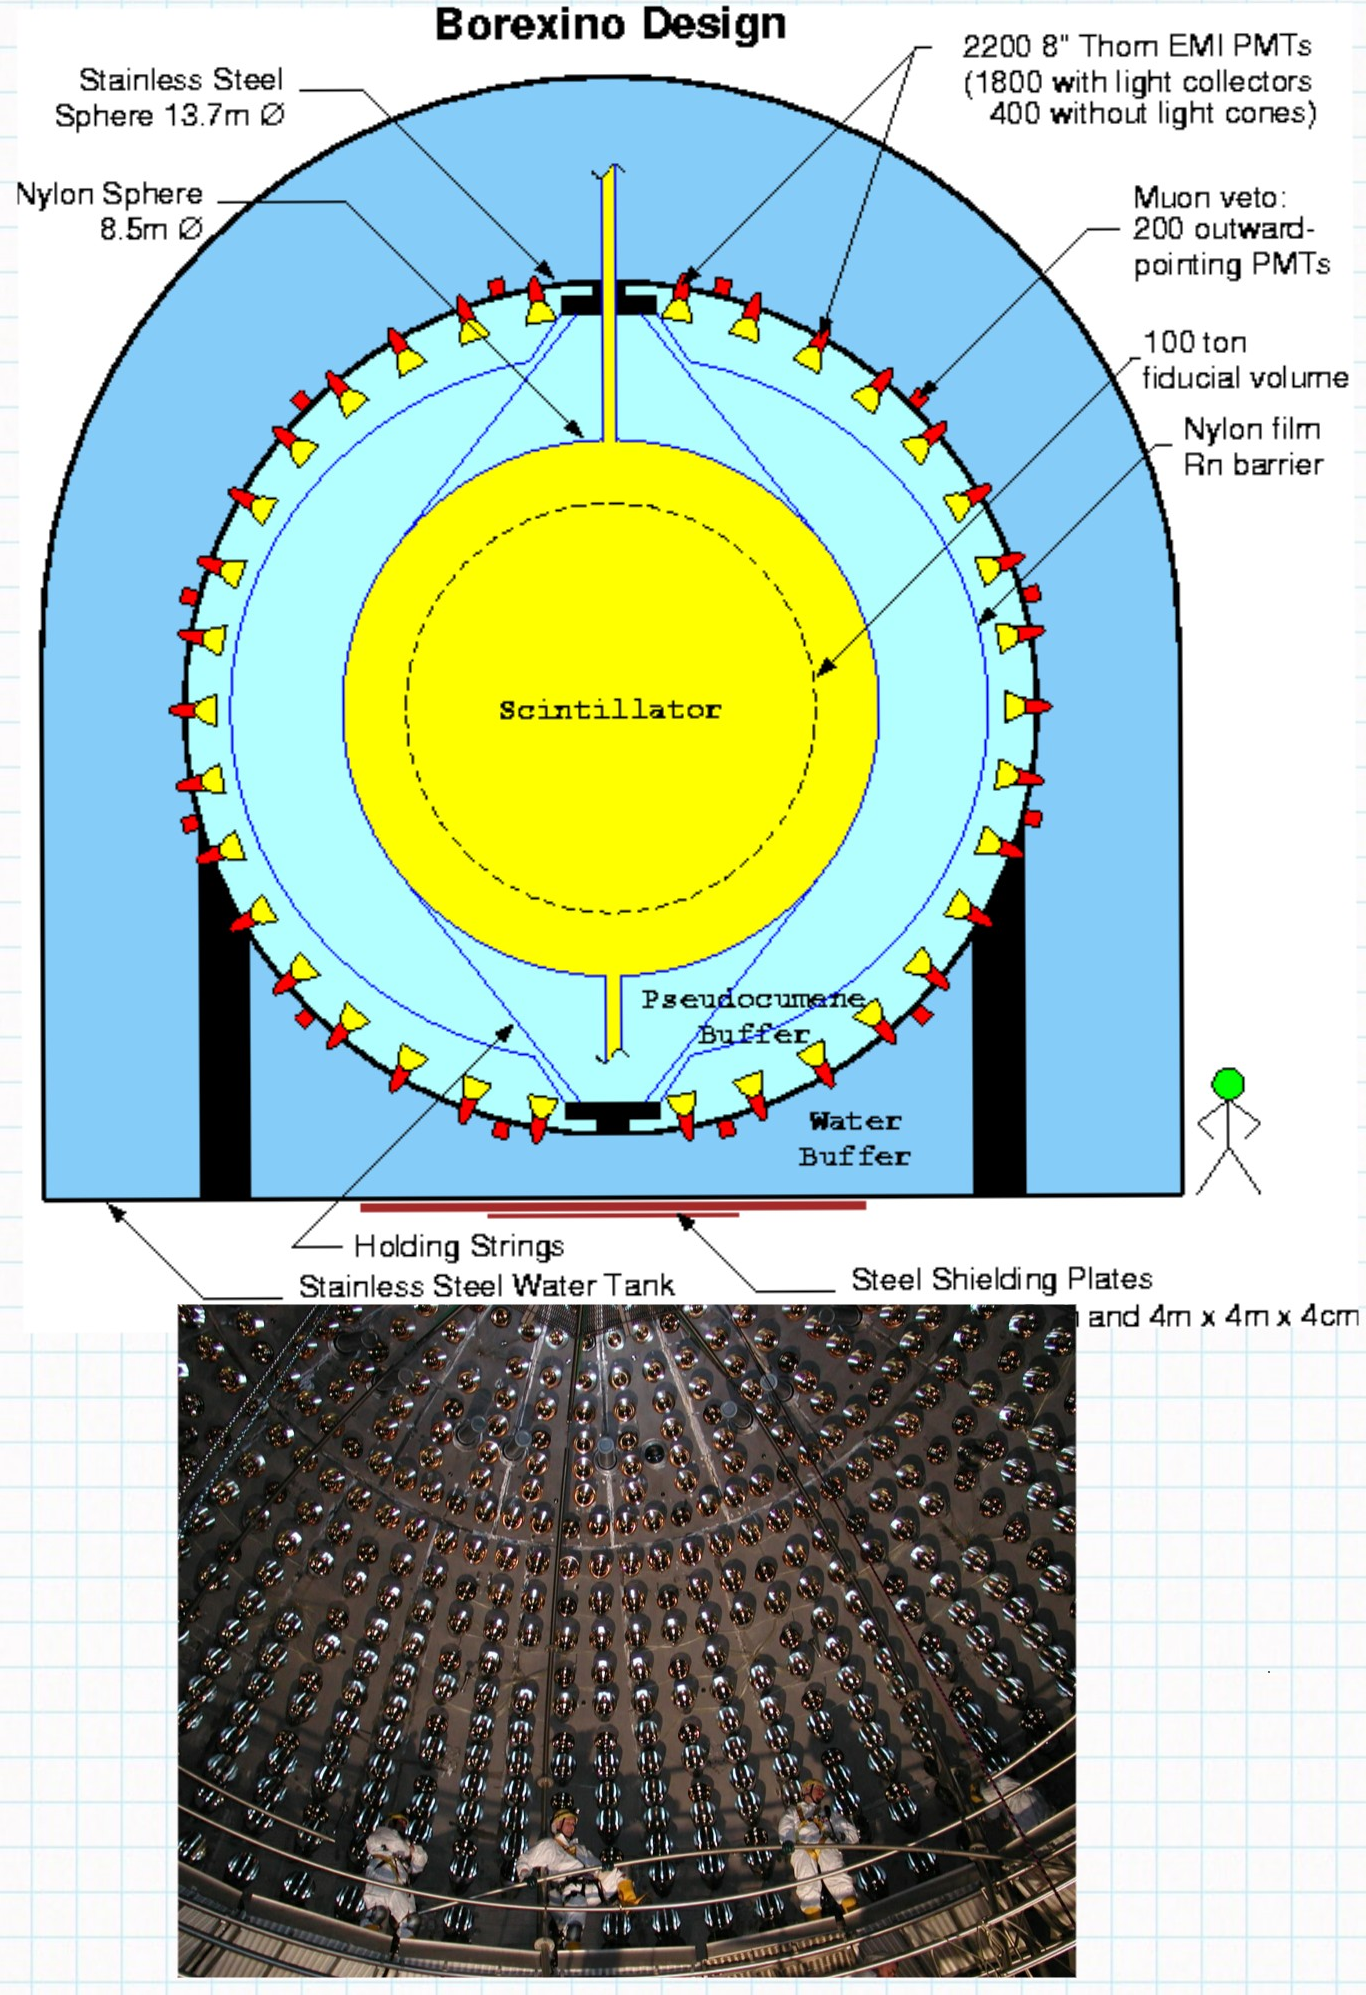
\includegraphics[scale=0.2]{Immagini/0322_borexino.png}
        \caption{Schema e foto dell'esperimento Boxerino.}
        \label{0322_box}
    \end{figure}
\end{itemize}

\newpage

\section{Elementi di calcolo}
Introduciamo adesso alcuni elementi essenziali per l'analisi nucleare, che utilizzeremo successivamente nello studio della catena $pp$.

\subsection{Fattore Astrofisico}
Consideriamo una generica reazione con particelle (proiettili) che incidono su nuclei (bersagli):
$$a+X\to b+Y$$
Dall'analisi dimensionale abbiamo per la sezione d'urto:
$$\sigma[L^2] = \frac{\# \text{reazioni}/\text{nucleo X}/\text{unità di tempo}}{\underbrace{\# \text{proiettili}/L^2/\text{unità di tempo}}_\text{flusso particelle incidenti}}$$
%\footnote{Nell'espressione abbiamo chiamato \textit{rate} il numeratore; in realtà, il \textit{rate} è in unità di volume e non di nucleo $X$.}
Cerchiamo di costruire l'espressione per il \textit{reaction-rate} $r$\index{reaction-rate@\textit{reaction-rate} $r$}: se $N_a$ è la densità numerica dei proiettili, $\vec{v}$ la loro velocità di volo e $N_X$ la densità numerica dei bersagli allora si ha $r = N_a N_X\, \sigma v$; in generale però potremmo avere $a=X$ e non potendo distinguere tra i due con l'espressione precedente si otterrebbe il doppio del \textit{rate} effettivo, per cui: 
$$r = \frac{N_a N_X}{1+\delta_{aX}}\: \mean{\sigma(\vec{v})\, v}$$
dove abbiamo mediato sulla distribuzione in velocità, che nel caso stellare è una Maxwelliana $\phi(v)$, poiché in generale non tutti i proiettili avranno velocità $\vec{v}$. Procedendo con il calcolo:
\begin{displaymath}
\begin{aligned}
\mean{\sigma(\vec{v})\, v} &= \int_0^\infty \sigma \, v \: \phi(v) dv = \\
&= \int_0^\infty \sigma \, v \: 4\pi \ppc{\frac{\mu}{2\pi kT}}^{3/2} \exp{\ppc{-\frac{\mu v^2}{2kT}}} v^2 dv = \qquad \text{sostituendo } E= \frac{1}{2}\mu v^2\\
&= 4\pi \ppc{\frac{\mu}{2\pi kT}}^{3/2} \int_0^\infty \frac{1}{\mu^2} 2E\, \sigma(E) \, e^{-E/kT} \: dE =\\
&= \sqrt{\frac{8}{\pi \mu}} \ppc{\frac{1}{kT}}^{3/2} \, \int_0^\infty \sigma(E) \, e^{-E/kT} \: dE
\end{aligned}
\end{displaymath}
La dipendenza di $\sigma$ da $E$ dipende principalmente da tre fattori:
\begin{enumerate}
    \item La probabilità di attraversamento della barriera Coulombiana.
    \item La probabilità di avere un'interazione.
    \item La prossimità a una risonanza nucleare.\index{risonanza nucleare}
\end{enumerate}
Tutti e tre infatti dipendono dall'energia. Studiamo prima le reazioni non-risonanti: per il secondo dalla meccanica quantistica sappiamo che la probabilità di interazione è proporzionale a\footnote{$\pi\lambda_{DB}^2$ non è altro che la sezione d'urto.} $\pi \lambda^2_{DB}\sim p^{-2} \sim E^{-1}$\index{lunghezza d'onda di De Broglie@lunghezza d'onda di De Broglie $\lambda_{DB}$}; per il primo l'espressione è un po' più complessa, ma nel Sole ho tutte particelle cariche quindi:
$$V = \frac{Z_1 Z_2 e^2}{r} \simeq 1.44 \, \frac{Z_1Z_2}{r[\mbox{fm}]} [\mbox{MeV}] \underset{\text{per }pp}{\sim} 1.44\unit{MeV}$$
L'energia di agitazione termica media $\mean{E}\sim kT \sim 9\cdot\ord{-8} \, T[\mbox{K}]\,[\mbox{keV}]$ per la temperatura interna del Sole ($T\sim 1.5\cdot\ord{7}$ K) è dell'ordine del keV, quindi trascurabile rispetto alla barriera. Valutiamo allora la probabilità di attraversamento per effetto tunnel\index{effetto tunnel}:
\begin{displaymath}
\begin{aligned}
P &\sim \exp{\PPc{-2\pi \frac{Z_1Z_2 e^2}{\hbar v}}} =\\
&= \exp{\PPc{-2\pi \frac{Z_1Z_2 e^2}{\hbar}\, \sqrt{\frac{\mu}{E}}}} =\\
&= \exp{\PPc{-\sqrt{2\mu}\pi\, \frac{Z_1Z_2 e^2}{\hbar \sqrt{E}}}} 
\end{aligned}
\end{displaymath}
detto \textbf{fattore di penetrazione di Gamow}\index{fattore di penetrazione di Gamow}. Per quanto riguarda i vari contributi nucleari possiamo raccoglierli tutti in un fattore $S(E)$ che chiamiamo \textbf{fattore astrofisico}\index{fattore astrofisico@fattore astrofisico $S(E)$}; abbiamo allora:
$$\sigma (E) = \frac{1}{E}\,\exp{\PPc{-\sqrt{2\mu}\pi\, \frac{Z_1Z_2 e^2}{\hbar \sqrt{E}}}}\, S(E)$$
\noindent A titolo di esempio riportiamo l'andamento di $\sigma(E)$ per la reazione $\ce{^{12}C}+p\to \ce{^{13}N}+\gamma$ in Figura \ref{0322_cross}. Si osserva una risonanza per circa mezzo MeV e che la sezione precipita sotto 0.3 MeV (è dovuto al fattore di Gamow); in rosso è segnato il range di energie di interesse astrofisico.
\begin{figure}[!h]
    \centering
    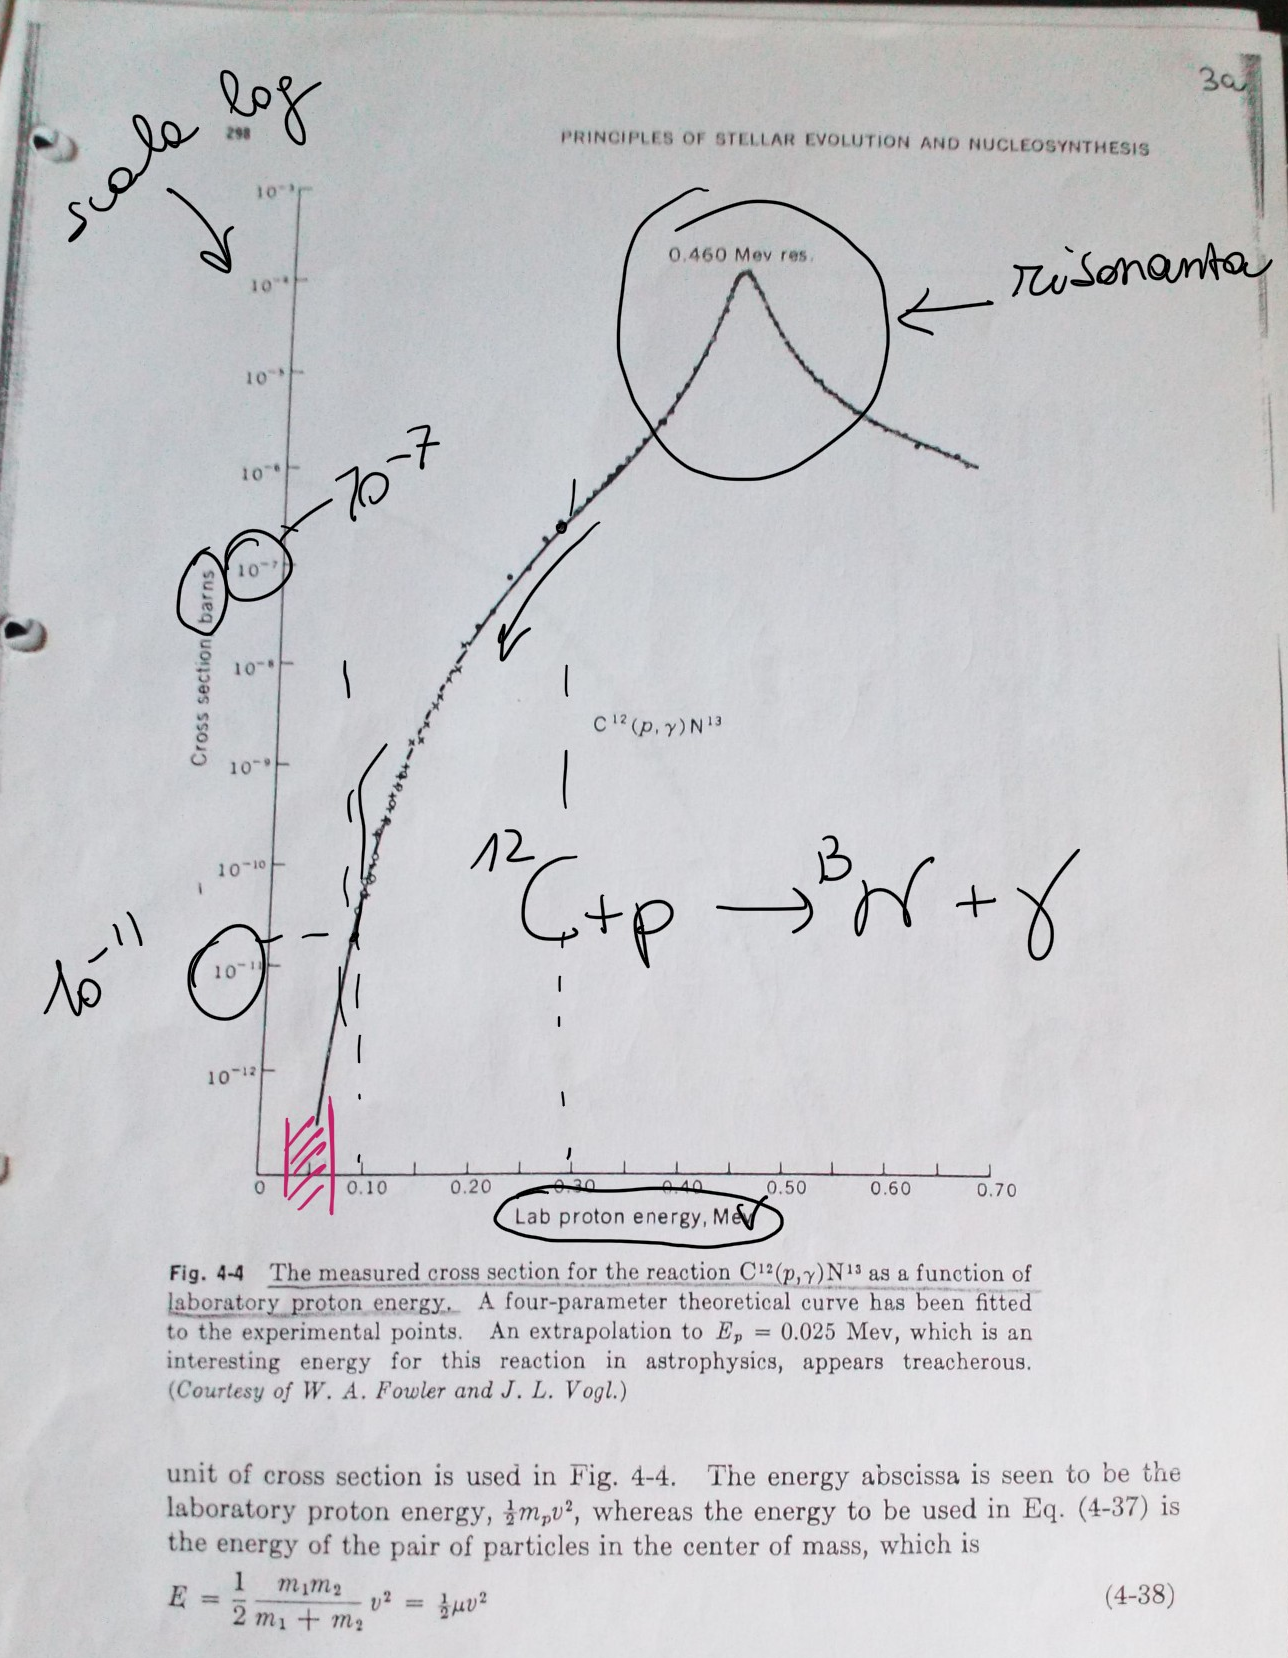
\includegraphics[scale=0.2]{Immagini/0322_crosssection.png}
    \caption{Leggere la didascalia. In rosso il range di energie di interesse astrofisico.}
    \label{0322_cross}
\end{figure}\\
\noindent Dall'espressione per la sezione d'urto possiamo invertire per ottenere l'andamento del fattore astrofisico $S(E) = E \sigma(E)\exp(\dots)$ come mostrato in Figura \ref{0322_fatastr}. Si nota che in questo caso la pendenza per basse energie è più \vir{dolce} (maggior stabilità).

\begin{figure}[h]
    \centering
    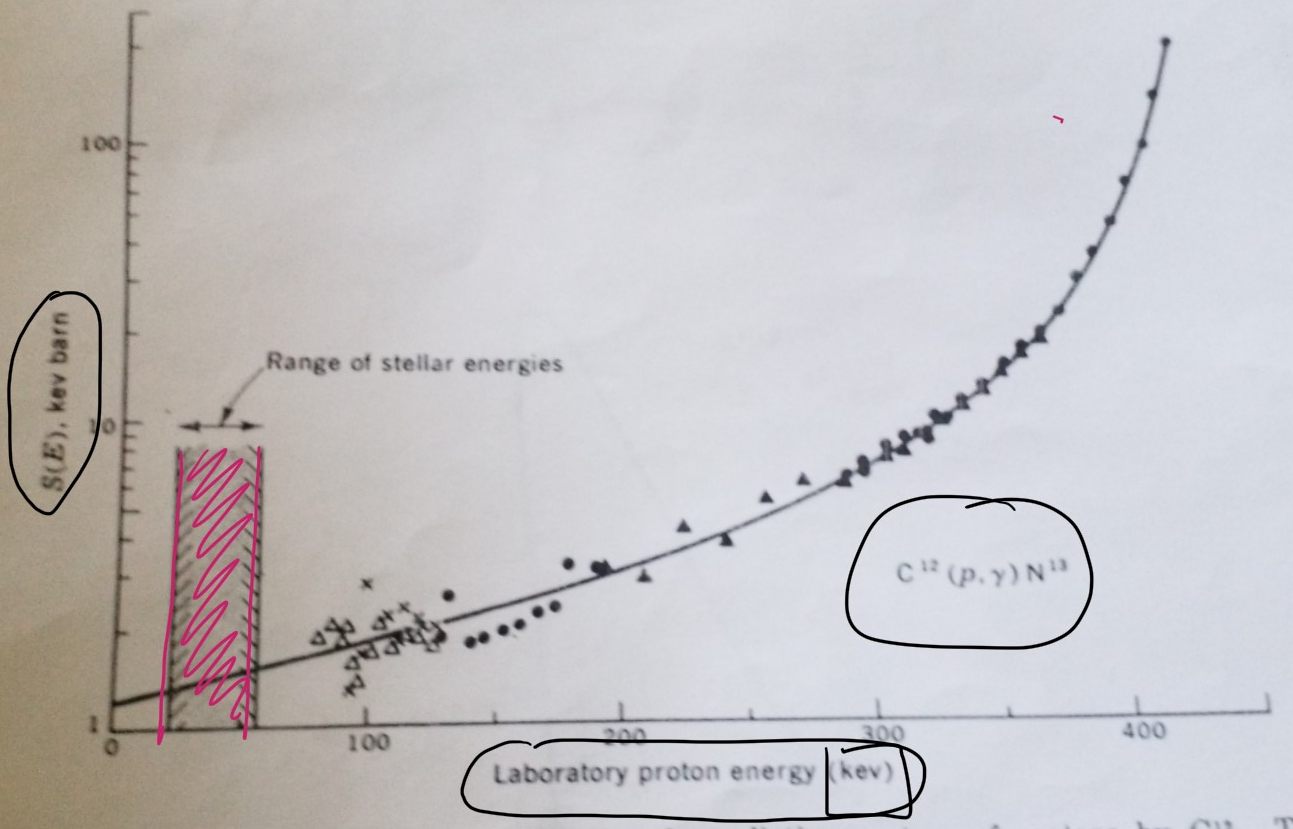
\includegraphics[scale=0.3]{Immagini/0322_fattoreastr.png}
    \caption{Andamento del fattore astrofisico per la reazione precedente.}
    \label{0322_fatastr}
\end{figure}
    %   22/03
%%  Fine Reaction rate
%   Fattore astrofisico
%\part*{Lezione 24/03/2021}
%\noindent Riprendiamo dall'espressione ottenuta precedentemente per $\sigma$:
%$$\sigma (E) = \frac{1}{E}\,\exp{\PPc{-\sqrt{2\mu}\pi\, \frac{Z_1Z_2 e^2}{\hbar \sqrt{E}}}}\, S(E)$$
\paragraph{Fattore astrofisico} 
Sostituiamo l'espressione per la sezione d'urto nel calcolo del \textit{reaction-rate}:
\begin{displaymath}
\begin{aligned}
\mean{\sigma\, v } &= \sqrt{\frac{8}{\pi\mu}} \ppc{\frac{1}{kT}}^{3/2} \int_0^\infty \frac{1}{E}\,\exp{\PPc{-\sqrt{2\mu}\pi\, \frac{Z_1Z_2 e^2}{\hbar \sqrt{E}}}}\, S(E) \; \exp{\ppc{-\frac{E}{kT}}} E dE = \\
&= \sqrt{\frac{8}{\pi\mu}} \ppc{\frac{1}{kT}}^{3/2} \int_0^\infty S(E) \: \exp{(-f(E))} \\
f(E) &\equiv \frac{E}{kT} + \frac{b}{\sqrt{E}}\\
b &\equiv \sqrt{2\mu}\pi\, \frac{Z_1Z_2 e^2}{\hbar} \simeq 0.99 \, Z_1 Z_2 A^{1/2} \unit{MeV}^{1/2}\; \footnotemark 
\end{aligned}
\end{displaymath}
\begin{figure}
    \centering
    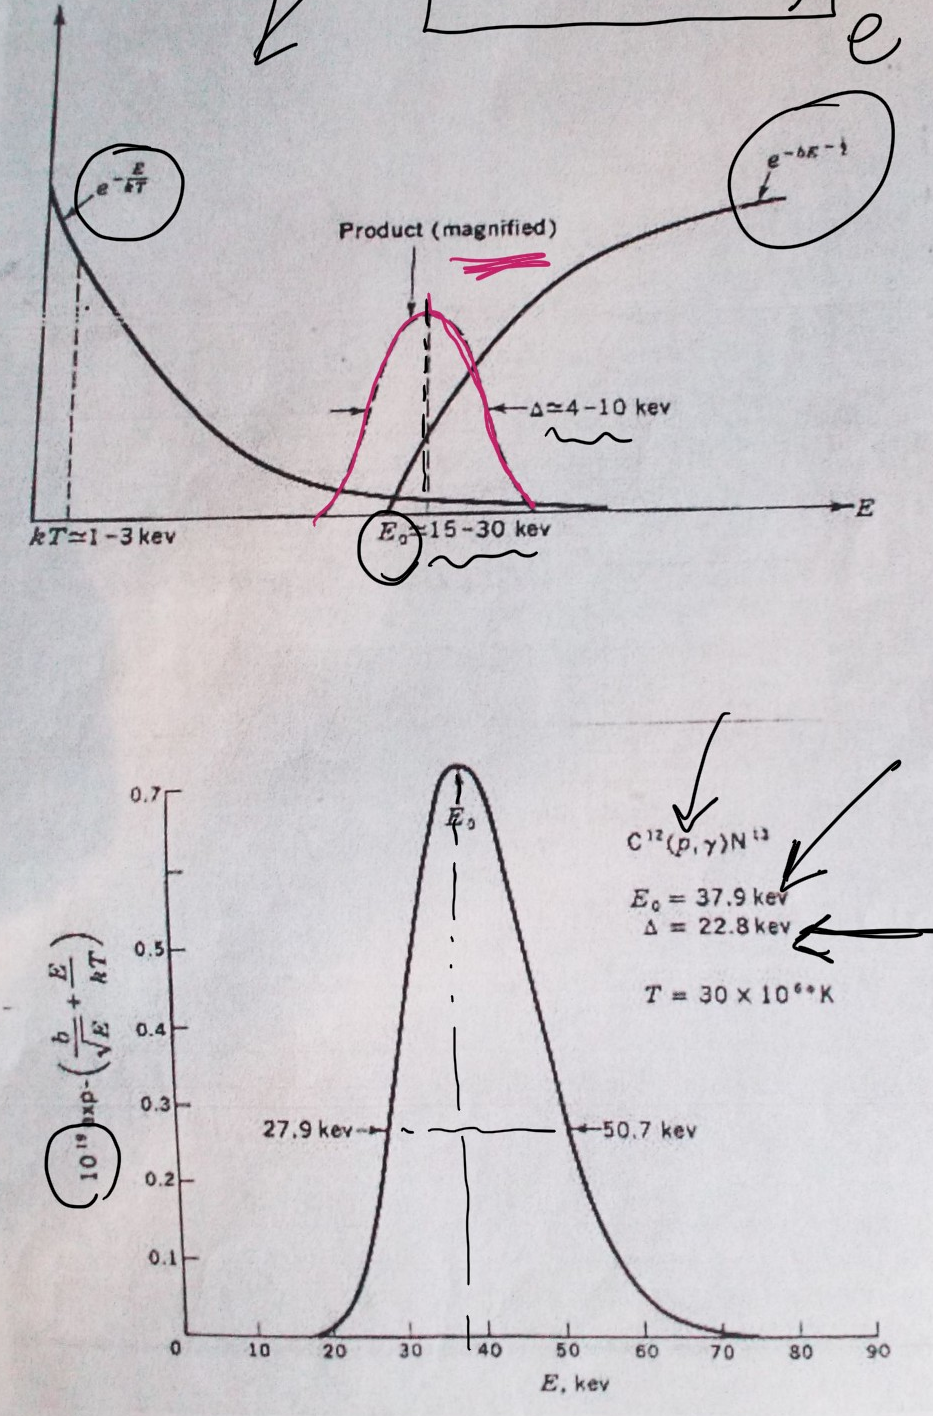
\includegraphics[scale=0.2]{Immagini/0324_gamow2.png}
    \caption{In alto l'andamento di $\exp{(-E/kT)}$, di $\exp{(-b/\sqrt{E})}$ e di $\exp{(-f(E))}$; in basso l'ingrandimento del picco di Gamow\index{picco di Gamow}.}
    \label{0324_picco}
\end{figure}
\footnotetext{Qui $A$ è la massa ridotta in unità di masse atomiche.}
\noindent Studiamo allora l'andamento $\exp{(-f(E))}$ in Figura \ref{0324_picco}. Notiamo che per $E=E_0$ si ha un massimo, per cui $f'(E_0) = 0$ da cui\footnote{Con $T_6$ si intende $T = T_6 \cdot \ord{6}\unit{K}$.}: 
$$E_0 = (\frac{b}{2}kT)^{2/3} \simeq 1.22 \, (Z_1Z_2 A^{1/2} T_6)^{2/3}\unit{keV} $$
questa è l'energia più probabile e $f(E_0)$ è detto \textbf{picco di Gamow}\index{picco di Gamow}. Notiamo che il picco è molto sensibile alla temperatura; per esempio nel Sole ($T_6\simeq 15$) per la $pp$ si ha $E_0 = 1.22\, (15\cdot \sqrt{1/2})^{2/3} = 5.89$ keV. In generale, $E_0$ è un valore caratteristico della stella.\\
Dal momento che non conosciamo $S(E)$ per ogni $E$, cercheremo di sviluppare l'integrale e a tale scopo definiamo $\tau\equiv f(E_0)= 3E_0/kT$\footnote{$f(E_0)$ si calocola facilmente sostituendo $b=2E_0^{2/3}/kT$.} (nel Sole $\tau_{pp}\sim 14\gg 1$) e riscriviamo $f(E)$ come:
\begin{displaymath}
\begin{aligned}
f(E) &= \PPc{\frac{E}{3E_0}\tau + \frac{b}{\sqrt{E}}\frac{kT}{3E_0} \tau} =\\
&= \tau \, \PPc{\frac{E}{3E_0} + \frac{2E_0^{3/2}}{kT \sqrt{E}}\frac{kT}{3E_0}} =\\
&= \tau \, \PPc{\frac{E}{3E_0} + \frac{2}{3}\sqrt{\frac{E_0}{E}}}\\
\text{Definiamo } x \text{ tale che } E&\equiv E_0 \ppc{1+\frac{2x}{\sqrt{\tau}}}\\
E-E_0 &= \frac{2x}{\sqrt{\tau}}E_0 = 2\sqrt{\frac{kTE_0}{3}}\,x \equiv \frac{\Delta}{2} x
\end{aligned}
\end{displaymath}
dove abbiamo definito $\Delta \equiv 4\sqrt{kTE_0/3}$ (per il Sole $\Delta_{pp}\sim 6.4$ keV)%che somiglia molto alla HWFH della Gaussiana
. Facciamo allora un'espansione\footnote{Si ricordi che $f'(E_0)=0$ e che $\tau/2E_0^2 = 8/\Delta^2$, per cui $f(x) = f(E_0) + ((E-E_0)/(\Delta/2))^2 + \dots$.} di $f(E)$ intorno a $E_0$, che in termini di $x$ è un'espansione intorno a $x=0$:
\begin{displaymath}
\begin{aligned}
f(x) &= \tau \, \PPq{\frac{1}{3} \ppc{1+\frac{2x}{\sqrt{\tau}}} + \frac{2}{3} \frac{1}{\sqrt{\ppc{1+2x/\sqrt{\tau}}}}} \simeq\\
&\simeq \PPq{\frac{1}{3} \ppc{1+\frac{2x}{\sqrt{\tau}}} + \frac{2}{3} \PPc{1-\frac{x}{\sqrt{\tau}} +\frac{3}{2}\frac{x^2}{\tau} - \frac{5}{2} \frac{x^3}{\tau\sqrt{\tau}}+\frac{35}{8}\frac{x^4}{\tau^2}+ O(x^5)} } \simeq \\
&\simeq \tau  + x^2 - \frac{5}{3} \frac{x^3}{\sqrt{\tau}} + \frac{35}{12}\frac{x^4}{\tau}
\end{aligned}
\end{displaymath}
Sostituendo allora nell'integrale:
\begin{displaymath}
\begin{aligned}
\int_0^\infty S(E) \exp{(-f(E))}\,dE &\simeq \int_{-\sqrt{\tau}/2}^\infty dx\, S(x) \, \frac{2E_0}{\sqrt{\tau}} \: e^{-\tau} e^{-x^2} \, \underbrace{\exp{\ppc{\frac{5}{3} \frac{x^3}{\sqrt{\tau}} - \frac{35}{12}\frac{x^4}{\tau}}}}_\text{Parte non Gaussiana} \simeq \\
&\simeq  \int_{-\sqrt{\tau}/2}^\infty dx\, S(x) \, \frac{2E_0}{\sqrt{\tau}} \: e^{-\tau} e^{-x^2} \, \ppc{1+\frac{5}{3} \frac{x^3}{\sqrt{\tau}} - \frac{35}{12}\frac{x^4}{\tau} + \frac{25}{18} \frac{x^6}{\tau}}
\end{aligned}
\end{displaymath}
dove al primo passaggio abbiamo cambiato variabile $dE = dx\,2E_0/\sqrt{\tau}$ e successivamente sviluppato l'esponenziale al II ordine, trascurando i termini $O(x^7)$. Per procedere analiticamente con il calcolo sviluppiamo anche il fattore astrofisico\index{fattore astrofisico@fattore astrofisico $S(E)$} intorno a $E_0$: $S(E) = S(E_0) + (2xE_0/\sqrt{\tau})\,S'(E_0) + (2x^2E_0^2/\tau)\,S''(E_0)+\dots$; studiamo l'integrale dei vari ordini\footnote{Useremo principalmente che:
$$\int_{-\infty}^{+\infty} e^{-x^2} x^n = \Bigl \{ %
\begin{array}{ll}
    0 & n=2s+1 \\
    (2s-1)!!\:2^{-s} \: \sqrt{\pi} & n=2s
\end{array}%
$$%
Inoltre dal momento che $\tau$ è \vir{grande} (si guardi l'esempio di $\tau_{pp}$) si approssima nell'estremo dell'integrale $-\sqrt{\tau}\sim-\infty$ e poi si sfrutta la parità della funzione integranda.}:
\begin{displaymath}
\begin{aligned}
\text{Ordine 0}& \\
&S(E_0) \, \frac{2E_0}{\sqrt{\tau}}\,e^{-\tau} \int_{-\sqrt{\tau}/2}^\infty dx \:  e^{-x^2} \, \ppc{1+\frac{5}{3} \frac{x^3}{\sqrt{\tau}} - \frac{35}{12}\frac{x^4}{\tau} + \frac{25}{18} \frac{x^6}{\tau}}\simeq \\
\simeq\: &S(E_0) \, \frac{2E_0}{\sqrt{\tau}}\,e^{-\tau} \: 2\int_{0}^\infty dx \:  e^{-x^2} \, \ppc{1- \frac{35}{12}\frac{x^4}{\tau} + \frac{25}{18} \frac{x^6}{\tau}} = \\
= \:&\frac{2E_0}{\sqrt{\tau}}\,e^{-\tau} \,S(E_0) \,\sqrt{\pi}\; \ppc{1-\frac{5}{12}\frac{1}{\tau}} \\
\text{Ordine 1}& \\
&S'(E_0) \, \frac{4E_0^2}{\tau}\,e^{-\tau} \int_{-\sqrt{\tau}/2}^\infty dx \: x e^{-x^2} \, \ppc{1+\frac{5}{3} \frac{x^3}{\sqrt{\tau}} - \frac{35}{12}\frac{x^4}{\tau} + \frac{25}{18} \frac{x^6}{\tau}}\simeq \\
\simeq \:&S'(E_0) \, \frac{4E_0^2}{\tau}\,e^{-\tau} \:2\int_{0}^\infty dx \: x e^{-x^2} \, \frac{5}{3} \frac{x^3}{\sqrt{\tau}}= \\
=\:&\frac{5E_0^2}{\tau\sqrt{\tau}}\,e^{-\tau} \, S'(E_0) \,\sqrt{\pi} \\
\text{Ordine 2}& \\
&S''(E_0) \, \frac{4E_0^3}{\tau\sqrt{\tau}}\,e^{-\tau} \int_{-\sqrt{\tau}/2}^\infty dx \: x^2 e^{-x^2} \, \ppc{1+\frac{5}{3} \frac{x^3}{\sqrt{\tau}} - \frac{35}{12}\frac{x^4}{\tau} + \frac{25}{18} \frac{x^6}{\tau}}\simeq \\
\simeq\: &S''(E_0) \, \frac{4E_0^3}{\tau\sqrt{\tau}}\,e^{-\tau}\: 2 \int_{0}^\infty dx \: x^2 e^{-x^2} \, \ppc{1 \underbrace{- \frac{35}{12}\frac{x^4}{\tau} + \frac{25}{18} \frac{x^6}{\tau}}_{O(1/\tau^2)}}\simeq \\
\simeq \:&\frac{2E_0^3}{\tau\sqrt{\tau}}\,e^{-\tau}\,S''(E_0) \,\sqrt{\pi}
\end{aligned}
\end{displaymath}
Troviamo così per il \textit{reaction-rate}\index{reaction-rate@\textit{reaction-rate} $r$}:
\begin{displaymath}
\begin{aligned}
\mean{\sigma\,v } &=  \sqrt{\frac{8}{\pi\mu}} \ppc{\frac{1}{kT}}^{3/2} \frac{2E_0}{\sqrt{\tau}}e^{-\tau}\sqrt{\pi}\: \underbrace{ S(E_0) \PPq{1+\frac{1}{\tau} \PPc{\frac{5}{12} +\frac{5}{2} \frac{S'(E_0)}{S(E_0)}E_0 + \frac{S''(E_0)}{S(E_0)}E_0^2}} } \equiv\\
&\equiv \sqrt{\frac{8}{\pi\mu}} \ppc{\frac{1}{kT}}^{3/2} \frac{2E_0}{\sqrt{\tau}}e^{-\tau}\sqrt{\pi}\; S_{eff} =\\
&= \frac{2^{7/2}}{3^{5/2}} \frac{\tau^2 e^{-\tau}}{b\sqrt{\mu}}\, S_{eff} \equiv\\
&\equiv K \frac{1}{AZ_1Z_2} \tau^2 e^{-\tau} \: S_{eff}
\end{aligned}
\end{displaymath}
dove abbiamo usato il fatto che\footnote{Si ricavano direttamente dalle definizioni di $b$ e di $\tau$.} $E_0 = (bkT/2)^{2/3}$ e $kT = 27\,b^2/4\tau^3$ e abbiamo definito il fattore astrofisico efficace $S_{eff}$\index{fattore astrofisico@fattore astrofisico $S(E)$!efficace@efficace $S_{eff}$} e la costante $K\simeq 7.2\cdot\ord{-19}$. Osserviamo che $\mean{\sigma\,v}$ dipende fortemente da $\tau$, ovvero dalla struttura della stella tramite $T$, e lo stesso vale per $S_{eff}$; per quanto riguarda quest'ultimo, facciamo uno sviluppo del fattore astrofisico e delle sue derivate in un intorno di $E=0$ fino all'ordine 2 in $S$\footnote{Per cui:%
\begin{displaymath}%
\begin{aligned}%
&S(E_0)   \simeq S(0) + S'(0) E_0 + \frac{1}{2} S''(0) E_0^2 \\ 
&S'(E_0)  \simeq  S'(0)  + S''(0) E_0 \\ 
&S''(E_0) \simeq  S''(0)
\end{aligned}%
\end{displaymath}%
}:
\begin{displaymath}
\begin{aligned}
S_{eff} &\simeq S(0)\, \ppc{1+\frac{5}{36}\frac{kT}{E_0}} +\\
&+ S'(0) E_0\, \ppc{1+\frac{35}{36}\frac{kT}{E_0}} +\\
&+ S''(0) E_0^2\, \frac{1}{2} \ppc{1+\frac{89}{36}\frac{kT}{E_0}}
\end{aligned}
\end{displaymath}
Questa espressione permette di trovare $S_{eff}$\index{fattore astrofisico@fattore astrofisico $S(E)$!efficace@efficace $S_{eff}$} indipendentemente dalla stella presa in considerazione, attraverso per esempio un fit polinomiale\footnote{Per \vir{calibrare} il fit ovviamente sono necessari degli input teorici che si ottengono dal \textit{match} tra la teoria e i dati sperimentali a energie più alte.} per $S(0)$, $S'(0)$ e $S''(0)$, tuttavia si perde l'informazione su $S(E_0)$ e gli errori per $E\sim0$ sono particolarmente rilevanti. 
Si ricordi che prima dell'esperimento LUNA\esperimento{LUNA} (i cui risultati sono riportati in turchese in Figura \ref{0315_astr}) non si avevano acquisizioni per basse energie tali da poter usare in un fit polinomiale, per cui la teoria era l'unica soluzione per esplorare tale \textit{range}.






    %   24/03
%%  Risonanza
%\part*{Lezione 25/03/2021}
\subsection{Risonanza}
\begin{figure}[h]
    \centering
    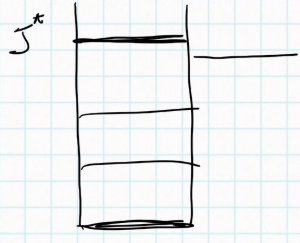
\includegraphics[scale=0.9]{Immagini/0325_lv.png}
    \caption{Livelli energetici del $\ce{^{20}Ne}$; la linea all'esterno rappresenta la reazione $p+\ce{^{19}F}$}
    \label{0325_lv}
\end{figure}
\noindent Come per l'elettrone, anche il nucleo presenta dei livelli energetici; se prendiamo per esempio la reazione $p+\ce{^{19}F}\to\ce{^{20}Ne}$, possiamo osservare dal disegno in Figura \ref{0325_lv} che la reazione è molto vicina al $\ce{^{20}Ne}^*$ per cui:
$$p+\ce{^{19}F}\to\ce{^{20}Ne}^*\to \ce{^{16}O} + \alpha$$
Si tratta quindi di una reazione $a+X$ che produce $Y+b$ passando per uno stadio intermedio $Z^*$ detto \textit{compound nucleus}\index{compound nucleus@\textit{compound nucleus}}; questo tipo di processo viene denominato \textbf{processo risonante}\index{processo risonante}\footnote{Si osservi che la $\sigma$ di tale processo è diversa sia da quella della reazione $a+X\to Y+b$ sia da $a+X\to Z$.}.

\subsubsection{Analisi Semi-classica}
Iniziamo studiando il processo con un approccio semi-classico. Se definiamo con $b$ il parametro di impatto per il proiettile $a$ sul bersaglio $X$, abbiamo per la sezione d'urto (classica) $\sigma = \pi b^2$; tale parametro in meccanica quantistica è legato alla quantità di moto da $b = \ell \: \hbar/p\equiv \ell\,\lambdabar_{DB}$\footnote{Abbiamo definito $\lambdabar_{DB}\equiv \lambda_{DB}/2\pi = \hbar/p$.}. Supponiamo di poter trascurare gli spin ($\ell$ si conserva) e dividere la zona di interazione in \vir{fette} al variare del valore di $\ell$: $0\leq \ell \leq 1$ allora $\sigma = \pi\lambdabar^2_{DB}$, $1\leq \ell \leq 2$ allora $\sigma = 3\pi\lambdabar^2_{DB}$ (area della corona); per un generico $\ell$
$$\sigma = \pi [(\ell+1)\lambdabar_{DB}]^2 - \pi[\ell\lambdabar_{DB}]^2 = (2\ell +1) \pi\lambdabar^2_{DB}$$
Dalla conservazione, $\ell$ è lo stesso per $Z^*$, quindi $\sigma(\ell)$ è la sezione d'urto d'eccitazione di $Z$.\\
Se a questo punto consideriamo anche gli spin ($J_a$, $J_X$,$\ell\to J$), sarà necessario eseguire una media per cui:
$$\sigma = \pi\lambdabar_{DB}\,\frac{2J+1}{(2J_a+1)(2J_X+1)}\equiv \pi\lambdabar_{DB}^2\,g$$
Inoltre ogni livello ha un certo allargamento di riga distribuito come una Lorentziana $f(E)$\footnote{$$f(E)=\frac{\Gamma^2}{(E-E_R)^2+(\Gamma/2)^2}$$} di cui tenere conto nell'espressione di $\sigma$.\\
Per quanto riguarda $Z^*$, abbiamo la possibilità sia che decada in $b+Y$ sia che faccia scattering elastico $a+X$, per cui ci sarà una certa probabilità di decadimento nell'$i$-esimo canale $P_i = \Gamma_i/\Gamma$, dove $\Gamma=\hbar/\tau$\footnote{$\tau$ tempo di decadimento.}; questa entra nella sezione d'urto per cui $\sigma\propto \Gamma_a\Gamma_b/\Gamma^2$. Si ottiene infine un'espressione per $\sigma$ detta \textbf{formula di \BW}\index{formula di \BW}\footnote{Abbiamo usato $p^2 = 2\mu E$.}:
$$\sigma = \pi\frac{\hbar^2}{2\mu E}g\Gamma_a\Gamma_b \frac{1}{(E-E_R)^2+(\Gamma/2)^2}$$

\subsubsection{Analisi Quantistica}
\begin{figure}[h]
    \centering
    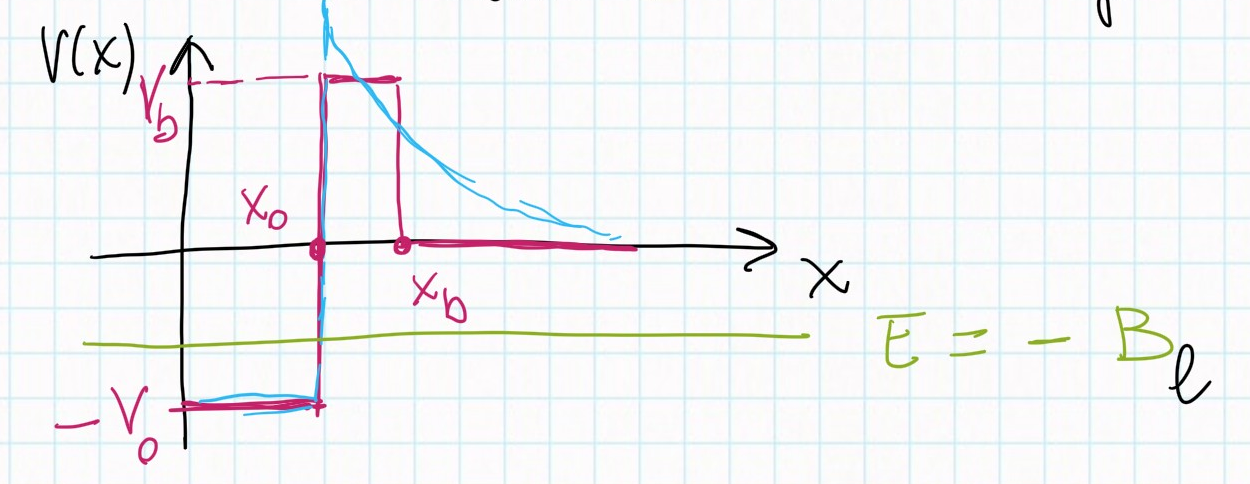
\includegraphics[scale=0.2]{Immagini/0325_pot.png}
    \caption{Schema della barriera di potenziale.}
    \label{0325_pot}
\end{figure}
\noindent Studiamo a questo punto il processo con l'approccio della meccanica quantistica\footnote{\label{0325_art}Si segue il calcolo riportato nell'articolo Charity, R.J., Eur. Phys. J. Plus, 2016, vol.131, art.63, \texttt{DOI:} \doi{10.1140/epjp/i2016-16063-1}.\articolo{Charity}}, servendoci però di un semplice \vir{modellino} unidimensionale a singola particella (come nel modello \textit{a shell}\index{modelli nucleari! a shell@\textit{a shell}} i nucleoni si muovono in un potenziale medio comune per tutti) dove non facciamo distinzione tra protoni e neutroni e rappresentiamo la barriera di potenziale come un \vir{muro} (Figura \ref{0325_pot}). Studiamo l'equazione di \Sch{} e le relative soluzioni per le varie zone ($x\lessgtr x_0,x_b$) per lo stato legato $E=-B_\ell$:
\begin{displaymath}
\begin{aligned}
\text{Equazioni}& & & \\
&1. & &-\frac{\hbar^2}{2m} \frac{d^2}{dx^2} \psi(x) = E\psi(x) & &x>x_b \\
&2. & &\ppc{-\frac{\hbar^2}{2m} \frac{d^2}{dx^2} + V_b} \psi(x) = E\psi(x) & &x_0<x<x_b \\
&3. & &\ppc{-\frac{\hbar^2}{2m} \frac{d^2}{dx^2}-V_0} \psi(x) = E\psi(x) & &x<x_0 \\
\text{Soluzioni}& & & \\
&1. & &\psi(x) = G\,e^{-k_\infty x} + \cancel{F\,e^{k_\infty x}} & &x>x_b \\
&2. & &\psi(x) = C\,e^{k_b x} + D\, e^{-k_b x} & &x_0<x<x_b \\
&3. & &\psi(x) = A\,\sin{(k_0x)} + \cancel{B\,\cos{(k_0x)}} & &x<x_0 
\end{aligned}
\end{displaymath}
$$k_0 \equiv \frac{\sqrt{2m(V_0-B_\ell)}}{\hbar}\qquad\quad k_b\equiv\frac{\sqrt{2m(V_b+B_\ell)}}{\hbar}\qquad\quad k_\infty\equiv\frac{\sqrt{2mB_\ell}}{\hbar}$$
Per trovare i vari coefficienti e $B_\ell$ si impone la continuità della funzione e della derivata prima e la normalizzazione. In Figura \ref{0325_ris} abbiamo riportato i risultati per $A=5$ nel fondamentale. 
\begin{figure}[!hb]
    \centering
    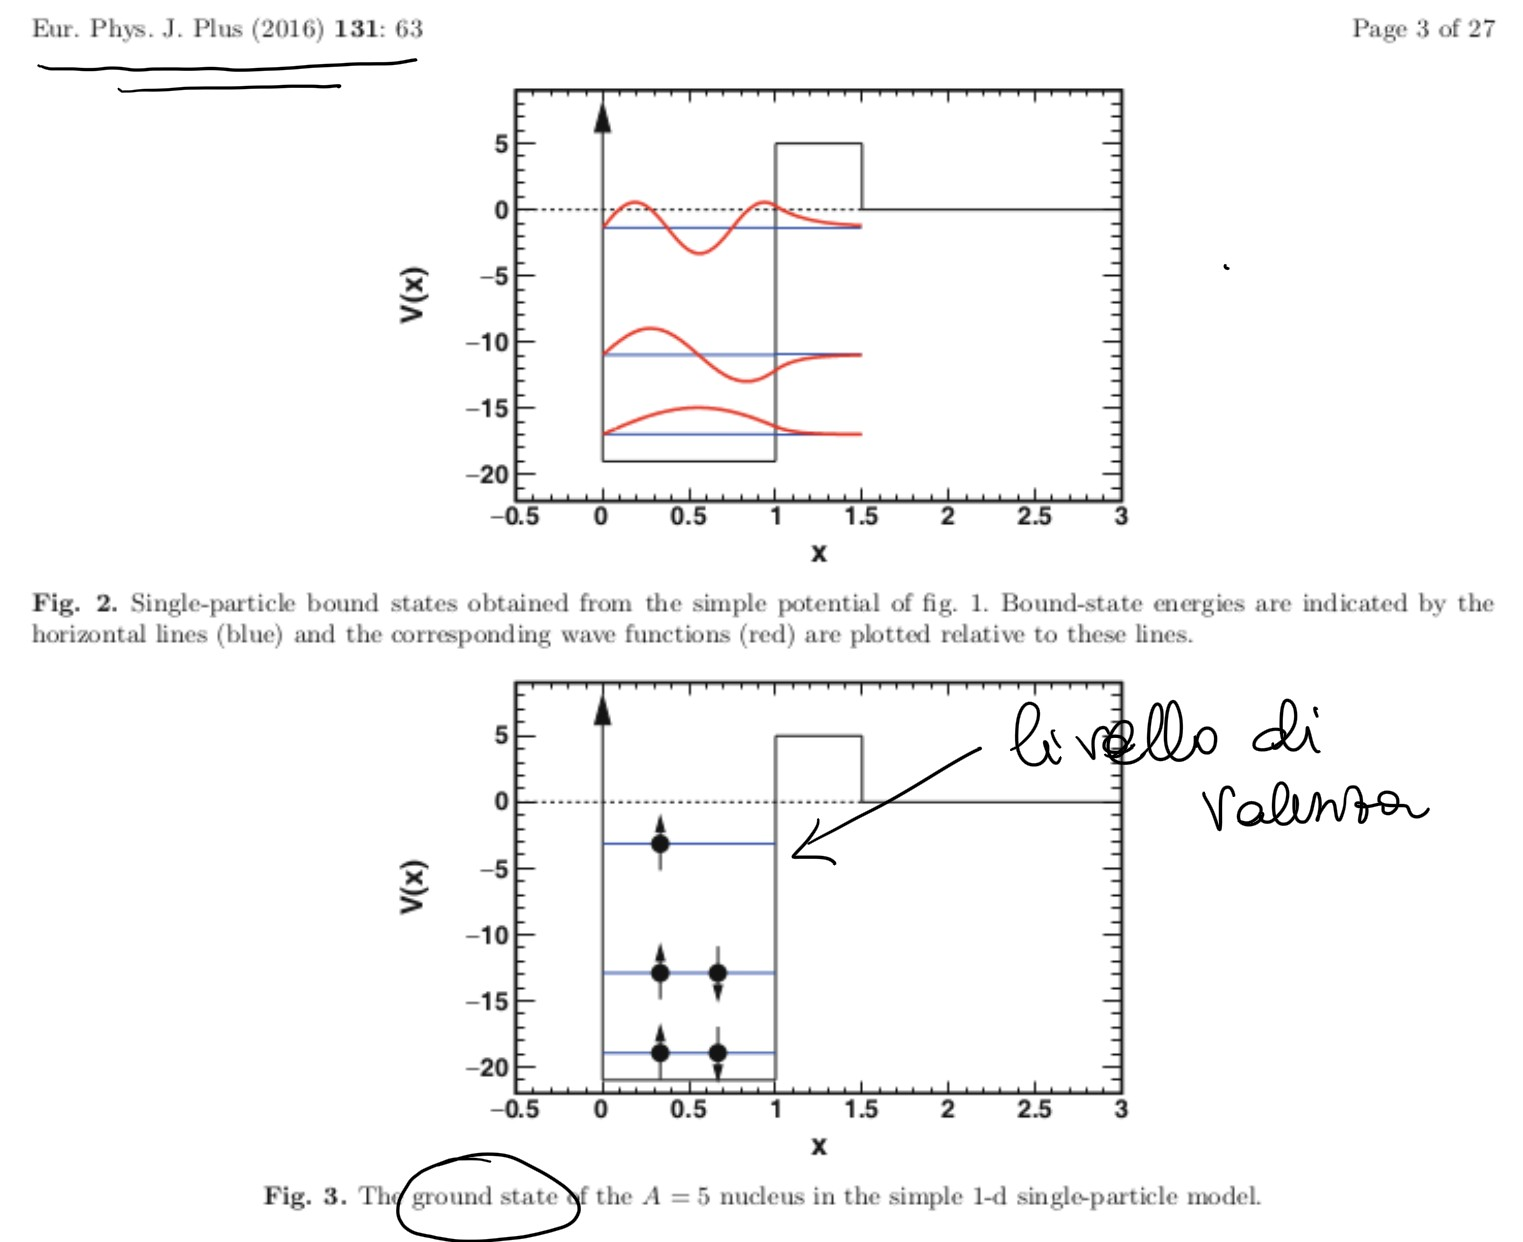
\includegraphics[scale=0.3]{Immagini/0325_risonanza.png}
    \caption{Grafici del potenziale e delle soluzioni del calcolo riportato nell'articolo.}
    \label{0325_ris}
\end{figure}
\noindent Come si ottiene lo stato eccitato? Si potrebbe promuovere un nucleone dal secondo livello a quello di valenza\index{livello di valenza}, ma questo non sarebbe lo stato risonante. Osserviamo però che modificando $V_0$ (cioè \vir{alzandolo}) si potrebbe fare in modo che l'energia del livello di valenza\index{livello di valenza} divenga positiva, ma rimanga inferiore a $V_b$ (Figura \ref{0325_potris}); esiterebbe allora una certa probabilità di \textit{tunneling}\footnote{$P_{tunnel} = 1 - P_{stay}$.} per quel nucleone:
$$\frac{dP_{stay}}{dt} = -\Gamma \, P_{stay} \quad \Rightarrow \quad P_{stay}\propto e^{-\Gamma t}$$
\begin{figure}[h]
    \centering
    \includegraphics{Immagini/0325_po_risonanza.png}
    \caption{Schema dello stato risonante.}
    \label{0325_potris}
\end{figure}
\noindent Dobbiamo allora considerare l'equazione di \Sch{} in funzione del tempo\footnote{$$i\hbar \frac{d\psi}{dt}(x,t) = \ppc{-\frac{\hbar^2}{2m}\frac{d^2}{dx}+V}\psi(x,t)$$} e cercare una soluzione del tipo $\psi(x,t) = \exp{(-i t \, E/\hbar)}\,\psi(x)$, dove $\psi(x)$ è soluzione dell'equazione di \Sch{} precedente. Ora l'andamento di $P_{stay}$ impone\footnote{$P_{stay}\propto |\psi(x,t)|^2 = |\exp{(-i t \, E/\hbar)}|^2\,|\psi(x)|^2$} che $E\in \C$, per cui scegliamo $E = E_R - i \Gamma/2 \:\Rightarrow\: |\psi(x,t)|^2 = \exp{(-t\Gamma/\hbar)}\,|\psi(x)|^2$. Osserviamo che il termine di dipendenza temporale si fa sentire solo per $x>x_b$ (Figura \ref{0325_ris2}), dunque:
$$x>x_b \qquad \psi(x,t) = H\,e^{i\,(-\frac{E}{\hbar}\,t + i\,k_\infty x)}$$
\begin{figure}[h]
    \centering
    \includegraphics[scale=0.4]{Immagini/0325_risonanza2.png}
    \caption{Grafici del potenziale e delle soluzioni del calcolo riportato nell'articolo.}
    \label{0325_ris2}
\end{figure}
\noindent Questo non è quindi uno stato eccitato, ma una \textbf{risonanza}\index{processo risonante}\index{risonanza}. Dal punto di vista dello scattering, siamo interessati al processo inverso, ovvero all'effetto \textit{tunnel}\index{effetto tunnel} per entrare; dall'equazione di \Sch{}:
\begin{displaymath}
\begin{aligned}
\psi(x)&= A\, \sin{(k_\infty x +\delta)} = & &x>x_b \\
&= \frac{A}{2i} \, e^{-i\delta}\ppc{e^{i\,(k_\infty x + 2\delta)} - e^{-i\,k_\infty x}} & \\
\psi(x)&= C\, e^{k_b x} + D\, e^{-k_b x} & &x_0<x<x_b \\
\psi(x)&= A'\, \sin{(k_0 x)} & &x<x_0 
\end{aligned}
\end{displaymath}
La probabilità di penetrazione sarà data da $P_{in}\propto \int_0^{x_0} |\psi(x)|^2 dx$ e ne osserviamo i risultati in Figura \ref{0325_ris3}.
\begin{figure}[h]
    \centering
    \includegraphics[scale=0.4]{Immagini/0325_risonanza3.png}
    \caption{Andamenti della probabilità di penetrazione e dello sfasamento in funzione dell'energia.}
    \label{0325_ris3}
\end{figure}
\noindent Si noti che l'andamento di $P_{in}\propto \Gamma^2/((E-E_r)^2+\Gamma^2/4)$ con $E_r$ energia del picco e $\Gamma = \,$FWHM e in particolar modo che per $E=E_r$ $\delta$ ha un salto di $\pi$ (questo è uno degli indicatori della presenza di una risonanza). Si ritrova allora la \BW\index{formula di \BW}.

\newpage

\subsubsection{Reaction-rate e fattore astrofisico}
Sostituiamo allora in $\mean{\sigma v}$ l'espressione di \BW{} per $\sigma$\footnote{Attenzione nelle note del corso vi è un errore: è riportato un $-$ al denominatore, invece di un $+$.}:
\begin{displaymath}
\begin{aligned}
\mean{\sigma v} &= \sqrt{\frac{8}{\pi\mu}} \ppc{\frac{1}{kT}}^{3/2} \frac{\pi\hbar^2}{2\mu} g \Gamma_a\Gamma_b \int_0^\infty \frac{1}{(E-E_R)^2 + (\Gamma/2)^2} \, e^{-E/kT} dE \simeq \\
&\simeq \sqrt{2\pi}\ppc{\frac{1}{\mu kT}}^{3/2} g\hbar^2 \Gamma_a\Gamma_b\, e^{-E_R/kT} \int_0^\infty \frac{dE}{(E-E_R)^2 + (\Gamma/2)^2} =\\
&= \sqrt{2\pi}\ppc{\frac{1}{\mu kT}}^{3/2} g\hbar^2 \Gamma_a\Gamma_b\, e^{-E_R/kT} \,\frac{2}{\Gamma} \arctan{(\frac{2}{\Gamma}(E-E_R))}\Bigr |_{0}^\infty \simeq \qquad \frac{E_R}{\Gamma}\to \infty \\
&\simeq \sqrt{2\pi}\ppc{\frac{1}{\mu kT}}^{3/2} g\hbar^2 \Gamma_a\Gamma_b\, e^{-E_R/kT} \, \frac{2\pi}{\Gamma} = \\
&= \ppc{\frac{2\pi}{\mu kT}}^{3/2} \hbar^2 \ppc{g\frac{\Gamma_a\Gamma_b}{\Gamma}}e^{-E_R/kT}
\end{aligned}
\end{displaymath}
dove abbiamo approssimato $\exp{(-E/kT)}\sim \exp{(-E_R/kT)}$, perché $E_R\gg \Gamma \sim 1$ eV e la distribuzione è molto piccata intorno $E_R$. Studiamo anche il fattore astrofisico\index{fattore astrofisico@fattore astrofisico $S(E)$}:
$$S(E)=E\, \sigma(E) \, e^{2\pi\frac{Z_1Z_2e^2}{\hbar v}}= \frac{\pi}{2\mu} \hbar^2 g \frac{\Gamma_a\Gamma_b}{(E-E_R)^2+(\Gamma/2)^2}e^{b/\sqrt{E}}$$
Prendiamo a titolo di esempio la reazione $p+\ce{^7Be}\to \ce{^8B} +\gamma$: $E_R=700$ keV, $\Gamma_p \simeq 35$ keV, $\Gamma_\gamma \simeq 25$ meV (trascurabile, $\Gamma \sim \Gamma_p$) e $b=0.99\cdot 3\,\sqrt{7/8}\unit{MeV}^{1/2}$. 

\paragraph{Tipologie di risonanze} Le risonanze si dividono principalmente in due tipologie in base al rapporto $\Gamma/E_R$:
\begin{itemize}
    \item \textbf{strette}\index{risonanza!stretta} $\Gamma/E_R<10\%$.
    \item \textbf{larghe}\index{risonanza!larga} $\Gamma/E_R>10\%$.
\end{itemize}
Il tipo di risonanza può essere significativo nello studio del fattore astrofisico\index{fattore astrofisico@fattore astrofisico $S(E)$}: se infatti la risonanza è stretta, nel caso in cui il \textit{range} di interesse sia lontano dal valore di risonanza le misure non risentono di alcun effetto del picco; al contrario con una risonanza larga, si possono avere effetti dovuti alle code della risonanza che alterano le acquisizioni (per esempio si registrano valori maggiori di quelli attesi senza la risonanza).

\subsubsection{Risonanze sotto soglia}
\begin{figure}[h]
    \centering
    \includegraphics[scale=0.8]{Immagini/0325_risonanza4.1.png}
    \caption{Schema risonanza sotto soglia}
    \label{0325_ris41}
\end{figure}
\noindent Esiste anche un particolare tipo di risonanza detta \textbf{risonanza sotto soglia}\index{risonanza!sotto soglia}, per cui tra i livelli del \textit{compound nucleus}\index{compound nucleus@\textit{compound nucleus}} compare uno stato risonante sotto alla soglia della reazione (Figura \ref{0325_ris41}); se la risonananza è sufficientemente larga può influenzare le misure portando per esempio a un piccolo andamento crescente (\vir{una risalita}) del fattore astrofisico\index{fattore astrofisico@fattore astrofisico $S(E)$} per energie prossime a $E=0$ (Figura \ref{0325_ris4}). Questo dimostra l'importanza di una buona guida teorica nella zona di estrapolazione.

\begin{figure}[h]
    \centering
    \includegraphics[scale=0.3]{Immagini/0325_risonanza4.png}
    \caption{Simulazione di una situazione sperimentale con risonanza sotto soglia. $E_{Th}$ è la minima energia raggiunta dagli esperimenti diretti.}
    \label{0325_ris4}
\end{figure}
\newpage
\subsubsection{Risonanza e neutrini solari}\label{0325-sec-risnu}
Abbiamo già studiato nella sezione \secrif{0322-sec-nu} come la questione dei neutrini solari, prima degli esperimenti di rivelazione delle oscillazioni di sapore, fosse un problema alquanto discusso\complementi{l'ipotesi di Fowler}. Tra le varie teorie avanzate ve ne fu una anche da parte di Fowler che prevedeva appunto la possibilità di una risonanza non studiata: egli supponeva che il calcolo del fattore astrofisico fosse sbagliato a causa di una risonanza o sotto soglia\index{risonanza!sotto soglia} o molto stretta\index{risonanza!stretta} nella reazione $\ce{^3He}+\ce{^3He}$ ($ppI$) nel \textit{range} di energie di interesse astrofisico (che nel 1980 non era ancora stato esplorato); dunque il valore di $S(E)$ sarebbe stato sottostimato. Tale soluzione, però, fu confutata dalle misure di LUNA\esperimento{LUNA}\footnote{Guarda \secrif{sec-LUNA-I}.} che dimostrarono l'assenza di qualsiasi tipo di risonanza.    %   25/03
%%  Elettroscreening
%\part*{Lezione 29/03/2021}
\subsection{Elettroscreening}\label{0329-sec-screening}
Passiamo alla trattazione\footnote{Calcolo ripreso dall'articolo Salpeter, E.E., Australian Journal of Physics, 1954, vol.7, p.373, \texttt{DOI:} \doi{10.1071/PH540373}.\articolo{Salpeter}} del fenomeno dell'elettroscreening\index{elettroscreening}: immaginiamo l'atomo come un gas con una alta densità nel centro, dove si concentrano tutte le cariche positive; questo comporta una nuvola polarizzata che scherma il potenziale coulombiano (screening potenziale). Si ha allora una modifica nel termine di Gamow\index{picco di Gamow} $P(E)$ in $\mean{\sigma v}$:
$$U_{tot} (r) = \underbrace{\frac{Z_1Z_2e^2}{r}}_{U_{coul}} + U(r)$$
Definiamo allora alcune quantità che ci serviranno nel calcolo del contributo del termine $U(r)$:
\begin{itemize}
    \item $E_{\max{}}\gg kT$ è l'energia del picco di Gamow.
    \item $r_C$ è il \textit{classical turning point}\index{classical turning point@\textit{classical turning point}}, ovvero il raggio per cui $E_{\max{}} = Z_1Z_2e^2/r_C$.
    \item $r_n\ll r_C$ è il raggio nucleare, distanza dalla quale il potenziale attrattivo nucleare diviene maggiore della repulsione coulombiana.
    \item $a$ è la grandezza scala della distanza tra le particelle. Data $\rho$ la densità del gas e $N_0$ il numero di Avogadro\index{numero di Avogadro}, definiamo $a$ come quel valore per cui:
    $$4\pi a^3\,\rho N_0 =1 \;\Rightarrow\; 4\pi a^3 \tilde{\rho} = 1$$
    Dal momento che\footnote{Se $M$ è misurata in a.m.u..} $\tilde{\rho} = 3M/4\pi a^3$, si ha $M= 1/3$ a.m.u., ovvero $a$ può essere visto come il raggio di una sfera di massa media pari a un terzo di unità di massa atomica.
    \item $R$ è il raggio della nuvola elettronica (vedremo che $R>a$ e $R\gg r_C$, altrimenti non si avrebbe lo screening).
\end{itemize}
Per capire come si modifica $P(E)$ dobbiamo studiare $E-U(r)-Z_1Z_2e^2/r$. Per $r\gg R$ ovviamente $U(r)\ll 1$ possiamo quindi approssimarlo come costante $U_0 \simeq Z_1Z_2e^2/R = E_{\max{}}\, r_C/R\ll1$.
\begin{figure}[!h]
    \centering
    \includegraphics[scale=0.3]{Immagini/0329_pot_ES.png}
    \caption{Schema della barriera di potenziale con (linea nera) e senza (linea rosa) elettroscreening\index{elettroscreening}.}
    \label{0329_schema}
\end{figure}
\noindent Come mostrato in Figura \ref{0329_schema} l'effetto dell'elettroscreening\index{elettroscreening} è quello di abbassare la barriera di potenziale ed è possibile descrivere il problema nel caso di assenza di elettroscreening\index{elettroscreening} \textit{shiftando} l'energia $E\to E+U_0$; l'integrale allora diviene\footnote{Abbiamo approssimato l'estremo inferiore dell'integrale $U_0$ a 0, poiché $U_0/E_{\min{}}\ll1$.}:
$$\int_0^\infty dE\, S(E+U_0) P(E+U_0) e^{-(E+U_0)/kT}\: \stackrel{U_0\ll E_{\max{}}}{\simeq} e^{-U_0/kT}\PPq{\int_0^\infty dE\, S(E) P(E) e^{-E/kT}}$$
Alcuni valori tipici:
\begin{displaymath}
\begin{aligned}
r_n &\simeq 2\unit{fm} = 2\cdot\ord{-13}\unit{cm} & a   &\simeq \ord{-9}\unit{cm}\\
r_C &\simeq 2\cdot\ord{-11}\unit{cm} & R   &\simeq 3\cdot\ord{-9}\unit{cm}
\end{aligned}
\end{displaymath}
Per semplicità supponiamo che $Z_1>Z_2$ e $z\equiv Z_2$ sia la carica dei costituenti principali del gas stellare.\\ Abbiamo allora due possibili effetti:
\begin{enumerate}
    \item \textbf{screening forte}\index{elettroscreening!forte} $E_{coul} > kT$ che riguarda principalmente gli esperimenti di fusione con plasma e che anche se trattati nell'articolo di Salpeter non discuteremo.
    \item \textbf{screening debole}\index{elettroscreening!debole} $E_{coul}\ll kT$ che interessa principalmente le stelle.
\end{enumerate}

\subsubsection{Calcolo screening debole}
Ancora una volta definiamo alcune quantità utili:
\begin{itemize}
    \item[-] Il numero medio di elettroni per a.m.u. nel gas stellare: 
    $$\xi \equiv \sum_i \frac{X_iZ_i}{A_i}$$
    dove con $X_i$ si intende l'abbondanza frazionale in massa\index{abbondanza frazionale in massa}\index{fractional abundance} del nucleo $i$ con carica $Z_i$ e numero di massa $A_i$.
    \item[-] L'energia di Fermi del gas di elettroni nel caso non relativistico:
    $$E_F \equiv \frac{h^2}{8\pi^2 m}(3\pi^2N_0\rho\, \xi)^{2/3} = \ppc{\frac{3\pi\xi}{4}}^{2/3} \ppc{\frac{h}{a}}^2 \frac{1}{8\pi^2m}$$
    \item[-] Infine definiamo il rapporto:
    $$D\equiv \frac{E_F}{kT} \simeq 0.30 \frac{(\xi\rho)^{2/3}}{T_6}$$
\end{itemize}
Nel caso di screening debole\index{elettroscreening!debole} supponiamo che il gas di elettroni sia non degenere e che i costituenti principali del gas stellare abbiano $z$ e $A$; allora si ha:
$$U_{tot}(r) = Z_1 z e^2 \psi_{tot}(r)$$
$$\psi_{tot}(r) \equiv \frac{1}{r} + \psi(r)$$
Mettiamoci con $Z_1$ nel centro e con $V(r)$ potenziale elettrostatico e $\bar{\rho}(r)$ densità di carica elettronica mediati su tutte le particelle eccetto 1. Per una carica di prova $\delta Z\,e$ si ha dall'equazione di Poisson\footnote{$\nabla^2 V(r) = -4\pi{\rho}(r)$.}:
\begin{equation}\label{0329_poisson}
    \nabla^2 Z_1 e\,\psi_{tot}(r) = -4\pi\bar{\rho} -4\pi \,Z_1 e\delta^{3}(r)
\end{equation}
Per risolvere il sistema abbiamo però bisogno di un'altra equazione, che ci viene data dalla meccanica statistica:
consideriamo una regione in cui ogni particella ha energia potenziale $U_e(r)$, allora la densità di carica media sarà data da:
\begin{equation*}
    \bar{\rho} (r) = \underbrace{\ppc{\frac{\rho N_0ze}{A}}}_\text{densità di carica}\:\PPq{\underbrace{\exp{\ppc{-\frac{Z_1ze^2}{kT}\psi_{tot}(r)}}}_\text{parte nucleare} - \underbrace{\exp{\ppc{\frac{Z_1e^2}{kT}\psi_{tot}(r)}}}_\text{parte elettronica}}
\end{equation*}
Nel caso di screening debole possiamo sviluppare gli esponenziali al prim'ordine per cui l'espressione diviene:
\begin{equation}\label{0329_rho}
    \bar{\rho} (r) \simeq - \ppc{\frac{\rho N_0ze}{A}}\: \psi_{tot}(r) \frac{Z_1e^2}{kT} (1+z)
\end{equation}
Allora sostituendo questa in \eqref{0329_poisson} abbiamo:
$$\nabla^2 \ppc{\cancel{\frac{1}{r}} + \psi(r)} = 4\pi \rho N_0 \frac{e^2(z+z^2)}{A\, kT}  \ppc{\frac{1}{r} +\psi(r)} \cancel{-4\pi \delta^3(r)}$$
\begin{equation}\label{0329_eq}
    \nabla^2 \psi(r) = 4\pi \rho N_0 \frac{e^2(z+z^2)}{A\, kT}  \ppc{\frac{1}{r} +\psi(r)}
\end{equation}
Le condizioni al contorno per questa equazione differenziale sono imposte dalla necessità di avere il potenziale $\propto 1/r$ per grandi distanze e finito per $r=0$:
\begin{displaymath}
\begin{aligned}
&r\to +\infty & &\psi(r) \to -\frac{1}{r}\\
&r\to 0 & &\psi(r) \to \psi(0)<\infty
\end{aligned}
\end{displaymath}
Per semplicità definiamo $R_{DH}$\footnote{Dall'analisi dimensionale $[R_{DH}] = [L]$. Le lettere a pedice indicano le iniziali di Debye e \Huckel{}, questa scelta fu fatta da Salpeter poiché le soluzioni di questo problema erano le stesse di quelle della teoria delle soluzioni diluite elettrolitiche, costruita dai due scienziati\complementi{la teoria di Debye-\Huckel}.} in modo da raccogliere tutti i termini costanti in \eqref{0329_eq}:
$$R_{DH}^2 \equiv \frac{kT}{4\pi \rho N_0e^2} \frac{A}{z+z^2} = \frac{kT}{e^2} a^3 \frac{A}{z+z^2}$$
La soluzione è data da\footnote{$$\nabla^2 \psi(r) = \ppc{\frac{d^2}{dr^2} + \frac{2}{r}\frac{d}{dr}}\psi(r)\: \Rightarrow\: \frac{d^2\Psi}{dr^2} - \frac{1}{R_{DH}^2}\Psi = \frac{1}{R_{DH}^2} $$%
con $\Psi (r) \equiv r\,\psi(r)$ per cui $\Psi \to -1$ per $r\to+\infty$ e $\Psi \to 0$ per $r\to 0$.}:
$$\psi(r) = \frac{1}{r}\ppc{e^{-r/R_{DH}}-1}$$
Notiamo che $\psi(0)\simeq (1-r/R_{DH}-1)/r=-1/R_{DH}$ e $\psi(r\to\infty)=-1/r$. Avremo allora per l'energia potenziale $U(r) = Z_1Z_2 e^2 \psi(r)$:
$$U(r) = Z_1Z_2 e^2 \frac{1}{r} \ppc{e^{-r/R_{DH}}-1} \qquad U(0)=U_0 = -\frac{Z_1Z_2 e^2}{R_{DH}}$$
\begin{equation}\label{0329_U0}
-\frac{U_0}{kT}\simeq 0.188 Z_1Z_2 \sqrt{\frac{\rho}{T_6^3}}\,\xi
\end{equation}
dove abbiamo definito $\xi\equiv \sqrt{(z+z^2)/A}$.

\paragraph{Un calcolo più preciso.}Rilassiamo a questo punto alcune delle ipotesi fatte in precedenza. Consideriamo un gas a più specie nucleari $z_i, A_i, X_i$, per cui\footnote{\acc{E} sufficiente mandare $z^2/A$ in $\sum_i X_iz^2_i/A_i$.}:
$$\bar{\rho}(r)\propto \sum_i \exp{\ppc{-Z_1 \frac{z_iX_i e^2}{kT}\psi_{tot}(r)}}$$
Inoltre dal momento che sono fermioni consideriamo gli elettroni distribuiti come una Fermi-Dirac\index{distribuzione di Fermi-Dirac}:
$$f(\eta) = \int_0^\infty dx \frac{\sqrt{x}}{e^{x-\eta}+1}$$
con $\eta \equiv \mu/kT$; per elettroni non interagenti $f(\eta) = 2D^{2/3}/3$. Poiché la densità degli elettroni si aggiusta in modo tale da uniformare il potenziale termodinamico, per elettroni interagenti avremo:
\begin{displaymath}
\begin{aligned}
f\ppc{\eta - \frac{U_e(r)}{kT}} &= \int_0^\infty dx \frac{\sqrt{x}}{e^{x-\eta}e^{U_e/kT}+1} \simeq \\
&\simeq \int_0^\infty dx \frac{\sqrt{x}}{e^{x-\eta}\ppc{1+U_e/kT}+1} =\\
&= \int_0^\infty dx \frac{\sqrt{x}}{\ppc{e^{x-\eta}+1}\ppc{1+\frac{U_e}{kT}\frac{e^{x-\eta}}{e^{x-\eta}+1}}}\simeq \\
&\simeq \int_0^\infty dx \frac{\sqrt{x}}{e^{x-\eta}+1}\ppc{1-\frac{U_e}{kT}\frac{e^{x-\eta}}{e^{x-\eta}+1}} =\\
&= f(\eta) - \frac{U_e}{kT}\frac{df}{d\eta}\:\footnotemark
\end{aligned}
\end{displaymath}
\footnotetext{$$\frac{df}{d\eta} = -\int_0^\infty dx \frac{\sqrt{x}}{(e^{x-\eta}+1)^2} (-e^{x-\eta})$$}
\noindent Il rapporto tra gli elettroni interagenti e quelli non interagenti sarà dato da:
$$\frac{f(\eta-U_e/kT)}{f(\eta)} \simeq 1- \frac{U_e}{kT}\frac{f'(\eta)}{f(\eta)}$$
Questo termine entra nell'espressione di $\bar{\rho}$ influendo sul rapporto $z/A$, per cui adesso avremo la stessa espressione \eqref{0329_U0}, ma $\xi$ sarà definito come\footnote{Ovviamente è necessario conoscere $X_i$; fino a qualche anno fa non c'erano problemi, ma negli ultimi tempi nuove misure per il Sole hanno sollevato tensioni sui valori.}:
$$\xi^2 \equiv \sum_i\frac{X_iz_i^2}{A_i} + \frac{f'(\eta)}{f(\eta)}\sum_i\frac{X_iz_i}{A_i}$$

\subsubsection{In laboratorio}
Studiamo allora gli effetti dell'elettroscreening\index{elettroscreening}.\\
Prendiamo un nucleo proiettile $A_1$ (per es. ioni di un nucleo) e un nucleo bersaglio $A_2$ (per es. una targhetta o un gas) per cui si ha:
$$A_1+A_2 \to A_3 + \gamma$$
Per esempio $p+\ce{^7Be}$. Dato che il nucleo è circondato dalla nuvola elettronica avremo un certo effetto di screening, tuttavia non si tratta dell'effetto di interesse astrofisico, poiché le densità stellari sono differenti da quelle ottenibili in laboratorio; non siamo quindi interessati alla sezione d'urto con lo screening ($\sigma_{lab}$), ma a quella priva di esso ($\sigma_{bare}$). Definito $\eta(E)\equiv Z_1Z_2e^2/\hbar v$, abbiamo dalla teoria:
$$\sigma_{lab}(E) = \frac{S(E)}{E}e^{-2\pi \eta(E)}$$
Poiché\footnote{Si tenga a mente che $U_0^{lab}\not= U_{0}^{star}$.} $U_0\ll E_{\max{}}$, detta $E_{eff}\equiv E+U_0$ si ha che $S(E)/E\approx S(E_{eff})/E_{eff}$, per cui:
$$\frac{\sigma_{lab}(E)}{\sigma_{bare}(E)} \simeq \frac{e^{-2\pi\eta(E_{eff})}}{e^{-2\pi\eta(E)}}$$
Facendo uno sviluppo per $\eta(E_{eff})$ in un intorno di $E$ e notando che $d\eta/dE = -\eta(E)/2E$ otteniamo:
$$\frac{\sigma_{lab}(E)}{\sigma_{bare}(E)} \simeq \exp{\ppc{\pi Z_1Z_2e^2 \sqrt{\frac{2\mu}{E}}\frac{U_0}{E}}}\equiv e^{g(E)}$$
Dunque per basse energie è necessario \vir{pulire} la $\sigma$ misurata secondo quell'esponenziale e poi da questa calcolarsi la $\sigma$ per i modelli stellari.\\
Solitamente $U_0\approx Z_1Z_2 e^2/R_a$ con $R_a$ raggio atomico, per cui quello che viene fatto è \textit{fittare} i dati con $U_0$ come parametro; se osserviamo per $E\to0$ un andamento crescente di tipo lorentziano abbiamo una risonanza (o stretta o sotto soglia), se invece tale andamento è $\sim \exp{(g(E))}$ allora siamo in presenza di elettroscreening\index{elettroscreening}. In ultima battuta osserviamo che minore è l'energia alla quale osserviamo e maggiore sarà la sensibilità dell'andamento a possibili effetti di screening.
    %   29/03
%%  Studio pp con Ab Initio
%   Articolo di Bethe
%\part*{Lezione 31/03/2021}
\section{Studio \textit{ab-initio}}\label{0331-sec-studioab}\index{Metodo ab-initio@Metodo \textit{ab-initio}}
La $pp$ non si riesce a misurare, tuttavia è possibile studiarla\footnote{Avvertiamo il lettore che ci saranno differenze di notazione rispetto a quando abbiamo mostrato il calcolo la prima volta.} col metodo che abbiamo discusso nella sezione \secrif{0318-sec-abinitio}; fu Bethe il primo a lavorarci, dando inizio al modello solare.\\
Prima di \vir{addentrarci} nel calcolo, osserviamo che la funzione d'onda finale sarà la stessa di quella per lo studio della reazione in sezione \secrif{0317-sec-abinitio}, poiché il prodotto di entrambe è un deutone, tuttavia si avranno differenze per le funzioni d'onda dei reagenti e per il fatto che la $pp$ non è mediata dall'interazione elettromagnetica.
$$p+p \to d+e^++\nu_e$$
Dunque studieremo la cinematica della reazione per avere la dipendenza dall'elemento di matrice ridotta e poi passeremo al calcolo di questo. 

\paragraph{Calcolo della cinematica.}Detto $w$ il \textit{rate} di decadimento, dalla teoria di Fermi\index{regola d'oro di Fermi}:
$$w = \frac{2\pi}{\hbar}|V_{fi}|^2\rho(E_f)$$
dove $V_{fi} = G_F M$ con $G_F$ costante di Fermi\index{costante di Fermi@costante di Fermi $G_F$}\index{costante di accoppiamento debole@costante di accoppiamento debole $g$} e $M$ elemento di matrice del decadimento $\beta^+$. Trascuriamo la massa del neutrino per cui $E_i-E_f\equiv E_0 = E_e + E_\nu = E + cq$ e nel centro di massa $\vec{p}_d = -\vec{p}-\vec{q}$ (non indipendente da $p$ e $q$, ma determinato da essi); possiamo allora riscrivere la densità di stati finali nello spazio delle fasi:
\begin{displaymath}
\begin{aligned}
dn &= \frac{d^3 p}{(2\pi\hbar)^3}\frac{d^3 q}{(2\pi\hbar)^3} =\\
&= \frac{p^2 q^2}{4\pi^4 \hbar^6} dpdq\: \footnotemark \\
\rho(E_f)\equiv \frac{dn}{dE_\nu} = \frac{dn}{cdq} &= \frac{p^2 (E_0-E)^2}{4\pi^4 c \hbar^6\,c^2} dp
\end{aligned}
\end{displaymath}
\footnotetext{Abbiamo integrato su $d\hat{q}d\hat{p}$.}
dove ci siamo limitati solo agli stati di interesse $dn/dE_\nu$ (come avevamo fatto nel decadimento $\beta$ fissando l'energia dell'elettrone e differenziando in $q$). Avremo quindi per il \textit{rate}:
$$dw = \frac{2\pi}{\hbar}|V_{fi}|^2\,\frac{p^2 (E_0-E)^2}{4\pi^4 c \hbar^6\,c^2} dp \stackrel{p\to E}{=} \frac{|V_{fi}|^2}{2\pi^3 \hbar^7 c^6} (E_0-E)^2 \sqrt{E^2 - m^2c^4} E dE $$
Ricordando che $d\sigma = dw/j_{inc} = dw/v$, integrando in $dE$ si ha\footnote{$c=\hbar=1$.}:
$$\sigma = \frac{1}{2\pi^3 v} G_F^2 |M|^2 \underbrace{\int_m^{E_0} (E_0-E)^2 \sqrt{E^2-m^2}E dE}_{\text{int. di Fermi } f(E_0)} $$\index{integrale di Fermi@integrale di Fermi $f(E_0)$}
$$|M|^2 \to \frac{1}{(2S_p +1)^2} \sum_{spin} |M|^2 = \frac{1}{4} \sum_{spin} |\int d^3x\: \psi^*_d (\vec{x})\,\psi_{pp}(\vec{x})|^2$$
dove abbiamo mediato sugli \textit{spin}\footnote{La parte di \textit{isospin} $\eta_d(\tau=0)(np)\sum_i\tau^-_i (pp)$ valutata sulle funzioni d'onda è 1.}. Da questo punto in poi adesso si procede numericamente, tuttavia a scopo illustrativo illustriamo il calcolo analitico che eseguì anche Bethe\footnote{L'articolo al quale ci riferiamo è Bethe, H. A. \& Critchfield, C. L., Phys. Rev., 1938, vol.54, p.248, \texttt{url:} \url{https://journals.aps.org/pr/abstract/10.1103/PhysRev.54.248}.\articolo{Bethe}}.

\paragraph{Risoluzione analitica.} Anche se il calcolo è analitico il risultato è piuttosto valido.\\
Per studiare $\psi_d$ prendiamo:
\begin{itemize}
    \item l'onda $S$ $\psi_d\to{^3S_1}$, per cui $\psi_d = u(r)/r$.
    \item buca di potenziale $V = -V_0$ per $r<r_0$.
    $$%
    \psi_d = \Bigl \{
    \begin{array}{llr}
        \frac{C}{r}\, e^{-\alpha r } & r>r_0 & \alpha\equiv \sqrt{mB}/\hbar \\
        \frac{C'}{r}\, \sin{(k_0 r)} & r<r_0 & k_0 \equiv \sqrt{m(V_0-B)}/\hbar
    \end{array}%
    $$
    Abbiamo allora $b\equiv 1/\alpha \simeq 4.4$ fm e definendo $x\equiv r/b$, $x_0\equiv r_0/b$ e $\mu \equiv \sqrt{(V_0-B)/B}=k_0/\alpha$ si ottiene:
    $$%
    \psi_d = \Bigl \{
    \begin{array}{ll}
        \frac{A}{r}\; e^{-(x-x_0)}\equiv \psi_> & r>r_0 \\
        \frac{A}{r}\; \sin{(\mu x)}/\sin{(\mu x_0)}\equiv \psi_< & r<r_0
    \end{array}%
    $$
    Osserviamo che questa espressione soddisfa automaticamente la continuità sia della funzione che della sua derivata in $r=r_0$, per cui dalla condizione di normalizzazione\footnote{$1=\int |\psi_d|^2=\int_0^{r_0}|\psi_<|^2+\int_{r_0}^\infty|\psi_>|^2$.} si ottiene\footnote{Successivamente per non confonderci con la costante che compare in $\psi_{pp}$ chiameremo questa $A\to A_d$.}:
    $$A = \frac{1}{\sqrt{2\pi b}}\, \frac{1}{\sqrt{1+x_0}}\,\frac{1}{\sqrt{1+\mu^{-2}}}$$
\end{itemize}
Studiamo a questo punto $\psi_{pp}$:
\begin{itemize}
    \item consideriamo sempre un'onda $S$ ($\ell=0$), perché le energie sono comunque basse\footnote{Si ricordi l'ordine di grandezza per le energie del picco di Gamow.}.
    \item prendiamo la stessa buca di potenziale, ma per $r>r_0$ consideriamo un potenziale coulombiano $V_{coul}$. Dovremo risolvere allora l'equazione di \Sch{} con $\psi_{pp} (r) = u(r)/r$:
    $$u'' - \frac{m}{\hbar^2} (V(r) - E)u =0$$
    Definita la massa ridotta $\mu\equiv m/2$ e $\rho\equiv kr$ con $k=\mu v /\hbar$ si ha\footnote{$E=\mu v^2/2 = \hbar^2 k^2/m$.} allora per $r<r_0$:
    $$\ppc{\frac{d^2}{d\rho^2} + 1 + \frac{2V_0}{\mu v^2}}u=0$$
    $$\psi_< (r) \: r = u(r) = A \, \sin{\ppc{\frac{\sqrt{mD}}{\hbar} r}} $$
    $$ D \equiv \underbrace{V_0}_{\sim\unit{MeV}} + \underbrace{\frac{\hbar^2k^2}{m}}_{\simeq 6\unit{keV}} \simeq V_0 $$
    Per quanto riguarda invece $r>r_0$ prendiamo le funzioni di Coulomb\footnote{Nel nostro caso $L=0$.}\index{funzioni di Coulomb} regolare $F_L(kr)$\index{funzioni di Coulomb!regolare} e irregolare $G_L(kr)$\index{funzioni di Coulomb!irregolare}:
    $$\psi_>(r) = \PPq{F_0 (kr) + \tan{(\delta_0)}\:G_0(kr)}\frac{e^{i\delta_0}\cos{(\delta_0)}}{kr}$$
    dove $\delta_0$ è lo sfasamento. Per trovare $A$ e $\delta_0$ imponiamo:
    \begin{itemize}
        \item continuità delle derivate logaritmiche:
        $$\frac{\psi_>'}{\psi_>}\Bigr |_{r=r_0} = \frac{\psi_<'}{\psi_<}\Bigr |_{r=r_0}$$
        $$\tan{\delta_0} = \frac{F_0(kr_0) - F_0(kr_0)\,\frac{d}{dr}\ln{w}(r_0)}{G_0(kr_0)\,\frac{d}{dr}\ln{w}(r_0) - G_0'(kr_0)}$$
        dove abbiamo definito $w(r) = A \sin{(\sqrt{mD}r/\hbar)}$.
        \item continuità delle funzioni in $r=r_0$:
        $$A \simeq \frac{F_0(kr_0)+\tan{\delta_0} G_0(kr_0)}{k\sin{(\sqrt{mD}r_0/\hbar)}}$$
        dove abbiamo approssimato $\cos{\delta_0}\sim e^{i\delta_0}\sim 1$ dal momento che $\delta_0\sim 0.002$.
    \end{itemize}
    Al tempo di Bethe $F_0$ e $G_0$ erano tabulate (non esistevano i calcolatori), per cui si aveva:
    $$F_0(kr)\simeq \underbrace{\sqrt{\frac{2\pi\gamma}{e^{2\pi\gamma}-1}}}_\text{Cost. Coulomb}kr\,\Phi(kr)\equiv C_0\, kr \, \Phi(kr) $$
    $$G_0(kr)=C_0^{-1} \, \Theta(kr)$$
    dove $\gamma \equiv Z_1Z_2e^2/\hbar v$ e $\Phi$ e $\Theta$ sono due polinomi tabulati\footnote{Non siamo interessati all'espressione di questi polinomi, ma la riportiamo solo per completezza:
    $$\Phi(kr)\simeq 1+\gamma\, kr - (2\gamma^2-1)\frac{(kr)^2}{6} + O((kr)^3) = \sum_{i=0}^\infty \varphi_i (kr)^i$$
    $$\Theta(kr) = \sum_{j=0}^\infty \theta_j (kr)^j + (2kr\gamma\ln{2kr}+f(\gamma))$$
    Basti ricordare che $\Phi$ è un polinomio \textit{smooth} e che $\Phi(0)=1$.\index{funzioni di Coulomb}}. Possiamo allora riscrivere:
    \begin{displaymath}
    \begin{aligned}
        &\tan{\delta_0} = C_0^2 \, kr_0 \, \lambda \\
        &A = C_0r_0\, \ppc{\frac{\Phi(kr_0)+\lambda\Theta(kr_0)}{\sin{(\nu \, r_0/b)}}}            
    \end{aligned}
    \end{displaymath}
    dove abbiamo raccolto\footnote{Questa è una notazione di Bethe} in $\lambda$ tutta la parte dipendente dai polinomi e abbiamo definito $b\equiv \hbar/\sqrt{mB}$ e $\nu\equiv \sqrt{mD} b/\hbar = \sqrt{D/B}$. Dunque, l'espressione di $\psi_{pp}$:
    \begin{displaymath}
        \begin{aligned}
            \psi_> &= C_0\, \PPq{\Phi(kr) + \lambda \frac{r_0}{r}\Theta(kr)}\\ 
            \psi_< &= \frac{C_0r_0}{r} \, \pp{[}{\Phi(kr_0)+\lambda\Theta(kr_0)}{]}\frac{\sin{(\nu r)/b}}{\sin{(\nu r_0)/b}}
        \end{aligned}
    \end{displaymath}
\end{itemize}
Possiamo adesso calcolare l'elemento di matrice\footnote{Si ricordi che $x\equiv r/b$.}:
%!
%%! C'è da capire che cos'è quella lambda e come si ottiene
%!
\begin{displaymath}
    \begin{aligned}
        M&=\int d^3x \: \psi^*_d(\vec{x}) \, \psi_{pp} (\vec{x}) = \\ 
        &= 4\pi \int_0^\infty r^2 dr \: \psi_d(r)\,\psi_{pp} (r)  = \\ 
        &=  4\pi \PPq{ \int_0^{r_0} r^2 dr \: \psi_{pp,<} (r)\, \psi_{d,<}(r) + \int_{r_0}^\infty r^2 dr \: \psi_{pp,>} (r)\, \psi_{d,>}(r) } \\ 
        &= 4\pi C_0 A_d b^2 \Bigl [ \frac{x_0}{\sin{\mu x_0}} \frac{(\Phi(kr_0)+\lambda\Theta(kr_0)}{\sin{\gamma x_0}} \int_0^{x_0} dx\, \sin{\mu x} \sin{\nu x} \\ 
        &+ \int_{x_0}^\infty dx\, xe^{-(x-x_0)}\Phi(kbx) + \lambda \int_{x_0}^\infty x_0 e^{-(x-x_0)}\Theta(kbx) \Bigr ] \equiv \\ 
        &\equiv 4\pi C_0 b^2 \, \frac{1}{\sqrt{2\pi b}}\, \frac{1}{\sqrt{1+x_0}}\,\frac{1}{\sqrt{1+\mu^{-2}}} \, \PPq{\Lambda_1+\Lambda_2+\Lambda_3} \equiv \\ 
        &\equiv 4\pi C_0b^2 \frac{1}{\sqrt{2\pi b}} \, \Lambda
    \end{aligned}
\end{displaymath}
dove abbiamo definito $\Lambda_i$ per raccogliere i vari integrali, anche se sono comunque tutti facilmente risolubili (prodotto di seni o integrali di polinomi per un esponenziale). Sostituiamo $M$ nell'espressione della sezione d'urto:
$$ \sigma = \frac{C_0^2 b^3}{\pi^2 v} G_F^2 f(E_0) \Lambda^2 $$

\subsection{Risultati}
Così facendo Bethe trovò $\Lambda^2 = 5.93 \div 8.08 $ e un fattore astrofisico\index{fattore astrofisico@fattore astrofisico $S(E)$} $S = ( 3.38 \div 4.61 )\cdot\ord{-25}$ MeVb. I risultati\footnote{\acc{E} interessante osservare che il neutrino fu teorizzato proprio nel 1938 e Bethe ne tiene di conto, tuttavia non lo riporta.} globali sono riportati in Tabella \ref{0331_tab}.
\begin{figure}[h]
    \centering
    \includegraphics*[scale=0.5]{Immagini/0331_Bethetab.png}
    \caption{Risultati di Bethe per $r_0 \simeq  3$ fm e $r_0 \simeq 1.5$ fm.}
    \label{0331_tab}
\end{figure}
\noindent L'\vir{enorme} incertezza sul fattore astrofisico della $pp$ si ripercuote anche sulle successive stime del flusso di neutrini solari, per questa ragione nel 1998 fu fatto un altro calcolo con potenziali dipendenti dal tempo (AV18\index{potenziali realistici@potenziali \textit{realistici}!AV18} e CD-Bonn\index{potenziali realistici@potenziali \textit{realistici}!CD-Bonn}) detti \textit{realistici} perché riproducono tutti i dati sperimentali $NN + d$ con un rapporto $\chi^2/\text{dati}\sim 1.04$.
%!
%%! Che si intende con questo NN + d:
%%! forse sta per Nucleone-Nucleone o Nucleo-Nucleo?
%!
Inoltre in questo studio non è stato considerato solo l'operatore di \textit{isospin}, ma un operatore di Gamow-Teller\index{operatore di Gamow-Teller}\index{decadimento di!Gamow-Teller}, quindi a un corpo, perché si ha infatti il passaggio ${^1S_0} \to {^3S_1}$, ovvero un operatore vettoriale nello spazio dello \textit{spin} $\sum_i \vec{\sigma}_i \tau^\pm_i$. Per questo operatore è possibile fare uno studio \textit{ab-initio} sui decadimenti $\beta$\index{decadimento $\beta$} di nuclei leggeri come $\ce{^3H}\to\ce{^3He} +e^- + \bar{\nu}_e$: utilizzando tale operatore a un corpo sottostimiamo\footnote{Esiste tuttavia un parametro nella teoria della MEC per correggere tale sottostima.} $\tau_{1/2}$ di circa il 4\% e questo è dovuto al fatto di aver trascurato le \textit{meson-exchange currents}\index{meson-exchange current@$J_{ij}^{MEC}$ \textit{meson-exchange current}}.
\begin{figure}[h]
    \centering
    \includegraphics[scale=0.5]{Immagini/0331_GT.png}
    \caption{Schema del decadimento $\beta$ con nuclei leggeri. $N$ sono i nuclei, $W$ è il bosone di interazione, $\pi$ è la corrente di mesoni e $\Delta$ è la risonanza che si diseccita.}%! Capisci meglio
    \label{0331_MEC}
\end{figure}
\newline
\noindent Tornando al lavoro del 1998, che tenne conto del parametro di correzione all'operatore GT, si ottenne $\Lambda^2 = 7.035$ (circa il valore centrale del \textit{range} trovato da Bethe) e un fattore astrofisico $S(0) = 4.01 (1.000\pm0.009)\cdot\ord{-25}$ MeVb. Nel 2008 il conto è stato rifatto, ma con una trattazione dell'errore più rigorosa ed è stato confermato il risultato.
    %   31/03
%%  Intro R-Matrix
%   RM Calculable
%\part*{Lezione 12/04/2021}
\chapter{$R$-MATRIX}\label{sec-R-mat}
Finora abbiamo visto che i metodi \textit{ab-initio}\index{metodo ab-initio@metodo \textit{ab-initio}} permettono di calcolare la sezione d'urto partendo da una buona base teorica senza la necessità di \vir{aggiustare} i risultati con osservazioni per ottenere le corrette relazioni, tuttavia dipendono fortemente dal metodo di calcolo delle funzioni d'onda, il quale diviene sempre più complesso al crescere di $A$. In questo capitolo tratteremo quindi le caratteristiche principali di un metodo alternativo a quello \textit{ab-initio} detto metodo della $R$-MATRIX (RM)\index{metodo Rmatrix@metodo $R$-MATRIX} seguendo l'articolo di Descouvemont \& Baye\footnote{\label{0412_art} Descouvemont, P. \& Baye, D., Rep. Prog. Phys., 2010, vol.3, \texttt{DOI:} \doi{10.1088/0034-4885/73/3/036301}, \texttt{arXiv:} \url{https://arxiv.org/abs/1001.0678}.\articolo{Descouvemont \& Baye}}.\\ 
Esistono due principali versioni:
\begin{enumerate}
	\item \textit{Phenomenological}\index{metodo Rmatrix@metodo $R$-MATRIX!Phenomenological}
	\item \textit{Calculable}\index{metodo Rmatrix@metodo $R$-MATRIX!Calculable}
\end{enumerate}
Il primo a essere stato sviluppato è stato 1., ma dal punto di vista didattico è più chiaro il 2., per cui partiremo da questo.

\section{Calculable RM}\index{metodo Rmatrix@metodo $R$-MATRIX!Calculable}\label{sec-RM-C}
Studiamo lo scattering $A_1 + A_2$ all'energia $E$. Trascurando per semplicità lo \textit{spin}, sviluppiamo in armoniche sferiche la soluzione dell'equazione di \Sch{}\footnote{L'Hamiltoniana è simmetrica sotto rotazioni, traslazioni e riflessioni.} $(T+V)\psi = E\psi$:
$$\psi = \sum_\ell \frac{u_\ell (r)}{r}\mathcal{Y}_{\ell m}(\hat{r})$$
% $$\PPq{\underbrace{-\frac{\hbar^2}{2\mu}\Bigl (\frac{d^2}{dr^2} -\frac{\ell(\ell+1)}{r^2}}_{T_\ell}- \underbrace{V(r)}_{V_N + V_{coul}}\Bigr )-E} u_\ell(r) =0$$
Raccogliendo i vari termini in $H_\ell\equiv T_\ell + V_C + V_N$ si ha:
\begin{equation}\label{0412_sch}
	(H_\ell - E) u_\ell (r) =0
\end{equation}
\begin{figure}[h]
	\centering
	\includegraphics[scale=0.5]{Immagini/0412_potschem.png}
	\caption{Schema del potenziale usato: $V_N$ per $r<a$ e $V_C$ per $r>a$.}
	\label{0412_pot}
\end{figure}
\noindent Per quanto riguarda il potenziale una schematizzazione come quella in Figura \ref{0329_schema} è troppo semplice, prenderemo invece un potenziale simile a quello in Figura \ref{0412_pot} con un certo raggio $a$ detto \textit{channel radius}\index{channel radius@\textit{channel radius}} che separa la regione interna dove il contributo maggiore è dato da $V_N$ da quella esterna in cui domina $V_C$.\\ 
Partiamo dalle soluzioni per $r>a$:
$u_\ell^{ext} (r) \propto \cos{\delta_\ell} F_\ell (\eta, kr) + \sin{\delta_\ell}G_\ell (\eta,kr)$
dove $F$ e $G$ sono le funzioni di Coulomb\index{funzioni di Coulomb} e $\eta$ è il coefficiente di Coulomb\index{coefficiente di Coulomb}. Definiamo:
$$ I_\ell (kr) \equiv G_\ell (\eta,kr) - i\, F_\ell(\eta,kr) $$
$$ O_\ell (kr) \equiv G_\ell (\eta,kr) + i\, F_\ell(\eta,kr) $$
\begin{equation}\label{0412_uext}
u_\ell^{ext} (r) = C_\ell \ppc{I_\ell(kr) - \underbrace{U_\ell}_{\exp{(2i\delta_\ell)}}O_\ell(kr)}
\end{equation}
Dal momento che si trascurano gli \textit{spin} non si hanno canali accoppiati.\\ 
Per $r<a$ espandiamo in funzioni $\varphi_j$ note e nulle per $r\to0$: %%! Che funzioni sono?????
\begin{equation}\label{0412_uint}
u_\ell^{int} (r) = \sum_{j=1}^N c_j \,\varphi_j(r)
\end{equation}
Sono quindi da determinare solo le costanti $C_\ell$ e $c_j$ attraverso le condizioni di continuità:
\begin{equation}\label{0412_cont}
\Bigl \{
\begin{array}{l}
u_\ell^{int}(a) = u_\ell^{ext}(a)\\ 
u_\ell'^{int}(a) = u_\ell'^{ext}(a)	
\end{array}
\end{equation}
Abbiamo però una difficoltà: $H_\ell$ non è hermitiano in $[0,a]$, quindi non è simmetrico:
\begin{displaymath}
	\begin{aligned}
	\int_0^a dr\, \varphi_i \frac{d^2}{dr^2} \varphi_j &\not = \int_0^a dr\, \varphi_j \frac{d^2}{dr^2} \varphi_j \\ 
	\varphi_i (a) \frac{d}{dr}\varphi_j(a)-\int_0^a dr\,\frac{d}{dr}\varphi_i \frac{d}{dr}\varphi_j &\not = \varphi_j (a) \frac{d}{dr}\varphi_i (a) - \int_0^a dr\,\frac{d}{dr}\varphi_j \frac{d}{dr}\varphi_i  \\
	\varphi_i (a) \frac{d}{dr}\varphi_j(a) &\not = \varphi_j (a) \frac{d}{dr}\varphi_i (a) 
	\end{aligned}
\end{displaymath}
Per questa ragione \vir{\textit{hermitizzeremo}} l'operatore tramite quello che viene definito operatore di Bloch\index{operatore di Bloch}:
\begin{equation}\label{0412_bloch}
\mathscr{L}(B) = \frac{\hbar^2}{2\mu}\delta(r-a) \ppc{\frac{d}{dr}-\frac{B}{r}}
\end{equation}
il risultato non dovrà ovviamente dipendere dal parametro $B$ scelto. Avremo quindi una nuova hamiltoniana $H_\ell \to H_\ell + \mathscr{L}(B)$ hermitiana e l'equazione di \Sch{} diverrà l'equazione di Bloch-\Sch{}\footnote{Per passare da una all'altra è sufficiente sommare da ambo i lati $\mathscr{L}(B)\, u_\ell^{int}$.}:
\begin{equation}\label{0412_blocsch}
\Bigl ( H_\ell + \mathscr{L}(B)-E \Bigr ) u_\ell^{int} = \frac{\hbar^2}{2\mu} \delta(r-a) \Bigl ( \frac{d}{dr} - \frac{B}{r} \Bigr ) u_\ell^{int} = \mathscr{L}(B)\, u_\ell^{ext} 
\end{equation}
dove l'ultima uguaglianza deriva dalla condizione di continuità in $r=a$ (imposto dalla $\delta$) in equazione \eqref{0412_cont}. Definiamo allora la matrice $R$ \index{R-Matrix@$R$-Matrix} come:
\begin{equation}\label{0412_Rl}
u_\ell (a) \equiv R_\ell (E,B) [a \, u_\ell ' (a) - B u_\ell (a)]
\end{equation}
$$\frac{1}{R_\ell (E,B)} \equiv a \frac{u'}{u}\Bigl |_{r=a} - B$$
Sostituendo l'espressione di $u^{int}$ definita in equazione \eqref{0412_uint} nell'equazione \eqref{0412_blocsch}:
\begin{displaymath}
	\begin{aligned}
	\sum_j (H_\ell + \mathscr{L}(B)-E) \, c_j \varphi_j(r) &= \mathscr{L}(B) u_\ell^{ext} \\
	\sum_{j} \, \underbrace{\int_0^a dr\, \varphi_i (r) (H_\ell + \mathscr{L}(B)-E) \, \varphi_j(r) }_{C_{ij}(E,B)}\, c_j &= \int_0^a dr \, \varphi_i(r) \frac{\hbar}{2\mu} \delta(r-a) \ppc{u_\ell'^{ext}(r) - B\frac{u^{ext}_\ell (r)}{r}} \\ 
	\sum_j C_{ij}(E,B)\, c_j &= \frac{\hbar^2}{2\mu a} \varphi_i(a) \ppc{a u_\ell '^{ext} (a) - B u_\ell^{ext} (a)} 
	\end{aligned}
\end{displaymath}
dove $C_{ij}(E,B)$ sono elementi di una matrice simmetrica facilmente calcolabili dal momento che le $\varphi$ sono note; pure le $u_\ell '^{ext} (a)$ e $u_\ell^{ext} (a)$ sono note per cui dall'ultima equazione si possono calcolare i coefficienti $c_j$ e riscrivere in maniera più compatta:
\begin{equation}\label{0412_eq9}
\sum_j C_{ij}(E,B) \, c_j = \frac{\hbar^2}{2\mu a} \varphi_i(a)	\, \frac{u_\ell^{ext}}{R_\ell(E,B)}
\end{equation}
Possiamo da questa ricavare un'espressione per $R_\ell$ partendo dalla \eqref{0412_uint}:
$$u_\ell^{int}(a) = \sum_j \varphi_j(a) \: \sum_i  \pp{[}{C(E,B)}{]}_{ij}^{-1} \varphi_i(a) \frac{\hbar^2}{2\mu a} \frac{u_\ell^{ext}(a)}{R_\ell(E,B)}$$
\begin{equation}\label{0412_uint2}
	u_\ell^{int}(a) = \frac{\hbar^2}{2\mu a} \frac{u_\ell^{ext}(a)}{R_\ell(E,B)} \:  \sum_{i,j=1}^N \varphi_j(a) \pp{[}{C(E,B)}{]}_{ij}^{-1} \varphi_i (a)
\end{equation}
Usando la continuità:
\begin{equation}\label{0412_Rl2}
R_\ell(E,B) = \frac{\hbar^2}{2\mu a} \sum_{i,j=1}^N \varphi_i(a)\, \pp{[}{C(E,B)}{]}_{ij}^{-1}\, \varphi_j(a) 
\end{equation}
Ricordiamo che il potenziale che viene usato non è quello di un singolo nucleone, ma quello di uno o due cluster e questo lo distingue da un metodo \textit{ab-initio}\index{metodo ab-initio@metodo \textit{ab-initio}}.

\subsection{Proprietà della RM}
Supponiamo che $N$ sia finito e le $\varphi$ siano ortonormali. Per $E=0$, poiché la matrice $[C]_{ij}$ è diagonalizzabile, avremo autovettori $\bar{v}_{n\ell}$ (che prendiamo ortonormali) e autovalori $E_{n\ell}$ per cui $C(0,B)\bar{v}_{n\ell} = E_{n\ell} \bar{v}_{n\ell}$. Possiamo allora fare una decomposizione spettrale del tipo $C_{ij}(0,B) = \sum_n E_{n\ell} \bar{v}_{n\ell,i} \bar{v}^T_{n\ell,j}$, da cui sfruttando l'ortonormalità delle $\varphi$ si ha:

$$ C_{ij}(E,B) = \oss{\varphi_i}{H_\ell + \mathscr{L}(B) - E}{\varphi_j} = C_{ij}(0,B) - E\: \delta_{ij} = \sum_{n=1}^N (E_{n\ell} - E)\, \bar{v}_{n\ell,i}\bar{v}^T_{n\ell,j}$$
Sostituendo nella \eqref{0412_Rl2}:
$$R_\ell (E,B) = \frac{\hbar^2}{2\mu a} \sum_{i,j =1}^N \varphi_i(r) \: \sum_{n=1}^{N} \frac{\bar{v}_{n\ell,i}\bar{v}^T_{n\ell,j}}{E_{n\ell}-E} \: \varphi_j$$ 

\noindent Per rendere l'espressione più compatta\footnote{Questa è l'espressione che solitamente si trova per $R$, dove si evidenzia il fatto che è una funzione \textit{meromorfa}\index{funzione meromorfa}.} definiamo la \textit{reduced width}\index{reduced width@\textit{reduced width}} $\gamma_{n\ell} = \sqrt{\hbar^2/2\mu a} \: \phi_{n\ell}(a)$ dove abbiamo definito\footnote{Se $N$ è finito, allora $\phi_{n\ell}$ sono l'approssimazione variazionale delle autofunzioni dell'operatore $H+\mathscr{L}$ in $a$ e l'espressione per $R$ diviene un'approssimazione.} le funzioni d'onda $\phi_{n\ell}(r) = \sum_i \bar{v}_{n\ell,i}\varphi_i(r)$:
\begin{equation}\label{0412_Rl3}
R_\ell (E,B) = \sum_{n=1}^N \frac{\gamma_{n\ell}^2}{E_{n\ell}-E}	
\end{equation}

\subsection{Sfasamento e RM}
Per trovare una relazione tra la matrice di sfasamento $U_\ell$ in \eqref{0412_uext} e la matrice $R_\ell$ eguagliamo\footnote{Adottiamo la notazione per cui l'apice $'$ indica la derivata rispetto all'argomento della funzione:%
\begin{displaymath}%
\begin{array}{l}
	f'(r) = df/dr \\
	g'(kr) = dg/d(kr)
\end{array}
\end{displaymath}%
} l'espressione \eqref{0412_uext} con la definizione \eqref{0412_Rl} per $u^{ext}_\ell (a)$:
$$ C_\ell \PPq{I_\ell(ka) - U_\ell \, O_\ell(ka)} = u_\ell^{ext} = R_\ell(E,B) \,[a \, u_\ell^{ext\,\prime}  (a) - B u_\ell^{ext}] $$
$$U_\ell = \frac{I_\ell(ka)}{O_\ell(ka)} \frac{1+B\, R_\ell -R_\ell \, \overbrace{ka \, I_\ell ' (ka)/I_\ell (ka)}^{L_\ell^*}}{1+B\, R_\ell - R_\ell \, \underbrace{ka \,  O_\ell ' (ka)/O_\ell (ka)}_{L_\ell}}$$
dove abbiamo definito le quantità $L_\ell$ e $L_\ell^*$. Ricordando l'espressione per $I_\ell$ e $O_\ell$ possiamo definire un'angolo di sfasamento $\Phi_\ell$ che caratterizza il contributo coulombiano secondo:
$$\frac{I_\ell (ka)}{O_\ell (ka)} = \frac{\ppc{1-i \, F_\ell/G_\ell}^2}{1 + (F_\ell/G_\ell)^2} = \PPc{\frac{1-i\, F_\ell/G_\ell}{\sqrt{1 + (F_\ell/G_\ell)^2}}}^2 \equiv e^{i2\Phi_\ell}$$
$$\tan{\Phi_\ell} = - F_\ell / G_\ell\Bigl |_{ka}$$
Per cui otteniamo un'espressione di $U_\ell$ che è indipendente da $B$\footnote{Non è evidente, ma è possibile dimostrarlo; non siamo interessati al conto, la dimostrazione è riportata in Complementi \secrif{compl-CRM-dim}.} (come atteso): 
$$U_\ell = e^{2i\Phi_\ell} \, \frac{1-L_\ell^* \, R_\ell (E)}{1-L_\ell  \, R_\ell (E)}$$
Questa relazione può essere usata anche per determinare l'accuratezza del metodo numerico. 
%? (valutando appunto la dipendenza dal parametro $B$)
%! Questo sopra l'ho detto io e secondo me ci sta 
\\
Possiamo ancora però lavorare con tale espressione per raggiungere una forma più compatta e che evidenzi maggiormente la relazione con lo sfasamento $\delta_\ell$. Scriviamo $L_\ell = S_\ell + i \, P_\ell$, dove abbiamo definito $S_\ell$ \textit{shift factor}\index{shift factor@\textit{shift factor}} e $P_\ell$ \textit{penetration factor}\index{penetration factor@\textit{penetration factor}}, e dal momento che vale il Wronskiano $G_\ell F_\ell ' - F_\ell G_\ell ' = 1$ abbiamo:
\begin{displaymath}
	\begin{aligned}
	&P_\ell = \frac{ka}{F_\ell^2 (ka) + G_\ell^2 (ka)}\\ 
	&S_\ell = P_\ell \pp{[}{F_\ell ' (ka) F_\ell (ka) + G_\ell ' (ka)G_\ell (ka)}{]}
	\end{aligned}
\end{displaymath}
Troviamo allora:
$$e^{2i\delta_\ell} = U_\ell = e^{2i\Phi_\ell} \, \frac{\ppc{1-S_\ell\, R_\ell + i\: P_\ell\, R_\ell}^2}{(1-S_\ell\, R_\ell)^2 + (P_\ell \, R_\ell)^2}$$
\begin{equation}\label{0412_delta}
\delta_\ell = \Phi_\ell + \tan^{-1} \ppc{\frac{R_\ell\, P_\ell}{1-S_\ell\, R_\ell}} 
\end{equation}

\subsubsection{RM e risonanza}
Consideriamo un processo di scattering $A_1 + A_2 \to A + \gamma$ e supponiamo che esista una risonanza in $E_R$ (che avevamo visto manifestarsi in un salto di $\pi/2$ nello sfasamento). Dal momento che compare anche l'interazione coulombiana non sarà $\delta$ a saltare di $\pi/2$, ma $\delta_\ell -\Phi_\ell = \pi/2$ e questo implica per la risonanza $P_\ell\, R_\ell / (1-S_\ell\, R_\ell) \to \infty$, ovvero $S_\ell (E_R)\, R_\ell(E_R) =1 $ (è un modo per definire $E_R$ perché è una condizione univoca). Espandiamo in serie di Taylor il prodotto $S_\ell(E)\, R_\ell(E)$:
$$S_\ell(E)\, R_\ell(E) \simeq \overbrace{S_\ell(E_R)\, R_\ell(E_R)}^{=1} + (E-E_R) \frac{d}{dE}(S_\ell(E)\, R_\ell(E))\Bigl |_{E=E_R}$$
Sostituiamo in $U_\ell$:
$$U_\ell \simeq e^{2i\Phi_\ell} \, \frac{(E_R-E)+i\: P_\ell (E)\, R_\ell (E) /(S_\ell\, R_\ell)' (E_R)}{(E_R-E)- i \: P_\ell (E)\, R_\ell(E) / (S_\ell\,R_\ell)' (E_R)}$$
Definendo l'ampiezza della risonanza come $\Gamma (E) \equiv 2P_\ell (E) \, R_\ell (E) / (S_\ell \, R_\ell)' (E_R)$ si arriva a:
\begin{equation}\label{0412_risUl}
U_\ell = e^{2i\Phi_\ell} \, \frac{E-E_R + i\, \Gamma/2}{E-E_R - i\,\Gamma/2}
\end{equation}

    %   12/04
%%  R-Matrix e Tecniche di Misura
%   RM Phenomenological
%   Intro Tecniche sperim
%   Metodi Diretti
%   Raggi cosmici e Radon
%\part*{Lezione 14/04/2021}
\paragraph{Qualche nota formale} Notiamo che l'espressione per $U_\ell$ in \eqref{0412_risUl} ha una forma che ricorda una lorentziana (come ci aspettavamo). \\
Poiché $E\sim E_R$ e la matrice $R$ non ha particolari discontinuità in $E$ ($R(E)\sim R(E_R)$\footnote{Non vale per $P_\ell$ che invece dipende fortemente dall'energia.}) si usa una forma approssimata per $\Gamma (E)$:
$$\frac{\Gamma (E)}{\Gamma (E_R)} \simeq \frac{P_\ell (E)}{P_\ell (E_R)}$$
Per cui definendo $\gamma^2 \equiv R_\ell (E_R)/ (S_\ell\, R_\ell)' (E_R)$ si ha $\Gamma (E) \simeq 2\gamma^2 P_\ell (E)$.

\paragraph{Risonanza e autovalori} Un altro modo per vedere la risonanza è considerare $E\sim E_{\bar{n}\ell}$ con $\bar{n}$ fissato; infatti per tale energia $R$ diverge, per cui trascuriamo nella \eqref{0412_Rl3} tutti i termini con $n\not = \bar{n}$\footnote{Per semplicità da adesso in poi dal momento che non ci sarà ambiguità $\bar{n}\to n$}:
$$R_\ell (E) \simeq \frac{\gamma_{\bar{n}\ell}^2}{E_{\bar{n}\ell} - E}$$
Avremo allora per l'angolo di sfasamento in \eqref{0412_delta}:
$$\delta_\ell = \Phi_\ell + \tan^{-1} \PPc{\frac{P_\ell \gamma^2_{n\ell}}{E_{n\ell}-E - \gamma_{n\ell}^2 S_\ell(E)}}$$
Poiché vale anche \eqref{0412_risUl} si ha $\delta_\ell = \Phi_\ell + \tan^{-1} \ppc{\Gamma(E)/2(E_R-E)}$, da cui:
$$\Gamma (E) \simeq 2  \gamma^2_{n\ell}\,P_\ell (E)$$
\begin{equation}\label{0414_ERshift}
E_R \simeq E_{n\ell} - \gamma^2_{n\ell}\, S_\ell(E)
\end{equation}
Dunque, l'energia del polo di $R$ non corrisponde a quella di risonanza, ma questa è \textit{shiftata} di un certo fattore $\gamma^2_{n\ell} S_\ell(E)$\index{shift factor@\textit{shift factor}}\footnote{Da cui deriva appunto il nome \textit{shift factor}. Per quanto riguarda il \textit{penetration factor} esso dà informazioni sulla penetrazione della barriera coulombiana.}.

\subsection{Applicazioni}
Studiamo lo scattering $A_1+A_2$. La scelta delle $\varphi (r)$ è fondamentale per l'efficienza del metodo; in letteratura troviamo quelle per cui si ha la miglior convergenza:\index{metodo Rmatrix@metodo $R$-MATRIX!scelta delle funzioni d'onda}
\begin{align}
	-\;&\varphi_k (r) = \sin{\pp{[}{\frac{\pi r}{a}\ppc{k-\frac{1}{2}}}{]}}%
	\label{0414_funz1} \\
	-\;&\varphi_k (r) = r^{\ell+1} \exp{\ppc{-\frac{r^2}{b^2_k}}}\quad \text{con } b_k = b_1 x_0^{k-1}%
	\label{0414_funz2} \\
	-\;&\varphi_k (r) = (-1)^{N+k} \ppc{\frac{r}{ax_k}}^n \sqrt{a x_k (1-x_k)} \frac{P_N(2r/a - 1)}{r-ax_k} \quad \text{con } x_k \: : \: P_N(2x_k - 1) = 0 %
	\label{0414_funz3}
\end{align}
Per tutte $a$ corrisponde al solito \textit{channel radius}\index{channel radius@\textit{channel radius}}, mentre $b_1$ e $x_0$ nelle \eqref{0414_funz2} sono parametri da determinare.
Le ultime, \eqref{0414_funz3}, sono dette funzioni di Lagrange\index{funzioni di Lagrange}, i $P_N$ sono i polinomi di Legendre\index{polinomi di Legendre} e gli $x_k$ i loro zeri; l'esponente $n$ viene spesso preso $n\sim 1$.\\
Passiamo adesso alla trattazione di 2 esempi di scattering:
\begin{enumerate}
	\item $p+\ce{^{12}C}$: dati $V_N+V_C$ e $\varphi_i$ si ricava $\delta_\ell$ e si cerca la risonanza a $E_R = 0.42$ MeV e una larghezza (risonanza stretta) $\Gamma=37$ keV come \textit{test}.
	\item $\alpha + \alpha$: procendendo come per il caso precedente si cerca $E_R= (11.35 \pm 0.15)$ MeV e una larghezza (risonanza larga) $\Gamma\simeq 3.5$ MeV.\\
	\texttt{[NON RIPORTATO]}  
\end{enumerate}

\paragraph{Esempio ${p+\ce{^{12}C}}$} Riportiamo i risultati per lo sfasamento in Figura \ref{0414_p12C} e per la funzione d'onda ridotta di onda $S$ in Figura \ref{0414_p12C-2}. In generale si osserva che le funzioni di Lagrange hanno convergenza più veloce e un miglior accordo tra regione esterna e interna per $u_0$.
\begin{figure}[!h]
	\centering
	\includegraphics[scale=0.2]{Immagini/0414_metodi.png}
	\caption{Risultati per lo sfasamento di $p+\ce{^{12}C}$: (a) funzioni di Lagrange con $a=8$ fm, notiamo che già per $N=10$ si ha quasi la convergenza; (b) funzioni Gaussiane e Lagrange con $a=8$ fm, la convergenza è più lenta (non basta $N=20$); (c) convergenza delle funzioni di Lagrange + Gaussiane in funzione di $a$ ($N=15$), il risultato esatto è $a=7$.}
	\label{0414_p12C}
\end{figure}
\begin{figure}[!h]
	\centering
	\includegraphics[scale=0.2]{Immagini/0414_metodi2.png}
	\caption{Funzioni d'onda ridotte calcolate per $\ell=0,N=15$ e $a=8$ fm con le funzioni di Lagrange e con quelle seno. Notiamo che quest'ultime portano a una deviazione nella zona di raccordo con l'esterno.}
	\label{0414_p12C-2}
\end{figure}
\noindent In Figura \ref{0414_p12C-3} è invece riportato il \textit{matching} dei parametri che permette di stimare la bontà della convergenza. Le funzioni seno sono le prime a essere state studiate, ma come mostrano i risultati le gaussiane e quelle di Lagrange sono migliori.
%%%% ? Qui definisce un certo \epsilon ma sinceramente non capisco a cosa serva dal momento che non compare nella tabella
\begin{figure}[!th]
	\centering
	\includegraphics[scale=0.2]{Immagini/0414_metodi3.png}
	\caption{\textit{Matching} dei parametri per $a=8$.}
	\label{0414_p12C-3}
\end{figure}

\subparagraph{Una piccola osservazione} Notiamo la differenza con un metodo \textit{ab-initio}\index{metodo ab-initio@metodo \textit{ab-initio}}: non abbiamo fatto uno studio su 13 nucleoni, ma abbiamo lavorato solo con 2 oggetti $p$ e $\ce{^{12}C}$.

\newpage

\section{Phenomenological RM}
Riprendiamo l'espressione che avevamo trovato per $\delta$ nel caso di risonanza:
$$\delta_\ell = \Phi_\ell + \tan^{-1} {\ppc{\frac{\Gamma_R /2}{E_R-E}}}$$
con $\Gamma_R\equiv 2\gamma^2 \, P_\ell(E_R)$. Se quindi abbiamo dati sperimentali di $\Gamma_R$ ed $E_R$ avremo un certo $\gamma^2_{obs}$, per cui possiamo ricavare l'andamento in funzione dell'energia di $\delta_\ell$ e $u^{int}$ e di conseguenza dal formalismo sviluppato finora anche $\sigma(E)$ e $S(E)$ per ogni energia. In altre parole il metodo \textit{ph}RM\index{metodo Rmatrix@metodo $R$-MATRIX!Phenomenological} consiste nell'\vir{aggiustare} i poli della matrice $R$ ai dati, senza passare dall'hamiltoniana.

\paragraph{Un metodo \vir{semplice}} Dobbiamo fare attenzione perché $E_{n\ell}$ e $\gamma_{n\ell}$ (come abbiamo già visto) non coincidono con $E_R$ e $\gamma_{obs}$. Per ricavare la relazione tra queste quantità come in \eqref{0414_ERshift} non possiamo seguire gli stessi passaggi fatti in precedenza (altrimenti $\gamma_{n\ell} \sim \gamma_{obs}$), ma il risultato sarà simile. Consideriamo per semplicità un solo polo per $R(E)$ in $E_1$ e sviluppiamo $S_\ell$ intorno a questo valore:
$$S_\ell(E) = S_\ell(E_1) + (E-E_1) S_\ell'(E_1)$$
Allora per $\delta_\ell$ si avrà\footnote{Si omette il pedice $_\ell$.}:
\begin{align*}
	\delta &\simeq \Phi + \tan^{-1}{\ppc{\frac{\gamma_1^2 \, P(E)}{E_1 - E - \gamma^2_1 \, S(E_1)-\gamma^2_1 \, (E-E_1) \, S'(E_1)}}} = \\
	&= \Phi + \tan^{-1}{\ppc{\frac{\gamma_1^2 \, P(E)}{E_1 - \gamma^2_1 \, S(E_1)+\gamma^2_1 \, E_1 \, S'(E_1) - E \, (1+\gamma^2_1 \, S'(E_1))}}} = \\
	&= \Phi + \tan^{-1}{\ppc{\underbrace{\frac{\gamma_1^2}{1+\gamma^2_1 S'(E_1)}}_{\gamma^2_{obs}} P(E) \, \frac{1}{\underbrace{E_1 - \gamma_1^2 \, S(E_1)/(1+\gamma_1^2\, S'(E_1))}_{E_R} - E}}} = \\
	&= \Phi + \tan^{-1}{\ppc{\frac{\gamma^2_{obs}\, P(E_R)}{E_R - E}}}
\end{align*}
Da cui si ottiene\footnote{Abbiamo linearizzato $S(E_1)$ sviluppando intorno a $E_R$ in
\begin{align*}
	&\gamma_{obs}^2 \simeq \frac{\gamma_{1\ell}^2}{1+\gamma_{1\ell}^2\, S_{\ell}'(E_{1\ell})}  \\
	&E_{R} \simeq E_{1\ell} - \gamma^2_{obs} \, S_\ell (E_{1\ell}) 	
\end{align*}
Abbiamo rimesso il pedice $\ell$.}:
\begin{align}
	&\gamma_{1\ell}^2 \simeq \frac{\gamma_{obs}^2}{1-\gamma_{obs}^2\, S_{\ell}'(E_R)} \label{0414_gamma1} \\
	&E_{1\ell} \simeq E_R + \gamma^2_{1\ell} \, S_\ell (E_R) \label{0414_E1}
\end{align}
Da queste si ottiene $R_\ell(E)$ e quindi $\sigma(E)$ o $S(E)$.

\paragraph{Il caso di $p + \ce{^{12}C}$}
In letteratura si definiscono spesso queste quantità:
\begin{align*}
	&\gamma_W \equiv \frac{3\hbar^2}{2\mu a^2} \\
	&\theta_{obs}^2 \equiv \frac{\gamma^2_{obs}}{\gamma_W^2} \\
	&\theta_{1}^2 \equiv \frac{\gamma^2_{1}}{\gamma_W^2}
\end{align*}
Il parametro $\gamma_W$ viene detto \textit{Wigner limit}. Quando $\theta^2\sim 1$ i nuclei che collidono conservano la loro struttura nella risonanza.
%? \footnote{È infatti possibile osservare $p$ e $\ce{^{12}C}$ nella risonanza di $\ce{^{13}N}$.}
%! Questo non torna tanto perché il \theta di quello non è 1, ci si avvicina di più \ce{^{12}C} + \alpha \to \ce{^{15}N} + p (sempre che non sia la reazione con l'ossigeno)
\begin{figure}[!h]
	\centering
	\includegraphics[scale=0.3]{Immagini/0414_RM.png}
	\caption{Risultati per lo scattering $p + \ce{^{12}C}$.}
	\label{0414_phRM1}
\end{figure}
\noindent Riportiamo in Figura \ref{0414_phRM1} i risultati per tale reazione di scattering in funzione di $a$, dal momento che $P_\ell$ ne dipende e quindi di conseguenza anche $\Gamma_R$. In Figura \ref{0414_phRM2} invece è riportato l'andamento ottenuto per il fattore astrofisico. Anche se il calcolo sembra riprodurre bene i dati, si è considerato il $\ce{^{12}C}$ puntiforme nonostante $\theta\not = 1$. È possibile rendersi conto di questa approssimazione dall'andamento di $S(E)$ (e quindi anche della sezione d'urto) rispetto ai dati.\ Si introduce allora un termine di correzione $\mathcal{S}$ (\textit{overall factor}) detto \textbf{fattore spettroscopico}\index{fattore spettroscopico}\footnote{Tecnicamente per ottenere un'espressione di questo parametro avrei bisogno di un metodo \textit{ab-initio}, ma se lo avessi non ci sarebbe motivo di usare il metodo RM.} che moltiplica il fattore astrofisico. Nel caso particolare da noi studiato per ottenere accordo\footnote{Per decidere l'accordo si cerca di fare un \textit{matching} per il picco della risonanza.} $\mathcal{S} = 0.45$ (come in Figura \ref{0414_phRM2}).
\begin{figure}[h]
	\centering
	\includegraphics[scale=0.3]{Immagini/0414_RM2.png}
	\caption{Andamento del fattore astrofisico ricavato con il metodo \textit{ph}RM. La curva continua in alto è l'andamento calcolato senza correzione, mentre quella che \vir{fitta} i dati corrisponde a un fattore spettroscopico pari a 0.45.}
	\label{0414_phRM2}
\end{figure}
\paragraph{Conclusioni} Concludiamo così la trattazione dei metodi di studio di reazioni. I metodi \text{ab-initio}\index{metodo ab-initio@metodo \textit{ab-initio}} sono certamente indipendenti dai dati, ma molto dispendiosi e complicati; il metodo RM\index{metodo Rmatrix@metodo $R$-MATRIX} invece permette il calcolo anche nel caso di molti nucleoni, ma dipende fortemente dai dati a disposizione (in un certo senso è un fit). 

%%%%%%%%%%%%%%%%%%%%%%%%%%%%%%%%%%%%%%%%%%%%%%%%%%%

\chapter{Tecniche sperimentali di misura}
In questo capitolo vengono presentati alcuni degli esperimenti condotti per misure dirette di reazioni nucleari di interesse astrofisico, quali LUNA ed ERNA, e tre differenti tecniche di misura indiretta. Il capitolo copre le lezioni 14/04/2021, 15/04/2021, 19/04/2021 e 21/04/2021.

\paragraph{Tecniche di misura} 
Abbiamo visto che la sezione d'urto \vir{precipita} vari ordini di grandezza per energie sempre più piccole, quindi vi saranno pochissimi eventi; non solo, a quelle energie segnale e rumore si confondono, per cui è necessario trovare delle tecniche che permettano di migliorare la misura. Esistono principalmente due strategie:
\begin{enumerate}
	\item Metodi diretti di misura con l'uso di qualche \vir{trucco}.
	\item Metodi indiretti di misura.
\end{enumerate}

\section{Metodi diretti}
Innanzitutto per risolvere il problema del numero di eventi si utilizzano acceleratori ad altissima luminosità (fasci molto intensi). Per quanto riguarda il \textit{background}, si cerca di schermalo il più possibile: i Laboratori Nazionali del Gran Sasso (LNGS)\footnote{Link al sito: \url{https://www.lngs.infn.it/it/astrofisica-nucleare}}\index{Laboratori Nazionali del Gran Sasso} sono usati per esperimenti con pochi eventi, come quelli di fisica nucleare (LUNA), sui neutrini (esperimento GERDA col decadimento\footnote{Si tratta di un decadimento $\beta\beta$ nel quale non dovrebbe comparire il neutrino; se così fosse allora $\nu=\bar{\nu}$ (\textit{particelle di Majorana}\index{particella di Majorana}).} $0\nu\beta\beta$ o lo stesso Borexino\esperimento{Borexino}) e sulla \textit{dark matter} (XENON1T\esperimento{XENON1T} o DARKSIDE\esperimento{DARKSIDE}).
%\\ Cerchiamo però di capire quali siano i tipi di \textit{background} e come schermarli.

\paragraph{Raggi cosmici}\index{ZZBackground@\textbf{Background}!raggi cosmici}
Particelle cariche (muoni per esempio) ad alta energia molto penetranti. Per schermare questo tipo di fondo esistono principalmente due tipi di tecniche:
\begin{itemize}
	\item \textit{active shielding}\index{active shielding@\textit{active shielding}}: si circonda il rivelatore con uno secondario sensibile ai raggi cosmici e si studiano gli eventi in anticoincidenza.
	\item \textit{passive shielding}\index{passive shielding@\textit{passive shielding}}: si posizione il rivelatore in un mezzo schermante (come un blocco o il sottosuolo), tuttavia l'interazione tra mezzo e raggi (o prodotti) può portare a un aumento del fondo.
\end{itemize}
L'unità di misura dello schermaggio è \textit{l'acqua equivalente}\index{acqua equivalente}; al Gran Sasso per esempio vi sono 1400 m di roccia che corrispondo a 3800 m di acqua equivalente e questo comporta una riduzione per muoni dell'ordine di $\ord{6}$, per neutroni di $\ord{3}$ e per raggi $\gamma$ di $10$.\\
In Figura \ref{0414_bckgamma} riportiamo lo spettro dei raggi $\gamma$ in grigio sulla superficie e in nero nei laboratori del Gran Sasso.
Fino a circa 3 MeV si ha un certo flusso di fotoni dovuto per una \vir{piccola} parte ai raggi cosmici (schermati) e per il contributo maggiore agli elementi radioattivi presenti nelle rocce; per energie superiori a 2.6 MeV invece abbiamo principalemente raggi cosmici, che vengono appunto ben schermati ( fatta eccezione per alcuni picchi di reazioni note e quindi semplici da contare).\\
Ci chiediamo adesso se sia possibile migliorare lo schermaggio. La soluzione più semplice sembrerebbe quella di aggiungere un ulteriore schermo, per esempio circondando il rivelatore di piombo, ed effettivamente questo si fa, come mostrato in Figura \ref{0414_bckgamma} (b). Tuttavia, il mezzo dev'essere \vir{ripulito} da qualsiasi impurità radioattiva e spesso quel che si fa è aspettare un tempo sufficiente affinché divenga inerte\footnote{\itshape Un piccolo aneddoto a tal riguardo: nel Gennaio del 2016 in Sardegna fu ritrovata sul fondo del mare una nave romana che conteneva 30 lingotti di piombo; non avevano alcun valore artistico o economico, ma per i fisici furono \vir{oro} dal momento che la concentrazione di isotopi radioattivi al suo interno dopo 2000 anni era effimera e per questa ragione furono portati nei LNGS, dove tuttora si trovano.\complementi{Piombo romano nei LNGS}}.


\begin{figure}[!h]
	\centering
	\includegraphics[scale=0.2]{Immagini/0414_background.png}
	\caption{Spettro dei raggi $\gamma$: (a) per rivelatore sulla superficie (in grigio) e nei laboratori (in nero); (b) per rivelatore ai LNGS senza schermaggio (in grigio) e con schermo (in nero).}
	\label{0414_bckgamma}
\end{figure}

\paragraph{Un nemico nel sottosuolo}\index{ZZBackground@\textbf{Background}!radon} 
Abbiamo visto che porsi nel sottosuolo permette lo schermaggio dai raggi $\gamma$, tuttavia si presenta un'altra difficoltà: il radon $\ce{^{222}Rn}$. Questo è radioattivo e si trova in stato gassoso, intrappolato nel sottosuolo circola nella zona sperimentale. Per risolvere tale problema tipicamente si installa il rivelatore in un contenitore in cui si genera un flusso d'aria continuo.    %   14/04
%%  Tecniche di Misura
%   LUNA
%   Il problema dell'elettroscreening, he\alpha
%   ATOMKY Anomaly
%   ERNA, Recoil mass separator
%\part*{Lezione 15/04/2021}
\subsection{LUNA}\esperimento{LUNA}\label{sec-LUNA}
Discutiamo in questa sezione il \textit{Laboratory for Underground Nuclear Astrophysics} detto LUNA.

\paragraph{Qualche data} 
I lavori per l'esperimento LUNA iniziarono nel 1990 insieme a quelli al Gran Sasso (1982) ed è tuttora operativo.
\begin{enumerate}
	\item LUNA I dal 1994 al 2003.
	\item LUNA II dal 2000 al 2020.
	\item LUNA MV in progettazione.
\end{enumerate}

\subsubsection{LUNA I}\esperimento{LUNA!LUNA I}\label{sec-LUNA-I}
\paragraph{La prima reazione} Nell'esperimento\footnote{Fu impiegato un acceleratore \textit{\vir{home made}}, progetto di laurea di uno studente, che cosisteva di un Van de Graaff a 50 kV. Il fascio aveva uno \textit{spread} $<20$ eV (molto piccolo) che peremetteva un'accurata determinanzione dell'energia delle particelle incidenti e inoltre il voltaggio era noto meglio di 1 parte su $\ord{-4}$.} LUNA I si studiò per prima la reazione\footnote{Reazione $pp$I, guarda Figura \ref{0318_solnu}.}:
$$\ce{^3He} + \ce{^3He} \to \ce{^4He} + 2p$$
dove un $\ce{^3He}$ cosisteva in un fascio con una corrente pari a 300 $\mu$A e l'altro in una targhetta gassosa posta nella camera di interazione a una pressione\footnote{Da una versione a quella successiva si è migliorato anche questo settaggio.} di $0.5$ mbar. Un \textit{beam dump}, anch'esso collocato nella camera di interazione, bloccava il fascio e permetteva, tramite la misura della variazione di temperatura, di stimare la \textit{beam current} con una precisione del 3\%\footnote{Per ottenere questa precisione era stato posto nella camera anche un calorimetro che tenesse conto dell'effetto di ionizzazione dovuto al passagggio del fascio attraverso il gas.}.
\complementi{l'ipotesi di Fowler} %
\\

\noindent Fu scelta questa reazione non solo perché presente nella $pp$I\index{Catena protone-protone@Catena protone-protone $pp$!e@$pp$I}, ma anche perché negli anni '90 era particolarmente discussa la questione dei neutrini solari e Fowler aveva supposto che la sezione d'urto di tale reazione fosse sottostimata a causa di una risonanza non osservata\footnote{Guarda la sezione \secrif{0325-sec-risnu} per l'ipotesi di Fowler.}. Prima di LUNA non si avevano acquisizioni per energie inferiori ai 26 keV e il picco di Gamow di tale reazione è $21 \pm 5$ keV; con LUNA I si raggiunsero $16.5$ keV misurando\footnote{Si avevano 2 eventi al mese.} una sezione d'urto pari a 20 fb$= 2\cdot \ord{-38}\unit{cm}^2$. Il rivelatore (composto da quattro $\Delta E$-$E$ \textit{particle detector}\footnote{La configurazione dei rivelatori $\Delta E -E$ consiste in due mezzi di diverso spessore (fissato in modo tale da distinguere le due reazioni) posti in successione: $\Delta E$ si riferisce all'energia persa dal fascio nell'attraversamento del mezzo più sottile, mentre $E$ a quella scambianta con il mezzo più spesso, che \vir{frena} il fascio.}) permetteva di identificare per ogni evento una regione nel piano $\Delta E$-$E$ in cui esso si collocava, al fine di poter distinguere il contributo dell'\textit{induced background}\index{ZZBackground@\textbf{Background}!induced@\textit{induced}}\footnote{Ovvero il fondo indotto dalla misura stessa.}: nel fascio era presente infatti una contaminazione di deuterio (nella molecola $pd^+$) di circa $d/\ce{^3He}\sim 1\cdot\ord{-7} \div 5\cdot\ord{-6}$, che tramite la reazione\footnote{La cui sezione d'urto è $\ord{6}$ volte maggiore di quella della reazione di interesse.} $\ce{^3He}(d,p)\ce{^4He}$ \vir{sporcava} la misura. In Figura \ref{0415_DEE} riportiamo i risultati della presa dati: si possono facilmente distinguere 2 regioni. 

\begin{figure}[!h]
	\centering
	\includegraphics[scale=0.5]{Immagini/0415_DE-E.png}
	\caption{Dati dell'esperimento. Si riescono a identificare 2 regioni, una di interesse e l'altra di rumore. Si osserva anche una zona particolarmente popolata nelle basse energie lungo le ascisse che è dovuta al rumore elettronico indotto dal fascio.}
	\label{0415_DEE}
\end{figure}

\noindent Si osserva anche la presenza di un certo \textit{noise} sulle ascisse, che tuttavia non preoccupa dal momento che la regione di interesse è molto meno popolata.\\
Per energie inferiori ai $20.7$ keV le 2 regioni si sovrapponevano e non era più possibile distinguere tra fondo e misura di interesse, allora furono installati 2 rivelatori di protoni in successione e in coincidenza, dal momento che la reazione $\ce{^3He}(d,p)\ce{^4He}$ produce un solo protone e non due. Per avere un'idea di quanto fu ridotto il fondo si guardi la Figura \ref{0415_r1r2}.

\begin{figure}[!h]
	\centering
	\includegraphics[scale=0.5]{Immagini/0415_riv12.png}
	\caption{Riduzione del fondo, sul piano $x-y$ vi è la matrice $\Delta E$-$E$, mentre sull'asse $z$ sono riportati i conteggi: in alto risultati con \textit{running time} di 16 giorni per un solo rivelatore a terra (presenza anche di raggi cosmici), in basso 2 rivelatori in coincidenza nel sottosuolo con \textit{runnig time} di 61 giorni.}
	\label{0415_r1r2}
\end{figure}

\noindent Si ottenne così i risultati per la sezione d'urto e il fattore astrofisico di Figura \ref{0415_sigma}. Notiamo che per basse energie il fattore astrofisco tende a crescere; ciò è dovuto non a una risonanza sotto soglia, ma dai risultati del fit sembrerebbe legato all'elettroscreening\index{elettroscreening}\footnote{Riguarda la sezione \secrif{0329-sec-screening}.}:
$$\frac{\sigma_{lab} (E)}{\sigma_{bare} (E)} \sim \exp{\ppc{\frac{\pi\eta U_e}{E}}}$$
Fu confutata così l'ipotesi di Fowler\complementi{l'ipotesi di Fowler} e non solo, si potè valutare anche l'effetto dell'elettroscreening\index{elettroscreening}.

\begin{figure}[!h]
	\centering
	\includegraphics[scale=0.5]{Immagini/0415_sigma.png}
	\caption{Risultati degli esperimenti. In alto la sezione d'urto; in basso il fattore astrofisico: i cerchi blu pieni sono i risultati al Gran Sasso con rivelatori di protoni in coincidenza, i cerchi rossi vuoti per energie comprese tra 20 e 25 keV sono i dati LUNA I con un solo rivelatore di protoni, mentre per energie tra 45 e 92 keV (soglia in cui il segnale è maggiore del \textit{background}) sono i dati raccolti con lo stesso rivelatore ma a Bochum in Germania a terra. La crescita a basse energie del fattore astrofisico è dovuta all'elettroscreening\index{elettroscreening}.}
	\label{0415_sigma}
\end{figure}

\paragraph{Il problema dello screening} L'effetto di elettroscreening\index{elettroscreening} dato dal modello $U_e = 220$ eV non era compatibile con quello misurato $U_e\simeq (294 \pm 47)$ eV. Si iniziò quindi a studiare tale fenomeno. Fu scelta la reazione (precedentemente non di interesse):
$$d + \ce{^3He} \to \ce{^4He} + p$$
arrivando a energie inferiori a $4.2$ keV, come mostrato in Figura \ref{0415_escreen}. Nonostante l'accordo qualitativo, si ottenne così $U_e^{exp} \simeq (132\pm 9) $ eV, non compatibile con $U_e^{th}\equiv U_{ad} = 65$ eV.

\begin{figure}[!h]
	\centering
	\includegraphics[scale=0.7]{Immagini/0415_SE.png}
	\caption{Dati di LUNA I per il fattore astrofisico: la linea continua rappresenta il modello senza schermo elettronico, la linea tratteggiata quello che ne tiene conto.}
	\label{0415_escreen}
\end{figure}
\noindent L'ultima reazione studiata in questo campo è:
$$p + d \to \ce{^3He} + \gamma$$
intorno al picco di Gamow. Questa reazione fa parte della catena $pp$\index{Catena protone-protone@Catena protone-protone $pp$}\footnote{Importante nelle proto-stelle: quando si raggiungono temperature $T\sim \ord{6}$ K il poco deuterio presente (dovuto all'arricchimento di popolazioni precedenti) può reagire $p+d$, innescando un $d$-\textit{burning} prima della catena $pp$. Questo comporta un rallentamento della contrazione e quindi un aumento della vita media della proto-stella: le sue caratteristiche (luminosità, temperatura,\dots) rimangono infatti \vir{congelate} fin quando dura il $d$-\textit{burning} e ciò avrà conseguenze su tali quantità all'innesco del H-\textit{burging} successivo.\complementi{Evoluzione protostellare}}, ma è l'unico canale aperto per cui non influisce sul conto dei neutrini solari. 
I \textit{range} di energie di interesse per questa reazione:
\begin{itemize}
	\item $1-2$ keV $\to$ $d$-\textit{burning} di proto-stelle.
	\item $\simeq 9$ keV $\to$ $d$-\textit{burning} del Sole.
	\item $\simeq 100$ keV $\to$ $pd$ della BBN\index{Big Bang Nucleosynthesis}.
\end{itemize}
LUNA I si concentrò sulle energie inferiori ai 100 keV e dovette ovviamente cambiare \textit{set-up} dal momento che l'interazione era differente (elettromagnetica): rivelatore ad alta efficienza (prendere più eventi possibile) e a grande angolo solido (ampio campo di osservazione). Fu impiegato il germanato di bismuto BGO%? Si tratta di un cristallo
 ($\ce{Bi_4}\ce{Ge_3}\ce{O_{12}}$)\index{BGO} come scintillatore, dotato di un'efficienza di circa 70\% e una risoluzione in energia di $\sim 8\%$.


\subsubsection{LUNA II}\label{sec-LUNAII}\esperimento{LUNA!LUNA II}
Nel 2000 LUNA II fu impiegato per lo studio della $pd$ della BBN (100 keV). Fu utilizzato un acceleratore commerciale a \textit{high current} (Cockcroft-Walton): 1 mA per H$^+$ e 500 $\mu$A per He$^+$ con un voltaggio pari a 400 kV, rimanendo stabile anche per 40 giorni di operatività. Furono costruite 2 linee di prese dati:
\begin{enumerate}
	\item[I] targhetta gassosa
	\item[II] targhetta solida
\end{enumerate}
Le reazioni studiate da LUNA II furono:
\begin{enumerate}
	\item $\ce{^3He(\alpha,\gamma)\ce{^7Be}}$, studio della BBN e della $pp$\footnote{Vedi i capitoli \secrif{cap-BBN} e \secrif{cap-pp}}.
	\item $\ce{^{14}N(p,\gamma)^{15}O}$, studio biciclo CN-NO\footnote{Vedi sezione \secrif{sec-CNNO}}.
	\item $\ce{^{25}Mg(p,\gamma)^{26}Al}$, studio di altre reazioni di interesse stellare.
	\item $pd$, studio della BBN.
\end{enumerate}
Ricordiamo la Figura \ref{0315_astr2}, dove compaiono in rosso per basse energie i dati di LUNA I (Casella 2002) e per energie maggiori quelli di LUNA II.

\paragraph{Lo studio della $\mbox{he}\alpha$} Discutiamo adesso la reazione $\ce{^3He(\alpha,\gamma)\ce{^7Be}}$. Prima di LUNA erano stati sviluppati 2 metodi di misura:
\begin{enumerate}
	\item \textit{Prompt} $\gamma$ \textit{method}\index{misura di Be@Misura di $\ce{^3He(\alpha,\gamma)\ce{^7Be}}$!prompt g method@\textit{prompt} $\gamma$ \textit{method}} che si basa principalmente sulla misura dei fotoni prodotti. Da questo si era ottenuto:
	$$S(0) = (0.507 \pm 0.016) \unit{keVb}$$
	\item \textit{Activation method}\index{misura di Be@Misura di $\ce{^3He(\alpha,\gamma)\ce{^7Be}}$!activation method@\textit{activation method}} che sfrutta la cattura elettronica\footnote{$\ce{^7Be}+e^- \to \ce{^7Li} + \nu_e$ con un tempo di dimezzamento pari a $\tau_\frac{1}{2} \sim 53$ d.} del $\ce{^7Be}$, per cui studiando la radioattività si può risalire al numero di $\ce{^7Be}$. Con questo metodo si ottenne invece:
	$$S(0) = (0.572 \pm 0.026) \unit{keVb}$$
\end{enumerate} 
Queste due misure erano quindi in disaccordo, per cui LUNA II utilizzo contemporaneamente entrambi: fu impiegata una targhetta gassosa di $\ce{^3He}$ e un \textit{HP}Ge (\textit{High Purity Germanium}) \textit{detector}\index{HPGe detector@\textit{HP}Ge \textit{detector}}, che permetteva di raccogliere i fotoni emessi vicino alla \textit{interaction chamber}; successivamente raccolsero anche il $\ce{^7Be}$ per studiare la radioattività\footnote{Per schermare i fotoni del fondo dovuti alla radiazione naturale (la cui energia $E_\gamma\sim Q\sim 1.586$ MeV \textit{value} della reazione) rivestirono il rivelatore del piombo ritrovato nella nave romana\complementi{Piombo romano nei LNGS}.}. Come risultato, riportato in Figura \ref{0415_lunaii}, si ebbe l'assenza di discrepanza e un valore\footnote{In realtà questo valore deriva sia dalle misure sia da un'estrapolazione; infatti 4 eV di errore deriva dal modello teorico scelto.} $S(0) = (0.567\pm 0.022)$ keVb in accordo con quello del mentodo 2., perciò si suppose che nell'esperimento con il metodo 1. non furono raccolti tutti i fotoni.

\begin{figure}[!h]
	\centering
	\includegraphics[scale=0.7]{Immagini/0415_SE2.png}
	\caption{Risultati di LUNA II. I quadratini pieni sono i dati più recenti, quelli vuoti sono i dati meno recenti e i cerchi sono i dati di LUNA. Nel riguadro in alto a destra si distinguono i dati ottenuti con il metodo 2. (in nero) e con il metodo 1. (in rosso); non si osserva alcuna discrepanza.}
	\label{0415_lunaii}
\end{figure}

\subsubsection{LUNA MV}\esperimento{LUNA!LUNA MV}
L'ultima frontiera per LUNA è una macchina acceleratrice con un voltaggio di $3.5$ MV detta appunto LUNA MV, ma per tale scopo le dimensioni non sono conformi allo spazio disponibile nei LNGS per cui verrà costruita da un'altra parte e questo lascia a disposizione LUNA II per possibili misurazioni future. L'obiettivo di LUNA MV sarà lo studio di reazioni di difficile misura e importanti per la verifica del modello; per esempio il cosidetto \textit{holy grail} dell'astrofisica\index{Holy Grail dell'astrofisica@\textit{Holy Grail} dell'astrofisica}\footnote{Guarda sezione \secrif{sec-holy-grail}.}:
$$\ce{^{12}C(\alpha,\gamma)\ce{^{16}O}}$$
Determinare con precisione la sezione d'urto di questa reazione permetterebbe di stimare con altrettanta precisione le abbondanze di $\ce{^{12}C}$ e $\ce{^{16}O}$, difficili da misurare.

\paragraph{ATOMKI \textit{Anomaly}}\index{ATOMKI Anomaly@ATOMKI \textit{Anomaly}} Per quanto riguarda la ricerca di nuova fisica acceleratori di maggiore potenza permetterebbero lo studio dell'anomalia di ATOMKI\esperimento{ATOMKI}, per la prima volta osservata con la reazione
$$p+ \ce{^7Li} \to \ce{^8Be}^* \to \ce{^8Be} + \gamma^* $$
$$\ce{^8Be}\to \alpha + \alpha \qquad\quad \gamma^* \to e^+ + e^-$$
Non fecero \textit{particles identification}, ovvero non misurarono direttamente gli elettroni e i positroni prodotti. L'anomalia che osservarono fu un picco nella sezione d'urto per un angolo $\theta_{ee} \sim 120^{\circ}$; si è quindi pensato alla possibilità che venisse prodotta una particella massiva sconosciuta\footnote{Tipicamente le particelle della coppia hanno un angolo molto \vir{piccolo}.} (materia oscura) $\ce{^8Be}^* \to \ce{^8Be} + X$ e $X\to e^+ + e^- $ con $M_X\sim 17$ MeV, da cui il nome di particella X17\index{particella X17}.
Ci fu molta discussione al riguardo, anche perché il \textit{background} non era stato calcolato bene e non si era considerata la velocità di decadimento del $\ce{^8Be}$ in $2\alpha$.\\
ATOMKI si spinse più avanti\footnote{Anche nell'esperimento DAMA\esperimento{DAMA} ai LNGS dicono di aver osservato fluttuazioni di materia oscura, tuttavia solo loro riescono a ossevarle.} studiando:
$$p+\ce{^3H} \to \ce{^4He}+e^++e^-$$
Oltre al canale $\to \ce{^4He} +\gamma^*$ si potrebbe avere $\to \ce{^4He} + X$; osservarono la stessa anomalia. Questa reazione si può studiare con un metodo \textit{ab-initio}\index{Metodo ab-initio@Metodo \textit{ab-initio}} che ha confermato l'assenza di questo picco.\\
LUNA MV potrebbe mettere fine a questa discussione poiché riuscirà a raggiungere i 17 MeV per le reazioni $p+\ce{^3H}$ e $p+\ce{^7Li}$. Per quanto riguarda quest'ultima, sta per essere studiata al \textit{Laboratory of Paul Scherrer Institute} (LPSI) in Svizzera, dove cercano anche di misurare il decadimento non standard\footnote{$\mu\to e^+ + \gamma$.} del $\mu$.

\subsection{ERNA}\esperimento{ERNA}
Un altro esperimento che discuteremo è \textit{European Recoil separator for Nuclear Astrophysics} o ERNA, situato a Caserta in Campania, che utilizza appunto il metodo del \textit{recoil} (adottato anche in altri esperimenti).

\subsubsection{\textit{Recoil mass separator}}
Prendiamo una reazione a due corpi \vir{poco probabile}\footnote{Supponiamo di trovarci nella condizione per cui la reazione sia poco efficiente.} $a+b \to c+\gamma$ con $a$ ioni accelerati e $b$ targhetta, per esempio:
$$\ce{^4He} + \ce{^{12}C}\to \ce{^{16} O}+\gamma$$
Oltre alla radiazione che viene raccolta da un rilevatore, dal momento che la reazione è \vir{rara}, avremo un fascio uscente di $a$ e $c$; per separare il reagente dal prodotto si utilizza una macchina \textit{recoil mass separator}\index{recoil mass separator@\textit{recoil mass separator}} che sfrutta la differenza di massa tra $a$ e $c$ per deviare la traiettoria del fascio di $a$ attraverso campi magnetici, facendo sì che solo il fascio di $c$ raggiunga il rivelatore. Quest'ultimo è messo in coincidenza con il rivelatore di fotoni.

\subsubsection{Cinematica Inversa} 
Poniamoci nel sistema del centro di massa\footnote{Mettiamo $c=1$ e indichiamo le quantità riferite al sistema del centro di massa con l'apostrofo $'$.}, dove vediamo $a$ e $b$ scontrarsi e $\gamma$ e $c$ \vir{\textit{scatterare}} con un certo angolo $\theta_{CM}$:
\begin{align*}
	\text{Stato  }&\text{Iniziale} & \text{Stato  }&\text{Finale} \\
	(E_a',p',0,0) +&(E_b',-p',0,0) & (E_c',-p_c'\cos{\theta_{CM}},-p_c'\sin{\theta_{CM},0}) +&(E_\gamma',E_\gamma'\cos{\theta_{CM}},E_\gamma'\sin{\theta_{CM}},0) 
\end{align*}
Dalla conservazione del quadrimpulso:
\begin{align*}
	m_a+m_b + \underbrace{\frac{p'^{2}}{2\mu_{ab}}}_{T_{rel}} &= m_c + \cancel{\frac{E_\gamma'^2}{2m_c}}+E_\gamma' \\ 
	-p_c'\cos{\theta_{CM}} +& E_\gamma' \cos{\theta_{CM}} = 0\\
	-p_c'\sin{\theta_{CM}} +& E_\gamma' \sin{\theta_{CM}} = 0
\end{align*}
per cui $E_\gamma' = p_c'$ e $E_\gamma' = \overbrace{m_a+m_b-m_c}^{\Delta M = Q} + T_{rel}$, dove abbiamo trascurato $T_c$.\\ 
Nel sistema del laboratorio:
\begin{align*}
	\text{Stato  }&\text{Iniziale} & \text{Stato  }&\text{Finale} \\
	(E_a,p_a,0,0) +&(m_b,0,0,0) & (E_c,p_c\cos{\theta_{c}},p_c\sin{\theta_{c},0}) +&(E_\gamma,E_\gamma\cos{\theta_{\gamma}},E_\gamma\sin{\theta_{\gamma}},0) 
\end{align*}
da cui $p_{CM} =p_a$ ed $E_{CM} = m_b + E_a$; trasformando con Lorentz ($\beta = p_{CM}/E_{CM}$ e $\gamma = (1-\beta^2)^{-1/2}$) si ottiene:
$$p_{c,y} = p_{c,y}' \:\Rightarrow\: \tan{\theta_c} = -\frac{p_c' \sin{\theta_{CM}}}{\gamma [\beta E_c' +p_c'\cos{\theta_{CM}}]}$$
Ci chiediamo allora quale sia l'angolo massimo di scattering per $c$: $\sin{\theta_{CM}}=1$ per cui $\theta_{CM} = \pi/2$.
$$\tan{\theta_c}|_{\max{}} = \frac{p_c'}{\gamma\beta E_c'} = \frac{E_\gamma'}{\beta E_c}\simeq \frac{E_\gamma}{p_c} $$
dove abbiamo trascurato il segno e usato le trasformazioni di Lorentz nel secondo passaggio. Abbiamo allora che la traiettoria di $c$ sta dentro un cono di ampiezza massima $\theta_{c,\max{}} \sim \tan^{-1}{E_\gamma/p_c}$ e per convergere il fascio bisogna massimizzare $p_c$; questo scala come $p_{CM}$ che è maggiore per $m_a>m_b$.\\
Dunque, nello studio di $\ce{^4He} + \ce{^{12}C}$ si usa il carbonio come proiettile e non l'elio. Questa configurazione viene detta \textbf{cinematica inversa}\index{cinematica inversa} e migliora la separazione nella macchina di \textit{recoil}. Riportiamo uno schema dell'apparato sperimentale in Figura \ref{0415_schema}.\\
L'unico difetto del metodo sta nel fatto che minore è l'energia incidente maggiore dev'essere il raggio %! Raggio? Nel senso la lunghezza
della struttura.
\begin{figure}[!h]
	\centering
	\includegraphics[scale=0.5]{Immagini/0415_schema.png}
	\caption{Schema dell'apparato sperimentale di ERNA: sono presenti lenti focalizzanti all'uscita di ogni filtro. In questo caso a curvare sono le $c$ mentre le $a$ vanno a dritto.}
	\label{0415_schema}
\end{figure}
\newpage





    %   15/04
%%  Tecniche di Misura
%   Metodi Indiretti
%   CD method
%   TH method
%\part*{Lezione 19/04/2021}
\section{Metodi indiretti}
Passiamo ora a illustrare 3 metodi di misura indiretti\footnote{Per approfondire Tribble, R.E. et al., Rep.Prog.Phys., 2014, vol.77, \texttt{DOI:}\doi{10.1088/0034-4885/77/10/106901}\articolo{Tribble et al.}.}: \textit{Coulomb dissociation method} (CD), \textit{Trojan Horse method} (TH) e \textit{Asymptotic Normalization Coefficients method} (ANC)

\subsection{\textit{Coulomb Dissociation method}}\index{Coulomb dissociation method@\textit{Coulomb dissociation method}}\label{sec-CD}
$$a+X \to Y+b$$
dove spesso $b\equiv \gamma$. Invece di studiare questa ci concentreremo sulla fotodisintegrazione\index{fotodisintegrazione}:
$$\gamma + Y \to X+ a$$
Dallo studio della sezione d'urto\footnote{Ricordarsi che il fotone ha solo 2 polarizzazioni possibili.}, detta $S$ la matrice di scattering:
\begin{align*}
	\sigma_{aX} &= \frac{\pi}{k_1^2}\frac{1}{(2S_a+1)(2S_X+1)} \: \sum_\ell (2\ell+1) |S_{if}|^2 \\
	\sigma_{\gamma Y} &= \frac{\pi}{k_2^2}\frac{1}{2\,(2S_Y+1)} \: \sum_\ell (2\ell+1) |S_{fi}|^2 
\end{align*}
con $k_1\equiv\sqrt{2\mu_{aX}E_{CM}}$, $k_2\equiv E_\gamma = Q+E_{CM}$\footnote{Abbiamo trascurato il rinculo del nucleo $Y$.} e $S_{if} = (S_{fi})^*$, per cui $|S_{if}|= |S_{fi}|$. Da questo otteniamo il \textbf{principio del bilancio dettagliato}\index{principio del bilancio dettagliato}:
$$\frac{\sigma_{aX}}{\sigma_{\gamma Y}} = \frac{k_2^2}{k_1^2} \frac{2\,(2S_Y+1)}{(2S_a+1)(2S_X+1)}$$
che deriva dall'invarianza per inversione temporale dell'interazione elettromagnetica. Dunque se misuriamo $\sigma_{\gamma Y}$ abbiamo una stima di $\sigma_{aX}$. Sperimentalmente viene fatto interagire $Y$ con una targhetta pesante $Tg$ (tipo piombo) così che la reazione $Y\gamma$ sia dovuta a un fotone virtuale $\gamma^*$. Schema in Figura \ref{0419_schema}.

\begin{figure}[h]
	\centering
	\includegraphics[scale=0.6]{Immagini/0419_schema.png}
	\caption{Schema dello scattering con targhetta pesante. Notazione: $d$ distanza minima se il parametro di impatto è nullo, $b$ parametro di impatto, $\theta$ angolo di scattering.}
	\label{0419_schema}
\end{figure}

\noindent Se il parametro di impatto è nullo, $b=0$, si ha nel punto di minima distanza: $V=Zz e^2 / d$ e $T=0$. Dalla conservazione dell'energia, con $v_0$ velocità iniziale:
$$d= 2\frac{zZe^2}{mv_0^2}$$
In generale: $V=Zz e^2 / r_{\min{}}$, $T=m v_{\min{}}/2$ e $\ell = m r_{\min{}}v_{\min{}}$. Se supponiamo di avere scattering elastico allora $\Delta p\equiv |p_i-p_f| = 2p \sin{(\theta/2)} = 2m v_0 \sin{(\theta/2)}$. Dalla relazione tra variazione di impulso e forza si ha $\Delta p = \int F\, dt = zZ e^2\int \cos{\beta}\: dt/r^2 $, dove $\beta$ è l'angolo formato dalla bisettrice dell'angolo $\pi - \theta$ e il vettore distanza tra $Y$ e $Tg$:  se $Y$ arriva da $-\infty$ a $t=0$ si ha $\beta(0) = - (\pi-\theta)/2$, mentre a $t=\infty$ $\beta(\infty) = (\pi-\theta)/2$.\\
Per trovare la relazione funzionale tra $\beta$ e $t$ scriviamo la conservazione del momento angolare\footnote{$\vec{v}$ in coordinate polari: $\vec{v} = \dot{r}\, \hat{r} + r \dot{\beta}\, \hat{\beta}$}:
$$m v_0 b = m r^2 \dot{\beta} $$
$$\frac{dt}{r^2} = \frac{d\beta}{v_0b}$$
Dunque:
$$2mv_0 \sin{\frac{\theta}{2}} = \frac{zZe^2}{v_0 b} \int_{-\frac{\pi-\theta}{2}}^{+\frac{\pi-\theta}{2}} \cos{\beta} \, d\beta$$
$$b = \frac{d}{2}\, \cot{\frac{\theta}{2}}$$
dove abbiamo usato l'esperessione di $d$ trovata in precedenza.\\
A questo punto come al solito facciamo alcune approssimazioni:
\begin{enumerate}
	\item Trascuriamo l'interazione nucleare (altrimenti non avrei $\gamma$ virtuale), per cui $b\gg1$ e di conseguenza $\theta\ll1$.
	\item Facciamo l'approssimazione \textit{one-photon-exchange}\index{one photon exchange@\textit{one-photon-exchange approximation}}, quindi abbiamo lo scattering con un solo fotone e trascuriamo l'interazione (\textit{photon exchange}) tra i prodotti $a$ e $X$ con il nucleo pesante (\textit{post-acceleration effects}).%%! DA CAPIRE MEGLIO
\end{enumerate}
\noindent Date queste due assunzioni, la velocità relativa tra i prodotti è piccola per cui possiamo lavorare a energie maggiori, migliorando così la rivelazione e risolvendo le difficoltà con la barriera di Coulomb.
$$Y + Tg \to Tg + a + X \quad \Rightarrow \quad \gamma^* + Y \to a + X$$
Dalla misura della prima abbiamo la seconda. Non svolgiamo il calcolo, ma riportiamo il risultato solo per i multipoli elettrici:
$$\frac{d^2\sigma}{d\Omega\, dE_\gamma} = \frac{1}{E_\gamma} \frac{d \sigma_{E\lambda}^\gamma}{dE} \frac{dn_{E\lambda}}{dE}$$ 
dove l'ultima derivata è la densità di $\gamma^*$ nello spazio delle fasi e dipende solamente dalla cinematica, non da $Y$ (quindi possiamo calcolarla). Per quanto riguarda la derivata\footnote{Osserviamo che il fattore moltiplicativo ricorda quello del rate in equazione \eqref{0308_rate} vista per il decadimento $\gamma$, dove però avevamo $\lambda = J$.} della sezione d'urto in funzione dell'energia:
$$\frac{d\sigma_{E\lambda}^\gamma}{dE} \sim \frac{(\lambda +1)}{\lambda[(2\lambda + 1)!!]^2} E_\gamma^{2\lambda -1} \frac{d}{dE}(B(E\lambda))^*$$
dove $B$ è la \textit{reduction transition probability}\index{reduction transition probability@\textit{reduction transition probability}} definita come:
$$B(E\lambda, J_i \to J_f) = \frac{1}{2J_i +1 } \: \pp{|}{\emat{J_f}{\underbrace{Y_{\lambda \mu}(\hat{r}) r^\lambda \rho(\vec{r})}_{E\lambda}}{J_i}}{|}^2$$
L'elemento di matrice di multipolo si può stimare tramite le stime di Weisskopf\index{stime di Weisskopf}\footnote{Vedi \secrif{sec-stime-Weiss}.}.\\
Da $d^2\sigma/d\Omega\,dE_\gamma$ si ottiene $\sigma_{E\lambda}^\gamma$ e da questa $\sigma_\text{cattura}$. Conta in particolare $E1$, ma verificare che il contributo dei termini superiori $\lambda >1$ (per esempio $M1$ ed $E2$) è \vir{piccolo} non è semplice, c'è molta teoria; inoltre, dev'essere trovato un buon bilancio tra $\theta$ e $b$ per rispettare l'approssimazione 1. e al contempo non rendere troppo difficoltosa la misura di $\theta$\footnote{$\theta\to 0$ non è facile da misurare.}, mentre per mantenere l'approssimazione 2. bisogna aumentare l'energia.

\paragraph{Un esempio} Prendiamo la reazione\footnote{Compare nella $pp$III.}:
$$p+\ce{^7Be} \to \ce{^8B}+\gamma$$
Questa è una reazione studiata molto e con varie tecniche, per cui è un ottimo campione per testare un metodo.\\
Procedendo come abbiamo studiato\footnote{Il piombo dev'essere nel fondamentale.}:%! Perché nel fondamentale? Forse per la produzione di fotoni virtuali?
$$\ce{^8B} + \ce{^{128}Pb} \to p +  \ce{^7Be} + \ce{^{128}Pb} \quad \Rightarrow \quad \gamma^* + \ce{^8B} \to p+ \ce{^7Be}$$
Si sono fatti vari esperimenti a energie differenti\footnote{L'unità di misura AMeV indica \textit{tot} MeV per nucleone.}:
\begin{itemize}
	\item 47 AMeV e 52 AMeV, esperimento RIKEN\esperimento{RIKEN} in Giappone. Questa misura era affetta significativamente dal background dovuto ai fotoni di interazione tra prodotti e targhetta (\textit{multi-photon-exchange}\index{multi-photon-exchange@\textit{multi-photon-exchange}}).
	\item 83 AMeV, esperimento MSU\esperimento{MSU} in America. I rivelatori usati in questa misurazione erano a bassa efficienza.
	\item 254 AMeV, esperimento GSI\esperimento{GSI} in Germania. È il migliore tra i tre.
\end{itemize}
\noindent Nel caso dell'ultimo esperimento (quello su cui ci concentriamo) fu fatta un'analisi in multipoli (fino a $E2$). In Figura \ref{0419_gsi} riportiamo i risultati ottenuti, mentre in Figura \ref{0419_esp} sono riportati i risultati anche degli altri esperimenti. Notiamo da quest'ultimo grafico che non vi è accordo, ma ciò è dovuto alle difficoltà spiegate precedentemente (tuttora vi è discussione).

\begin{figure}[h]
	\centering
	\includegraphics[scale=0.5]{Immagini/0419_ang.png}
	\caption{Risultati dell'esperimento GSI. Il pannello in basso a destra è il fascio di $\ce{^8B}$ che non ci interessa. Negli altri pannelli abbiamo 3 intervalli di energia nel sistema del centro di massa: i punti rappresentano i dati sperimentali, mentre gli istogrammi in linea continua sono simulazioni con il contributo $E1+M1$ e quelli in linea tratteggiata sono simulazioni con il contributo solo di $E2$.}
	\label{0419_gsi}
\end{figure}

\begin{figure}[!h]
	\centering
	\includegraphics[scale=0.5]{Immagini/0419_Sastr.png}
	\caption{Risultati dei vari esperimenti a confronto.}
	\label{0419_esp}
\end{figure}

\noindent Con questo metodo però non si riescono a vedere le risonanze.

%%!! DI QUESTO PARAGRAFO NON HO CAPITO UNA MAZZA
\paragraph{Un'ultima osservazione} Si può avere $E1$ e $M1$ contemporaneamente, perché lo stato di scattering può avvenire con onde pari o dispari che portano allo stesso $J$, per esempio si potrebbe avere\footnote{Ricordarsi che:%
\begin{align*}
	E&\to\pi=(-1)^L \\
	M&\to\pi=(-1)^{L+1} 
\end{align*}%
} $E1$ in onda $S$ (pari) e $M1$ in onda $P$ (dispari), ma sperimentalmente è impossibile distinguerle; per cui se abbiamo un processo $\gamma + X \to X^* \to a+b$ ($\pi^a=\pi^b=1$) ciò che si vede sono $\sum_\ell (2\ell+1)$ onde, con $\ell$ momento relativo tra i prodotti, quindi non si può distinguere $\ell$.
%!!
\newpage
\subsection{\textit{Trojan Horse method}}\index{Trojan Horse methood@\textit{Trojan Horse method}}\label{sec-THm}
Consideriamo la reazione\footnote{Cambiamo notazione.}:
$$A+x \to C+c$$
L'idea del metodo consiste, come il nome suggerisce, nell'uso di un \vir{cavallo di Troia} per far superare la barriera Coulombiana a $x$: si prende un nucleo $a$ a cluster tale $a=x+b$ dove $b$ è uno spettatore (per rimanere nella metafora fa la parte degli dèi). Avremo allora:
$$A+a \to C+c + b$$
La velocità di $x$ all'interno del nucleo $a$ è vincolata dall'energia di Fermi, quindi nel sistema del laboratorio $\vec{v}_x = \vec{v}_a + \vec{v}_\text{fermi}$; ciò permette di avere alte velocità per $a$ senza però uscire dal range di energie di interesse astrofisico, dato che la velocità relativa tra $x$ e $A$ è limitata. Affinché questa condizione si verifichi, è necessario, però, che il nucleone $b$ si comporti da spettatore, per cui nello studio che faremo ci metteremo nella regione detta quasi-\textit{free}\footnote{In questa regione il momento relativo tra $x$ e $b$ è trascurabile, in altre parole la distanza tra i due nucleoni è massima e l'interazione minima. Si ottiene così che la distanza tra $x$ e $A$ è molto inferiore a quella tra $x$ e $b$.}.

\begin{figure}[ht]
	\centering
	\includegraphics[scale=0.5]{Immagini/0419_scontro.png}
	\caption{Schema della reazione senza THM in alto e con THM in basso.}
	\label{0419_scontro}
\end{figure}

\noindent Questo metodo è stato sviluppato a Catania e anche se coinvolge un processo a 3 corpi in realtà la reazione di interesse è a 2, dal momento che uno di questi è solo uno spettatore. Vediamone gli aspetti principali.

\paragraph{Primi passi} 
Dobbiamo sviluppare una teoria che leghi la sezione d'urto a 3 corpi con quella a 2 corpi. Procediamo per \textit{step}:
\begin{enumerate}[I.]
	\item Lavoriamo in \textit{Distorted Wave Born Approximation}\index{Distorted Wave Born Approximation@\textit{Distorted Wave Born Approximation}}\footnote{In parole povere è come la \textit{Plane Wave Born Approximation} ma si tiene conto di Coulomb.} (DWBA)
	\begin{align*}
		\psi^+(Aa) &\equiv \chi_{Aa}^+\, \phi_A \phi_a \\
		\psi^-(Bb) &\equiv \chi_{Bb}^-\, \psi_{Cc}^- \phi_b
	\end{align*}
	dove $B\equiv C+c$, $\phi$ sono le funzioni d'onda dei vari nuclei, $\chi$ è l'onda distorta e $\psi_{Cc}^- \equiv \chi_{Cc}^-\, \phi_C \phi_c$. Avremo allora che l'elemento di matrice di transizione sarà dato da:
	$$T_{fi} = \oss{\chi_{Bb}^- \psi_{Cc}^- \phi_b}{V_{xb}}{\chi_{Aa}^+\phi_A\phi_a}$$
	$V$ è un operatore interno di $a$.
	\item Poiché $\psi_{Cc}^-$ non è semplice, facciamo la \textit{surface approximation}\index{surface approximation@\textit{surface approximation}}, ovvero approssimiamo la funzione d'onda con il suo andamento asintotico fuori da $R\sim R_{xA}$ (distanza tra i nucleoni), detto per questo \textit{cutoff radius}\index{cutoff radius@\textit{cutoff radius}}; questo ci permette di legare l'elemento di matrice $T_{fi}$ con la $S$-Matrix della reazione a 2 corpi (e quindi allo sfasamento).
	\item Osserviamo che usare la PWBA rispetto alla DWBA influisce solo su un fattore moltiplicativo di normalizzazione dei dati\footnote{Vedi \secrif{compl-dwba-pwba}}. Avremo quindi un fattore astrofisico $S_{TH}(E)$ da riscalare.
	$$\frac{d^3\sigma}{dE_c d\Omega_cd\Omega_{C}} = {K_F}\, \frac{v_{Cc}}{v_{Ax}}\, \pp{|}{W(\vec{P}_{bx})}{|}^2\, \frac{d\sigma^{TH}}{d\Omega_{Ax}}$$ %! Lei scrive a denominatore d\Omega_{-c} ma nell'articolo è scritto così, che vuol di' -c?
	dove $K_F$ è un coefficiente cinematico, le velocità sono quelle relative e $W$ è la \textit{momentum amplitude}, ovvero la distribuzione dei momenti di $x$ in $a$; l'ultimo termine è quello di interesse.
\end{enumerate}
\noindent Il metodo dipende quindi fortemente dalla scelta di $a$ e in Figura \ref{0419_tab} abbiamo riportato alcune configurazioni. Tra questi i migliori sono $d$ e $\ce{^6Li}$.

\begin{figure}[h]
	\centering
	\includegraphics[scale=0.5]{Immagini/0419_tabella.png}
	\caption{Varie possibilità per il nucleo a cluster $a$.}
	\label{0419_tab}
\end{figure}
\newpage
\noindent I criteri per determinare un buon \vir{cavallo} sono:
\begin{enumerate}[(i)]
	\item un'energia di legame $B$ \vir{piccola} nel sistema $x-b$.
	\item una struttura semplice.
	\item un \vir{buon} $Q$-valore per la reazione $A+a\to C+c+b$.
	\item una \textit{momentum amplitude} nota.
	\item una struttura tale da minimizzare i processi non-quasi-\textit{free}, ovvero in cui $b$ non è spettatore.
\end{enumerate}    %   19/04
%%  Tecniche di Misura e Ultime reazioni
%   Metodi Indiretti
%   TH  method
%   ANC method
%   3\alpha
%\part*{Lezione 21/04/2021}
\paragraph{Nel dettaglio}
Discutiamo adesso i singoli \textit{step} del metodo.
\begin{enumerate}[\textbf{Step} I.]
	\item Scegliamo un opportuno \vir{cavallo} (come studiato precedentemente).
	\item Settiamo l'energia del fascio e le condizioni iniziali in modo tale che:
	\begin{enumerate}[(a)]
		\item la velocità sia tale da superare la barriera coulombiana, ma rimanga limitata da quella di Fermi.
		\item la cinematica rimanga quasi-\textit{free}.
	\end{enumerate}
	\noindent Per quanto riguarda quest'ultimo punto prendiamo a esempio:
	$$\underbrace{d}_{p-n} + \ce{^{18}O} \to \ce{^{15}N} + \alpha + n$$
	Questo è il processo che vorremmo, tuttavia se il neutrone non è spettatore potremmo avere gli stessi prodotti, ma con una reazione differente, come riportato in Figura \ref{0421_sch}. 
	\begin{figure}[h]
		\centering
		\includegraphics[scale=0.5]{Immagini/0421_sch-cut1.png}
		\includegraphics[scale=0.5]{Immagini/0421_sch-cut2.png}
		\caption{Possibili processi di reazione di $d+\ce{^{18}O}$. Solo nel caso (a) il neutrone è spettatore.}
		\label{0421_sch}
	\end{figure}
	\noindent Questi processi \vir{sporcano} la misura, quindi è necessario trovare un modo per riconoscerli; notiamo che ognuno passa per un \textit{compound nucleus}\index{compound nucleus@\textit{compound nucleus}} ($\ce{^{19}F}^*, \ce{^{16}N}^*,\ce{^5He}^*$) per cui sono facilmente individuabili attraverso gli \textit{energy correlation spectra}\index{energy correlation spectra@\textit{energy correlation spectra}} da un picco di risonanza che non compare nella reazione cercata. Ne riportiamo un esempio in Figura \ref{0421_spec-W} (a sinistra). Individuate le energie di risonanza si mettono dei tagli così si \vir{ripulisce} il fascio.
	\begin{figure}[h]
		\centering
		\includegraphics[scale=0.5]{Immagini/0421_eng.png}
		\includegraphics[scale=0.5]{Immagini/0421_pn.png}
		\caption{A sinistra \textit{energy correlation spectra}: energia relativa tra $\alpha$ e $\ce{^{15}N}$ contro quella tra $\alpha$ e $n$. Nel riquadro in basso i fasci orizzontali corrispondono agli stati eccitati del $\ce{^{19}F}^*$. A destra distribuzione dei momenti, con $\Phi\equiv W$: i pallini sono i dati sperimentali, in rosso tratteggiata è la teoria in PWBA, mentre in nero continua è un fit con parametri liberi.}
		\label{0421_spec-W}
	\end{figure}
	\item Dobbiamo conoscere $|W(\vec{P}_{bx})|^2$ e per far questo ci sono 2 strade:
	\begin{itemize}
		\item viene calcolato (caso di nuclei leggeri);
		\item oppure si sviluppa prima una teoria di scattering e poi si misura.
	\end{itemize}
	Nel secondo caso si può ottenere la misura facendo uno scattering in un certo range di energie. Prendiamo come esempio la reazione:
	$$ \underbrace{d}_{p-n} + \ce{^{11}B} \to \ce{^{8}Be} +\alpha +n $$ 
	I risultati sono riportati in Figura \ref{0421_spec-W} (a destra).
%	\vspace{-1cm}
	\begin{figure}[!h]
		\centering
		\includegraphics[scale=0.5]{Immagini/0421_Se.png}
		\caption{Fattore astrofisico per $\ce{^6Li} + \ce{^6Li}$: i puntini neri sono ottenuti con THM, i punti vuoti sono i dati sperimentali, la linea continua nera è un fit. Il \textit{gap} a basse energie è dovuto all'elettroscreening\index{elettroscreening}, non considerato dalla teoria del THM.}
		\label{0421_Se}
	\end{figure}	
\end{enumerate}
\paragraph{Fattore astrofisico} Effettivamente ciò che si misura è $\frac{d^3\sigma}{dE_c d\Omega_cd\Omega_{C}}$, da questa si stima $\frac{d\sigma^{TH}}{d\Omega_{Ax}}$ e infine si ottiene $S(E)$ da normalizzare.
Per  normalizzare spesso quello che si fa è calcolare il fattore astrofisico anche per range in cui si riescono a fare misure dirette (anche se non è di interesse) e poi si \textit{matchano} i dati con la teoria.\\
La prima reazione così studiata\footnote{Fu scelto il litio perché per questo $W$ è facile da calcolare e anche da misurare.} fu:
$$ \underbrace{\ce{^6Li}}_{\alpha-d} + \ce{^6Li} \to \ce{^4He} + \ce{^4He} + \alpha $$
e si ottennero i risultati in Figura \ref{0421_Se}: il fattore astrofisico è stato normalizzato con i dati raccolti nel range di energie tra 600 keV e 1 MeV. Osserviamo che il THM fornisce una misura della sezione d'urto senza il contributo dell'elettroscreening\index{elettroscreening}, $\sigma_{bare}$, che può essere comunque stimato, per cui $U_e^{th}=186$ eV$\ll U_e = (340\pm 51)$ eV.
\noindent Si fa allora un fit sviluppando\footnote{Seguiamo la notazione della tabella per cui:%
\begin{align*}%
	&S_1 \equiv S'(0) \\
	&S_2 \equiv \frac{1}{2}S''(0) \\
	&S_3 \equiv \frac{1}{6}S'''(0) 
\end{align*}%
} il fattore astrofisico in 0: $S(E) \simeq S(0) + S_1 \, E + S_2 \, E^2 + S_3 \, E^3$. I risultati sono riportati nella tabella in Figura \ref{0421_tab} per differenti valori del \textit{cutoff radius}\index{cutoff radius@\textit{cutoff radius}} $R$.

\begin{figure}[h]
	\centering
	\includegraphics[scale=0.5]{Immagini/0421_tab.png}
	\caption{Valori dei parametri del fit per differenti raggi di \textit{cutoff}.}
	\label{0421_tab}
\end{figure}

\noindent Si ha così un fattore astrofisico compreso tra $14.8$ MeV$\,$b e $16.8$ MeV$\,$b e questo dimostrò che il metodo funzionava, dando una stima per $S(E)$ e il suo errore.
\newpage
\subsection{\textit{Asymptotic Normalization Coefficients method}}\index{Asymptotic Normalization Coefficients method@\textit{Asymptotic Normalization Coefficients method}}
\paragraph{Introduzione}
Consideriamo anche questa volta un nucleo fortemente a cluster\footnote{La notazione è stata cambiata} $B\equiv A+a$. L'equazione di \Sch{} ridotta per $A+a$ sarà:
$$u_L'' + \ppc{-\frac{2\mu }{\hbar^2} V+ \frac{2\mu }{\hbar^2}E - \frac{L(L+1)}{r^2}}u_L =0$$
Prendiamo uno stato legato $E<0$ e definiamo $k\in \mathbb{C}$ tale $E\equiv \hbar^2 k^2 / 2\mu$, da cui $k = i\, \sqrt{2\mu |E|/\hbar^2} \equiv i\,k_I$ con $k_I\in \mathbb{R}$. Il potenziale sarà quello coulombiano più quello dovuto all'interazione nucleare $V=V_{nucl} + Z_1Z_2 e^2 /r$; definiamo allora il parametro:
$$\eta \equiv \frac{Z_1Z_2 e^2}{\hbar v} = \frac{Z_1Z_2 e^2}{\hbar}\frac{\mu}{\hbar k} = - i \, \frac{Z_1Z_2 e^2\mu}{\hbar^2 k_I} \equiv i\, \eta_I$$
%%! CAPIRE IL DISCORSO CHE SEGUE
A questo punto ci mettiamo a grande distanza ($V_{nucl} \simeq 0$ per $r>R_N$) e studiamo le soluzioni dell'equazione di \Sch{}, ovvero le funzioni di Coulomb\index{funzioni di Coulomb} \textit{in-going} e \textit{out-going}: $u^\pm_L (\eta,kr)$. In realtà, siccome siamo interessati solo alla soluzione asintotica prendiamo la \textit{in-going} perché vogliamo un andamento che sia $e^{ikr}=e^{-k_I r}$, dunque abbiamo solo $u^+_L(\eta,kr)$; questa però non è ben definita per $1+L+i\eta =0$, allora per correggere si usa la funzione di \Wh{}\index{funzione di \Wh}:
$$W_{-i\eta,L+1/2}(-2i\rho) = e^{-\pi\eta/2}e^{-i\,L\pi/2} u^+_L(\eta,\rho)$$
con $\rho\equiv kr$. Si può mostrare che per $r\to\infty$ ($\rho\to\infty$):
$$W_{-i\eta,L+1/2}(-2i\rho) \to \underbrace{e^{i\rho-i\eta\ln{2\rho}}}_\text{Onda distorta} \, e^{-\eta\pi/2} = e^{-k_Ir + \eta_I \ln{2k_Ir}}\: e^{i\eta_I\pi/2}$$
Dunque la nostra soluzione $u_L(r)$ asintoticamente sarà proporzionale a $W_{\eta_I,L+1/2}(2k_I r)$ e il fattore di proporzionalità $C_L$ viene appunto detto \textbf{Coefficiente Asintotico di Normalizzazione} (ANC)\index{Coefficiente Asintotico di Normalizzazione}.

\paragraph{Nel metodo}
Prendiamo la reazione:
$$b+c \to a+\gamma$$
in modo che sia perferica\index{reazione periferica}\footnote{Per quanto riguarda la notazione: con $\vec{\xi}_i$ indichiamo la posizione del nucleo $i$ rispetto all'origine (coordinate interne), con $\vec{r}$ invece indichiamo la distanza relativa tra il nucleo $b$ e il nucleo $c$.}, $E_{CM}\sim 0$: i nuclei $b$ e $c$ o si \vir{avvicinano poco} oppure entrano in interazione per breve tempo.\\ 
Sappiamo ormai che la sezione d'urto dipenderà dall'elemento di matrice:
\begin{align*}
	M 
	&= \oss{\psi_a}{\hat{\Theta}_\gamma}{\psi_{bc}^{scatt}} =\\
	&= \oss{\psi_a (\vec{\xi}_b,\vec{\xi}_c,\vec{r})}{\hat{\Theta}_\gamma (	\vec{r})}{\psi_{b}(\vec{\xi}_b)\psi_c(\vec{\xi}_c)\underbrace{\phi^+_{k_i}(\vec{r})}_\text{onda distorta}} =\\ 
	&= \oss{I_{bc}^a(\vec{r})}{\Theta_\gamma(\vec{r})}{\phi^+_{k_i}(\vec{r})}
\end{align*}
dove nell'ultimo passaggio abbiamo usato il fatto che l'operatore dipenda esclusivamente dalla distanza relativa $\vec{r}$ e quindi abbiamo integrato sulle coordinate interne, definendo:
$$
I_{bc}^a (\vec{r}) = \clebs{\psi_b(\vec{\xi}_b)\psi_c(\vec{\xi}_c)}{\psi_a(\vec{\xi}_b,\vec{\xi}_c,\vec{r})} = \sum_{\ell,m,S,S_z} i^\ell \, \clebs{J_bM_b,J_cM_c}{SS_z} \clebs{SS_z, \ell m}{J_aM_a} Y_{\ell m}(\hat{r})\:I_{bc,\ell s}^a (r)
$$
Questo ci permette di scrivere l'andamento asintotico della $\psi_a$ come una certa funzione di \textit{overlap}\footnote{Porta infatti l'informazione dell'\textit{overlap} tra la funzione d'onda di scattering $bc$ e quella di $a$.} $I_{bc,\ell s}^a (r)$; allora ci aspettiamo che asintoticamente ($r\gg R_N$) avremo (usando gli ANC per la ridotta):
$$I_{bc,\ell s}^a (r) \to \frac{C_{\ell s}}{r} \, W_{-i\eta,\ell+1/2} (2kr)$$%! che vuol dire -\eta ? 
Dunque se conosco gli ANC allora conosco anche $I$ e di conseguenza $M$.

\paragraph{Come trovare ANC} Esistono principalmente 2 modi:
\begin{itemize}
	\item calcolarli dalla teoria (non molto affidabili);
	\item oppure prenderli da altri esperimenti, dove si ha lo stesso vertice ($b+c \longleftrightarrow a$) e valgono le condizioni di reazione periferica.
\end{itemize}
\noindent Nel secondo caso si scelgono spesso reazioni di \textit{transfer} $b(X,Y)a$, con $X=Y+c$ cluster\footnote{Cambio di notazione.} (per cui il vertice è lo stesso).\\ 
Per fare un esempio prendiamo:
$$\underbrace{\ce{^{3}He}}_{p+d} + \ce{^{14}N} \to \ce{^{15}O}+ d$$
Sperimentalmente si misura $d\sigma^{transf}/d\Omega$ e questa è legata ai coefficienti di normalizzazione secondo:
$$\frac{d\sigma^{transf}}{d\Omega}\propto \sum_{J_x J_a} (C_{cY}^X)^2 (C_{bc}^a)^2 \sigma_\text{DWBA}$$
Se conosciamo $\sigma_\text{DWBA}$ e $C_{cY}^X$ otteniamo il valore cercato $C_{bc}^a$; $\sigma_\text{DWBA}$ si calcola facilmente, per quanto riguarda $C_{cY}^X$ si prende da un'altra reazione oppure si calcola (nel caso per esempio di $C_{pd}^{\ce{^3He}}$ è calcolabile).

\paragraph{Test case} Consideriamo la reazione:
$$p+\ce{^{16}O} \to \ce{^{17}F} + \gamma$$
per cui sono stati acquisiti dati diretti. Dobbiamo allora trovare il ANC di $\ce{^{17}F} \longleftrightarrow \ce{^{16}O} + p$ e a tale scopo prendiamo la reazione:
$$\ce{^{16}O} + \underbrace{\ce{^3He}}_{p+d} \to \ce{^{17}F} + d$$
con un fascio di $\ce{^3He}$ a $29.75$ MeV (reazione periferica). Si misura $d\sigma^{transf}/d\Omega$, si calcola\footnote{In realtà si tiene conto di un potenziale nucleare (spesso Wood-Saxon) a parametri liberi, così da poter valutare se la condizione di soluzione asintotica è ben soddisfatta: questa infatti, se asintotica, deve rimanere la stessa al variare dei parametri del potenziale.} $\sigma_\text{DWBA}$ e $C_{pd}^{\ce{^3He}}$.\\ 
I risultati sono riportati in Figura \ref{0421_OpgF} a sinistra per la distrubuzione angolare della reazione di \textit{transfer} e a destra per il fattore astrofisico da questa ottenuto; osserviamo che c'è sia uno stato fondamentale che un primo eccitato. Questo dimostra che il metodo funziona.

\begin{figure}[!h]
	\centering
	\includegraphics[scale=0.4]{Immagini/0421_theta.png}
	\includegraphics[scale=0.4]{Immagini/0421_Ep.png}
	\caption{A sinistra distribuzione angolare per la reazione $\ce{^{16}O}(\ce{^3He},d)\ce{^{17}F}$: le curve sono un fit in DWBA con parametri differenti; g.s. sta per \textit{ground-state}. A destra andamento del fattore astrofisico per $\ce{^{16}O}(p,\gamma)\ce{^{17}F}$: i puntini sono i dati delle misure dirette, mentre la curva rossa è ottenuta dagli ANC del grafico a sinistra.}
	\label{0421_OpgF}
\end{figure}

\paragraph{Il suo utilizzo} Il ANC \textit{method} fu usato per misurare la reazione:
$$p+\ce{^7Be}\to \ce{^8B}+\gamma$$
Ci sono varie opzioni per la reazione di \textit{transfer} da scegliere:
\begin{align*}
	-&\quad \ce{^7Be}(\ce{^3He},d)\ce{^8B} \\
	-&\quad \ce{^7Be}(\ce{^{10}B},\ce{^9Be})\ce{^8B} \\
	-&\quad \ce{^7Be}(\ce{^{14}N},\ce{^{13}C})\ce{^8B} 
\end{align*}
Per l'ultima è riportato il grafico della distribuzione angolare in Figura \ref{0421_BepgB} a sinistra. Si ottenne così un fattore astrofisico $S_{17}^{ANC}(0) = (18.0\pm 1.9)$ eVb compatibile con quello della misura diretta $S_{17}^{direct}(0) = (20.8\pm 0.7\pm 1.4)$ eVb, dati in Figura \ref{0421_BepgB} a destra. Notiamo che mentre per il CD \textit{method} in Figura \ref{0419_esp} non si osservava nessuna risonanza qui invece compare.


\begin{figure}[h]
	\centering
	\includegraphics[scale=0.4]{Immagini/0421_theta2.png}
	\includegraphics[scale=0.4]{Immagini/0421_E-keV.png}
	\caption{A sinistra distribuzione angolare della reazione $\ce{^{14}N}(\ce{^7Be},\ce{^8B})\ce{^{13}C}$: le linee rappresentano i fit in DWBA. A destra fattore astrofisico in funzione dell'energia ottenuto sia da misure dirette che con metodi indiretti.}
	\label{0421_BepgB}
\end{figure}



\chapter{Le ultime reazioni}
In questo capitolo sono presentate alcune reazioni di nucleosintesi stellare quali la 3$\alpha$, il biciclo CNNO con la reazione dell'azoto, l'\vir{\textit{Holy Grail} dell'astrofisica} e infine la reazione dell'ossigeno in neon, focalizzandosi sui diversi contributi alla sezione d'urto dei vari processi. Il capitolo copre le lezioni 21/04/2021, 22/04/2021, 26/04/2021 e 28/04/2021. 

\section{La $3\alpha$}
Abbiamo studiato\footnote{Riguarda i capitoli \secrif{cap-BBN} e \secrif{cap-pp}.} che sia la catena $pp$\index{Catena protone-protone@Catena protone-protone $pp$} sia la BBN terminano con la produzione di particelle $\alpha$. Come avevamo già trattato nella sezione \secrif{sec-nuc-prim}, andare oltre sembra impossibile dal momento che non esistono nuclei legati per $A=5$ e quelli per $A=8$ decadono molto velocemente (\textit{mass gap}); tuttavia, le osservazioni mostrano che il $\ce{^{12}C}$ è il IV elemento più abbondante nell'universo.\\ 
La soluzione arrivò da Salpeter \& \"{O}pik: l'idea si basava sull'ipotesi che il carbonio si formasse in 2 \textit{step}.
\begin{enumerate}[1)]
	\item $\alpha +\alpha \to \ce{^8Be}$.\\ 
	Questo in realtà è instabile perché lo stato $0^+$ è sopra la soglia di $\alpha+\alpha$, $Q=92$ keV e $\tau_{dec}\sim \ord{-16}$ s. Se abbiamo $2\alpha$ con energia cinetica $T\sim Q$ allora $v= \sqrt{4Q/m_\alpha}\sim \ord{-2}\, c \simeq 3\cdot\ord{6}$ m/s; possiamo trovare un ordine di grandezza del tempo di transito prendendo la distanza di interazione $d\sim 3$ fm, per cui $t\sim d/v \sim \ord{-21}$ s$\lll \tau_{dec}$. Dunque, abbiamo una \vir{piccolissima} concetrazione di $\ce{^8Be}$ che sappiamo essere $N(\ce{^8Be})/N(\alpha)\simeq 5\cdot\ord{-10}$. Può avvenire allora il secondo \textit{step}.
	\item $\ce{^8Be + \alpha \to \ce{^{12}C} +\gamma}$.\\ 
	Si tratta di una cattura diretta, ma il fattore astrofisico sarebbe troppo piccolo per spiegare l'abbondanza di carbonio. Ecco che intervenne Hoyle: egli suppose che esistesse una risonanza per questo processo. A quel tempo quella di Hoyle fu una predizione perché non c'era modo di vederla; ormai è stata osservata e confermata: $J^{\pi}=0^+$ e $\Gamma_{tot} = (8.9\pm 1.08)$ eV (risonanza stretta), dove con $\Gamma_{tot}$ abbiamo indicato la larghezza del processo totale\footnote{Abbiamo considerato anche il processo di decadimento $\Gamma_\alpha$.} $\Gamma_{tot} = \Gamma_\alpha + \Gamma_{rad}\equiv \Gamma_\alpha + \Gamma_\gamma + \Gamma_{e^+e^-}$ .
	\begin{figure}[!h]
		\centering
		\includegraphics[scale=0.4]{Immagini/0421_riso.png}
		\caption{Livelli energetici per la risonanza di Hoyle della $3\alpha$.}
		\label{0421_hoyle}
	\end{figure}
\end{enumerate}
%%! CAPIRE MEGLIO QUANTO SEGUE
\noindent Per avere $0^+\to0^+$ non può esserci decadimento $\gamma$ perché per questo è vietata la transizione, mentre si può ottenere con produzione di coppia $e^+e^-$; tuttavia, è più probabile una transizione a 2 \textit{step}: $0^+\to2^+\to0^+$ ($E2+E2$). In questo caso $\Gamma_\gamma = (3.6\pm 0.5)$ meV$\ll \Gamma_\alpha$ ($E2$ è \vir{piccolo}). Dalla \BW{}:
$$\mean{\sigma v} = \ppc{\frac{2\pi}{\mu kT}}^{3/2} \hbar^2 \ppc{g \frac{\Gamma_\gamma\Gamma_\alpha}{\Gamma_{tot}}} e^{-E_R/kT}\simeq \ppc{\frac{2\pi}{\mu kT}}^{3/2} \hbar^2 \Gamma_\gamma\, e^{-E_R/kT}$$
dove abbiamo calcolato\footnote{$$g=\frac{2J+1}{2(2S_\alpha +1)} = 1 \qquad \text{per } 0^+$$} $g$ per $0^+$ e fatto l'approssimazione $\Gamma_{tot} \simeq \Gamma_\alpha$. Avremo allora per il rate:
$$r_{3\alpha} = N_{\ce{^8Be}}N_\alpha \, \mean{\sigma v}$$



    %   21/04
%%  Ultime reazioni
%   Ciclo CN-NO
%       CNO & NO 
%       Reazione più lenta
%\part*{Lezione 22/04/2021}
\newpage
\section{Biciclo CN-NO}\index{Ciclo CNNO@Ciclo CN-NO}\label{sec-CNNO}
Nelle stelle come il Sole (popolazione I) l'abbondanza di metalli è tale che i protoni possono reagire in elio con un processo diverso dalla catena $pp$\index{Catena protone-protone@Catena protone-protone $pp$}.
\begin{figure}[!h]
	\centering
	\includegraphics[scale=0.6]{Immagini/0422_CNO-complete-scheme.png}
	\caption{Schema completo del biciclo CN-NO}
	\label{0422_completescheme}
\end{figure}

\subsection{Ciclo CNO}
\begin{figure}[!h]
	\centering
	\includegraphics[scale=0.5]{Immagini/0422_CNOscheme.png}
	\caption{Schema del ciclo CNO.}
	\label{0422_CNOsch}
\end{figure}
$$\ce{^{12}C}(\textcolor{red}{p},\gamma)\ce{^{13}N}(e^+\nu_e)\ce{^{13}C}(\textcolor{red}{p},\gamma)\ce{^{14}N}(\textcolor{red}{p},\gamma)\ce{^{15}O}(e^+\nu_e)\ce{^{15}N}(\textcolor{red}{p},\textcolor{blue}{\alpha})\ce{^{12}C}$$
\noindent Come suggerisce il nome, non si tratta di una catena ma di un ciclo: si parte da $4p$ e si producono $\alpha + 2 e^+ + 2 \nu_e$ con $Q=26.7$ MeV, ristabilendo le condizioni per far ripartire il network di reazioni (i cosidetti \textit{seed}, ovvero $\ce{^{12}C}$ e $\ce{^{13}N}$, non si esauriscono).\\ 
Vediamo in Figura \ref{0422_sunCNO} che in base alla temperatura interna della stella il ciclo è più o meno dominante rispetto alla catena $pp$. Anche questa volta, per studiare questo network di reazioni si osservano i neutrini ($\nu_{\mbox{O}}$ e $\nu_{\mbox{N}}$), i cui flussi comparivano nella Figura \ref{0322_nu} (quando abbiamo studiato quelli della $pp$), e le rispettive reazioni hanno tempi di decadimento pari a $\tau_{\mbox{O}} \sim 2$ m e $\tau_{\mbox{N}} \sim 10$ m.

\begin{figure}[!h]
	\centering
	\includegraphics[scale=0.5]{Immagini/0422_CNO-pp.png}
	\caption{Contibuto della catena $pp$ e del ciclo CNO alla luminosità al variare della temperatura interna della stella. Il punto indica la posizione del Sole.}
	\label{0422_sunCNO}
\end{figure}

\paragraph{Un po' di notazione} Prima di studiare il network introduciamo una notazione per scrivere il reaction rate dei vari processi in gioco. Finora abbiamo visto:
\begin{align*}
	&1+2 \to \dots	& r_{12} &= \frac{n_1n_2}{1+\delta_{12}}\,\mean{\sigma v}_{12} \\
	&1\to \dots	& r_1 &= \lambda_1 n_1
\end{align*}
\noindent dove $\lambda \equiv 1/\tau$ è la costante di decadimento. Definiamo allora i fattori combinatoriali\index{fattori combinatoriali}:
\begin{align*}
	C_{ij} &= \frac{1}{1+\delta_{ij}}\:\longleftarrow \text{ numero di coppie distinte} & r_{ij} &= C_{ij}\, n_in_j\,\mean{\sigma v}_{ij} \\ 
	C_{ijk} &= \Biggl \{%
	\begin{array}{ll}
		1    & i,j,k \text{ diversi}\\
		1/2! & \forall\, i=j, j=k, i=k \\ 
		1/3! & i=j=k
	\end{array}%
	& r_{ijk} &= C_{ijk}\, n_in_j n_k\,\mean{\sigma v}_{ijk}
\end{align*}
\noindent Attraverso questi possiamo riscrivere la variazione nel tempo di densità di specie $i$ (equazione di rate) come:
\begin{align*}
	\tderpar{n_i} &= \sum_j r_j + \sum_{jk} r_{jk} + \sum_{jk\ell}  r_{jk\ell} = \\
	&= \sum_j  \lambda_j n_j + \sum_{jk} C_{jk} \,n_jn_k\, \mean{\sigma v}_{jk} + \sum_{jk\ell} C_{jk\ell}\,n_jn_kn_\ell\,\mean{\sigma v}_{jk\ell}    
\end{align*} 
\noindent dove i termini con $j,k,\ell = i$ sono negativi (termini di distruzione) e viceversa quelli con $j,k,\ell \not = i$ (termini di creazione). Spesso questa relazione viene riscritta con la \textit{fractional nuclear abundance}\index{fractional nuclear abundance@\textit{fractional nuclear abundance}} $Y_i$, ovvero il numero di nuclei $i$ sul numero di nuclei totali, per cui\footnote{Se abbiamo una singola specie $Y=1/A$ e $n = \rho/Am_u = Y\rho/m_u$, per cui ricordandosi che il valore del numero d'Avogadro $N_u = 1/m_u$ si ha $n=\rho N_u Y$; generalizzando a più specie $n_i = \rho N_u Y_i$.} $\sum_i Y_i A_i = 1$:
$$\tderpar{Y_i} = \sum_j \lambda_j Y_j + \rho N_u\, \sum_{jk} C_{jk}\,Y_jY_k\, \mean{\sigma v}_{jk} + (\rho N_u)^2\,\sum_{jk\ell} C_{jk\ell}\,Y_jY_kY_\ell\,\mean{\sigma v}_{jk\ell} $$

\paragraph{Studio del network} 
Vediamo le reazioni che abbiamo:
\begin{enumerate}
	\item 3 reazioni $(p,\gamma)$ per $X = \ce{^{12}C},\ce{^{13}C},\ce{^{14}N}$, per le quali chiameremo $\mean{\sigma v} = \mean{\sigma v}_{p,X}$.
	\item 2 decadimenti $\beta^+$ per $X = \ce{^{14}N},\ce{^{15}O}$, per i quali definiamo $\lambda_X$.
	\item 1 reazione $(p,\alpha)$ per $\ce{^{15}N}$ e quindi $\mean{\sigma v}$.
\end{enumerate}
Riportiamo in Figura \ref{0422_reaz} la variazione nel tempo delle \textit{fractional nuclear abundance} per ogni specie; dalla fisica nulceare abbiamo ogni $\mean{\sigma v}$ e $\lambda$ e queste equazioni vengono risolte numericamente.

\begin{figure}[!h]
	\centering
	\includegraphics[scale=0.5]{Immagini/0422_reazioni.png}
	\caption{Evoluzione nel tempo per ogni specie.}
	\label{0422_reaz}
\end{figure}

\noindent Ci possiamo chiedere però quale tra queste sia la reazione più lenta. Abbiamo 2 processi deboli ($\ce{^{13}N}\to\ce{^{13}C}$ $\tau\sim 10$ min e $\ce{^{15}O}\to\ce{^{16}N}$ $\tau\sim 2$ min), ma nessuno dei due ha barriera coulombiana, quindi non sono i più lenti. La barriera è presente invece nei processi: $p+\ce{^{12}C}$, $p+\ce{^{13}C}$, $p+\ce{^{14}N}$ e $p+\ce{^{15}N}$; avendo l'azoto $Z=7$ maggiore di quello del carbonio $Z=6$, la barriera è più intensa per le reazioni con N e tra queste dal momento che $p+\ce{^{15}N}$ è un'interazione forte la più lenta è $p+\ce{^{14}N}$. Anche se sembra poco intuitivo i processi deboli raggiungono velocemente l'equilibrio (\textit{steady state}), $\partial_t Y =0$:
\begin{align*}
	\lambda_{\ce{^{13}N}} Y_{\ce{^{13}N}} &= \rho N_u Y_p Y_{\ce{^{12}C}} \, \mean{\sigma v}_{p\ce{^{12}C}} \\
	\lambda_{\ce{^{15}O}} Y_{\ce{^{15}O}} &= \rho N_u Y_p Y_{\ce{^{14}N}} \, \mean{\sigma v}_{p\ce{^{14}N}}	
\end{align*}
\noindent Sostituendo in Figura \ref{0422_reaz} e imponendo l'equilibrio di tutte le specie si ottiene:
$$\frac{Y_{\ce{^{14}N}}}{Y_{\ce{^{12}C}}} = \frac{\mean{\sigma v}_{p\ce{^{12}C}}}{\mean{\sigma v}_{p\ce{^{14}N}}} \simeq \frac{1.26 \cdot\ord{-12}\unit{cm}^3/\mbox{mol s}}{1.3 \cdot\ord{-14}\unit{cm}^3/\mbox{mol s}}\sim 100$$
Si intuisce quindi che al termine del ciclo anche se i \textit{seeds} sono ancora presenti, non hanno le stesse abbondanze iniziali, ma la maggior parte del carbonio\footnote{Vale anche per l'ossigeno.} viene processato e contribuisce ad aumentare l'abbondanza di azoto. Lo studio della reazione più lenta $\ce{^{14}N(p,\gamma)\ce{^{15}O}}$ diviene allora fondamentale per la stima delle abbondanze e dell'evoluzione stellare.

\subsection{Ciclo NO}
\begin{figure}[!h]
	\centering
	\includegraphics[scale=0.5]{Immagini/0422_biCNNOscheme.png}
	\caption{schema del biciclo CN-NO.}
	\label{0422_NO}
\end{figure}
$$\ce{^{14}N}(p,\gamma)\ce{^{15}O}(e^+\nu_e)\ce{^{15}N}(p,\gamma)\ce{^{16}O}(p,\gamma)\ce{^{16}O}(p,\gamma)\ce{^{17}F}(e^+\nu_e)\ce{^{17}O}(p,\alpha)\ce{^{14}N}$$
\acc{E} presente in realtà un secondo ciclo (da cui il nome biciclo) che coinvolge l'azoto e l'ossigeno (\textit{seed}); si può infatti avere, invece che $\ce{^{15}N}(p,\alpha)\ce{^{12}C}$, la reazione $\ce{^{15}N}(p,\gamma)\ce{^{16}O}$. Il rapporto tra i rate delle due reazioni è dato da\footnote{Cambiamo notazione dal momento che i reagenti sono gli stessi per le due reazioni; in questo caso vengono indicati i prodotti.}:
$$\frac{r_{p\alpha}}{r_{p\gamma}}\simeq \frac{\mean{\sigma v}_{p\alpha}}{\mean{\sigma v}_{p\gamma}}\sim\frac{S_{p\alpha}(0)}{S_{p\gamma}(0)}\simeq \frac{65\unit{MeV b}}{64\unit{keV b}}\sim 1000$$
Dunque, il secondo ciclo si accende circa ogni 1000 volte che si è completato il primo\footnote{Si può notare infatti che l'interazione della reazione che porta al primo ciclo è forte, mentre l'altra è elettromagnetica.}. Particolarmente importante per il rilevamento di questo network è il decadimento $\beta^+$ del $\ce{^{17}F}$ (neutrini $\nu_F$ come si vede in Figura \ref{0322_nu}).\\ 
Lo studio del biciclo CN-NO permette di determinare le abbondanze degli elementi C,N, O. 

\paragraph{Non solo due cicli}
Come si può notare in Figura \ref{0422_completescheme} sono presenti altri due cicli che si attivano con la reazione $\ce{^{17}O}(p,\gamma)\ce{^{18}F}$, ma questi riguardano stelle massicce le cui temperature interne superano le barriere di potenziale delle reazioni.

\subsection{La reazione più lenta}\label{sec-reaz-lenta}
\begin{figure}[!h]
	\centering
	\includegraphics[scale=0.5]{Immagini/0422_lv-ene.png}
	\caption{Schema dei livelli energetici della reazione $\ce{^{14}N(p,\gamma)\ce{^{15}O}}$: 7297 keV è il $Q$-valore. I livelli sottolineati e cerchiati corrispondono alle risonanze, i livelli barrati sono risonanze trascurabili.}
	\label{0422_lv}
\end{figure}
\noindent Nel Sole (e in tutte le stelle di massa maggiore), come già detto, la reazione $\ce{^{14}N(p,\gamma)\ce{^{15}O}}$ è particolarmente importante sia per l'evoluzione che per la stima delle abbondanze dei \textit{seeds}. Riportiamo i livelli energetici del $\ce{^{15}O}$ in Figura \ref{0422_lv}. La finestra di Gamow è $30\div 110$ keV, per cui la risonanza $1/2^+$ a 5180 keV (lontana) non ci preoccupa; anche le risonanze con $J^\pi> 5/2$ data la multipolarità elevata non danno fastidio, mentre non possiamo trascurare la risonanza per $1/2^+$ (soprasoglia) e $3/2^\pm$ (risonanza sottosoglia) e la cattura diretta sul \textit{ground state} $1/2^-$. Sono state studiate in paricolar modo dall'esperimento LUNA\esperimento{LUNA}\footnote{Guarda \complrif{compl-multipoli}.}.

\begin{figure}[!h]
	\centering
	\includegraphics[scale=0.5]{Immagini/0422_0-Se.png}
	\caption{Fattore astrofisico per la cattura diretta sul fondamentale: la linea nera corrisponde al fit ottenuto con il metodo $R$-MATRIX.}
	\label{0422_cattura}
\end{figure}

\begin{itemize}
	\item \textbf{Cattura diretta}.Riportiamo in Figura \ref{0422_cattura} il fit eseguito con il metodo della $R$-MATRIX\index{metodo Rmatrix@metodo $R$-MATRIX}\footnote{Vedi il capitolo \secrif{sec-R-mat}.}. Osserviamo 3 risonanze, a 259 keV, a 987 keV e a 1446 keV (non di interesse), e una risonanza sottosoglia (a -507 keV); la multipolarità si distingue invece dalla distribuzione angolare. Si stima un fattore astrofisico: $$S(0)= (0.27\pm0.05) \unit{keV b}$$
	\item \textbf{Cattura $E_R=6.17\unit{MeV}$}. Il fattore astrofisico dello stato eccitato $3/2^-$ è rimportato in Figura \ref{0422_Er1} (fit con $R$-MATRIX). Si vedono le stesse 3 risonanze soprasoglia, ma non quella sottosoglia. Estrapolando dai dati: $$S_{6.17}(0)= (0.13\pm0.06) \unit{keV b}$$ I multipoli coinvolti sono $M1$ e $E2$. %
	\begin{figure}[!h]
		\centering
		\includegraphics[scale=0.5]{Immagini/0422_0-Se-1.png}
		\caption{Fattore astrofisico per la cattura sullo stato risonante $E_R=6.17\unit{MeV}$: la linea nera corrisponde al fit ottenuto con il metodo $R$-MATRIX.}
		\label{0422_Er1}
	\end{figure}	
	\item \textbf{Cattura $E_R=6.79\unit{MeV}$}. I risultati per lo stato eccitato risonante $3/2^+$ sono riportati in Figura \ref{0422_Er2}. Il valore del fattore astrofisico così ottenuto è: $$S_{6.79}(0) = (1.18\pm 0.05)\unit{keV b}$$ Il multipolo coinvolto è $E1$.\\ Questo è il termine che dà il contributo maggiore al fattore astrofisco totale (misura di LUNA II\index{LUNA!LUNA II}): $$S_{tot}(0) = (1.66\pm 0.12)\unit{keV b}$$%
	\begin{figure}[!h]
		\centering
		\includegraphics[scale=0.5]{Immagini/0422_0-Se-2.png}
		\caption{Fattore astrofisico per la cattura sullo stato risonante $E_R=6.79\unit{MeV}$: la linea nera corrisponde al fit ottenuto con il metodo $R$-MATRIX.}
		\label{0422_Er2}
	\end{figure}	
\end{itemize}

\paragraph{Un po' di storia}
Nel tempo si sono susseguiti diversi studi di questa reazione per stimarne il fattore astrofisico. 
\begin{itemize}
	\item 1988 - pochi dati che non permettevano di confermare o confutare la presenza della risonanza. Figura \ref{0422_19881998} a sinistra.
	\item 1998 - si ottiene un fit, ma le incertezze sono \vir{enormi}. Il fattore astrofisico così calcolatore fu:
	$$S(0)= \Bigl ( 3.5\begin{array}{l}
		+1.0 \\
		-2.0
	\end{array}%
	\Bigr )\unit{keV b}$$
	Figura \ref{0422_19881998} a destra. L'articolo\ di\ riferimento\ è\ Adelberger et al., Rev.\ Mod.\ Phys., 1998, vol.70, \texttt{DOI:}\doi{10.1103/RevModPhys.70.1265}.
	\item 2001 - viene introdotto il metodo $R$-MATRIX e si effettua un'analisi su dati precedenti, ottenendo così:
	$$S(0) = (1.77 \pm 0.20) \unit{keV b}$$
	Figura \ref{0422_2001}.
	\item Infine come abbiamo già visto LUNA II
\end{itemize}

\begin{figure}[!h]
	\centering
	\includegraphics[scale=0.5]{Immagini/0422_Se.png}
	\includegraphics[scale=0.5]{Immagini/0422_Se2.png}
	\caption{A sinistra risultati del 1988.
	A destra risultati del 1998: la linea a puntini non tiene conto della risonanza sottosoglia, quella a tratti sì.}
	\label{0422_19881998}
\end{figure}

\begin{figure}[!h]
	\centering
	\includegraphics[scale=0.5]{Immagini/0422_Se3.png}
	\caption{Risultati del 2001.}
	\label{0422_2001}
\end{figure}






    %   22/04
%%  Ultime reazioni
%   Holy Grail 
%       risonanza ossigeno ed esperimenti
%\part*{Lezione 26/04/2021}
\newpage
\section{\textit{The Holy Grail}}\index{the holy Grail of Nuclear Astrophysics@\textit{The Holy grail of Nuclear Astrophysics}}\label{sec-holy-grail}
La misura della reazione di distruzione del carbonio:
$$\alpha +\ce{^{12}C}\to\ce{^{16}O}+\gamma$$
è di importanza tale da essere stata definita nel 1983 da William Fowler nella sua \textit{Nobel Prize lecture} \textit{\vir{The Holy Grail of Nuclear Astrophysics}}. Se infatti la $3\alpha$ produce carbonio, questa reazione lo distrugge in favore dell'ossigeno\footnote{La $3\alpha$ è conosciuta con un'incertezza del 10\%, ma questo non vale per la $\alpha\, \ce{^{12}C}$ (circa il 20\%).}, dunque lo studio della combinazione dei due processi diviene fondamentale per la stima delle abbondanze di questi elementi, peraltro tra i più presenti nell'universo. Nella nostra galassia, per esempio\footnote{Stime spettroscopiche.}:
\begin{align*}
	&74\%\qquad\;\quad\ce{H} \\
	&24\%\qquad\;\;\ce{^{4}He} \\
	&0.85\%\qquad\ce{^{16}O} \\
	&0.39\%\qquad\ce{^{12}C} \\
	&\dots
\end{align*}
\acc{E} una reazione fondamentale anche per l'innesco del C-\textit{burning} e quindi influenza l'evoluzione\footnote{Infatti, durante H-\textit{burning} in \textit{shell} il nucleo di He è inerte e collassa, fin quando non si raggiungono le temperature per l'innesco del He-\textit{burning} tramite la $3\alpha$; i residui di questo processo sono appunto il carbonio e l'ossigeno che deriva da $\ce{^{12}C}(\alpha,\gamma)\ce{^{16}O}$. Conoscere l'abbondanza di questi elementi determina l'evoluzione successiva.} delle \textit{low} e \textit{high mass stars}. Non solo, questa reazione determina anche l'abbondanza di carbonio e ossigeno nelle popolazioni stellari successive.

\subsection{Studio della reazione} Studiamo\footnote{Facciamo riferimento all'articolo R.J., de Boer et al., Rev. Mod. Phys., 2017, vol.89, n.3, \texttt{DOI:}\doi{10.1103/RevModPhys.89.035007}\articolo{de Boer}.} adesso la combinazione di questa reazione con la $3\alpha$. Usando la stessa notazione di Figura \ref{0422_reaz}:
\begin{align*}
	\tderpar{Y_{\ce{^{12}C}}} &= \frac{1}{3!} Y_{\alpha}^3 \rho^2 N_u^2 \, \mean{\sigma v}_{3\alpha} - Y_\alpha Y_{\ce{^{12}C}} \rho N_u \, \mean{\sigma v}_{\alpha\ce{^{12}C}} \\
	\tderpar{Y_{\ce{^{16}O}}} &= Y_\alpha Y_{\ce{^{12}C}} \rho N_u \, \mean{\sigma v}_{\alpha\ce{^{12}C}} - Y_\alpha Y_{\ce{^{16}O}} \rho N_u \, \mean{\sigma v}_{\alpha\ce{^{16}O}}	
\end{align*}
dove abbiamo tenuto conto anche della reazione di distruzione\footnote{La studieremo successivamente.} dell'ossigeno:
$$\alpha + \ce{^{16}O} \to \ce{^{20}Ne} + \gamma$$
con $\mean{\sigma v}_{\alpha \ce{^{16}O}}\lll \mean{\sigma v}_{\alpha \ce{^{12}C}}$.\\ 
Vediamo come viene modificata l'evoluzione stellare che modellizziamo dividendo:
\begin{enumerate}[a)]
	\item $M\leq 8 M\sol$ \textit{stars}\footnote{Sono quelle che fanno il ramo di AGB e terminano in Nane Bianche.}.\\ 
	Terminato He-\textit{burning}, non riescono a innescare il carbonio e il nucleo di C-O comincia a contrarre; gli strati esterni si espandono e raffreddano e la stella entra nella fase di AGB. La quantità $\mean{\sigma v}_{\alpha\ce{^{12}C}}$ determina il tempo dell'He-\textit{burning}, l'inizio dell'AGB e le abbondanze di carbonio e ossigeno della Nana Bianca che si formerà (e quindi della possibile SN IA che potrebbe esserci).  
	\item $M\geq 8M\sol$ \textit{stars}\footnote{Queste evolvono fino a raggiungere \textit{Core-collapse Supernov\ae}.}.\\ 
	Per queste il He-\textit{burning} dura circa $\ord{6}$ y dunque la $3\alpha$ e la $\alpha\,\ce{^{12}C}$ divengono essenziali per la produzione di energia (e da qui la loro importanza). Negli stati finali (alte temperature e densità) la $\alpha\,\ce{^{12}C}$ non è l'unica reazione che \vir{consuma} $\alpha$; vi sono 3 processi:
	\begin{itemize}
		\item $\alpha + \ce{^{12}C} \to \ce{^{16}O} + \gamma$ 
		\item $\alpha + \ce{^{16}O} \to \ce{^{20}Ne} + \gamma $
		\item $\alpha + \ce{^{22}Ne} \to \ce{^{25}Mg} + n$\\ 
		Questa è una delle principali sorgenti\footnote{Su come avere una certa abbondanza di $\ce{^{22}Ne}$ non è banale discutere.} di neutroni (che tipicamente non sono presenti nelle stelle) ed è quindi essenziale per le catture neutroniche successive che permettono di superare il picco del ferro (processo $s$\index{processo s@processo $s$}\footnote{L'incertezza di questi processi dipende quindi dalla $\alpha \, \ce{^{12}C}$.}).
	\end{itemize} 
	In realtà, negli ultimi processi la $\alpha \, \ce{^{16}O}$ non si attiva per cui prima ci sono altri \textit{burning} (C,O,Ne,Si).
\end{enumerate} 

\paragraph{Risonanza dell'ossigeno} 
In Figura \ref{0426_lv} riportiamo i livelli dell'ossigeno e alcune reazioni di produzione, tra cui $\alpha \, \ce{^{12}C}$. Osserviamo che i dati si fermano a circa 2 MeV mentre l'energia di Gamow è di circa 300 keV, quindi è necessaria la teoria per l'estrapolazione dei risultati.

\begin{figure}[h]
	\centering
	\includegraphics[scale=0.6]{Immagini/0426_lv.png}
	\caption{Livelli energetici dell'ossigeno (a sinistra) e fattore astrofisico (a destra) per le reazioni $\ce{^{12}C}(\alpha,\gamma)\ce{^{16}O}$, $\ce{^{15}N}(p,\gamma)\ce{^{16}O}$ e $\ce{^{12}C}(\alpha,\alpha)\ce{^{12}C}$ (scattering elastico). Sotto i $7.12$ MeV abbiamo stati legati, che non ci interessano perché sottosoglia; per lo stato $1^-$ abbiamo una risonanza larga. I punti sono i dati sperimentali mentre la curva in rosso è un fit \vir{teorico-fenomenologico}.}
	\label{0426_lv}
\end{figure}

\noindent Studiamo le catture che possiamo avere:
\begin{enumerate}[i.]
	\item Cattura diretta, quindi su uno dei 5 stati legati e di conseguenza non risonante. $S=0$ per cui $J_i = \ell_i$ e $\pi_i = (-)^\ell$; per l'ossigeno abbiamo $J^\pi = 0^+,3^-,2^+,1^-$ (dove $0^+$ è preso 2 volte). Ricordiamo che $\ell=0$ non è possibile dal momento che la transizione $0^+\to0^+$ non è permessa dal decadimento $\gamma$.
	\begin{itemize}
		\item[-] $\ell =1$ $1^-\to0^+$ (g.s.) con un $E1$.
		\item[-] $\ell=2$ $2^+\to0^+$ (g.s.) con un $E2$. 
	\end{itemize}
	Ricordiamo che per $\ell\not = 0$ il termine di barriera centrifuga si fa sentire e sopprime in parte la cattura diretta. Per $E1$, inoltre, abbiamo anche un altro problema: per $q\to0$ 
	$$E\lambda \to Z_{eff}^{(\lambda)}\,r_{\alpha\mbox{C}}^\lambda Y_{\lambda \mu}(\hat{r}_{\alpha\mbox{C}})$$
	$$Z_{eff}^{(\lambda)} \equiv Z_\alpha \ppc{\frac{m_{C}}{m_\alpha + m_{C}}}^\lambda + Z_C \ppc{\frac{-m_\alpha}{m_\alpha+m_C}}^\lambda$$
	dove abbiamo definito la carica efficace\index{carica efficace} $Z_{eff}^{(\lambda)}$ (ma non approfondiamo il significato di tale definizione). Allora valutiamo la carica efficacie per $E1$:
	$$Z_{eff}^{(1)} = 2{\frac{m_{C}}{m_\alpha + m_{C}}} - 6 {\frac{m_\alpha}{m_\alpha+m_C}} \stackrel{\ce{C}\sim 3\alpha}{\simeq} 2 \frac{3m_\alpha}{4m_\alpha} - 6 \frac{m_\alpha}{4m_\alpha} = 0$$
	Il termine $E1$ è quindi soppresso. Una spiegazione più elegante di questo fatto è data dal fatto che essendo $Z_{eff}$ molto piccola i nuclei coinvolti saranno tutti circa a isospin nullo: $\ce{^4He} = nn\, pp$ $T_z=0$ e $T=0,1,2$, dove però $T=0$ sarà dominante; ugualmente per $\ce{^12C_6}$ e $\ce{^{16}O_8}$. $E1$ si porta dietro nella corrente la dipendenza dall'isospin secondo il termine in $\tau_z$ (isovettoriale) allora dal momento che $T_i=0\to0=T_f$ è soppressa lo è anche $E1$. In sintesi, $E1\sim E2$ sono paragonabili\footnote{Questo avviene anche per altre reazioni.} %! Sul quaderno ho segnato anche p+d
	e questo comporta che la cattura diretta sia fortemente soppressa.
	\item Cattura risonante soprasoglia, per $E_X = 9.59$ MeV $J^\pi = 1^-$ e $E_X = 9.84$ MeV $J^\pi = 2^+$. Quest'ultima è stretta e non ci interessa; $1^-$ ha invece larghezza $\Gamma=2.4$ MeV (molto larga). Il contributo sarà $E1$ perché la transizione è $1^-\to0^+$ e non abbiamo il problema della soppressione.
	\item Cattura risonante sottosoglia, per $E_X = 7.12$ MeV $J^\pi =1^-$ ($E_R\simeq -45$ keV) e $E_X = 6.92$ MeV $J^\pi =2^+$ ($E_R\simeq -245$ keV). Queste sono responsabili della risalita del fattore astrofisico in Figura \ref{0426_lv} per $E\to0$. Abbiamo quindi $E1$ da $1^-\to0^+$ ed $E2$ da $2^+\to0^+$ con lo stesso ordine di grandezza ($E1\sim E2$).
\end{enumerate}

\paragraph{Teoria ed esperimenti}
Nel 1937 Wheeler fece per la prima volta i conti per questa reazione e propose un \textit{cluster model}\index{cluster model@\textit{cluster model}}\footnote{Modello ripreso di recente.}: si considerano i nuclei come \textit{cluster} di particelle $\alpha$ (che sono particolarmente legate, $B_\alpha = 28$ MeV), per cui $\ce{^{12}C}=3\alpha$ e $\ce{^{16}O}=4\alpha$; l'approssimazione è buona se rimaniamo a basse energie (come quelle di interesse astrofisico).  
%! Ho scritto qualcosa sul fatto che le eccitazioni possono essere viste come "comp." di una molecola e non so se è composizioni o componenti.
L'unica difficoltà del modello è che richiede un potenziale di interazione effettivo $V_{\alpha \alpha}$ e con questo si ha però problemi a riprodurre le risonanze. Il metodo quindi sarebbe anche valido con un ottimo potere predittivo, tuttavia l'accuratezza richiesta dall'astrofisica non è ancora stata raggiunta.\\ 
Anche metodi \textit{ab-initio}\index{Metodo ab-initio@Metodo \textit{ab-initio}} non sono congeniali, dal momento che la teoria per $A=16$ non è affatto semplice. A oggi, la scelta più frequente è il metodo della \textit{Phenomenological} $R$-MATRIX\index{metodo Rmatrix@metodo $R$-MATRIX!Phenomenological}, che però non dà informazioni sulla funzione d'onda.
Si ha quindi in \textit{input} i dati sperimentali e in \textit{output} la stima del fattore astrofisico, di cui riportiamo i risultati in Figura \ref{0426_Se}. Notiamo che per $E_{Gamow} \simeq 300$ keV non ci sono dati e che se i dati per $E1$ sono approssimativamente in accordo tra le varie acquisizioni non si può certo dire lo stesso dei dati per $E2$, per i quali spesso c'è discrepanza anche tra il fit e l'andamento degli stessi. Si ritiene che ciò derivi da una raccolta dati \vir{sporcata} da un \textit{overall factor} di normalizzazione, che si può correggere con misure a risonanza larga. %! che significa?

\begin{figure}[!h]
	\centering
	\includegraphics[scale=0.5]{Immagini/0426_SE.png}
	\caption{Risultati per l'analisi con \textit{ph}RM di dati acquisiti in diversi esperimenti dal 1970 al 2012. La linea rossa è il fit ottenuto con \textit{ph}RM: a eccezione dei pannelli con l'asterisco dove è stato misurato $E1+E2$, la linea continua sta per $E1$, mentre quella a tratti per $E2$.}
	\label{0426_Se}
\end{figure}

\noindent Come appunto detto, per l'energia di Gamow non ci sono dati per cui è chiaro come il metodo \textit{ph}RM sia essenziale in questo studio. Nella Figura \ref{0426_storia} riportiamo l'andamento del valore del fattore astrofisico nel tempo al variare del metodo e dell'anno dei vari esperimenti e analisi. La stima più recente dà:
$$S(300\unit{keV}) = (140\pm 21)\unit{keV b}$$
L'incertezza è del 20\% circa (dovuta per esempio a inconsistenze tra set di dati spetimentali) e dev'essere ridotta al 10\%.

\begin{figure}[!h]
	\centering
	\includegraphics[scale=0.4]{Immagini/0426_storia.png}
	\caption{Andamento del valore del fattore astrofisico al picco di Gamow nel tempo al variare della pubblicazione su tale studio: la linea rossa rappresenta il valore ottenuto con \textit{ph}RM.}
	\label{0426_storia}
\end{figure}

\noindent L'obiettivo di LUNA MV\esperimento{LUNA!LUNA MV} e di altri esperimenti come ERNA\esperimento{ERNA}\footnote{ERNA vuole ottenere la misura con il \textit{recoil separetion method}. Le misure indicate con il nome Gialanella et al. in Figura \ref{0426_Se} sono state ottenute con ERNA.} e all'estero DRAGON\esperimento{DRAGON} è proprio la misura di questa reazione.


    %   26/04
%%  Ultime reazioni
%   Holy Grail 
%       O(\alpha,\gamma)Ne
%       Ultime reazioni nellle stelle
%\part*{Lezione 28/04/2021}
\subsection{La reazione dell'ossigeno}
\begin{figure}[h]
	\centering
	\includegraphics[scale=0.5]{Immagini/0428_reac.png}
	\caption{Schema dei livelli delle reazioni dell'He-\textit{bruning}.}
	\label{0428_scheme}
\end{figure}
\noindent Come anticipato, in questa sezione torniamo sulla reazione $\ce{^{16}O(\alpha,\gamma)\ce{^{20}Ne}}$. Se questa fosse \vir{veloce} allora dopo la $\alpha\,\ce{^{12}C}$ l'ossigeno prodotto verrebbe subito distrutto, ma non è ciò che si osserva, per cui la reazione dev'essere \vir{lenta}. Riportiamo in Figura \ref{0428_scheme} i livelli delle reazioni successive all'He-\textit{burning}.

\begin{figure}[h]
	\centering
	\includegraphics[scale=0.5]{Immagini/0428_lv.png}
	\caption{Livelli energetici in MeV del $\ce{^{20}Ne}$.}
	\label{0428_ne}
\end{figure}

\noindent Concentriamoci sui livelli energetici del neon\footnote{Il fondamentale è $0^+$ perché $A=2Z$.} (Figura \ref{0428_ne}). Il picco di Gamow si trova intorno al $2^-$ per cui si ha una risonanza, insieme a quella del $4^+$ (il $2^+$ è troppo lontano).\\
%! Quel 1^- mi convince poco
\noindent Abbiamo allora cattura diretta su $0^+$: $\ell=0$ è proibito, per cui si ha $\ell=1$ $J^\pi=1^-\to0^+$ e $\ell=2$ $J^\pi=2^+\to0^+$ e per le ragioni già discusse $E1\sim E2$. La cattura diretta ha però un contributo minore rispetto alle risonanze sottosoglia con $E_R =4.97$ MeV per $2^-$ e con $E_R =4.25$ MeV per $4^+$; tuttavia, per avere una transizione $0^+\to2^-$ devo prendere $M2$ (\vir{piccolissimo}) e per $0^+\to4^+$ $E4$ (anche questo soppresso). Possiamo allora capire come mai $\mean{\sigma v}_{\alpha O}\lll\mean{\sigma v}_{\alpha C}$: le \vir{ceneri} dell'He-\textit{burning} sono appunto C e O \footnote{E in abbondanze nettamente inferiori anche altri elementi.}, perché pochissimo ossigeno viene distrutto. \\ 
Se la stella è sufficientemente massiccia si innesca il C-\textit{burning}:
\begin{align*}
	\ce{^{12}C} +\ce{^{12}C} &\to \ce{^{20}Ne}+ \alpha \qquad Q=4.62 \unit{MeV} \\
	&\to \ce{^{23}Na}+ p \qquad Q=2.22 \unit{MeV} \\ 
	&\to \ce{^{23}Mg}+ \textcolor{red}{n} \qquad Q=-2.62 \unit{MeV} \\ 
	&\to \ce{^{24}Mg}+ \gamma \\ 
	&\to \ce{^{16}O}+ 2\alpha  
\end{align*}
Le ultime\footnote{Abbiamo evidenziato che una delle reazioni è una sorgente di neutroni, processo importante nelle fasi terminali della stella.} 3 hanno $Q$ valore negativo, mentre la seconda ha un'intensa barriera di potenziale. Se, invece, la massa non è sufficiente la stella converte il carbonio in ossigeno e così facendo porta i protoni in neutroni e consuma un nucleo $\alpha$ per ogni nucleo di ossigeno:
$$\ce{^{12}C}(\textcolor{blue}{p},\gamma)\ce{^{13}N}(e^+\nu_e)\ce{^{13}C}(\alpha,\textcolor{red}{n})\ce{^{16}O}$$
Anche se la $\alpha \, \ce{^{16}O}$ è, come abbiamo visto, soppressa può avvenire; allora:
$$\ce{^{20}Ne}(\alpha,\gamma)\ce{^{24}Mg}(\alpha,\gamma)\ce{^{28}Si}$$
Ovviamente questo non sarà il canale principale perché appunto la $\alpha \, \ce{^{16}O}$. Per stelle veramente massicce si potrà innescare anche l'O-\textit{burnig} (intensa barriera coulombiana):
\begin{align*}
	\ce{^{16}O} + \ce{^{16}O} &\to \ce{^{28}Si} +\alpha \\
	&\to \ce{^{31}P} + p
\end{align*}
Seguono poi altre reazioni fino al Fe, oltre cui non si può più fondere; tuttavia, la presenza di molti neutroni permette di superare il picco del ferro e produrre gli elementi successivi.


    %   28/04
%% Complementi
%% COMPLEMENTI %%

\chapter{Approfondimenti}\label{complementi}

In questo capitolo ho raccolto alcuni argomenti che ho personalmente approfondito o testi e articoli che ho usato durante la preparazione dell'esame 

\section{Modelli e decadimenti}\label{compl-krane}
Una trattazione che riprende quella adottata in questi appunti riguardo ai modelli nucleari e i decadimenti $\beta$ e $\gamma$ si trova in Krane, K., S., \textit{\vir{Introductory Nuclear Physics}}, USA, John Wiley \& Sons, 1988.
\subsection{Decadimento $\varepsilon$}\label{compl-epsilon}
Nel calcolo del $Q$-value in \secrif{sec-qvalue} per la cattura $\varepsilon$ compare a sottrarre l'energia di legame del'elettrone catturato nell'$n$-esimo shell $B_n$, dove $n$ raccoglie tutti i numeri quantici che identificano tale particella. La ragione della presenza di questo termine è ben spiegata in (Krane, 1988), per cui ne riportiamo un piccolo riassunto: subito dopo la cattura il nucleo prodotto si trova in uno stato eccitato, per cui se l'elettrone occupava lo shell (interno) $k$ (identificato da $n=k,L,\dots$) il \vir{vuoto} da esso lasciato verrà subito \vir{riempito} da un elettrone di shell superiore; nel diseccitarsi l'elettrone emette un fotone di energia pari all'energia di legame $B_n$, che viene quindi persa.

\section{Regola d'oro di Fermi}\label{compl-orofermi}
Nei calcoli del rate molto spesso dall'espressione $\lambda$ si passa a quella differenziata $d\lambda$. Si tratta di una questione puramente formale e si rimanda alla lettura del paragrafo \textbf{Commenti sulla regola di Fermi} della sezione 20.2 \textit{Transizioni nel continuo e rate di un processo} delle dispense del professor G. Paffuti, \textit{Note di Meccanica Quantistica, anno accademico: 2017-2018}.\\
Tuttavia, per avere un'idea\footnote{Questa è una spiegazione sicuramente non rigorosa e particolarmente lacunosa, si consiglia la lettura del testo.} della giustificazione, si consideri l'espressione in \secrif{sec-teofermi}:
$$\lambda = \frac{2\pi}{\hbar}g^2 \Bigl |\int \phi_f^* O_X \phi_i d\Omega\Bigr |^2 \frac{p^2 dp 4\pi}{h^3}\frac{q^2dq4\pi}{h^3}\frac{1}{dE_f} \sim  p^2 q^2 dp $$
dove abbiamo fissato l'impulso $p$ dell'elettrone per cui $dE_f = dq$. Sarebbe quindi più corretto indicare $\lambda \to \lambda_p$ poiché è definito per quel particolare valore dell'energia dell'elettrone. Il rate totale sarà invece dato dalla somma su tutti gli impulsi possibili dell'elettrone finale; dal momento che l'impulso è una variabile continua si ha $\lambda_p \to d\lambda$. In altre parole, nella scrittura del rate si sottintende l'integrazione su $p$ per poi esplicitarla al momento opportuno.
 
\section{Sul numero di neutrini}\label{compl-neutrini}
Come spiegato in \secrif{sec-nu-mass}, quando $T_e \to Q$ il neutrino non è più relativistico per cui $T_\nu\sim q^2/2m_\nu$ e $dq/dE_\nu = m_\nu/q$. Abbiamo allora che:
$$N(p)\propto p^2 \: \sqrt{Q-\sqrt{p^2+m_e^2} + m_e}$$ 
$$N(T_e)\propto \sqrt{T_e^2+2T_em_e} \: \sqrt{Q-T_e} \: (T_e+m_e)$$
Si nota che quando $T_e\to Q$ $dN/dp\to 0$ se $m_\nu = 0$ e $dN/dp\to \infty$ se $m_\nu \not = 0$, come si osserva in Figura \ref{0304_nu}; dalla pendenza è quindi possibile studiare il limite per la massa del neutrino.

\section{Dettagli sul calcolo del decadimento $\gamma$}\label{compl-passaggi}
Nello sviluppo dell'onda piana in armoniche vettoriali in \secrif{sec-first-order} si ottiene l'espressione:
$$\widehat{\varepsilon}_{\vec{k}\lambda}\, e^{i\vec{k}\cdot\vec{x}} = \sum_{\ell=0}^\infty i^\ell \sqrt{4\pi(2\ell+1)}\, \mathrm{j}_\ell (kx) \, \sum_J \clebs{\ell 0 ,\, 1\lambda}{J\lambda}\, \vec{\mathcal{Y}}^{M=\lambda}_{J\ell 1}$$
\subsection{\CG}
Poiché $\ell = J, J\pm 1$, i coefficienti di \CG diversi da zero sono\footnote{Si ottengono calcolando $\clebs{\ell 0, 1 1}{J1}$ e poi usando le loro proprietà per passare a $\lambda = -1$.}:
\begin{align*}
	&\clebs{J0,1\lambda}{J\lambda} = - \frac{\lambda}{\sqrt{2}}\\
	&\clebs{J+1\,0,1\lambda}{J\lambda} = \frac{1}{\sqrt{2}} \sqrt{\frac{J}{2J+3}}\\
	&\clebs{J-1\,0,1\lambda}{J\lambda} = \frac{1}{\sqrt{2}} \sqrt{\frac{J+1}{2J-1}}
\end{align*}
\subsection{Proprietà della Bessel}
A questo punto si utilizza la proprietà della Bessel:
\begin{align*}
	\grad\land\mathrm{j}\vec{\mathcal{Y}}_{JJ1}^\lambda &= ik \Biggl [ \overbrace{\ppc{\frac{d}{d(kx)} - \frac{J}{kx}} \mathrm{j}_{J}(kx) }^{\mathrm{j}_{J+1}(kx)}\, \sqrt{\frac{J}{2J+1}}\, \vec{\mathcal{Y}}_{J,J+1,1}^\lambda + \\
	&+ \underbrace{\ppc{\frac{d}{d(kx)} - \frac{J+1}{kx}} \mathrm{j}_{J}(kx) }_{\mathrm{j}_{J-1}(kx)}\, \sqrt{\frac{J+1}{2J+1}}\, \vec{\mathcal{Y}}_{J,J-1,1}^\lambda \Biggr ]
\end{align*}
\subsection{Proprietà armonica vettoriale}\label{compl-passaggi-armonica}
Deriviamo la proprietà\footnote{Ricordarsi che $\widehat{\varepsilon}_{\vec{k}\lambda}^* = (-)^\lambda \; \widehat{\varepsilon}_{\vec{k},-\lambda}$ e che $\clebs{\ell m, S S_z}{J M} = (-)^{\ell+S-J} \clebs{\ell\, -m, S\, -S_z}{J \,-M} $}:
$$(\vec{\mathcal{Y}}_{JJ1}^\lambda)^* = (-)^{\lambda+1}\,\vec{\mathcal{Y}}^{-\lambda}_{JJ1}$$
\begin{align*}
	(\vec{\mathcal{Y}}_{JJ1}^\lambda)^* &= \clebs{J0,1\lambda}{J\lambda} \, \mathcal{Y}_{J0}^* \, \widehat{\varepsilon}_{\vec{k}\lambda}^* = \\
	&= (-)^\lambda \: \clebs{J0,1\lambda}{J\lambda} \, \mathcal{Y}_{J0} \, \widehat{\varepsilon}_{\vec{k},-\lambda} = \\
	&= (-)^{\lambda+1} \: \underbrace{\clebs{J0,1\,-\lambda}{J\,-\lambda} \, \mathcal{Y}_{J0} \, \widehat{\varepsilon}_{\vec{k},-\lambda}}_{\vec{\mathcal{Y}}_{JJ1}^{-\lambda}}
\end{align*}
Nel caso $|\lambda|=1$ allora $(\vec{\mathcal{Y}}_{JJ1}^\lambda)^* = \vec{\mathcal{Y}}_{JJ1}^{-\lambda}$.

\section{CRM: indipendeza dal parametro $B$}\label{compl-CRM-dim}
Nel discutere il metodo della \textit{Calculable} $R$ MATRIX (sezione \secrif{sec-RM-C}) siamo arrivati all'espressione:
$$U_\ell = e^{2i\Phi_\ell} \, \frac{1+B\,R_\ell (E,B)-L_\ell^* \, R_\ell (E,B)}{1+B\,R_\ell(E,B)-L_\ell  \, R_\ell (E,B)}$$
Si può dimostrare\footnote{Seguiamo la dimostrazione dell'articolo Descouvemont, P. \& Baye, D., Rep. Prog. Phys., 2010, vol.3, \texttt{DOI:} \doi{10.1088/0034-4885/73/3/036301}, \texttt{arXiv:} \url{https://arxiv.org/abs/1001.0678}.\articolo{Descouvemont \& Baye}} che $U_\ell$ non dipende da $B$.\\
Consideriamo una matrice invertibile $\mathbf{V}$ di dimensione  $N\times N$ e due vettori di dimensione $N$ $\mathbf{u}$ e $\mathbf{v}$; possiamo sempre costruire una matrice quadrata $\mathbf{W}$ definita come:
$$\mathbf{W} = \mathbf{V} + \mathbf{u}\mathbf{v}^T$$
Notiamo che data l'espressione di $\mathbf{W}$ si ha:
$$\mathbf{W}^{-1} = \mathbf{V}^{-1} - \frac{\mathbf{V}^{-1}\mathbf{u}\mathbf{v}^T\mathbf{V}^{-1}}{1+\mathbf{v}^T\mathbf{V}^{-1}\mathbf{u}}$$
$$\mathbf{W}^{-1}\mathbf{u} = \frac{\mathbf{V}^{-1}\mathbf{u}}{1+\mathbf{v}^T\mathbf{V}^{-1}\mathbf{u}} \: \Rightarrow \: (\mathbf{v}^T\mathbf{W}^{-1}\mathbf{u})^{-1} = 1 + (\mathbf{v}^T\mathbf{V}^{-1}\mathbf{u})^{-1} $$
Osserviamo che se le matrici $\mathbf{V}\equiv C(E,B)$ e $\mathbf{W}\equiv C(E,0)$ e i vettori\footnote{Dove abbiamo preso $\ket{\varphi} \to \bm{\varphi}(a) = \ppc{\varphi_1 (a),\dots,\varphi_N(a)} = \sum_k \ket{\varphi_k}$; dunque $\scalar{\varphi_k}{\bm{\varphi}}=\scalar{\varphi_k}{\varphi_k}=1$.} $\mathbf{u} \equiv \ket{\varphi}$ e $\mathbf{v} \equiv \ket{\varphi}$ allora possiamo scrivere:
$$C(E,0) = C(E,B) + \frac{\hbar^2}{2\mu a} B\: \ket{\varphi}\bra{\varphi}$$
$$\ppc{\frac{\hbar^2}{2\mu a}}^{-1}(\bra{\bm{\varphi}}C(E,0)^{-1}\ket{\bm{\varphi}})^{-1} = B + \ppc{\frac{\hbar^2}{2\mu a}}^{-1}(\bra{\bm{\varphi}}C(E,B)^{-1}\ket{\bm{\varphi}})^{-1} $$
Usando l'espressione\footnote{Notare che $\bra{\bm{\varphi}}\mathbf{A}\ket{\bm{\varphi}} = \sum_{ij} \varphi_j A_{ij} \varphi_i$.} di $R_\ell$ in \eqref{0412_Rl2} si ottiene:
$$\frac{1}{R_\ell (E,0)} = B+ \frac{1}{R_\ell (E,B)}$$
dalla quale si ha l'indipendeza di $U_\ell$ cercata.

\section{Multipolarità di $\ce{^{14}N}(p,\gamma)\ce{^{15}O}$}\label{compl-multipoli}
Per l'analisi dei multipoli e altri approfondimenti sulla misura del fattore astrofisico della $\ce{^{14}N}(p,\gamma)\ce{^{15}O}$ (trattata nella sezione \secrif{sec-reaz-lenta}) consultare gli articoli Runkle, R.C., et al., Phys. Rev. Lett., 2005, vol.94,\texttt{DOI:}\doi{10.1103/PhysRevLett.94.082503}\articolo{Runkle et al.} e Formicola, A., et al., Phys. Lett. B, 2004, vol.591,\texttt{DOI:}\doi{10.1016/j.physletb.2004.03.092}\articolo{Formicola et al.}.


\afterpage{\blankpage}
\printindex
%\listoffigures\addcontentsline{toc}{chapter}{Elenco delle figure}

\end{document}
